\documentclass[a4paper,11pt,twoside]{report}
% ------------------------------------------------------------------
% Pakketten
% ------------------------------------------------------------------
\usepackage[dutch]{babel}
\usepackage[T1]{fontenc}
\usepackage[utf8]{inputenc}
% Vervang corrupte/onbekende UTF-8-tekens zodat pdfLaTeX niet afbreekt.
\DeclareUnicodeCharacter{FFFD}{\textquestiondown}
\usepackage[margin=2.5cm]{geometry}
\usepackage{amsmath}
\usepackage{amssymb}
\usepackage{siunitx}          % nette eenheden: \SI{230}{\volt}
\usepackage{graphicx}
\usepackage{float}
\usepackage{booktabs}
\usepackage{enumitem}
\usepackage{microtype}
\usepackage{parskip}          % witruimte tussen paragrafen i.p.v. inspringen
\usepackage[nobib]{../../school-macros}
\usepackage[table]{xcolor}
\usepackage{titlesec}         % compactere, propere hoofdstuktitels
\usepackage{fancyhdr}
\usepackage{hyperref}
\usepackage{esvect}
\usepackage{pgfplots}
\usetikzlibrary{shapes.arrows, positioning}
\pgfplotsset{compat=1.18}
\hypersetup{colorlinks=true, linkcolor=black, urlcolor=blue, citecolor=black}

% ------------------------------------------------------------------
% Layout
% ------------------------------------------------------------------
\raggedbottom
\setlist{itemsep=2pt, topsep=3pt}          % compactere lijsten

% Hoofdstuktitel: nummer naast titel, compacter en kleiner, MET onderlijning
\titleformat{\chapter}[hang]
  {\normalfont\Large\bfseries}{\thechapter.}{12pt}{\Large}[\vspace{2pt}\titlerule]
\titlespacing*{\chapter}{0pt}{-10pt}{14pt}

% Sectietitels: gewoon vet, ZONDER onderlijning
\titleformat{\section}
  {\normalfont\large\bfseries}{\thesection}{1em}{}
\titleformat{\subsection}
  {\normalfont\normalsize\bfseries}{\thesubsection}{1em}{}

% Kop- en voettekst
\pagestyle{fancy}
\fancyhf{}
\fancyhead[LE,RO]{\thepage}
\fancyhead[RE]{\leftmark}
\fancyhead[LO]{\rightmark}
\renewcommand{\headrulewidth}{0.4pt}

% ------------------------------------------------------------------
\begin{document}
% Titelinformatie
\kuleuventitle
{Samenvatting Theorie}
{Elektrische Machines}
{Louic Cooreman}
{Academiejaar 2025-2026}
\newpage

\tableofcontents
\newpage

% ==================================================================
\chapter{Introductie tot Elektrische Machines}
% Inhoud volgt
Een typische toepassing van elektrische machines is alles dat te maken heeft met aandrijving. Elektrische motoren kunnen klein tot groot zijn en generatoren bestaan dus ook en worden gebruikt voor het genereren van elektriciteit, deze kunnen ook klein of groot zijn. (Kan tot 5MW, dit is een windturbine).
\newline
Motoren zijn energieomzetters (\textbf{convertors}) die \textit{elektrische energie omzetten tot mechanische energie} en generatoren zijn energieomzetters die \textit{mechanische energie omzetten tot elektrische energie}. In deze cursus wordt vooral de focus op roterende motoren gelegd, niet op lineaire.
\begin{figure}[H]
  \centering
  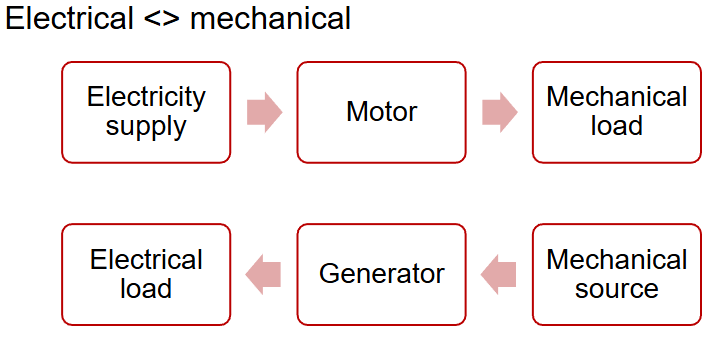
\includegraphics[width=0.5\textwidth]{assets/energieconversiemotorengenerator.png}
  \caption{Motor en generator energieconversie}
  \label{fig:energieconversiemotorengenerator.png}
 \end{figure}
Vaak zijn wel nog extra omvormers nodig voor de perfecte werking zoals \textit{Power eletronics} die bevoorbeeld eerst de spanning van een generator omvormt naar een andere spanning die nodig is voor de motor. En een tandwielkast kan ook nodig zijn om de snelheid van de motor aan te passen aan de toepassing. Hier gaan we niet dieper op in. Ook wordt vaak nog een controller gebruikt om de motor op een goeie manier te laten werken, dit is dus eigelijk \textit{terugkoppeling} (feedback).
\begin{figure}[H]
  \centering
  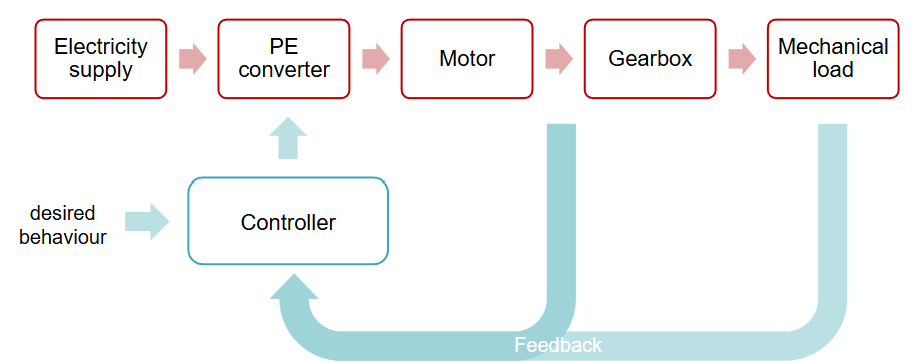
\includegraphics[width=0.6\textwidth]{assets/omzettingmetfeedback.png}
  \caption{Energieomzetting met feedback}
  \label{fig:omzettingmetfeedback.png}
 \end{figure}
Het vak gaat hier vooral over welk effect op de motor welk gedrag heeft op de uitgang (de 'mechanical load')
\section{Karakteristieken}
\subsection{Motor-last interactie}
Een motor moet dus een kracht leveren om deze beweging te realiseren. Met de wet van Newton kunnen we dit beschrijven en dus bepalen hoe hard de motor een object versnelt:
\begin{align*}
    \sum = F_{motor} - F_{load} = m \cdot a
\end{align*}
Hierbij is $F_{motor}$ de aandrijfkracht die de motor levert, $F_{load}$ de kracht die de last uitoefent op de motor (dus de 'tegenwerkende kracht van de belasting'), $m$ de massa van het object en $a$ de versnelling. Op een bepaald moment gaat de motor een constante snelheid bereiken (\textit{'Steady state'}), de versnelling wordt hier dan 0 en de krachten zijn in evenwicht. De motor levert dan een kracht die gelijk is aan de kracht van de last. De motor moet dus een koppel leveren dat gelijk is aan het koppel van de last. Het koppel van de motor wordt bepaald door de elektrische eigenschappen van de motor en de spanning die erop wordt gezet. Het koppel van de last wordt bepaald door de mechanische eigenschappen van de last en de snelheid waarmee deze beweegt. Volgend voorbeeld wordt aan bord in de les gemaakt:
\subsubsection{Voorbeeld Trein}
\textit{Een trein rijd met een constante snelheid van 40 km/h. De trein heeft een massa van 40 ton en de wrijving van de rails is 4 kN. Rijden vermeerderd die kracht met 20 kN in de positieve richting van de beweging, dit is dus de motorkracht. Wat is op dit moment de versnelling en wat gebeurt er daarna?}
\newline
We kunnen hier de wet van Newton toepassen:
\begin{align*}
    \sum = F_{motor} - F_{load} = m \cdot a
\end{align*}
We weten dat de massa van de trein 40 ton is, dit is 40000 kg. De kracht van de motor is 20 kN en de kracht van de last is 4 kN. We kunnen dit invullen in de vergelijking:
\begin{align*}
    20 kN - 4 kN = 40000 kg \cdot a
\end{align*}
\begin{align*}
    16 kN = 40000 kg \cdot a
\end{align*}
\begin{align*}
    a = \frac{16 kN}{40000 kg} = 0.4 m/s^2
\end{align*}
\subsubsection{Voorbeeld fiets}
Hier wordt een fiets gebruikt als voorbeeld, de proff geeft hier simpelweg het volgende:
\begin{align*}
    F_{motor} = 40 - 4 \cdot v
\end{align*}
Met motor de kracht op een pedaal door een persoon
\begin{align*}
  F_{load} = 10 + 0,4 \cdot v^2
\end{align*}
Met load de tegenwerkende kracht op een pedaal door bvb. de weg, fiets, mechanica van de fiets, etc.
\newline
Hier wordt gevraagd achter de regimesnelheid van de fiets (Steady State) (dus wanneer $a = 0$).
\begin{align*}
    F_{motor} = F_{load}
\end{align*}
\begin{align*}
    40 - 4 \cdot v = 10 + 0,4 \cdot v^2
\end{align*}
Dit geeft v = 5 m/s. Deze 2 krachten plotten in functie van de snelheid geeft een mooi overzicht van de krachten en hun snijpunt:
\begin{figure}[H]
  \centering
  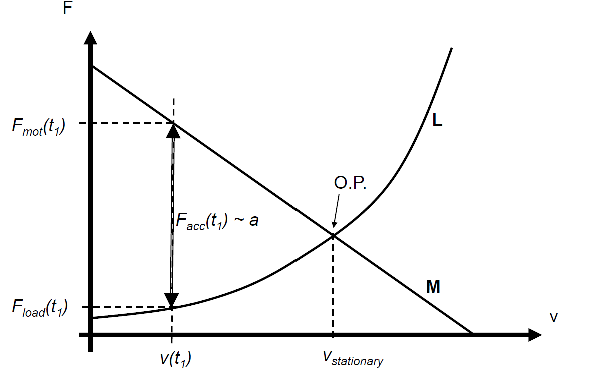
\includegraphics[width=0.6\textwidth]{assets/karakteristiekmetwerkingspunt.png}
  \caption{Krachten ifv snelheid}
  \label{fig:karakteristiekmetwerkingspunt.png}
 \end{figure}
O.P. is het \textbf{werkingspunt} (Operating Point), het is dus hier dat dat evenwicht is. Een \textbf{karakteristiek} is een grafiek/verzameling van grafieken die de relatie tussen 2 grootheden weergeeft alsook de werkingspunten. Een voorbeeld is de koppel-toerentalkarakteristiek van een motor.
\subsection{Werkingspunt}
Dus een werkingspunt is een evenwicht punt van de motor en de last. Voor een koppeltoerentalkarakteristiek zien we deze weergegeven als punt 1 en punt 2 in onderstaande figuur. Het zijn hier dus punten waar in dit geval de koppels van de last gelijk zijn aan die van de motor. Echter hebben we ook nog \textbf{stabiele} en \textbf{onstabiele} werkingspunten. Een stabiel werkingspunt is een werkingspunt waar bij afwijking van dat werkingspunt de motor en last elkaar nog gaan corrigeren en dus de motor terugbrengen naar dat werkingspunt. Neem als afwijking een snelheidsfout in punt 1, het toerental zal dalen tot punt 1', nu heeft de motor niet genoeg koppel meer om de last te dragen dus kan het niet terug versnellen tot punt 1, dit is dus een instabiel werkingspunt. Bij een snelheidsfout rond punt 2 is er oftewel genoeg koppel om te versnellen (punt 2') oftewel vertraagt de motor gewoon terug tot punt 2 als er een snelheidsfout tot punt 2'' was.
\begin{figure}[H]
  \centering
  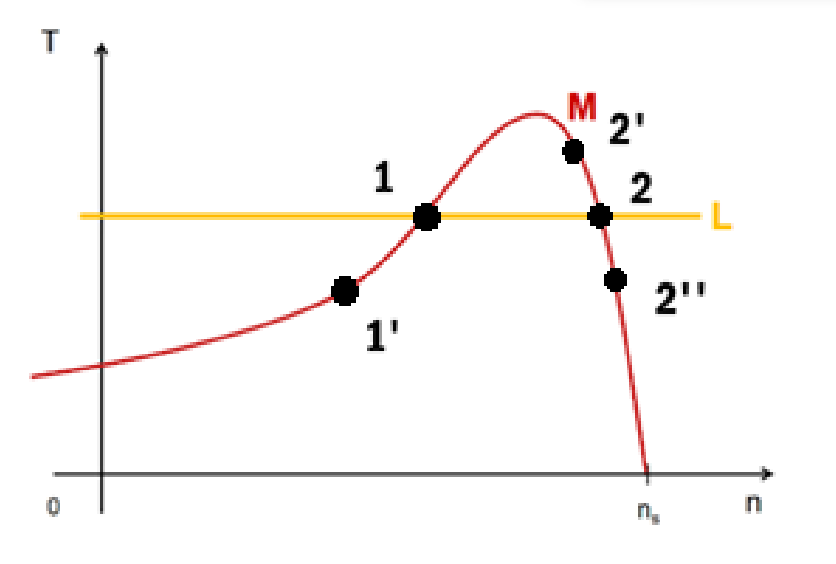
\includegraphics[width=0.6\textwidth]{assets/stabielenonstabielewerkingspuntenopTn.png}
  \caption{T-n karakteristiek motor en last met stabiele en onstabiele werkingspunten}
  \label{fig:stabielenonstabielewerkingspuntenopTn.png}
 \end{figure}
\subsection{Typische last karakteristieken}
In de les worden een paar typische lastkarakteristieken besproken:
\begin{figure}[H]
  \centering
  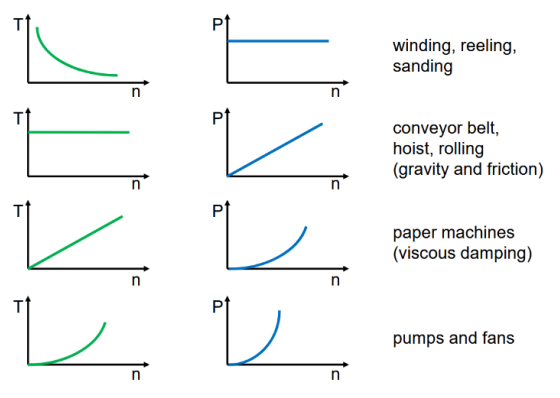
\includegraphics[width=0.4\textwidth]{assets/lastkarakteristieken.png}
  \caption{Typische lastkarakteristieken}
  \label{fig:lastkarakteristieken.png}
 \end{figure}
Veel diepgaand wordt het hier niet gesproken, gewoon dat die bovenste grafiek van 'winding, reeling, sanding' typisch een karakteristiek is van een geval waar de diameter steeds veranderd, hier is een constant vermogen, wat normaal niet vaak het geval is, de T-n ziet er dan hyperbolisch uit. En de 2de bovenste, die met het constante koppel, is de meest voorkomende karakteristiek, hierbij treedt voornamelijk zwaartekracht en wrijving op wat dus de meest voorkomende krachten zijn bij een machine.
\subsection{4 kwadrantoperaties}
Een elektrisch toestel (motor/generator) kan in 4 kwadranten werken, dit is afhankelijk van de richting van het koppel en de richting van de snelheid. In \textbf{kwadrant 1} werkt de motor als motor, dit is de \textit{normale werking}, het \textit{koppel is in dezelfde richting als de rotatie}, in \textbf{kwadrant 2} werkt de motor als generator, het \textit{koppel is in tegengestelde richting van de draairichting} (hier is het koppel positief) kwadrant 2 is dus remmend, in \textbf{kwadrant 3} werkt de motor als motor maar in tegengestelde richting en in \textbf{kwadrant 4} werkt de motor als generator maar in tegengestelde richting, het is hier dus een negatief koppel. Dit wordt vaak gebruikt bij elektrische voertuigen, waarbij de motor kan remmen \textbf{(regeneratief remmen)} en dus energie terug kan leveren aan de batterij.
\begin{figure}[H]
  \centering
  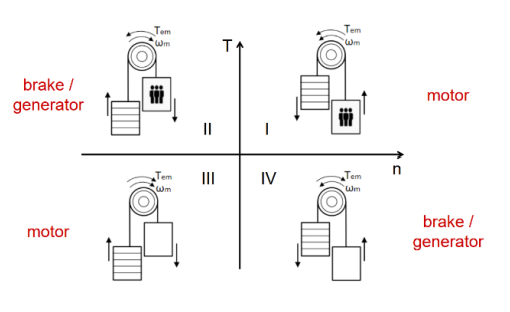
\includegraphics[width=0.5\textwidth]{assets/4kwadrantoperaties.png}
  \caption{4 kwadrantoperaties}
  \label{fig:4kwadrantoperaties.png}
 \end{figure}
\subsection{Nominale waardes}
De juiste motor voor je toepassing kiezen ga je doen afhankelijk van de eigenschappen van die motor: bvb. zoveel kW bij zoveel snelheid, motor selectie wordt dus met een catalogus gedaan, het toont dus eigelijk de waardes van de kenplaten van de motoren. Op zo een kenplaat staan \textbf{nominale waardes}, dit zijn de waardes waarvoor een motor ontwikkeld is om rond te werken. Dus eigelijk wat je continu kan doen. Indien je hoger dan deze nominale waardes gaat (dit kan) ga je rapper opwarmen, dit is niet gewenst want is slecht voor de motor dus je kan dit niet continu doen. Eigelijk zijn nominale waardes dus een \textit{thermische grens}. Belangrijk te weten is dus dat het vermogen van de motor niet constant is, het vermogen dat op de kentekenplaat staat is het nominale vermogen, en het vermogen bij gebruik kan anders zijn. Kleine machines wijken het meeste af (van nominale waardes voor snelheid bvb.), we zeggen dat ze een slechter \textbf{rendement} hebben.
\newline
\newline
Het rendement is eigelijk de \textbf{efficiëntie} van de motor, het is de verhouding van het nuttige vermogen dat uit de motor komt en het vermogen dat in de motor gaat. Het rendement is dus een maat voor hoe goed de motor energie omzet in nuttig werk. Het rendement wordt vaak uitgedrukt in procenten en kan berekend worden met de volgende formule:
\begin{align*}
    \eta = \frac{P_{out}}{P_{in}} \cdot 100\%
\end{align*}
Waarbij $\eta$ het rendement is, $P_{out}$ het nuttige vermogen dat uit de motor komt (eigelijk het mechanische vermogen) en $P_{in}$ het vermogen dat in de motor gaat (dus het elektrisch vermogen).
\begin{warningbox}[Het rendement en de arbeidsfactor zijn niet hetzelfde!]
    De arbeidsfactor bereken je met de formule:
    \begin{align*}
        \cos(\varphi) = \frac{P_{act}}{P_{schijn}}
    \end{align*}
    Numeriek lijken ze op elkaar maar ze zijn niet hetzelfde. Het rendement is een maat voor hoe goed de motor energie omzet in nuttig werk, terwijl de arbeidsfactor een maat is voor hoe goed de motor het elektrische vermogen gebruikt. Ze betekenen dus iets totaal anders.
\end{warningbox}
\section{Constructie}
\subsection{Motortypes}
Er zijn verschillende motortypes, vooral geclassificeerd op basis van hun voeding:
\begin{itemize}
 \item \textbf{AC Drie fasig}: Dit wordt vooral in de industrie gebruikt, deze hebben een beetje meer koper nodig dan een 1 fasige motor maar kunnen veel meer vermogen leveren.
 \item \textbf{AC Een fasig}: Dit wordt vooral in huishoudtoepassingen gebruikt.
 \item \textbf{DC}: Deze worden vooral gebruikt in voertuigen, zoals elektrische auto's, treinen, trams, etc. Ze hebben een goede regelbaarheid van het koppel en de snelheid.
 \item \textbf{Power Electronics}: (Op deze gingen we niet dieper in, het hoort wel bij deze motortypes)
\end{itemize}
Tussen de verschillende AC machines zijn er ook nog verschillende types, zoals \textbf{synchrone} (\textbf{Inductiemachine}) en \textbf{asynchrone} machines. Deze zien we later nog. Er zijn ook nog andere verschillende types die we niet echt bezien $\cdots$
\newline
\newline
Ook is er nog onderverdeling tussen Motoren en Generatoren.
\subsection{Constructie}
Een typische motor bestaat uit meerdere componenten die we aangeduid zien in de volgende figuur:
\begin{figure}[H]
  \centering
  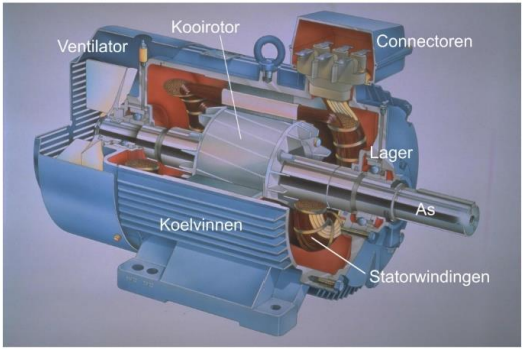
\includegraphics[width=0.6\textwidth]{assets/constructiemotor.png}
  \caption{Motor constructie inductiemachine}
  \label{fig:constructiemotor.png}
 \end{figure}
\begin{itemize}
 \item \textbf{Ventilator}: Dit dient om de motor te koelen, vooral belangrijk om de 'lak' / 'isolatie' van de wikkelingen niet te doen smelten.
 \item \textbf{Behuizing}: Dit dient om de motor te beschermen tegen stof, vuil, vocht, etc. Maar ook belangrijk om warmte af te voeren, daarom staan er ook vaak \textbf{koelvinnen} op de behuizing. Het moet dus belangrijke thermische eigenschappen hebben en bestaat dus uit \textbf{gietijzer}.
 \item \textbf{Rotor}: Dit is het draaiende deel van de motor, dat werkt op basis van elektromagnetisme. Het bestaat uit wikkelingen die door elektriciteit worden aangedreven. Hier zien we een \textbf{kooirotor} (het is dus een inductie motor), de stroom gaat dus door \textbf{Aluminium} (in een DC motor is dit koper).
 \item \textbf{Stator}: Dit is het stilstaande deel van de motor \textit{hier} (bij sommige motors is dit omgekeerd). Het zit binnenin de behuizing en bestaat uit \textbf{statorijzer} (\textit{Siliciumstaal}, dit is goed om magnetische veldlijnen te geleiden) (de kern) en \textbf{statorwikkelingen} (\textit{koper}) die in de gleuven van de kern liggen.
 \item \textbf{As/Shaft}: Dit is de as die de rotor aandrijft en het mechanische vermogen levert aan de belasting. Het is meestal gemaakt van \textbf{staal} en is verbonden met de rotor.
 \item \textbf{Lager}: Ondersteunt de as en zorgt dat deze soepel kan draaien.
 \item \textbf{Connectoren}: Deze dienen om de spanning aan te sluiten. In de meeste gevallen kunnen we hier ook kiezen of we de motor in ster of driehoek zetten.
\end{itemize}
\subsection{Magnetische Permeabiliteit}
Door het feit dat er een magnetisch veld wordt opgewekt in de motor, is het belangrijk dat de materialen die gebruikt worden een hoge magnetische permeabiliteit hebben. Dit betekent dat ze goed in staat zijn om magnetische veldlijnen te geleiden. Siliciumstaal wordt vaak gebruikt voor de kern van de stator en rotor omdat het een hoge permeabiliteit heeft en ook goed bestand is tegen verzadiging. Verzading treedt op wanneer het materiaal niet meer in staat is om extra magnetische flux te geleiden, wat kan leiden tot verlies van efficiëntie en warmteontwikkeling. Dat gietijzer zou enorme verliezen geven dus, daarom is het als behuizing prima want het is sterk en voert warmte goed af.
\newline
\newline
\newline
We zijn dus geïnteresseerd in ferromagnetische materialen, als we kijken naar de onderstaande figuur kunnen we zien hoe magnetische velden in een materiaal gealigneerd kunnen zijn:
\begin{figure}[H]
  \centering
  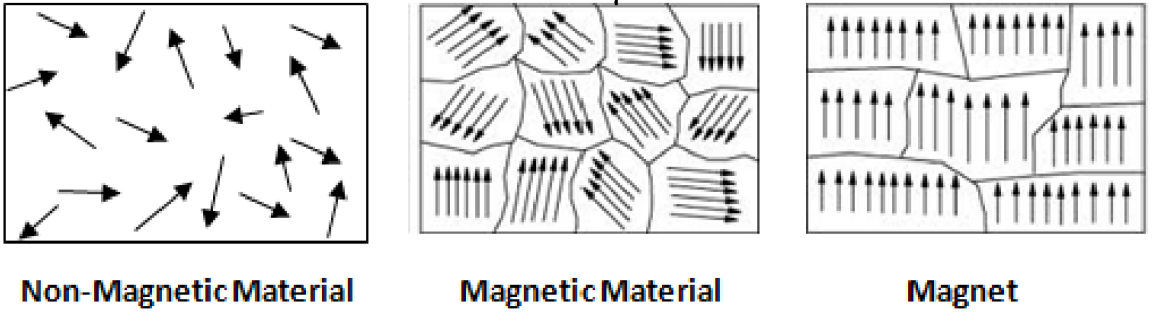
\includegraphics[width=0.8\textwidth]{assets/allignerenmagnetische-velden.png}
  \caption{Alligneren van de magnetische velden}
  \label{fig:allignerenmagnetische velden.png}
 \end{figure}
In de linkse figuur een niet ferro-magnetisch materiaal, alle pijlen zijn hier in alle richtingen gealigneerd (dit is op atomair niveau), geen netto magnetisch veld. In het midden een magnetisch materiaal hier zijn pijlen in groepjes verdeeld en elk groepje heeft een netto magnetisch veld maar het totaal geheel niet, dit kan wel gemagnetiseerd worden door een extern magnetisch veld. In de rechtse figuur is het materiaal volledig gealigneerd, dit is een permanent magneet. Het materiaal heeft hier een hoge permeabiliteit en kan dus goed magnetische flux geleiden. Doordat deze allemaal in dezelfde richting staan, is dit een sterk veld.
\newline
\newline
Het is dan dit fenomeen dat de permeabiliteit van een materiaal bepaalt, hoe beter de atomen in het materiaal zich kunnen aligeneren met het externe veld, hoe hoger de permeabiliteit. 
\begin{figure}[H]
  \centering
  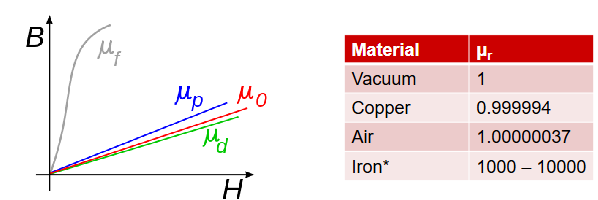
\includegraphics[width=0.8\textwidth]{assets/magnetischepermeabiliteit.png}
  \caption{Magnetische permeabiliteit van verschillende materialen (µ)}
  \label{fig:magnetischepermeabiliteit.png}
 \end{figure}
Hier is B de magnetische fluxdichtheid, H de magnetische veldsterkte en \textbf{µ de magnetische permeabiliteit}. De permeabiliteit van een materiaal is dus een maat voor hoe goed het materiaal in staat is om magnetische flux te geleiden. De helling zegt \textit{'hoeveel stroom je nodig hebt voor hoeveel magnetisch veld'}. En met dat magnetisch veld maak je dus de krachten die de motor doen draaien.
\newline
\newline
Nog iets belangrijks is de \textbf{hysteresis lus}, dit is een grafiek die de relatie tussen B en H weergeeft. Het toont ons echter ook de \textbf{remanente inductie}, dit is de magnetische flux die in het materiaal blijft nadat het externe veld is verwijderd. Dit is belangrijk omdat het kan leiden tot verlies van efficiëntie en warmteontwikkeling in de motor. Het toont ook de \textbf{coerciviteit}, dit is de kracht die nodig is om het materiaal te demagnetiseren (dus hoe hard we de veldsterkte moeten tegenwerken zodat de magnetische flux terug nul is). Materialen met een hoge coerciviteit zijn beter bestand tegen verzadiging en kunnen dus beter presteren in een motor.
\begin{figure}[H]
  \centering
  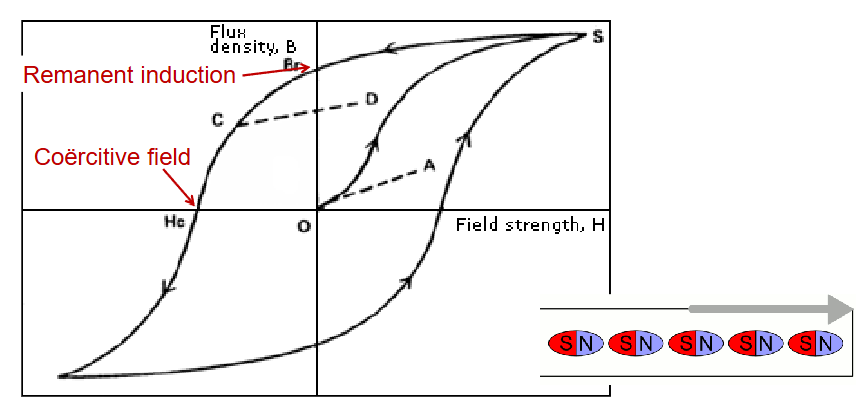
\includegraphics[width=0.5\textwidth]{assets/hysteresislus.png}
  \caption{Hysteresislus van een magnetisch materiaal}
  \label{fig:hysteresislus.png}
 \end{figure}
Een materiaal met een \textbf{kleine lus} noemen we een \textbf{zacht magnetisch materiaal}, dit is goed voor motoren. Een materiaal met een \textbf{grote lus} noemen we een \textbf{hard magnetisch materiaal}, dit is goed voor permanente magneten. De stator moet dus uit zo een zacht materiaal gemaakt worden aangezien dit op AC 50 keer de lus doet (50 Hz), dus dan hebben we minder verliezen. De rotor die volgt gewoon en dit kan met permanente magneten gedaan worden (kan ook met wikkelingen gedaan worden zoals de stator), dit is dan dus met een hard magnetisch materiaal (heeft een brede lus, magnetisch veld blijft, brede lus nodig dus).
\begin{figure}[H]
  \centering
  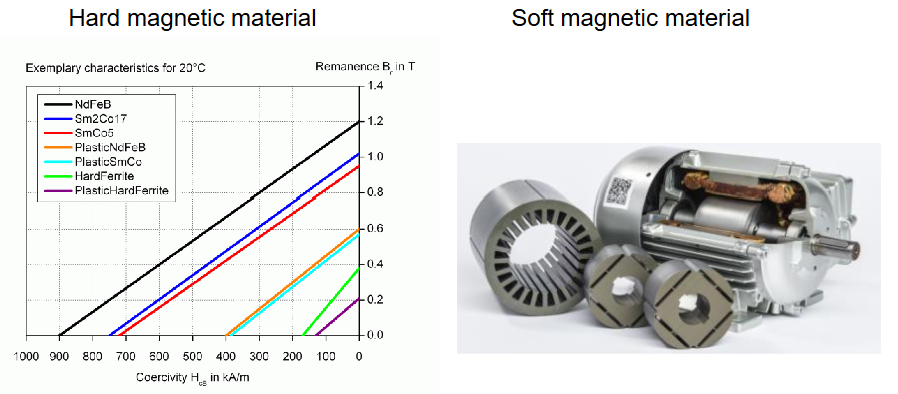
\includegraphics[width=0.8\textwidth]{assets/hardenzachtmagnmateriaak.png}
  \caption{Hard en zacht magnetisch materiaal}
  \label{fig:hardenzachtmagnmateriaak.png}
 \end{figure}
\subsection{Stator Constructie}
Dus de stator is het 'statische' deel van de motor, het bestaat dus uit die siliciumstaal kern met gleuven in, het heeft dus eigelijk 'statortanden', hierin bevestigen zich de statorwikkelingen. De statorwikkelingen zijn meestal van koper en zijn geïsoleerd om kortsluiting te voorkomen. De wikkelingen zijn zo geplaatst dat ze een magnetisch veld opwekken wanneer er stroom doorheen loopt. Dit magnetisch veld wisselt van richting afhankelijk van de stroomrichting, wat essentieel is voor de werking van de motor.
\begin{figure}[H]
  \centering
  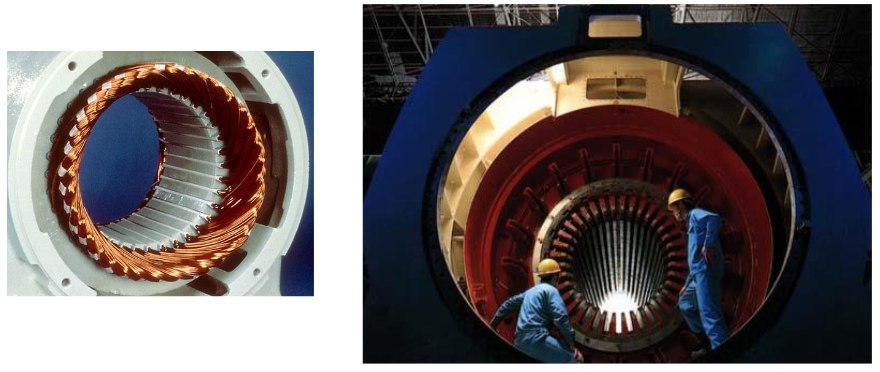
\includegraphics[width=0.6\textwidth]{assets/statorvisueel.png}
  \caption{Stator constructie met statortanden en wikkelingen}
  \label{fig:statorvisueel.png}
 \end{figure}
De wikkelingen kunnen op 2 manieren gewonden worden: 
\begin{itemize}
 \item \textbf{Geconcentreerd}: Hier heb je spoelen geconcentreerd rond individuele statortanden, het magnetisch veld opgewekt is dus eigelijk blokvormig, dus sterk recht per tand en niet zo mooi naast de tanden, het gevolg is een veld met veel harmonischen. Dit is goedkoper door minder koper maar heeft meer verliezen bij gebruik.
 \begin{figure}[H]
   \centering
   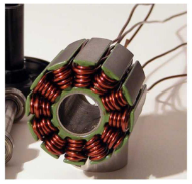
\includegraphics[width=0.4\textwidth]{assets/geconcentreerd.png}
   \caption{Geconcentreerde wikkelingen}
   \label{fig:geconcentreerd.png}
  \end{figure}
 \item \textbf{Gedistribueerd (verdeelde)}: Hier zijn de wikkelingen verdeeld over meerdere statortanden, er kunnen dus meerdere wikkelingen per gleuf op elkaar liggen, het magnetisch veld opgewekt is dus veel mooier en vloeiender, het gevolg is een veld met minder harmonischen. Dit is duurder door meer koper maar heeft minder verliezen bij gebruik.
 \begin{figure}[H]
   \centering
   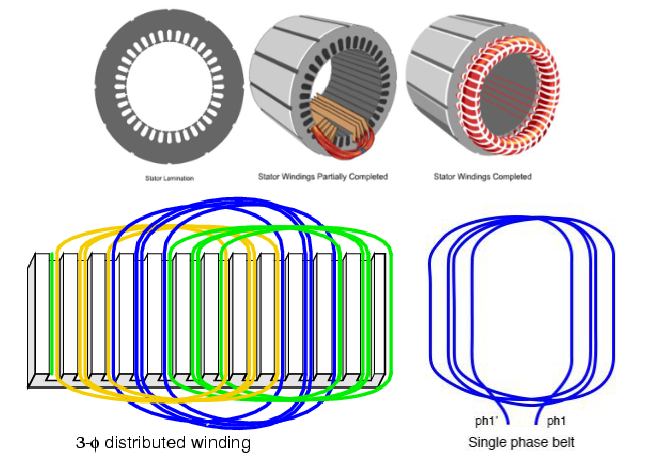
\includegraphics[width=0.6\textwidth]{assets/verdeelde.png}
   \caption{Gedistribueerde wikkelingen}
   \label{fig:verdeelde.png}
  \end{figure}
Meestal worden verdeelde wikkelingen gebruikt.
\end{itemize}
De statorkern zelf wordt in lamellen opgebouwd om wervelstromen te beperken (jouleverliezen), deze lamellen vormen samen nog steeds de blokvormige statorkern:
\begin{figure}[H]
  \centering
  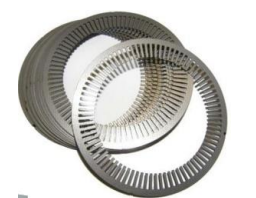
\includegraphics[width=0.4\textwidth]{assets/lamellenstator.png}
  \caption{Lamellen in de statorkern}
  \label{fig:lamellenstator.png}
 \end{figure}
\subsection{Rotor Constructie}
De stator constructie blijft vaak ongeveer hetzelfde maar bij de rotor is dit een ander verhaal, de constructie \textit{verschilt hier meer per machine/motortype.} Voor \textbf{de Synchrone machine} kan dit met \textbf{permanente magneten} of met \textbf{DC wikkelingen} gedaan worden.
\subsubsection{Permanente magneten}
Bij een rotor met permanente magneten zijn de magneten op de rotor bevestigd en zorgen ze voor een constant magnetisch veld. Dit type rotor is vaak compacter en efficiënter, maar kan duurder zijn vanwege de kosten van de permanente magneten. Hierbij kunnen we ook nog 2 types hebben:
\begin{itemize}
 \item \textbf{Uitspringende polen}: Hier heb je wat lucht tussen de polen, de magneten zijn er eigelijk opgeplakt, dit wordt het meest in de praktijk gebruikt want geeft een goede regeling (zien we later).
 \item \textbf{Gladde rotor}: Hier zijn geen gaten, de rotor is volledig dicht eigelijk, dit heeft als voordeel dat het 'magnetisch glad' is want dde veldlijnen komen direct ijzer tegen, dit maakt het symmetrischer.
\end{itemize}
\begin{figure}[H]
  \centering
  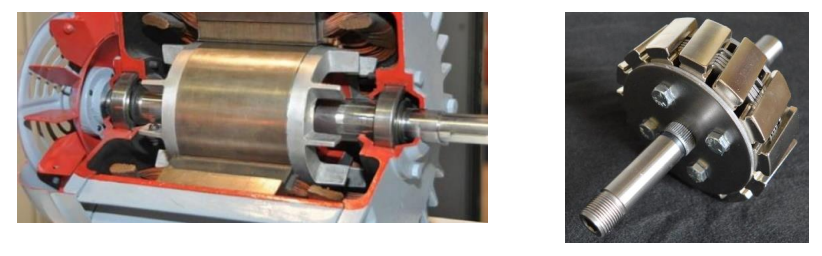
\includegraphics[width=0.8\textwidth]{assets/gladvsuitspringend.png}
  \caption{Gladde vs. uitspringende polen}
  \label{fig:gladvsuitspringend.png}
 \end{figure}
\subsubsection{DC Wikkelingen}
Dit is een rotor die wikkelingen er al op heeft staan en die gevoed worden met een DC-bron om een soort van permanente magneet te maken. Om deze constante stroom te voorzien worden \textbf{sleepringen} gebruikt, dit zijn metalen ringen (meestal koper) waar een \textbf{koolstofborstel} (dit roteert dus niet) op gedrukt wordt zodat de stroom van de DC-bron hierdoor naar de sleepringen van de rotor kan gaan.
\begin{figure}[H]
  \centering
  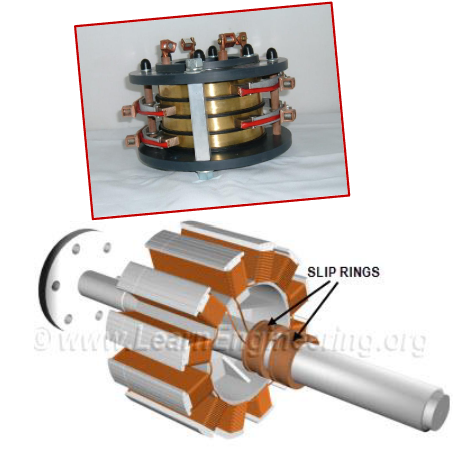
\includegraphics[width=0.4\textwidth]{assets/sleepringen.png}
  \caption{Sleepringen in de rotor}
  \label{fig:sleepringen.png}
 \end{figure}
Bij de \textbf{DC-machine} gebruiken we iets gelijkaardig, namelijk een \textbf{commutator} bij de constructie van de rotor:
\subsubsection{Commutator}
Het grote verschil met de sleepring hier is dat het onderbrekingen heeft, het wordt dus eigelijk gebruikt om wikkelingen op de rotor aan en uit te schakelen, dit is nodig om de stroomrichting in de rotorwikkelingen te veranderen zodat het magnetisch veld van de rotor altijd in dezelfde richting blijft ten opzichte van de stator. Dit is essentieel voor de werking van de DC-machine, omdat het ervoor zorgt dat het koppel constant blijft tijdens de rotatie. Ook hier worden koolstofborstels tegen geduwd. Een probleem is wel dat hier vonken kunnen onstaan.
\begin{figure}[H]
  \centering
  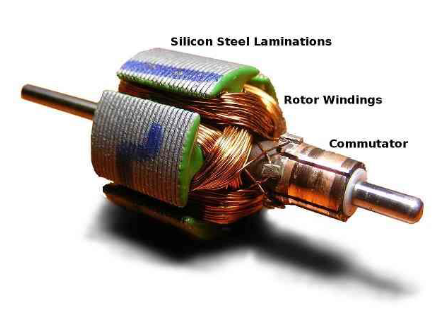
\includegraphics[width=0.4\textwidth]{assets/commutator.png}
  \caption{Commutator in de rotor}
  \label{fig:commutator.png}
 \end{figure}
\subsubsection{Inductiemachine}
Bij de \textbf{inductiemachine} kan de rotor een \textbf{kooirotor} of een \textbf{wikkelrotor} zijn. Bij de kooirotor zijn er geen wikkelingen op de rotor, maar geleiders die in een kooivormige structuur zijn geplaatst. Dit type rotor is robuuster en veel \textbf{goedkoper}, vooral door het productieproces want je giet dit gewoon in aluminium, het heeft ook geen sleepringen/commutator en geen onderhoud nodig, maar heeft minder regelbaarheid dan een wikkelrotor. Bij de wikkelrotor zijn er wikkelingen op de rotor die via sleepringen en koolstofborstels worden gevoed, dit geeft meer regelbaarheid maar is duurder en complexer.
\begin{figure}[H]
  \centering
  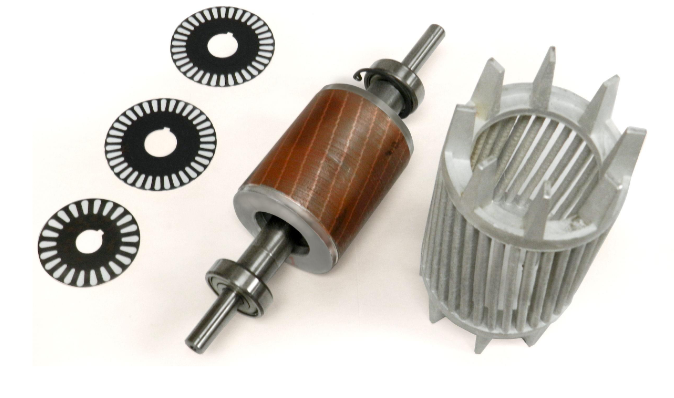
\includegraphics[width=0.5\textwidth]{assets/kooirotor.png}
  \caption{Kooirotor}
  \label{fig:kooirotor.png}
 \end{figure}
\begin{figure}[H]
  \centering
  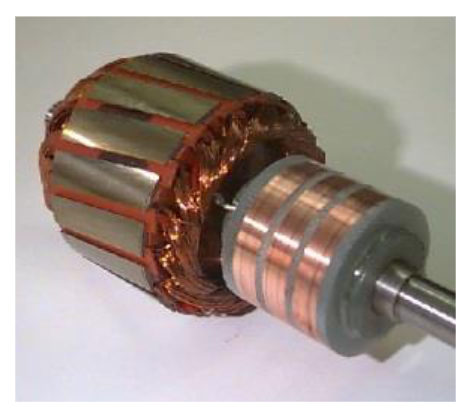
\includegraphics[width=0.4\textwidth]{assets/gewikkelderotor.png}
  \caption{Wikkelrotor}
  \label{fig:gewikkelderotor.png}
 \end{figure}
\newpage
\chapter{Gelijkstroommachines (DC Machines)}
DC-machines zijn dus elektrische machines die werken op een gelijkspanning, ze zijn makkelijk te regelen (vooral vroeger was dit zo, nu zijn andere motoren ook makkelijker regelbaar dus wordt deze machine minder gebruikt). Ze kunnen klein zijn en ook groot zijn, klein omdat ze permanente magneten gebruiken en zeldzame elementen (vaak niet zo duurzaam wel), het gewicht kan soms belangrijk zijn, wat die permanente magneten dus voordelig maakt.
\section{Werkingsprincipe}
Er zijn verschillende principes die zorgen voor de werking van de DC-machine, dit zijn de \textbf{wet van Faraday-Lenz}, \textbf{wet van Lorentz} en de \textbf{wet van Ampère}.
\subsection{Wet van Ampère}
Deze wet heeft niet direct veel invloed op de werking van de DC-machine (als je permanente magneten hebt!) maar is wel belangrijk om te weten. Deze wet beschrijft de relatie tussen een elektrische stroom en het magnetisch veld dat deze stroom opwekt. De wet van Ampère kan worden uitgedrukt met de volgende formule:
\begin{align*}
    \oint_l \vv{B} \cdot d\vv{l} = \mu_0 \cdot i
\end{align*}
Met de \textit{rechterhand regel} kan de richting van het magnetisch veld bepaald worden. Indien je geen permanente magneten gebruikt, gebruik je wikkelingen in de stator, het is juist deze wet dat dan eigelijk gebruikt wordt om het veld op te wekken en te bepalen hoe hard dat veld is. Moest je permanente magneten hebben is er inderdaad niet veel invloed op de werking maar gaat er wel nog steeds wat invloed zijn op het veld want de rotor heeft ook stroomvoerende geleiders, het totaal veld gaat een beetje vervormen (Ankerreactie) maar dit zien we later.
\begin{figure}[H]
  \centering
  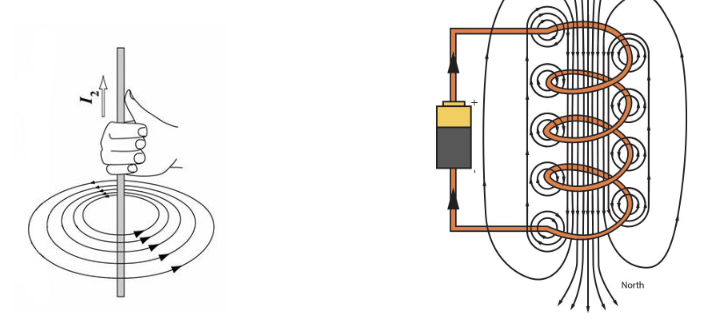
\includegraphics[width=0.6\textwidth]{assets/wetampere.png}
  \caption{Wet van Ampère}
  \label{fig:wetampere.png}
 \end{figure}
Dit kan ook zorgen voor wat lekflux, maar dit zien we later.
\subsection{Wet van Lorentz}
Vooraleer we naar het effectieve werkingsprincipe gaan kijken van de DC-motor, gaan we eerst kijken naar de wet van Lorentz. Deze wet beschrijft de kracht die een geladen deeltje ondervindt wanneer het zich in een magnetisch veld bevindt. De kracht wordt gegeven door de formule:
\begin{align*}
    \vv{F} = q \cdot \vv{E} + q \cdot \vv{v} \times \vv{B}
\end{align*}
Hierbij is $\vv{F}$ de kracht op het deeltje, $q$ de lading van het deeltje, $\vv{E}$ het elektrische veld, $\vv{v}$ de snelheid van het deeltje en $\vv{B}$ het magnetisch veld. Dit is niet echt belangrijk om te kennen maar wat wel belangrijk te weten is dat deze formule herschreven kan worden voor een stroomvoerende geleider in een magnetisch veld (een toepassing op de wet van Lorentz).:
\begin{align*}
    \vv{F} = I \cdot \vv{L} \times \vv{B}
\end{align*}
Hierbij is $I$ de stroom door de geleider, $\vv{L}$ de lengte van de geleider in het magnetisch veld en $\vv{B}$ het magnetisch veld. De kracht is dus loodrecht op zowel de stroomrichting als het magnetisch veld, dit is essentieel voor de werking van de motor, want hierdoor ontstaat er een koppel dat de rotor doet draaien. Met de \textit{Linkerhand regel} kan je de richting bepalen:
\begin{figure}[H]
  \centering
  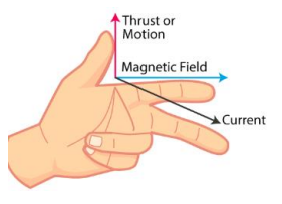
\includegraphics[width=0.3\textwidth]{assets/linkerhandregel.png}
  \caption{Linkerhandregel}
  \label{fig:linkerhandregel.png}
 \end{figure}
Als we nu zo een stroomvoerende geleider in een lus in een magnetisch veld plaatsen, zal er een moment ontstaan dat de lus doet draaien. Dit is het basisprincipe van de DC-motor. De richting van de stroom en het magnetisch veld bepalen de draairichting van de motor. De volledige bewerking van het uiteindelijk resultaat van dat moment ga ik hier niet uitrekenen maar op de slide staat dan dat het moment uitendelijk als volgt beschreven wordt:
\begin{align*}
    M = N \cdot i \cdot S \cdot B \cdot sin(\theta)
\end{align*}
Hierbij is $M$ het koppel, $N$ het aantal windingen in de lus, $S$ het oppervlak van de lus, $i$ de stroom door de lus, $B$ de magnetische fluxdichtheid en $\theta$ de hoek tussen het oppervlak van de lus en het magnetisch veld.
\begin{figure}[H]
  \centering
  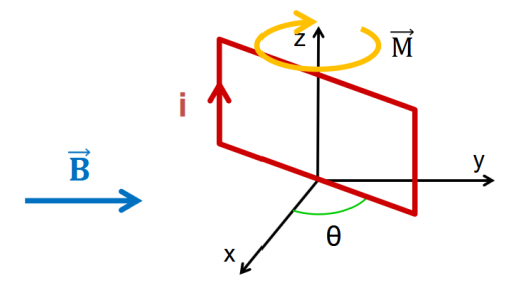
\includegraphics[width=0.4\textwidth]{assets/strromlus.png}
  \caption{Stroomlus in een magnetisch veld}
  \label{fig:strromlus.png}
 \end{figure}
\newpage
\subsection{Wet van Faraday-Lenz}
De laatste wet die we nodig hebben is die van Faraday-Lenz. Deze beschrijft dat er een spanning (EMK) wordt opgewekt wanneer een geleider door een magnetisch veld beweegt, en dat die opgewekte spanning zich volgens Lenz net zo richt dat ze de oorzaak tegenwerkt. Voor een geleider die met een snelheid $v$ door een veld $B$ beweegt, geldt:
\begin{align*}
    e = B \cdot l \cdot v
\end{align*}
Hierbij is $e$ de opgewekte spanning (EMK), $B$ de magnetische fluxdichtheid, $l$ de lengte van de geleider in het veld en $v$ de snelheid waarmee de geleider beweegt. (Dit komt eigelijk van $\vv{E} = \vv{v} \times \vv{B}$, en de vorm $e = B \cdot l \cdot v$ klopt alleen als alles loodrecht is.)

In de DC-motor speelt dit een belangrijke rol. Zodra de rotor draait, bewegen zijn geleiders door het magnetisch veld, en volgens de formule hierboven wekken ze dus zelf een spanning op. Volgens Lenz is die tegengesteld aan de aangelegde voedingsspanning, en daarom noemen we ze de \textbf{tegen-EMK} (of back-EMF). Hoe sneller de rotor draait (grotere $v$), hoe groter deze tegen-EMK.

De aangelegde spanning $U$ moet dus in evenwicht zijn met deze tegen-EMK $E$ plus de spanningsval over de ankerweerstand $R$:
\begin{align*}
    U = E + I \cdot R
\end{align*}
Hieruit volgt meteen het gedrag van de motor. Bij het opstarten staat de rotor stil, dus $v = 0$ en $E = 0$, waardoor de aanloopstroom $I = U/R$ heel groot is. Naarmate de motor op snelheid komt, stijgt $E$, wordt $(U - E)$ kleiner en daalt de stroom vanzelf. De motor regelt zichzelf dus: hij trekt net genoeg stroom voor de belasting die op de as staat.

Ten slotte toont deze wet ook de \textbf{dualiteit motor--generator}. Dezelfde machine kan in twee richtingen werken. Als motor stop je er elektrische energie in en komt er mechanische energie (koppel) uit, waarbij de tegen-EMK een neveneffect is dat de stroom begrenst. Draai je de as daarentegen mechanisch aan, dan beweegt de geleider door het veld en wekt de machine via $e = B l v$ zelf een spanning op die je kunt afnemen: ze werkt dan als \textbf{generator}. De tegen-EMK in een draaiende motor is eigenlijk het bewijs dat die generatorwerking er altijd al in zit; enkel de energierichting keert om.
\begin{figure}[H]
  \centering
  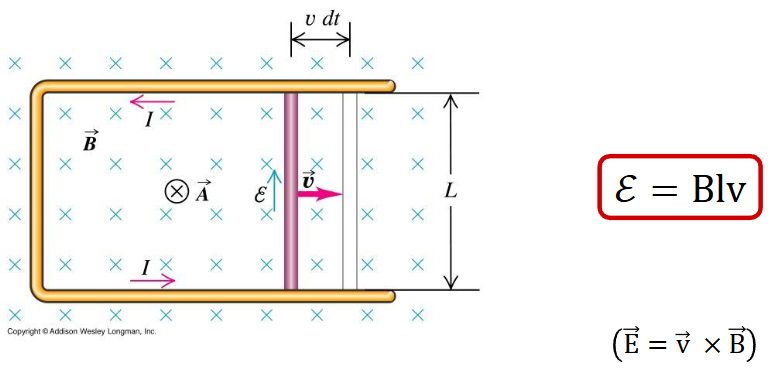
\includegraphics[width=0.6\textwidth]{assets/wetfaradaylenz.png}
  \caption{Werkingsprincipe Faraday-Lenz}
  \label{fig:wetfaradaylenz.png}
 \end{figure}
\subsection{Werkingsprincipe DC-motor}
Met deze wetten kan dus nu de werkingsprincipe van de DC-motor volledig verklaard worden, ook duidelijk in de volgende figuur:
\begin{figure}[H]
  \centering
  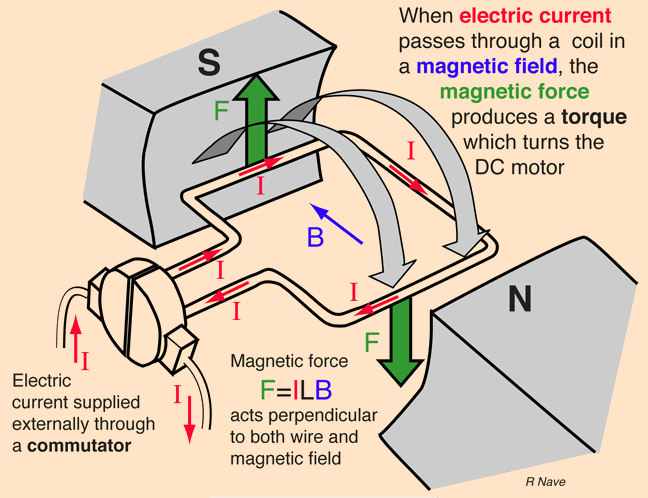
\includegraphics[width=0.5\textwidth]{assets/Faradaylenz.png}
  \caption{Werkingsprincipe DC-motor}
  \label{fig:Faradaylenz.png}
 \end{figure}
We zien hier dus een stroomvoerende lus in een magnetisch veld, de wet van Lorentz zegt dat er dan een resulterende kracht is, die dus een moment genereert dat de motor doet draaien. De stroom wordt daar aangelegd met een \textbf{commutator} deze zorgt ervoor dat de stroomrichting in de lus altijd zo is dat het moment in dezelfde richting blijft, dus de stroomrichting in de lus wordt steeds omgekeerd als de lus een halve rotatie heeft gemaakt. Ook is er lekflux door de wet van Ampère en hebben we dus ook een tegen-emk.
\begin{figure}[H]
  \centering
  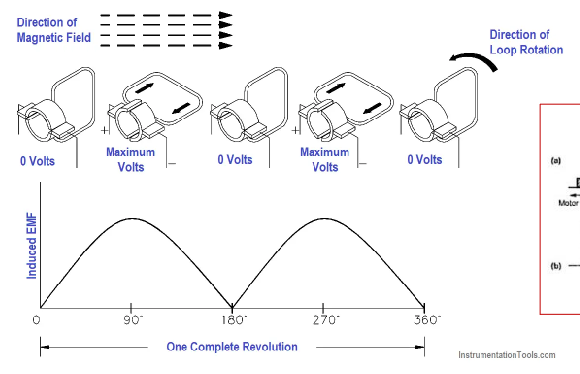
\includegraphics[width=0.6\textwidth]{assets/commutatorenemk.png}
  \caption{Commutator en geïnduceerd tegen-EMK in de DC-motor}
  \label{fig:commutatorenemk.png}
 \end{figure}
In de figuur hierboven zien we fysisch hoe die commutator werkt en ook het verloop van de tegen-emk, je ziet dat de tegen-emk minimaal is daar waar de stroom door de lus net nul is. Dit is dus eigelijk ook voor 1 lus gerepresenteerd. \textit{Een commutator is eigelijk een mechanische gelijkrichter.}
\newline
\newline
Voor meerdere wikkelingen, waar we dus sneller wisselen met commutatoren gaan we een tegen-emk krijgen zoals op de volgende figuur:
\begin{figure}[H]
  \centering
  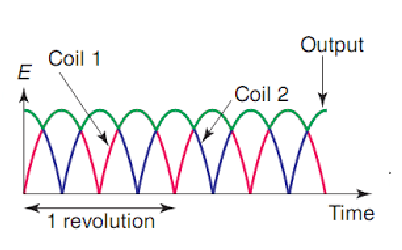
\includegraphics[width=0.6\textwidth]{assets/tegenemkmeerdere.png}
  \caption{Tegen-EMK in DC-motor met meerdere wikkelingen}
  \label{fig:tegenemkmeerdere.png}
 \end{figure}
Dit is dus een meer vlakkere curve, dit geldt dus ook voor het koppel:
\begin{figure}[H]
  \centering
  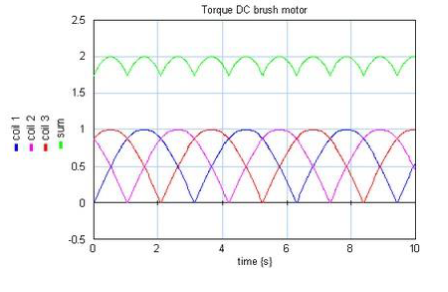
\includegraphics[width=0.6\textwidth]{assets/koppelmeerderelusse.png}
  \caption{Koppel in DC-motor met meerdere wikkelingen}
  \label{fig:koppelmeerderelusse.png}
 \end{figure}
Hier een close-up van de commutator, je ziet hier de koolstofborstels die er tegen duwen zodat de stroom van de voeding naar de rotor kan gaan, je ziet ook een veer dat zorgt dat de koolstofborstel goed tegen de commutator blijft duwen.
\begin{figure}[H]
  \centering
  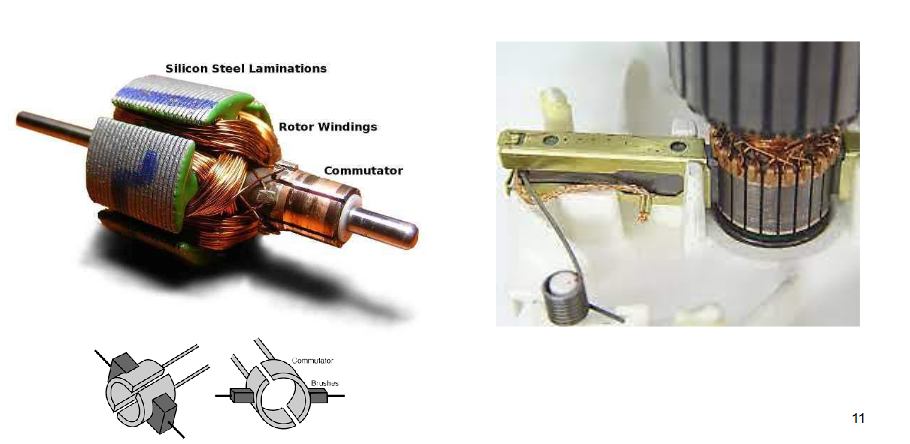
\includegraphics[width=0.6\textwidth]{assets/closeupcommutator.png}
  \caption{Close-up commutator}
  \label{fig:closeupcommutator.png}
 \end{figure}
\section{Constructie}
Dan gaan we nu eens de constructie van de DC-machine overlopen, we weten dus dat er een stator en een rotor is, deze kunnen we ook zien in de volgende figuur:
\begin{figure}[H]
  \centering
  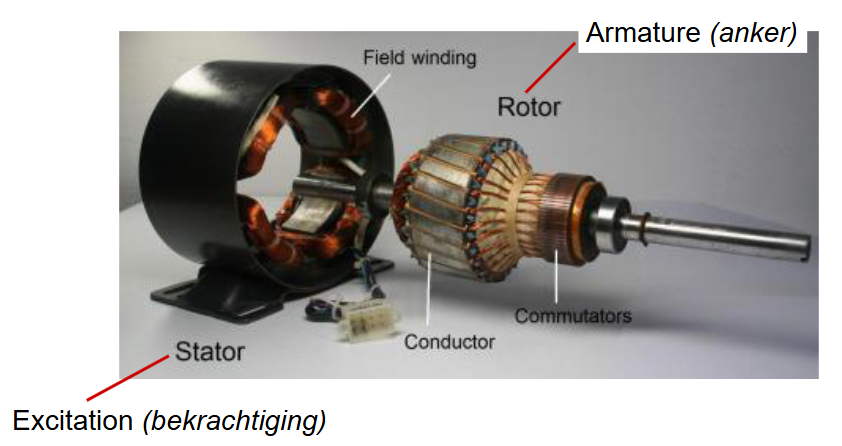
\includegraphics[width=0.6\textwidth]{assets/statorenrotordcmachine.png}
  \caption{Constructie van de DC-machine}
  \label{fig:statorenrotordcmachine.png}
 \end{figure}
De \textit{stator} staat bij de DC-machine \textit{vast} en bestaat meestal uit geconcentreerde wikkelingen, bij de DC-machine wordt deze altijd de \textbf{excitatie}, \textbf{bekrachtiging} of het \textbf{veld} genoemd. Die benaming komt van het feit dat je de wikkelingen in de stator een magnetisch veld doet opwekken (als het dus met wikkelingen is).
\begin{figure}[H]
  \centering
  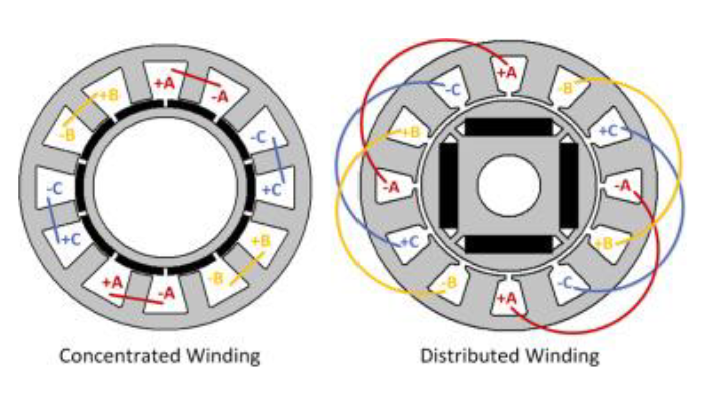
\includegraphics[width=0.6\textwidth]{assets/concrentregedstribitureed.png}
  \caption{Extra weergave van de statorconstructie met geconcentreerde en verdeelde wikkelingen}
  \label{fig:concrentregedstribitureed.png}
 \end{figure}
De \textit{rotor} is hier het draaiende deel van de machine, bij de DC-machine wordt deze altijd het \textbf{anker} genoemd. De rotor is bevestigd in de stator en draait rond een as. We zien op de figuur hier ook nog de commutators (er zijn meerdere wikkelingen).
\newline
\newline
Nog een eigenschap van een DC-machine is het \textbf{poolpaartal} (hoeveel duos van polen), die polen vormen het magnetisch veld (elk pool maakt een veld), maar je kan dus meerdere poolpaartallen hebben, meer poolpaartallen zorgen er ook voor dat je de motor trager kan laten draaien. Elk poolpaar geeft namelijk één veldwisseling per omwenteling, dus met meer polen ziet de rotor meer veldwisselingen per toer. Zo maakt de machine nog genoeg spanning en koppel, zelfs als de as traag draait. Met weinig polen zou je bij die lage snelheid te weinig veldwisselingen hebben en zou je de motor juist snel moeten laten draaien. Daarom vind je veel polen vooral bij grote, traag draaiende machines met veel koppel.
\newpage
Er zijn wel nadelen aan veel polen. Elke pool neemt met zijn wikkeling plaats in op de omtrek, dus heb je een grotere diameter nodig om ze kwijt te kunnen. Ook keert het veld sneller om in de rotor, wat meer ijzerverliezen geeft. Voor een gewone, snelle en compacte motor houd je het poolpaartal dus liefst laag, typisch 2 tot 8 polen max.
\begin{figure}[H]
  \centering
  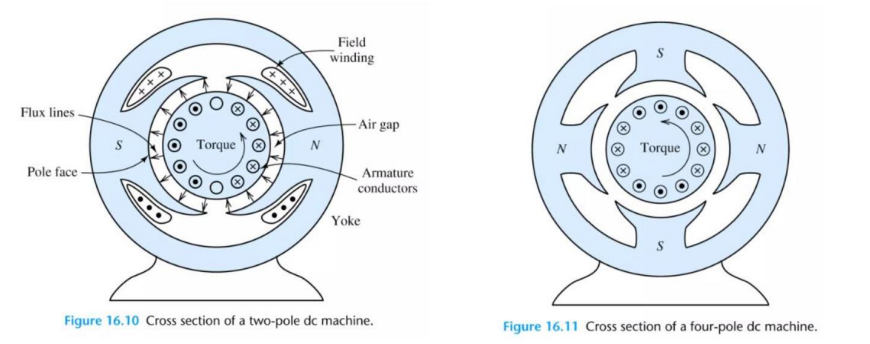
\includegraphics[width=0.6\textwidth]{assets/1en2poolpaartallendcmotor.png}
  \caption{DC-motor met 1 en 2 poolparen}
  \label{fig:1en2poolpaartallendcmotor.png}
 \end{figure}
Nog iets dat belangrijk is zijn de wikkelingen van de rotor, deze kunnen op verschillende manieren verbonden zijn. Het bepalen van hoe je ze verbindt hangt af van de gewenste nominale waarden voor spanning, stroom, vermogen, enz. Het wikkelen van de rotor kan er namelijk voor zorgen dat er minder stroom door elke individuele geleider gaat. Dit wordt duidelijker in de volgende figuur:
\begin{figure}[H]
  \centering
  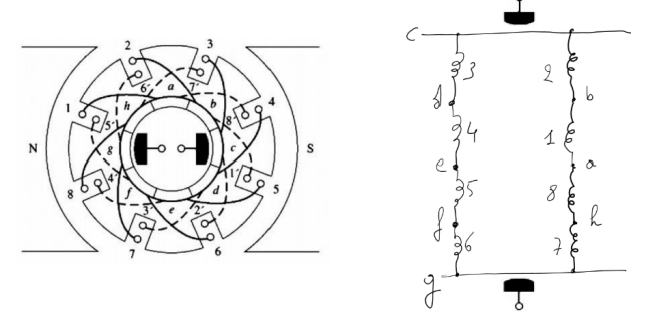
\includegraphics[width=0.8\textwidth]{assets/rotorwikkeling2poligiemotor.png}
  \caption{Rotorwikkeling van een 2-polige DC-motor}
  \label{fig:rotorwikkeling2poligiemotor.png}
 \end{figure}
Hierboven zien we een specifieke rotorwikkeling van een 2-polige DC-motor. De 2 zwarte blokjes zijn eigenlijk de koolstofborstels op de commutator: als het rechterblokje de + is, dan is het linkerblokje de -. De verbinding gebeurt dan als volgt: $+ \rightarrow 3 \rightarrow 3' \rightarrow 4 \rightarrow 4' \rightarrow 5 \rightarrow \cdots$. We krijgen zo de schematische opstelling die we rechts zien: 2 parallelle takken, waardoor de stroom zich kan verdelen. 
\section{Motor model en karakteristieken}
Om berekeningen in de praktijk vlotter te doen gaan we nu eens van ons meer fysisch model dat we eerder hadden uitgelegd naar een mathematisch model gaan en effectief de formules bezien. Hiermee kunnen we dan uiteindelijk een equivalent schema opstellen en de karakteristieken van de motor bepalen.
\subsection{Koppel}
We weten dat het koppel van de motor beschreven kan worden als:
\begin{align*}
    T = N \cdot F \cdot 2 \cdot r
\end{align*}
Hierbij is $T$ het koppel, $N$ het aantal windingen, $F$ de kracht op de geleider en $r$ de straal van de rotor. Nu weten we dat de kracht op de geleider kan worden beschreven met de wet van Lorentz:
\begin{align*}
    T = N \cdot i_a \cdot l \cdot B \cdot 2 \cdot r
\end{align*}
Hierbij is $i_a$ de stroom door de ankerwikkeling, $l$ de 'actieve' lengte van de rotorgeleider en $B$ de magnetische fluxdichtheid. Met 'actieve' bedoelen we dus het deel van de geleider waar dus effectief een tegen-emk wordt geïnduceerd. Om dit te verduidelijken tekent de proff het volgende aan bord:
\begin{figure}[H]
  \centering
  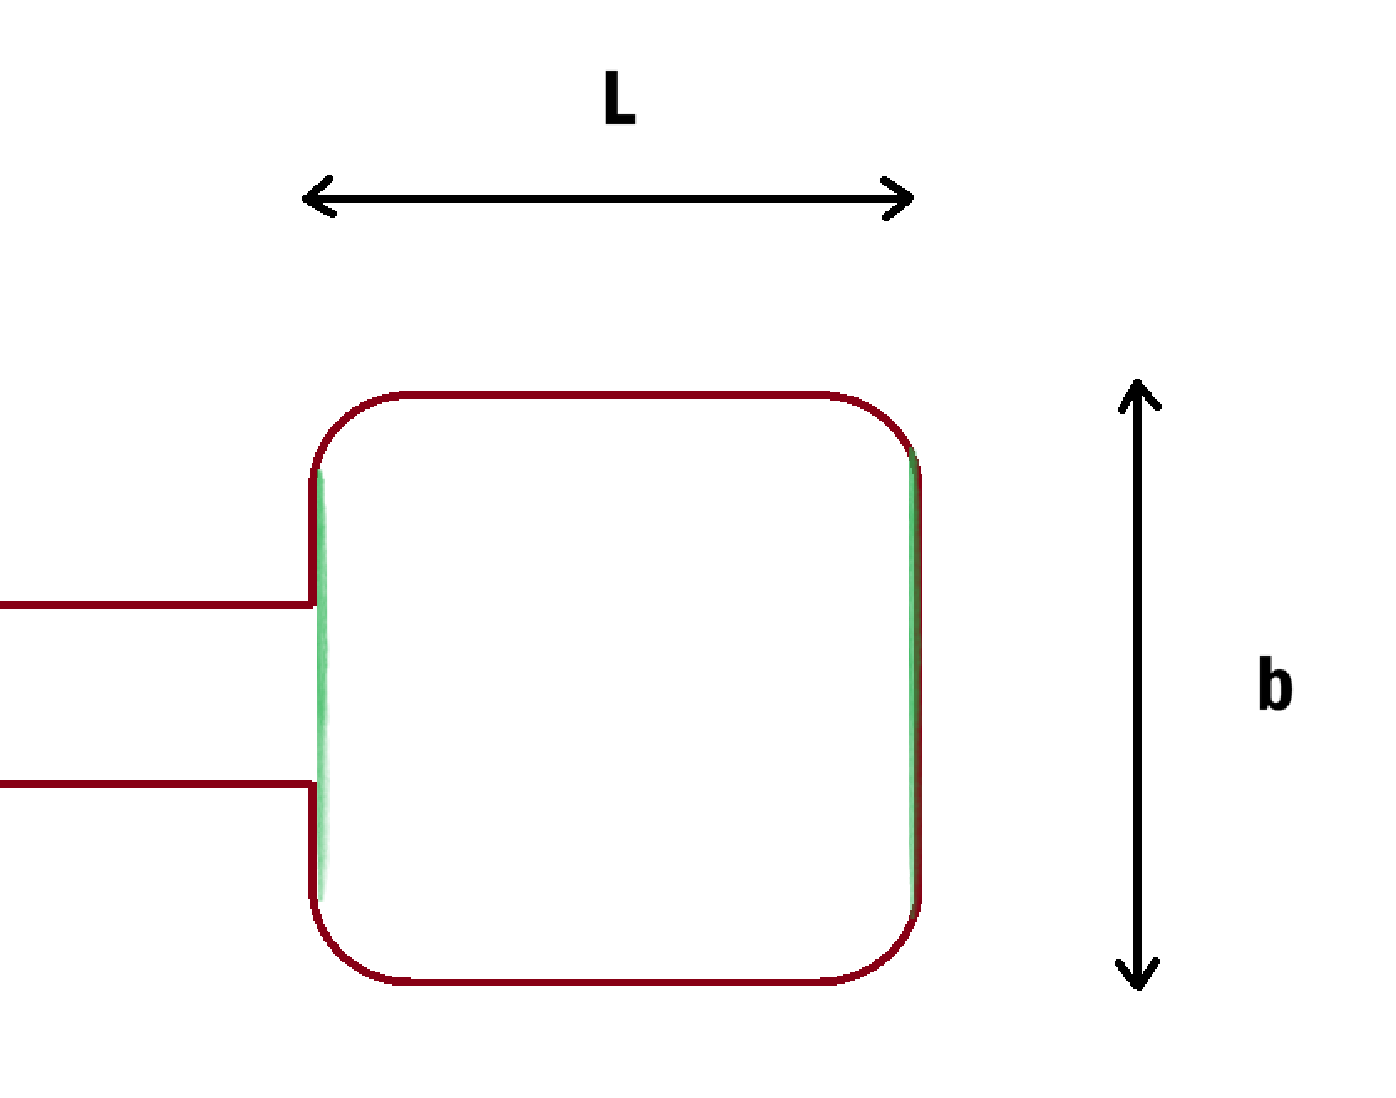
\includegraphics[width=0.4\textwidth]{assets/luswikkeling.png}
  \caption{1 wikkeling van de rotor}
  \label{fig:luswikkeling.png}
 \end{figure}
Het groen gearceerde heeft hier netto geen tegen-emk dat geïnduceerd wordt, het is dus niet actief. Het deel dat wel actief is, is het deel dat loodrecht staat op de veldlijnen van het magnetisch veld. Ook die $2r$ en l zijn samen eigelijk een oppervlakte en een oppervlakte vermenigvuldigd met de magnetische inductie B is dus een flux, we kunnen dit dus herschrijven als:
\begin{align*}
    T = K \cdot \varphi \cdot i_a
\end{align*}
Hierbij is K een constante (soms wordt er ook C gebruikt)
\newline
\newline
Ook weten we dat deze flux $\varphi$ evenredig is met de veldstroom $i_f$ (of $i_e$) (de stroom door de statorwikkelingen), dus we kunnen dit herschrijven als:
\begin{align*}
    T = G \cdot i_e \cdot i_a
\end{align*}
\newpage
\subsection{Tegen-EMK}
Met de wet van Faraday-Lenz kunnen we de tegen-EMK van de motor beschrijven als:
\begin{align*}
    E = B \cdot l \cdot v
\end{align*}
Alles moet wel loodrecht staan! Bij een rotatie geldt ook dat de snelheid $v$ van de geleider kan worden beschreven als:
\begin{align*}
    v = \omega \cdot r
\end{align*}
Hierbij is $\omega$ de hoeksnelheid van de rotor en $r$ de straal van de rotor. Ook weten we dat $l \cdot 2 \cdot r$ de oppervlakte van de lus is, en dat $B \cdot A$ de flux door de lus is, dus we kunnen dit herschrijven als:
\begin{align*}
    E = K \cdot \varphi \cdot \omega
\end{align*}
Deze K is dezelfde constante als bij het koppel, dit is dus een constante die afhankelijk is van de constructie van de motor. Dit is 'interessant' bij DC-machines zegt de proff.
\subsection{Klemspanning}
Met de wetten van Kirchoff (KVL) kunnen we de klemspanning van de motor beschrijven als:
\begin{align*}
   U_a = E + R_a \cdot i_a + {\color{red}L_a \cdot \frac{di_a}{dt}}
\end{align*}
Hierbij is $U_a$ de klemspanning (van het anker dus), $E$ de tegen-emk die we eerder beschreven hebben, $R_a$ de weerstand van de ankerwikkeling, $L_a$ de inductantie van de ankerwikkeling en $i_a$ de stroom door de ankerwikkeling. De term $L_a \cdot \frac{di_a}{dt}$ vertegenwoordigt de spanningsval over de inductantie van de ankerwikkeling die geïnduceerd wordt, die optreedt wanneer de stroom door de wikkeling verandert. Deze is verwaarloosbaar bij een DC-machine omdat die zo klein is en dus niet bijdraagt aan de klemspanning. De effectieve formule die we gaan gebruiken voor de klemspanning is dus:
\begin{align*}
   U_a = E + R_a \cdot i_a
\end{align*}
Met deze 3 vergelijkingen kunnen we de hele DC-machine beschrijven, ook is het ideaal dat deze allemaal lineair zijn.
\newpage
\subsection{Equivalent Schema}
Het opgestelde equivalent schema ziet er als volgt uit:
\begin{figure}[H]
  \centering
  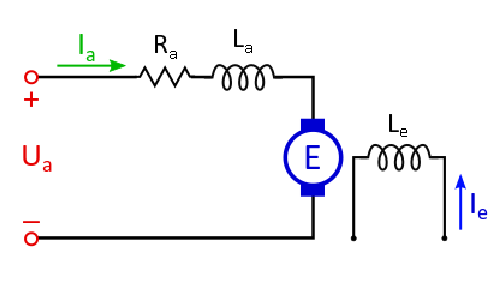
\includegraphics[width=0.6\textwidth]{assets/equivalentschemaDC.png}
  \caption{Equivalent schema van de DC-machine}
  \label{fig:equivalentschemaDC.png}
 \end{figure}
Het linkse gedeelte representeert het \textit{Rotormodel} en het rechtse gedeelte representeert het \textit{Statormodel}. Bij het statormodel is er eigelijk ook nog een weerstand in serie met $L_e$ ($R_e$) en wat ook niet super duidelijk is, maar wel belangrijk te weten is dat die stator ook nog gevoed wordt (veldvoeding), maar de manier waarop deze gevoed wordt kan verschillen (dit zien we zometeen). Bij dat rotormodel zijn die 2 blauwe blokjes bij E de weergave van de koolstofborstels. De tegen-emk wordt eigelijk als spanningsbron gemodelleerd.
\subsection{DC-motor types}
Er zijn ook verschillende soorten motoren en \textit{bekrachtigingen} (hoe de stator wordt gevoed, dus de excitatie). De bekrachtiging kan op verschillende manieren gebeuren, dit zijn de volgende:
\begin{itemize}
  \item \textbf{Aparte excitatie}: Oftewel 'onafhankelijke bekrachtiging', hierbij wordt het anker en de excitatie door een andere bron gevoed, onafhankelijk van elkaar dus. Zelfde schema als eerder dus ook, alleen daar bij het statormodel gewoon een aparte voeding verbinden.
  \item \textbf{Shunt excitatie}: Hierbij plaatsen we de excitatie en het anker in parallel, dit heeft als voordeel een constante flux, dus het koppel is lineair met de ankerstroom, en de snelheid blijft vrij stabiel ongeacht van de belasting. Ideaal voor als je een constante snelheid wilt.
  \begin{figure}[H]
    \centering
    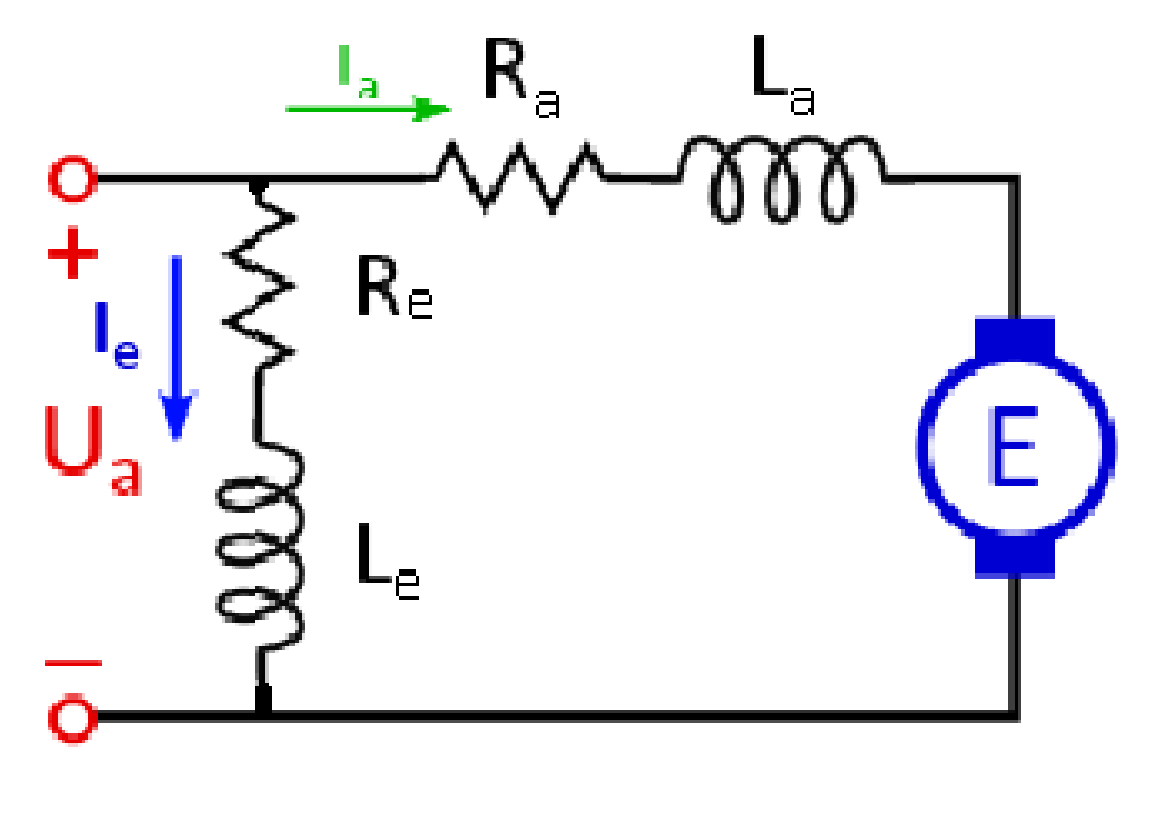
\includegraphics[width=0.5\textwidth]{assets/shuntbekrachtiging.png}
    \caption{Shunt bekrachtiging van een DC-machine}
    \label{fig:shuntbekrachtiging.png}
   \end{figure} 
   \newpage
   \item \textbf{Serie excitatie}: Hierbij plaatsen we de excitatie en het anker in serie, dit heeft als voordeel dat de excitatiestroom gelijk is aan de ankerstroom, waardoor met $T = G \cdot i_e \cdot i_a$ het koppel kwadratisch stijgt met de stroom, waardoor er een groot startkoppel ontstaat bij lage snelheid/stilstand en dit koppel dan sterk daalt als de snelheid stijgt, perfect voor toepassingen die veel kracht nodig hebben om te starten maar daarna minder zoals een trein.
  \begin{figure}[H]
     \centering
     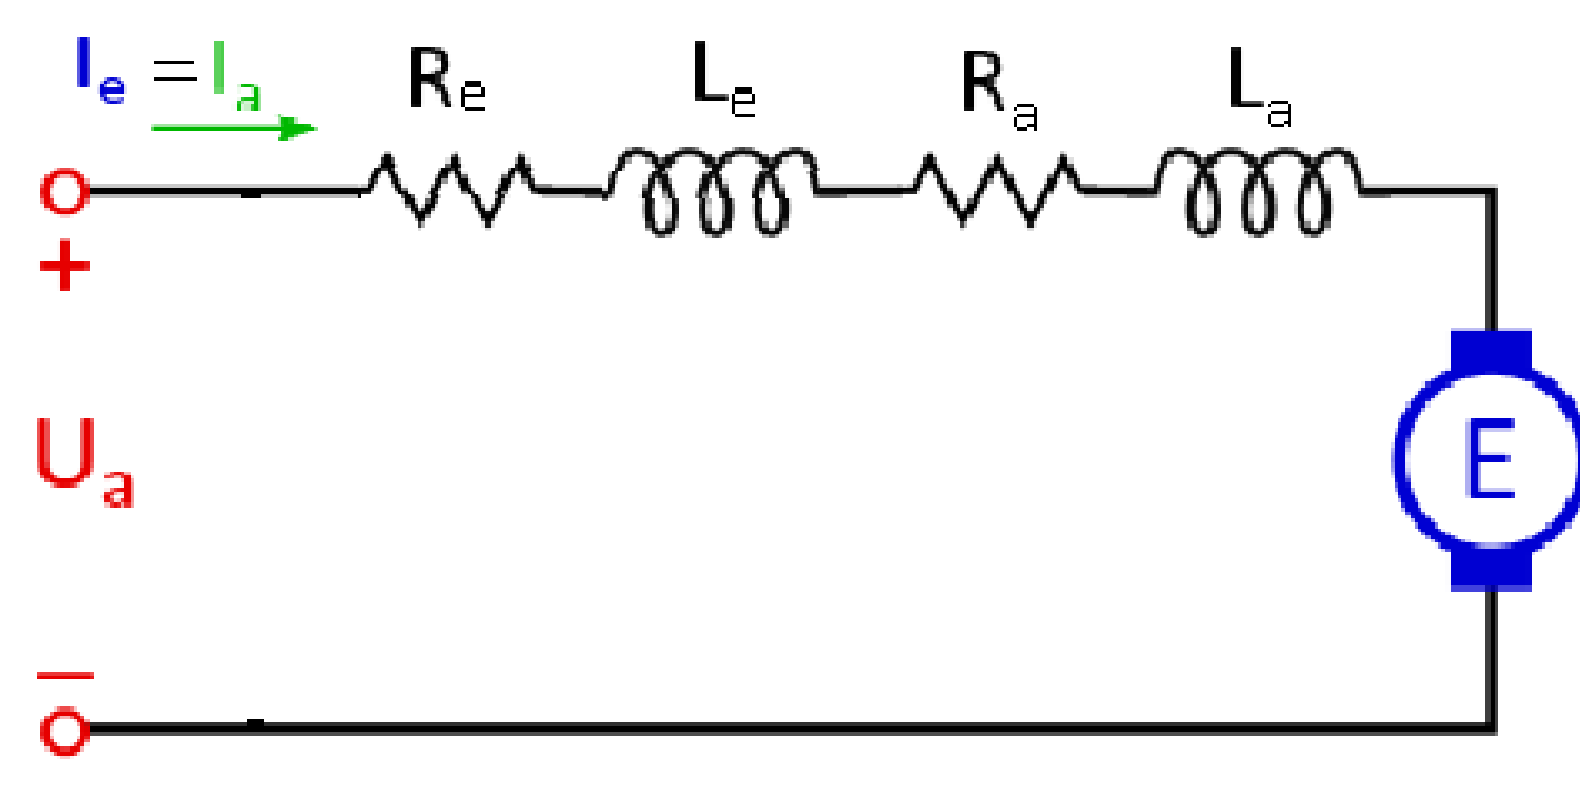
\includegraphics[width=0.6\textwidth]{assets/seriebekrachtiging.png}
     \caption{Serie bekrachtiging van een DC-machine}
     \label{fig:seriebekrachtiging.png}
    \end{figure}
\end{itemize}
Andere types motoren zijn:
\begin{itemize}
 \item \textbf{PMDC (Permanent Magnet DC)}: Deze zien we later nog in de cursus, dit is een DC-machine met permanente magneten in de rotor, dit is dus een synchrone machine. Deze heeft geen bekrachtiging nodig want de magneten zorgen voor het veld.
 \item \textbf{Compound}: Dit combineert de eigenschappen van zowel shunt- als serie-excitatie, waardoor het koppel en de snelheid beter gereguleerd kunnen worden. Het heeft zowel een parallelle als een seriële wikkeling. Deze motor komt weinig voor in de praktijk.
 \item \textbf{Borstelloze DC}: Zelfde T-n karakteristiek als een PMDC, maar de constructie lijkt op die van de synchrone machine.
\end{itemize}
\subsection{Karakteristieken}
\subsubsection{T-n karakteristiek}
\begin{warningbox}[Sommige delen hier zijn niet te vinden op de slides maar komen van lesnotities + AI]
  Na de volgende berekening voor T, is het deel van de grafieken vooral door AI gecooked op basis van mijn lesnotities, want dat deel staat niet in de slides ma kwam wel in de les aan bod dus ik waarschuw dat het misschien niet zo vlot leest als de rest en mogelijks fouten in kunnen staan, de grafieken kloppen wel normaal al zowieso wat denkik ook het belangrijkste is. Die getallen bij die grafieken, zoals je zult zien, zijn random en hebben geen betekenis.
\end{warningbox}
Met de eerder opgestelde vergelijkingen kunnen we de T-n karakteristiek van de DC-machine bepalen. We weten dat:
\begin{align*}
    T = C \cdot \varphi \cdot i_a
\end{align*}
En dat:
\begin{align*}
    U_a = E + R_a \cdot i_a
\end{align*}
Invullen voor $i_a$ geeft:
\begin{align*}
    T = C \cdot \varphi \cdot \frac{U_a - E}{R_a}
\end{align*}
En invullen voor E geeft:
\begin{align*}
    T = \frac{C \cdot \varphi \cdot U_a}{R_a} - \frac{C^2 \cdot \varphi^2 \cdot \omega}{R_a}
\end{align*}
Hierbij zijn $E$, $i_a$ en $\omega$ variabelen die kunnen veranderen en $R_a$ een parameter (constant).
\newline
\newline
{\color{red}Vanaf hier tot 'magnetisatiecurve' is het AI slop.}
\subsubsection{Aparte en shunt excitatie}
Bij aparte en shunt excitatie is het veld onafhankelijk van $i_a$, dus $\varphi \approx$ constant. Uit $T = C\varphi i_a$, $U_a = E + R_a i_a$ en $E = C\varphi\omega$ volgt de \textbf{lineaire} $T$-$\omega$ relatie:
\begin{align*}
    T = \frac{C \varphi U_a}{R_a} - \frac{C^2 \varphi^2}{R_a} \cdot \omega
\end{align*}

\begin{figure}[H]
\centering
\begin{tikzpicture}
\begin{axis}[xlabel={$n$}, ylabel={$T$}, xmin=0, xmax=10, ymin=0, ymax=11, axis lines=left, thick, domain=0:8, samples=50]
\addplot[blue] {10 - 1.25*x};
\end{axis}
\end{tikzpicture}
\caption{Kwalitatieve T-n karakteristiek bij aparte/shunt excitatie}
\end{figure}

\textbf{Snijpunten:} bij stilstand ($\omega=0$) is $E=0$, dus $i_{a,aanloop}=U_a/R_a$ (groot, want $R_a$ klein $\to$ aanloopweerstand nodig) en $T_{aanloop} = C\varphi U_a/R_a$. Bij onbelast ($T=0$) krijg je het nullasttoerental $\omega_0 = U_a/(C\varphi)$.

\subsubsection{Invloed van $U_a$ en $\varphi$ op de karakteristiek}
\textbf{$U_a$ aanpassen (aparte excitatie):} de helling $-C^2\varphi^2/R_a$ hangt niet af van $U_a$, dus je krijgt \textbf{parallelle rechten}: hogere $U_a$ $\to$ hoger $T_{aanloop}$ én hoger $\omega_0$, beide evenredig met $U_a$. Elke rechte heeft dus zijn eigen nulpunt (snelheid waar $T=0$) -- dit gebruikt men om de snelheid te regelen onder het nominale toerental.

\begin{figure}[H]
\centering
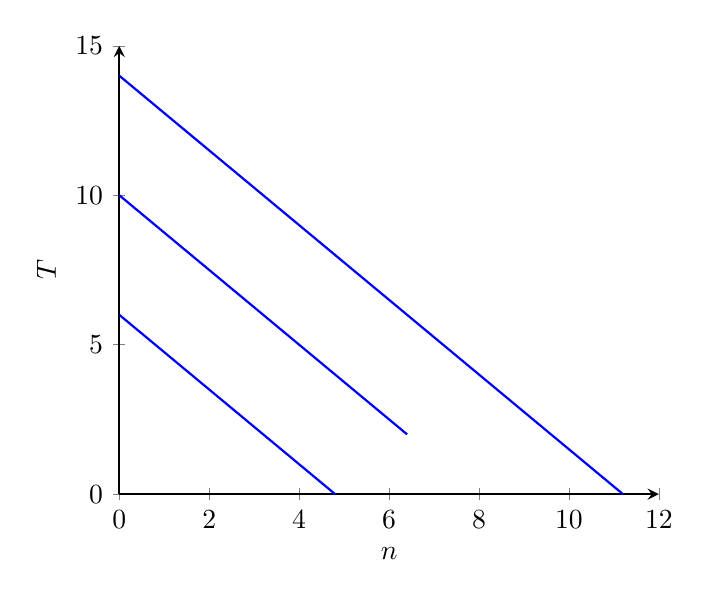
\begin{tikzpicture}
\begin{axis}[xlabel={$n$}, ylabel={$T$}, xmin=0, xmax=12, ymin=0, ymax=15, axis lines=left, thick]
\addplot[blue, domain=0:6.4, samples=50] {10 - 1.25*x};
\addplot[blue, domain=0:11.2, samples=50] {14 - 1.25*x};
\addplot[blue, domain=0:4.8, samples=50] {6 - 1.25*x};
\end{axis}
\end{tikzpicture}
\caption{Aanpassen van $U_a$ bij constante $\varphi$: parallelle rechten}
\end{figure}

\textbf{Let op bij shunt:} het veld hangt hier aan dezelfde voeding als het anker, dus als je $U_a$ aanpast verandert $i_e$ (en dus $\varphi$) mee -- de rechten zijn dan \textbf{niet} zuiver parallel.

\textbf{Veldverzwakking ($\varphi$ aanpassen bij constante $U_a$):} kleinere $\varphi$ geeft een \textbf{kleinere helling} (want $\varphi^2$ zit in de helling) $\to$ hoger $\omega_0$ maar lager $T_{aanloop}$. Dit gebruikt men om \textbf{boven} het nominale toerental te draaien, ten koste van koppel.

\begin{figure}[H]
\centering
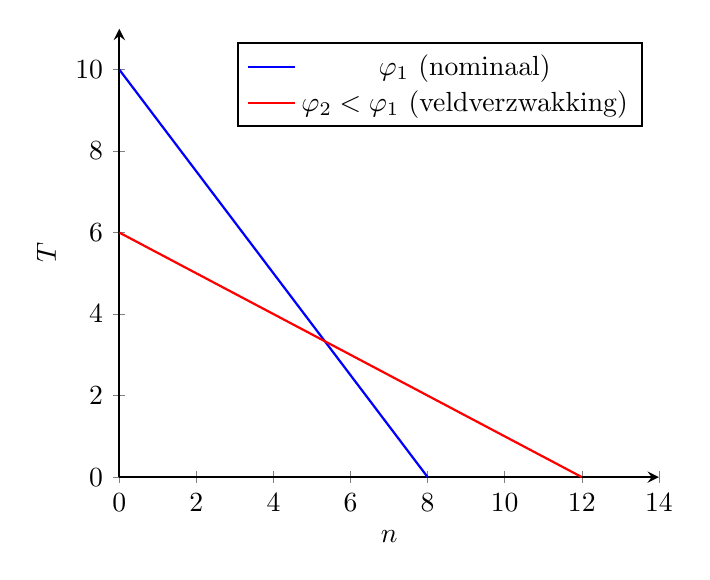
\begin{tikzpicture}
\begin{axis}[xlabel={$n$}, ylabel={$T$}, xmin=0, xmax=14, ymin=0, ymax=11, axis lines=left, thick, legend pos=north east]
\addplot[blue, domain=0:8, samples=50] {10 - 1.25*x};
\addlegendentry{$\varphi_1$ (nominaal)}
\addplot[red, domain=0:12, samples=50] {6 - 0.5*x};
\addlegendentry{$\varphi_2 < \varphi_1$ (veldverzwakking)}
\end{axis}
\end{tikzpicture}
\caption{Veldverzwakking: kleinere $\varphi$ geeft vlakkere rechte}
\end{figure}
\subsubsection{Serie excitatie}
Hier is $i_e = i_a$, hieruit volgt voor het koppel:
\begin{align*}
    T = G \cdot (\frac{U_a - E}{R_a})^2
\end{align*}
Dit is een \textbf{hyperboolachtige} curve, geen rechte.

\begin{figure}[H]
\centering
\begin{tikzpicture}
\begin{axis}[xlabel={$n$}, ylabel={$T$}, xmin=0, xmax=10, ymin=0, ymax=11, axis lines=left, thick, domain=0:10, samples=50]
\addplot[red] {10/((1+0.5*x)^2)};
\end{axis}
\end{tikzpicture}
\caption{Kwalitatieve T-n karakteristiek bij serie excitatie}
\end{figure}

\textbf{Belangrijk:} er is \textbf{geen} eindig nulpunt -- $\omega \to \infty$ als $T \to 0$. Een seriemotor mag dus \textbf{nooit onbelast draaien} (loopt op hol).

\subsubsection{Vergelijking}
\begin{figure}[H]
\centering
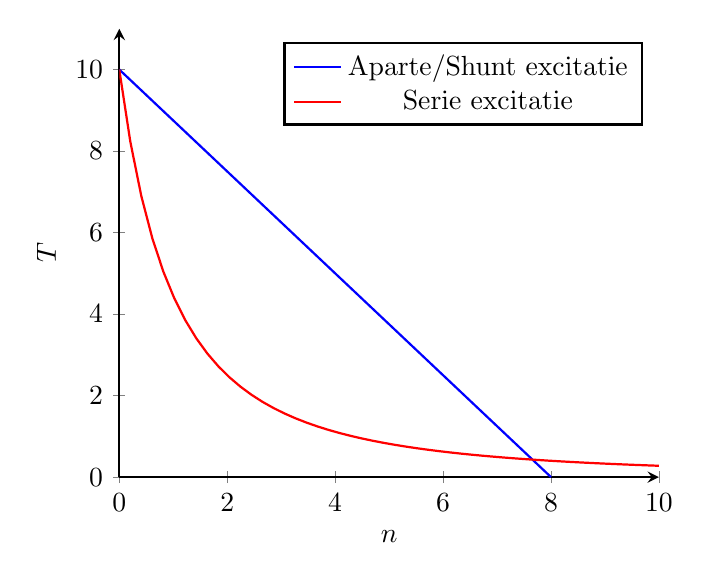
\begin{tikzpicture}
\begin{axis}[xlabel={$n$}, ylabel={$T$}, xmin=0, xmax=10, ymin=0, ymax=11, axis lines=left, thick, legend pos=north east]
\addplot[blue, domain=0:8, samples=50] {10 - 1.25*x};
\addlegendentry{Aparte/Shunt excitatie}
\addplot[red, domain=0:10, samples=50] {10/((1+0.5*x)^2)};
\addlegendentry{Serie excitatie}
\end{axis}
\end{tikzpicture}
\caption{Vergelijking van de T-n karakteristieken}
\end{figure}

\subsubsection{Constante ankerstroom}
Bij constante $i_a$ (en constante $\varphi$) is ook $T = C\varphi i_a$ constant, onafhankelijk van $n$. Omdat $E = C\varphi n$ een rechte door de oorsprong is, en $U_a = E + R_a i_a$ daar een parallelle rechte van is, blijft de horizontale afstand tussen $U_a$ en $E$ overal gelijk aan $R_a i_a$.

\begin{figure}[H]
\centering
\begin{tikzpicture}
    % Assen
    \draw[->] (0,0) -- (8,0) node[right] {$n$};
    \draw[->] (0,0) -- (0,7) node[above] {$T$};
    % Rode Ua-lijn: dalend, kruist n-as bij n_s
    \draw[red, thick] (0.3,6.5) -- (5,0);
    \node[red] at (0.6,7) {$U_a$ cte};
    % Blauwe E-lijn: verticaal, exact bij n_s
    \draw[blue, thick] (5,0) -- (5,6.5);
    \node[blue] at (5.4,7) {$E$ cte};
    \draw[dashed] (5,0) -- (5,-0.15);
    \node at (5,-0.4) {$n_s$};
    % Groene Ia-lijn: lager, los van Ua/E
    \draw[green!60!black, thick] (0,3) -- (7,3);
    \node[green!60!black] at (7.6,3) {$i_a$ cte};
    % Ra Ia pijl: HORIZONTAAL tussen rood en blauw, bovenaan
    \draw[<->, thick] (0.3,6.5) -- (5,6.5);
    \node at (2.65,6.8) {$R_a i_a$};
\end{tikzpicture}
\caption{Constante ankerstroom: horizontale afstand tussen $U_a$ en $E$ = $R_a i_a$; ze vallen samen bij $T=0$ (op $n_s$)}
\end{figure}
\subsection{Magnetisatiecurve}
Nog iets belangrijks om rekening mee te houden is magnetisatie: de flux $\varphi$ stijgt niet altijd lineair met de veldstroom $i_e$. Bij lage veldstromen is dit wel het geval, maar naarmate de veldstroom stijgt, treedt verzadiging op in het ijzer van de statorpolen. Hierdoor neemt $\varphi$ minder snel toe met $i_e$, wat op zijn beurt de T-n karakteristiek beïnvloedt. De veldwikkeling heeft dus eigenlijk een nominale stroom: voorbij die grens levert een hogere $i_e$ vooral opwarming in de spoelen op, want de veldsterkte $H$ blijft dan wel toenemen, maar $B$ (en dus $\varphi$) niet meer. De volgende grafiek toont deze magnetisatiecurve voor drie snelheidsgevallen ($N_3 > N_2 > N_1$), waarbij de veldstroom uitgezet is tegen de nullast-tegen-EMK (waar het koppel 0 is):
\begin{figure}[H]
  \centering
  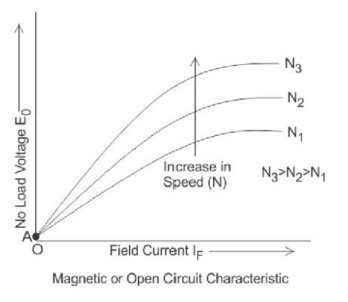
\includegraphics[width=0.5\textwidth]{assets/magnetisatiecurve.png}
  \caption{Magnetisatiecurve}
  \label{fig:magnetisatiecurve.png}
 \end{figure}
\newpage
\section{DC-motor problemen}
In het algemeen zijn er 3 problemen die kunnen optreden bij een DC-machine, deze zullen we nu bespreken.
\subsection{Open veld circuit}
Dit zegt eigenlijk dat het heel gevaarlijk is om het veld van de DC-machine 'open te zetten' (\textbf{onderbreken} eigenlijk). Ik herhaal hier nog even de 3 vergelijkingen van hierboven:
\begin{align*}
    U_a &= E + R_a i_a \\
    E &= C \cdot \varphi \cdot \omega \\
    T &= C \cdot \varphi \cdot i_a
\end{align*}
Stel dus dat we het circuit van dat veld onderbreken, dus $i_e$ wordt heel klein, waardoor het veld $\varphi$ ook heel klein wordt. In de praktijk daalt $\varphi$ echter nooit helemaal tot nul: door hysteresis in het ijzer blijft er een kleine \textbf{remanente flux} $\varphi_{rest}$ over, en die blijft hierna cruciaal. Op het moment dat het veld wegvalt, wordt het koppel $T$ eerst heel klein, maar op dat moment is de snelheid $\omega$ van de rotor nog steeds dezelfde en groot; ons tegen-emk wordt wel kleiner doordat het veld kleiner wordt. De klemspanning $U_a$ is constant, dus de volledige spanning gaat over dat $R_a \cdot i_a$ gedeelte staan, waardoor de stroom $i_a$ heel snel groot wordt en dus $R_a$ kan doorbranden (\textit{anker opbranden}). En omdat $i_a$ zo snel zo groot wordt, zorgt zelfs die kleine restflux $\varphi_{rest}$ voor een aanzienlijk koppel ($T=C\varphi_{rest} i_a$), waardoor de snelheid $\omega$ ook heel groot gaat worden -- de snelheid gaat dus eigenlijk naar oneindig. Dit is dus een gevaarlijke situatie, en daarom mag je het veld van een DC-machine nooit open zetten.
\subsection{Commutator arcing (borstelvuur/vonken)}
We weten nu al dat de commutator uit veel aparte stukken bestaat, en dat de koolstofborstels daar tegenaan drukken. Terwijl de rotor draait, moet elke spoel op een bepaald moment van polariteit wisselen: de borstel raakt dan heel even twee naburige commutatorlamellen tegelijk en sluit die spoel kort, waarbij de stroom moet omkeren van $+i$ naar $-i$. Omdat elke spoel een zelfinductie $L$ heeft, verzet ze zich tegen die snelle stroomverandering via:
\begin{align*}
    u_L = L \cdot \frac{di}{dt}
\end{align*}
Omdat de omkering in een heel korte commutatieperiode moet gebeuren, is $di/dt$ groot, en dus ook $u_L$. Net op het moment dat het koperoppervlak van de lamel onder de borstel verdwijnt, wil de stroom door die inductie nog blijven vloeien -- ze springt dan over het luchtspleetje tussen borstel en lamel, ioniseert de lucht, en er ontstaat een vonk. Die vonken vreten zowel de koolstofborstel als de lamellen weg, en bij hevige/chronische vonkvorming kan dit escaleren tot \textbf{borstelvuur} (ringvuur): een doorlopende boog over meerdere lamellen die de machine zwaar kan beschadigen.

Om dit te beperken gebruikt men \textbf{commutatiepolen} (hulppolen die $u_L$ compenseren), plaatst men de borstels op het \textbf{neutrale vlak}, en gebruikt men \textbf{koolstof} als borstelmateriaal voor een geleidelijkere weerstandscommutatie. 
\newline
\newline
Dit is dus wel iets dat voorkomt bij snelle snelheden, de snelheid beperken kan dus ook dit effect verminderen.
\newpage
\subsection{Ankerreactie}
Een ander probleem dat kan optreden is de ankerreactie, dit is eigelijk \textbf{het effect van het veld van de rotor op het veld van de stator}, het vervormt het veld van de stator dus. Dit is wat we eerder zagen, de wet van Ampère zegt dat een stroomvoerende geleider een magnetisch veld opwekt, en de rotor is dus een stroomvoerende geleider. Dit zorgt voor een fluxverlies, en dat het 'neutrale vlak' gaat draaien, dit zien we in de volgende figuur:
\begin{figure}[H]
  \centering
  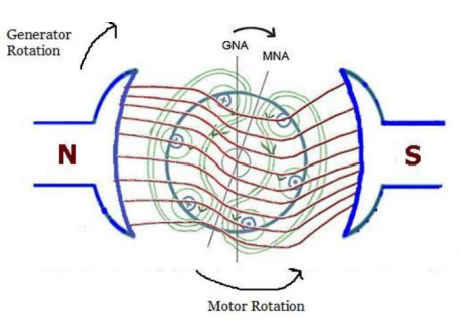
\includegraphics[width=0.5\textwidth]{assets/ankerreactie.png}
  \caption{Ankerreactie}
  \label{fig:ankerreactie.png}
 \end{figure}
Het 'neutrale vlak' (aangeduid met GNA) is het vlak waar de stroom door de rotor loodrecht staat op het veld van de stator, en dus geen tegen-emk induceert. Door de ankerreactie wordt dit vlak verschoven (aangeduid met MNA (modified)), waardoor de commutatie niet meer optimaal is en er vonkvorming kan optreden. Dit effect kan worden verminderd door het gebruik van commutatiepolen en door de juiste plaatsing van de koolstofborstels (schuin dus, hoeveel hangt af van de stroom). Er zijn dus trucjes om dit op te lossen maar dat moeten we niet kennen.
\newpage
\section{DC-motor oefeningen}
\begin{oefenblok}[Oefening 1 (Op slides)]
\textbf{Opgave:}
\newline
A shunt-connected 75kW, 250V DC motor has an armature resistance of 45mohm and a field resistance of 185ohm. When operated at 250V its no-load speed is 1850rpm. The motor is operating under load at a terminal voltage of 250V and a terminal current of 290A.
\begin{itemize}
  \item a) Calculate the motor speed, load power, load torque in this operation point.
  \item b) Assuming the load torque remains constant as a function of speed, calculate the motor speed if the terminal voltage is reduced to 200V.
\end{itemize}
\textbf{Oplossing:}
\newline
We schrijven eerst eens rap onze gegevens op: 
\begin{itemize}
 \item $P = 75 kW$
 \item $U_a = 250 V$
 \item $R_a = 45 m\Omega$
 \item $R_{veld} = 185 \Omega$
 \item $n_{no,load} = 1850 rpm$
 \item $I = 290 A$
\end{itemize}
Teken altijd een schema van het circuit van de motor! Hier is het shunt bekrachtigd, dus de opstelling, met al gegevens ingevuld ziet er zo uit:
\begin{figure}[H]
  \centering
  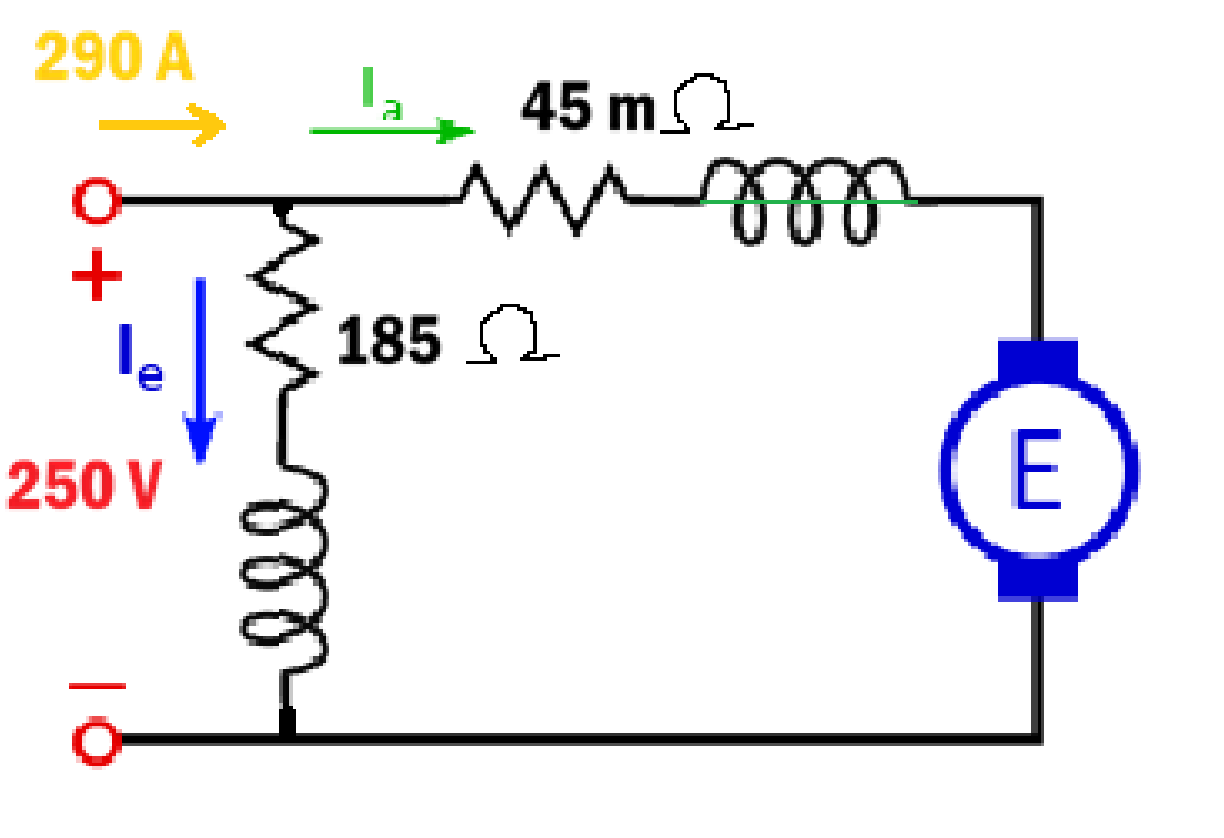
\includegraphics[width=0.5\textwidth]{assets/schemaoef1dc.png}
  \caption{Schema van de shunt-connected DC-motor Oefening 1}
  \label{fig:schemaoef1dc.png}
 \end{figure}
De spoel van rotor ($L_a$) is daar doorgetrokken met een groene lijn, we negeren deze want de spanningsval hierover is zo goed als 0.
\newline
\newline
De snelheid van de motor kunnen we berekenen met de eerder gezien formule van het tegen-emk:
\begin{align*}
    E = C \cdot \varphi \cdot \omega
\end{align*}
We hebben $C \cdot \varphi$ niet, maar we kunnen dit wel berekenen met de gegevens van de no-load situatie, want hier is $E_0 = U_a - R_a \cdot I_a$ maar bij no-load is $I_a = 0$:
\begin{align*}
    C \cdot \varphi = \frac{E_0}{\omega} = \frac{U_a}{2 \pi n_{no,load}/60} = \frac{250}{2 \pi \cdot 1850/60} = 1.29 Vs
\end{align*}
We kunnen ook de veldstroom berekenen, want met deze stroom vinden we de ankerstroom:
\begin{align*}
    I_{veld} = \frac{U_a}{R_{veld}} = \frac{250}{185} = 1.35 A
\end{align*}
We kunnen nu de ankerstroom berekenen:
\begin{align*}
    I_a = I - I_{veld} = 290 - 1.35 = 288.65 A
\end{align*}
En met dit vinden we de tegen-emk van de motor:
\begin{align*}
    E = U_a - R_a \cdot I_a = 250 - 0.045 \cdot 288.65 = 237.01 V
\end{align*}
Dit invullen in de formule van het tegen-emk geeft ons de snelheid van de motor:
\begin{align*}
    n = \frac{E}{C \cdot \varphi} \cdot \frac{60}{2 \pi} = \frac{237.01}{1.29} \cdot \frac{60}{2 \pi} = 1753.5 rpm
\end{align*}
Het vermogen van de motor kunnen we berekenen met de formule:
\begin{align*}
    P_{last} = T \cdot \omega = T \cdot \frac{2 \pi n}{60}
\end{align*}
We hebben $T$ niet, maar we kunnen dit wel berekenen met de formule van het koppel:
\begin{align*}
    T = C \cdot \varphi \cdot I_a = 1.29 \cdot 288.65 = 372.2 Nm
\end{align*}
Invullen in de formule van het vermogen geeft ons:
\begin{align*}
    P_{last} = 372.2 \cdot \frac{2 \pi \cdot 1753.5}{60} = 68000 W = 68 kW
\end{align*}
\textbf{Deel b van de oefening:}
\newline
Nu daalt de klemspanning naar 200V, maar het koppel blijft constant, dus die $T = 372.2 Nm$ blijft behouden. Doordat de spanning daalt, zal de veldstroom dalen naar:
\begin{align*}
    I_{veld} = \frac{U_a}{R_{veld}} = \frac{200}{185} = 1.08 A
\end{align*}
De totale stroom zal ook veranderen, maar nu dat we weten dat het koppel constant blijft, kunnen we de ankerstroom berekenen. Dit doen we met:
\begin{align*}
    T = I_{a,2} \cdot C \cdot \varphi_2
\end{align*}
De factor $C \cdot \varphi_2$ kunnen we berekenen terug met de nullast situatie maar nu met een klemspanning van 200V:
\begin{align*}
    C \cdot \varphi_2 = \frac{E_0}{\omega} = \frac{U_a}{2 \pi n_{no,load}/60} = \frac{200}{2 \pi \cdot 1850/60} = 1.03 Vs
\end{align*}
Invullen in de formule van het koppel geeft ons:
\begin{align*}
    I_{a,2} = \frac{T}{C \cdot \varphi_2} = \frac{372.2}{1.03} = 361.5
\end{align*}
We kunnen nu de tegen-emk berekenen:
\begin{align*}
    E_2 = U_a - R_a \cdot I_{a,2} = 200 - 0.045 \cdot 361.5 = 183.7 V
\end{align*}
En met dit vinden we de snelheid van de motor:
\begin{align*}
    n_2 = \frac{E_2}{C \cdot \varphi_2} \cdot \frac{60}{2 \pi} = \frac{183.7}{1.03} \cdot \frac{60}{2 \pi} = 1703.5 rpm
\end{align*}
\end{oefenblok}
Volgende oefening staat niet in de slides, maar wel op toledo. Ik raad zeker aan deze te maken aangezien het grote deel van het examen op oefeningen telt terwijl er geen oefensessies van dit vak zijn.
\begin{oefenblok}[Oefening 2 (Op Toledo)]
\textbf{Opgave:}
\newline
A four-pole, 25kW , 250V separately excited DC motor is mechanically coupled to a threephase four-pole, 25kW, 460V, cylindrical pole synchronous generator. The DC motor is connected to a constant 250V DC supply and the ac generator is connected to a 460V fixed voltage, fixed frequency, threephase grid. The synchronous reactance of the synchroous generator is 6.6 $\Omega$. The armature resistance of the DC motor is 22 $m\Omega$. All unspecified losses are to be neglected.
\begin{itemize}
 \item 1) If the two machines act as a motor-generator set receiving power from the DC source and delivering power to the ac grid, what is the internal phase voltage ESM of the ac machine when it delivers 25kW at unity power factor? What is the internal voltage (back-emf) of the DC motor?
 \item 2) Leaving the field current of the ac machine at the value corresponding to the condition of part (a), what adjustment can be made to reduce the power transfer between the two machines to zero? Under this condition of zero power transfer, what is the armature current of the DC machine? What is the armature current of the ac machine?
 \item 3) Leaving the field current of the ac machine as in parts (a) and (b), what adjustment can be made to cause the transfer of 25kW from tha ac source to the DC source? Under these conditions, what are the armature current and internal voltage of the DC machine? What will be the magnitude and phase of the current in the ac machine?
\end{itemize}
\textbf{Oplossing:}
\dots ({\color{red}Nog niet aan begonnen})
\end{oefenblok}
\newpage
\chapter{Draaiveld}
We weten nu dus dat we een statorveld hebben, we gaan nu kijken naar hoe we deze gaan opwekken en hoe we dit kunnen gebruiken om een rotor te laten draaien. Even ter verduidelijking ook, de rotor heeft dus ook een magnetisch veld en dat was degene met een constant magnetisch veld, maar de stator heeft een \textbf{draaiveld} (rotating field). Dit is een magnetisch veld dat in de ruimte draait.
\begin{figure}[H]
  \centering
  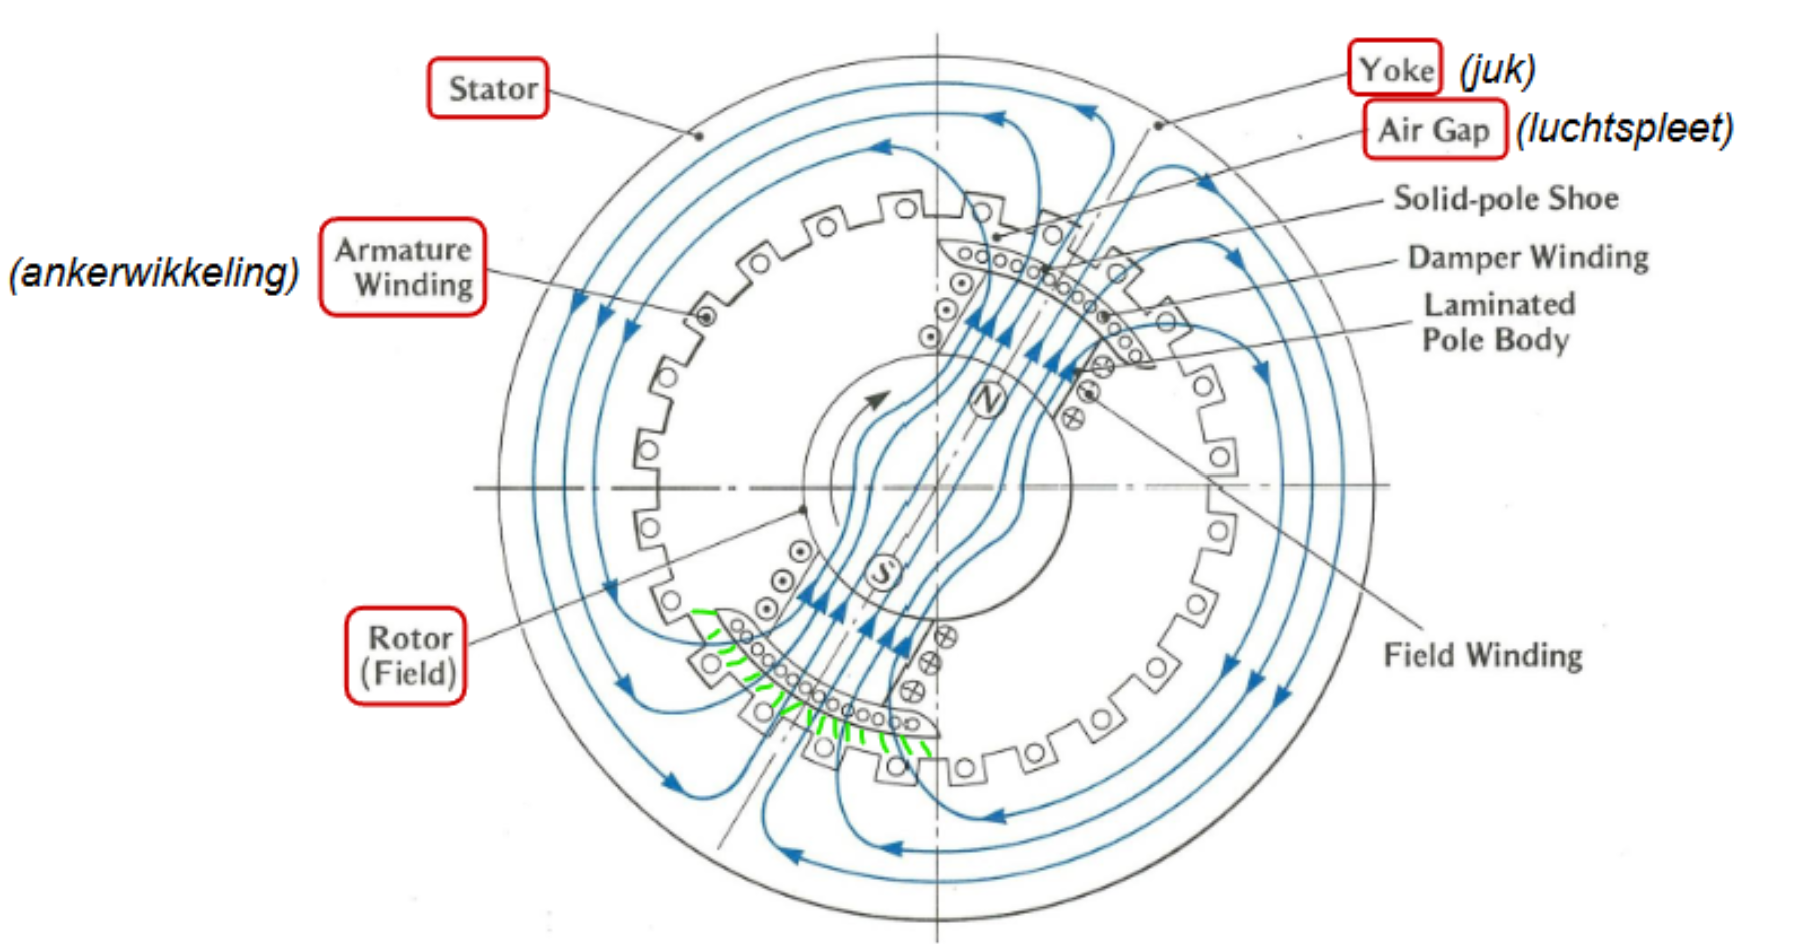
\includegraphics[width=0.7\textwidth]{assets/weergavemagnetischveldinmotor.png}
  \caption{Magnetisch veld in een motor}
  \label{fig:weergavemagnetischveldinmotor.png}
 \end{figure}
Tussen de stator en de rotor is er dus een \textbf{luchtspleet}, typisch 0,5 tot 1mm groot, in de figuur hierboven is deels van die luchtspleet aangeduid in het groen. Het magnetisch veld van de stator gaat hierdoor om tot de rotor te geraken en het rotor veld het stator veld te doen volgen maar dit zien we zometeen. De 'Yoke' of \textbf{juk} is waar de veldlijnen 'terugkeren' langs de achterkant, wat je je een beetje kan inbeelden door naar deze figuur te zien.
\newline
\newline
We veronderstellen nu dat onze rotor een mooie ronde ijzeren cilinder is, dit maakt het meer symmetrisch en maakt dat onze analyse die we nu gaan doen volledig correct is. We kijken even naar 1 van die wikkelingen, deze is dan gesitueerd in die statorgleuven zoals in de volgende figuur:
\begin{figure}[H]
  \centering
  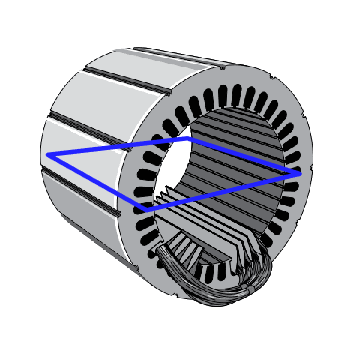
\includegraphics[width=0.4\textwidth]{assets/1wikkelinginstator.png}
  \caption{1 wikkeling in stator}
  \label{fig:1wikkelinginstator.png}
 \end{figure}
\newpage
Als we nu door deze éne wikkeling een wisselstroom sturen, dan zal er door die wikkeling ook een wisselveld ontstaan, dit is een magnetisch veld dat in de ruimte oscilleert, op en neer eigelijk zoals in deze figuur:
\begin{figure}[H]
  \centering
  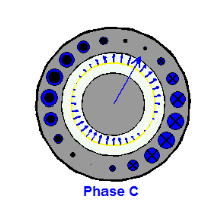
\includegraphics[width=0.4\textwidth]{assets/1wikkelingwisselveld.png}
  \caption{1 wikkeling met wisselveld}
  \label{fig:1wikkelingwisselveld.png}
 \end{figure}
Hier staat het wel een beetje schuin onder een hoek, de animatie hiervan staat gewoon op toledo je kan die daar bezien. Die gele lijn is de luchtspleet, het is vanaf hier dat de magnetische veld vectoren getekend worden. We zijn vooral geinteresseerd in die luchtspleet want hier gaat het over van stator naar rotor, zo wordt het koppel opgewekt. Als we nu 2 andere wikkelingen plaatsen, die elk 120° van elkaar verwijderd zijn, en we sturen door elk van deze wikkelingen een wisselstroom die 120° van elkaar verschoven is, dan zal er een \textbf{draaiveld} ontstaan. 
\begin{figure}[H]
  \centering
  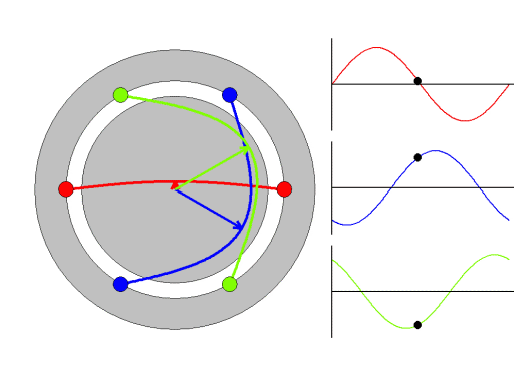
\includegraphics[width=0.5\textwidth]{assets/draaiveld3wikkelingen.png}
  \caption{Draaiveld met 3 wikkelingen}
  \label{fig:draaiveld3wikkelingen.png}
 \end{figure}
Dit is dus ook eigelijk een animatie, waarin die linkse figuur eigelijk die golven alle 3 op en neer gaan en het doet lijken dat het draait (dat doet het ook), check gewoon op toledo naar deze animatie als je het niet snapt. Dit kan ook zo weergegeven worden, hierbij draait die roze pijl gewoon tegenwijzerzin, heel die figuur eigelijk, voor de rest veranderd er niks:
\begin{figure}[H]
  \centering
  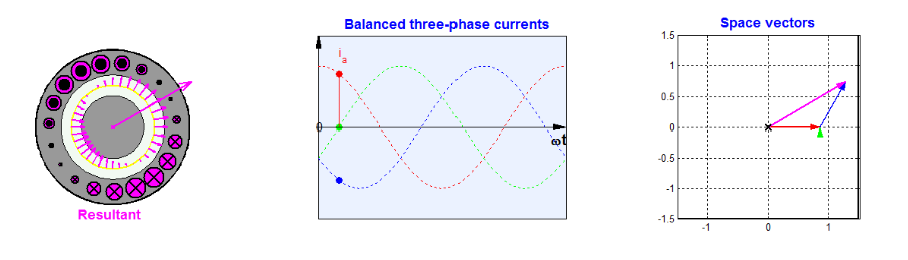
\includegraphics[width=0.8\textwidth]{assets/resulterendedraaiveld.png}
  \caption{Resulterend draaiveld}
  \label{fig:resulterendedraaiveld.png}
 \end{figure}
% Inhoud volgt
Zo een stroom zorgt dus voor een wisselveld, we kunnen deze 3 wisselvelden beschrijven afhankelijk van hun \textbf{hoekpositie} in de ruimte en hun \textbf{tijdspositie (faseverschuiving)}, deze gaan in de vorm van de uitdrukking van de \textbf{staande golf} staan:
\begin{align*}
    B_a(t, \alpha) = \hat{B}_{a} \cdot \sin(\omega_s \cdot t) \cdot \cos(\alpha) \\
    B_b(t, \alpha) = \hat{B}_{b} \cdot \sin(\omega_s \cdot t - 2\pi/3) \cdot \cos(\alpha - 2\pi/3) \\
    B_c(t, \alpha) = \hat{B}_{c} \cdot \sin(\omega_s \cdot t - 4\pi/3) \cdot \cos(\alpha - 4\pi/3)
\end{align*}
Het is dat sinus gedeelte dat de faseverschuiving (tijd) voorstelt en het cosinus gedeelte de hoekpositie (geometrisch). Het zijn dus ook deze 3 velden die samen het resulterende draaiveld vormen.
\begin{warningbox}[Faseverschuiving tussen die stromen is belangrijk!]
  Als er door die 3 wikkelingen dezelfde stromen met dezelfde faseverschuiving gaan dan krijg je een resulterend veld van 0! Het is de verschillende faseverschuivingen dat ervoor zorgen dat je resulterend veld niet 0 is. Ook belangrijk te onthouden is dat het resulterend veld dan \textit{geen} wisselveld is, maar een \textit{draaiveld}
\end{warningbox}
Het draaiveld heeft een bepaalde snelheid, de \textbf{pulsatie}, dit is een \textbf{elektrische snelheid!} Deze wordt gegeven door:
\begin{align*}
    \omega_s = 2 \pi f
\end{align*}
Het toerental in deze elektrische vorm wordt gegeven door:
\begin{align*}
    n_s = 60 \cdot f
\end{align*}
En eigelijk is die $\alpha$ in die uitdrukkingen van hierboven een geometrische (mechanische) hoekpositie, maar we hebben ook een elektrische hoekpositie $\theta_{se}$, dit is eigelijk de faseverschuiving. Het bepalen van deze hoek wordt gedaan met:
\begin{align*}
    \theta_{se} = p \cdot \theta_{sm} = p \cdot \alpha
\end{align*}
Die $\theta_{sm}$ is gewoon die $\alpha$, het kwam gewoon voor in de les dus ik zeg het maar zodat je niet verward wordt. Die p is dus het \textbf{poolpaartal}.
\subsection{Poolpaartal}
Wat is nu het poolpaartal effectief? Wat is de invloed van de hoeveelheid polen? Dit is belangrijk om naar te zien want deze machines hebben niet gewoon 3 wikkelingen zoals we eerder zagen, maar hebben in de praktijk meerdere draden dat door de gleuven van de stator gaan. En afhankelijk van hoe je deze draden positioneert kan je een bepaald aantal polen creëren. In de volgende figuur zie je dat:
\begin{figure}[H]
  \centering
  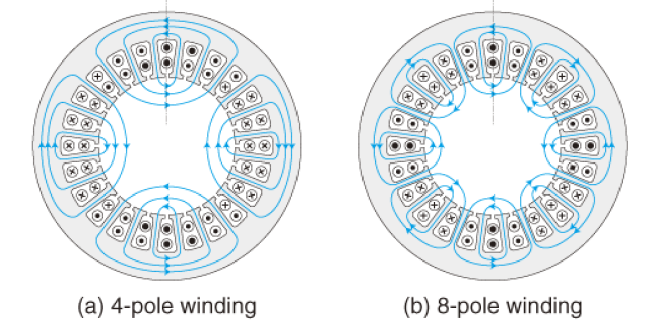
\includegraphics[width=0.6\textwidth]{assets/verschillendepolenevenveeldraden.png}
  \caption{Zelfde constructie met andere polen}
  \label{fig:verschillendepolenevenveeldraden.png}
 \end{figure}
In de industrie gaan we meestal machines met 4 polen (P=4) gebruiken, dus een poolpaartal p van 2 ($p = \frac{P}{2}$), het poolpaartal is dus het aantal koppels van noord- en zuidpolen dat een motor heeft. Hoe meer polen we willen, hoe grotere diameter je echter wel gaat nodig hebben want de positie van die wikkelingen is voor grotere polen niet voldoende. Hoe meer polen we hebben hoe lager het toerental van de machine zal zijn, want het toerental wordt gegeven door:
\begin{align*}
    n_s = \frac{60 \cdot f}{p}
\end{align*}
Of
\begin{align*}
    \omega_s = \frac{2 \pi f}{p}
\end{align*}
Dit is dus de \textbf{synchrone snelheid} van de machine (met f de frequentie van het net), dit is de \textbf{mechanische snelheid} van het draaiveld (in de luchtspleet).
\begin{warningbox}[Niet te verwarren met de pulsatie!]
  De pulsatie $\omega_s$ is een \textbf{elektrische snelheid}, de synchrone snelheid $\omega_s$ is een \textbf{mechanische snelheid}. De pulsatie wordt gebruikt in de uitdrukkingen van het draaiveld, de synchrone snelheid wordt gebruikt om het toerental van de rotor te berekenen.\textbf{ Het is dus hetzelfde symbool maar betekent iets anders!}
\end{warningbox}
\subsection{Draaizin van de motor}
Bij een DC-machine is de draaizin omkeren doenbaar door de polariteit van de voeding om te keren.
\begin{align*}
  U_a = R_a \cdot i_a + E \\
  E = C \cdot \varphi \cdot \omega \\
\end{align*}
Dus die $\omega$ kan je omkeren door de polariteit van $U_a$ om te keren.
\newline
\newline
Bij een AC-machine heb je 3 fasen, hierbij kan je de draaizin omkeren door 2 van de 3 fasen om te wisselen.
\subsubsection{Kenplaat}
Op de kenplaat wordt zo goed als altijd de synchrone snelheid gegeven, het staat er gewoon in toeren per minuut maar je moet dus weten dat dit de synchrone snelheid is. Het poolpaartal kan je hiermee dan vinden want de frequentie waarop de machine werkt wordt ook gegeven. Vaak wordt ook oftewel de arbeidsfactor $\cos(\varphi)$ of het rendement $\eta$ gegeven, niet beide, want de ene kan van de andere afgeleid worden.
\subsection{Geïnduceerde spanning}
We gaan nu kijken naar de spanning die in de rotor wordt opgewekt door het draaiveld van de stator. We gaan dit doen door één wikkeling te bekijken die stil staat, maar waar het veld van de stator langs draait, en ook dat het veld mooi sinusoïdaal verspreid is. We gaan dus kijken naar de \textbf{bewegingsspanning} die in deze wikkeling wordt opgewekt.
\newline
\newline
We vertrekken van het draaiveld in de luchtspleet:
\begin{align*}
    B(t,\alpha) = \hat{B} \cdot \cos(\omega_s t - p\alpha)
\end{align*}
Onze opstelling ziet er zo uit:
\begin{figure}[H]
  \centering
  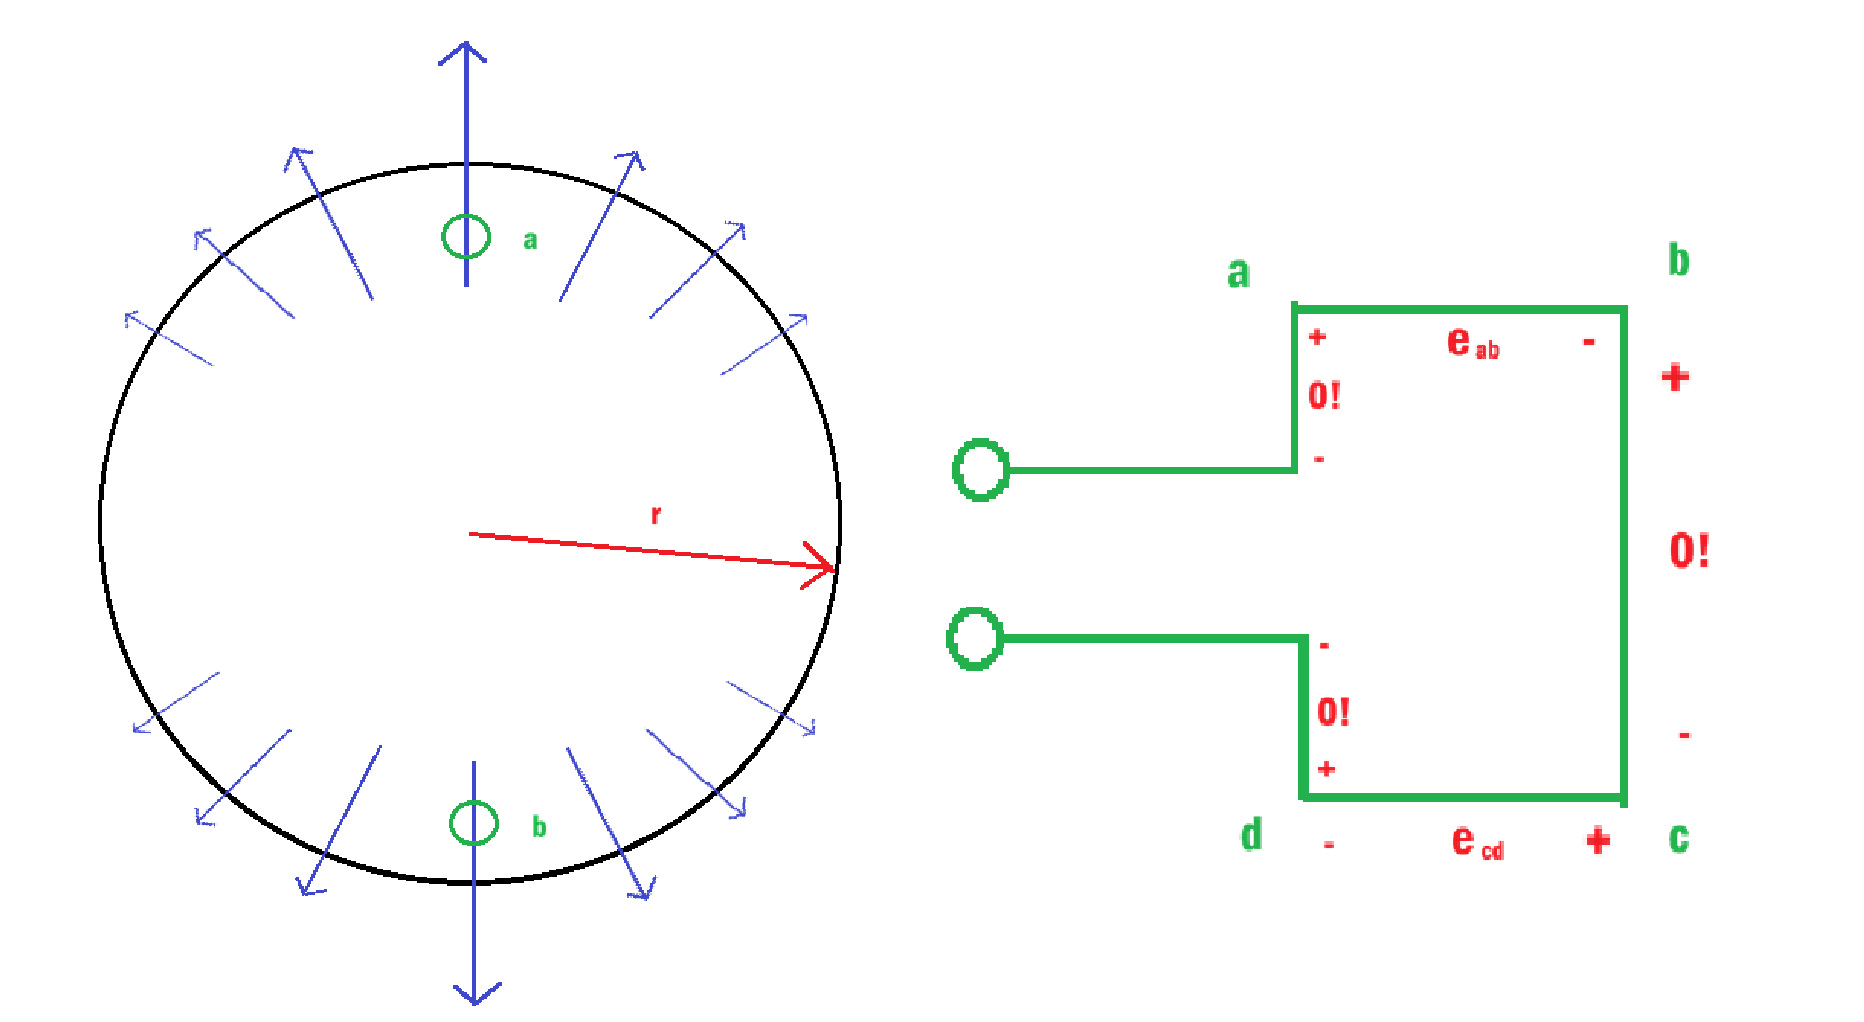
\includegraphics[width=0.6\textwidth]{assets/opstellingwikkelinggeinduceerdespanning.png}
  \caption{Opstelling}
  \label{fig:opstellingwikkelinggeinduceerdespanning.png}
 \end{figure}
Een stator­wikkeling staat stil, maar het veld draait er wel voorbij -- vanuit het perspectief van de geleider is dat equivalent aan een geleider die door een stilstaand veld beweegt (relatieve snelheid). We gebruiken dus de bewegingsspanning $e = B \cdot l \cdot v_{rel}$, met $v_{rel} = r \cdot \omega_s$ (r = straal, $\omega_s$ = synchrone snelheid), en alle parameters hier loodrecht op elkaar.

Voor geleider $ab$ (op positie $\alpha = 0$, het draaiveld draait tegenwijzerzin trouwens en we gaan van een poolpaar $p=1$ uit) geldt:
\begin{align*}
    e_{ab} = B \cdot |ab| \cdot v_{rel} = \hat{B}\cos(\omega_s t - p\alpha) \cdot |ab| \cdot r\omega_s = \hat{B} \cdot |ab| \cdot r\omega_s \cdot \cos(\omega_s t)
\end{align*}
De diametraal tegenoverliggende geleider $c$-$d$ zit een halve omwenteling verder ($\alpha \to \alpha - \pi$), maar door de supplementaire hoek levert dit exact dezelfde bijdrage, hij beweegt in de andere richting:
\begin{align*}
    e_{cd} = - \hat{B} \cdot |ab| \cdot r\omega_s \cdot \cos(\omega_s t - 1 \cdot \pi) = \hat{B} \cdot |ab| \cdot r\omega_s \cdot \cos(\omega_s t)
\end{align*}
De zijdes $e_{ad}$ en $e_{bc}$ leveren geen bijdrage, want ze bewegen parallel aan het veld.
\newline
\newline
De andere zijden van de spoel die we dus net bepaald hebben liggen in serie en versterken elkaar, dus voor \'e\'en winding:
\begin{align*}
    e_{ab-cd} = e_{tot} = 2\hat{B}|ab| \cdot r\omega_s \cos(\omega_s t)
\end{align*}
Met $N$ windingen en de flux per winding $\hat{\Phi}$ (die de $2\hat{B}|ab|r$-term bundelt) wordt dit:
\begin{align*}
    \boxed{e_a = N \hat{\Phi} \, \omega_s \cos(\omega_s t)}
\end{align*}

De drie fasewikkelingen liggen elk $120°$ uit elkaar rond de omtrek, wat zich vertaalt naar een elektrische faseverschuiving in de tijd:
\begin{align*}
    e_a &= N \hat{\Phi} \, \omega_s \cos(\omega_s t) \\
    e_b &= N \hat{\Phi} \, \omega_s \cos(\omega_s t - 120°) \\
    e_c &= N \hat{\Phi} \, \omega_s \cos(\omega_s t - 240°)
\end{align*}
Let op: dit is de \textbf{elektrische} hoek, niet de geometrische -- bij $p$ poolparen is de elektrische hoek $p$ keer de geometrische hoek, het hoedje op de flux, betekent dat het gaat om de piek waarde.
\newline
\newline
De effectieve (RMS) waarde volgt uit de amplitude gedeeld door $\sqrt{2}$ (met $\omega_s = 2\pi f$):
\begin{align*}
    E = \frac{N\hat{\Phi}\cdot 2\pi f}{\sqrt{2}} = \boxed{\sqrt{2}\,\pi \, f \, N \, \hat{\Phi}}
\end{align*}
\newpage
\subsection{Opgewekte koppel}
{\color{red}(Komend stukje is vooral door AI laten cooken want er zijn meerdere afleidingen hiervan gezien en ze zijn redelijk complex, heb ook geen idee of de afleidingen te kennen zijn)}
\newline
\newline
Met de wet van Lorentz kunnen we het opgewekte koppel berekenen.
\begin{figure}[H]
  \centering
  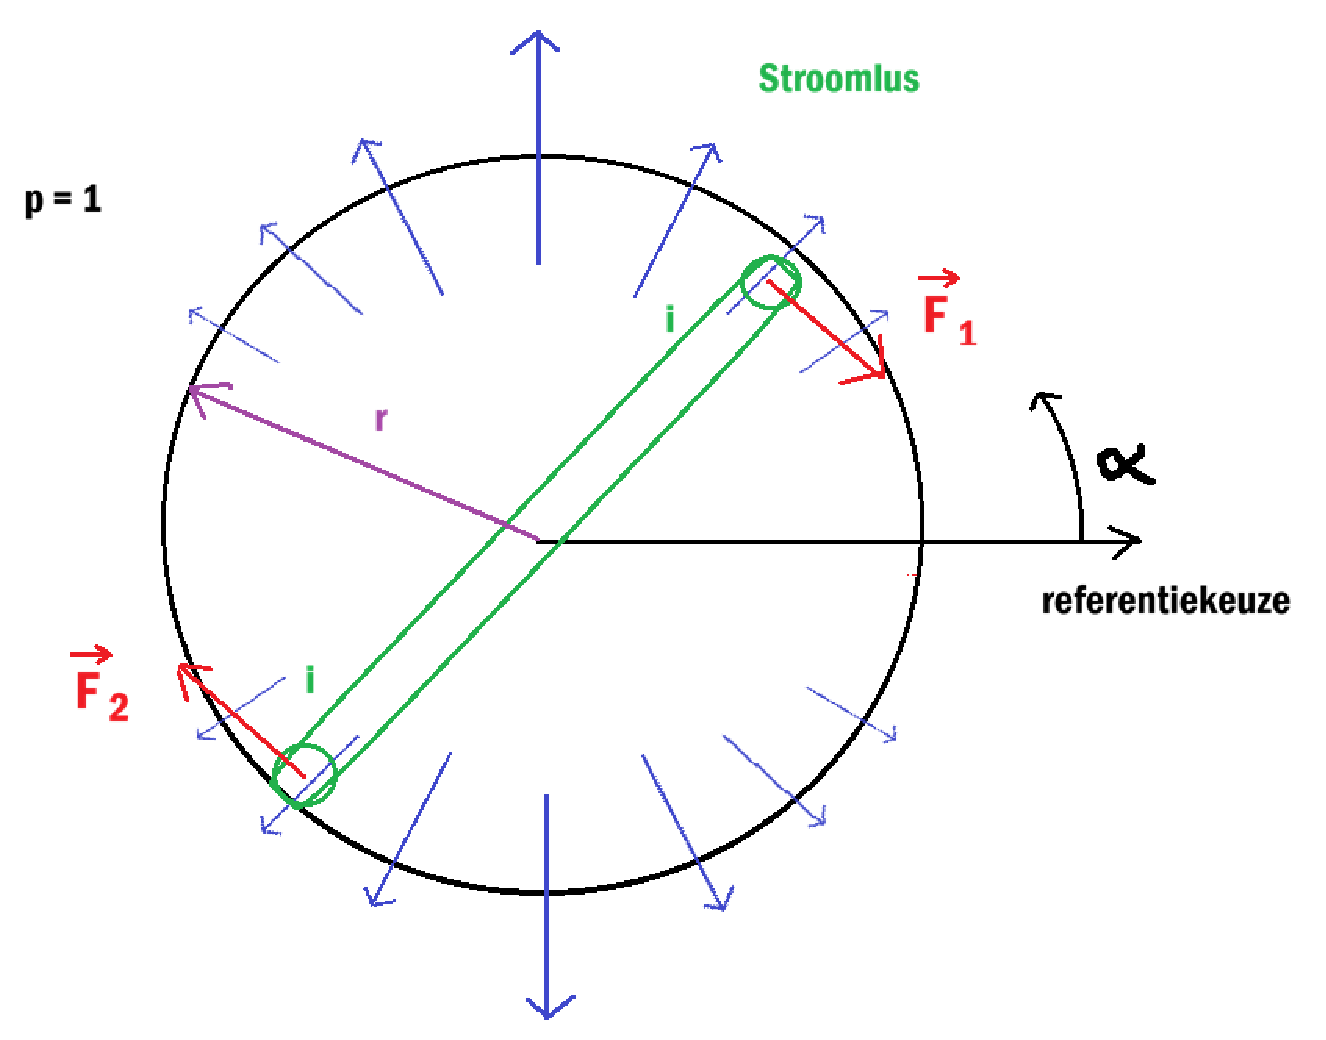
\includegraphics[width=0.5\textwidth]{assets/opstellingopgewektkoppel.png}
  \caption{Opstelling, hier is de lus onder een hoek, dit boeit in principe niet}
  \label{fig:opstellingopgewektkoppel.png}
 \end{figure}
De kracht op een geleider in een magnetisch veld is $F = B \cdot I \cdot l$, en het koppel is $T = F \cdot r$. Voor een rotor met $N$ geleiders en een flux $\Phi$ per poolpaar, wordt het totale koppel:
\begin{align*}
    F &= B_{\alpha} \cdot |ab| \cdot i_a \\
    &= \hat{B} \cos(\omega_s t - p\alpha) \cdot |ab| \cdot i_a
\end{align*}
Op $t=0$ (de Lorentzkracht bevat zelf geen tijdsafhankelijkheid, we bekijken dus een momentopname) en met $p=1$ vereenvoudigt dit tot:
\begin{align*}
    F = \hat{B} \cos\alpha \cdot |ab| \cdot i_a
\end{align*}
Deze kracht werkt op beide zijden van de wikkeling (diametraal tegenover elkaar op straal $r$), die samen een krachtenkoppel vormen. Voor $N$ windingen wordt het totale koppel dan:
\begin{align*}
    T = N \cdot F \cdot 2r = N \cdot \hat{B}\cos\alpha \cdot |ab| \cdot i_a \cdot 2r
\end{align*}
De term $\hat{B} \cdot |ab| \cdot 2r$ is een fluxdichtheid maal een oppervlakte, en stelt dus de piekwaarde van de flux per poolpaar voor: $\hat{\Phi} = \hat{B}\cdot|ab|\cdot 2r$. Zo bekomen we:
\begin{align*}
    \boxed{T = N \hat{\Phi} \cdot i_a \cdot \cos\alpha}
\end{align*}

Deze afleiding wordt verderop nog eens herhaald vanuit een net iets andere hoekreferentie (met $\sin\alpha$ i.p.v. $\cos\alpha$), en veralgemeend naar de vectorvorm $\vec{T} = k \cdot \vec{B}_s \times \vec{B}_R$ -- de kernvergelijking die doorheen de rest van de cursus terugkomt.
\subsubsection{Koppel opnieuw met Lorentz (vectorvorm)}
We herhalen de afleiding, maar nu met het statorveld t.o.v. een andere referentie-as, en op $t=0$ (de Lorentzkracht bevat zelf geen tijdsafhankelijkheid, we bekijken dus een momentopname):
\begin{align*}
    B_s(\alpha) = \hat{B}_s \sin\alpha
\end{align*}
De rotor draagt een stroomlus met stroom $i_R$, op straal $r$. Elke zijde van de lus ondervindt een kracht $F_1 = N \cdot B_s(\alpha) \cdot l \cdot i_R$, en samen vormen ze opnieuw een krachtenkoppel:
\begin{align*}
    T = F_1 \cdot 2r = N \cdot B_s(\alpha) \cdot l \cdot i_R \cdot 2r = N \cdot \hat{B}_s \sin\alpha \cdot l \cdot i_R \cdot 2r
\end{align*}
Met opnieuw $\hat{\Phi}_s = \hat{B}_s \cdot l \cdot 2r$ (piekwaarde van de statorflux):
\begin{align*}
    T = N \hat{\Phi}_s \cdot i_R \cdot \sin\alpha
\end{align*}
De rotorstroom $i_R$ wekt zelf het rotorveld $B_R$ op (wet van Ampère), dus $i_R \propto B_R$. Daardoor kunnen we het koppel herschrijven in termen van de twee veldgrootheden zelf:
\begin{align*}
    T = k \cdot \hat{B}_s \cdot B_R \cdot \sin\alpha
\end{align*}
met $k$ een constante. Omdat $|\vv{B}_s \times \vv{B}_R| = B_s B_R \sin\alpha$ (met $\alpha$ de hoek tussen beide vectoren), veralgemeent dit naar de vectorvorm:
\begin{align*}
    \boxed{\vv{T} = k \cdot \vv{B}_s \times \vv{B}_R}
\end{align*}
Dit is de kernvergelijking van draaiveldmachines: het koppel is maximaal wanneer stator- en rotorveld loodrecht op elkaar staan ($\alpha=90°$), en nul wanneer ze uitgelijnd zijn ($\alpha=0°$) -- de rotor "probeert" zijn veld met dat van de stator te laten samenvallen, net zoals een kompasnaald.
\newpage
\chapter{Synchrone Machines}
Synchrone machines zijn machines die werken op een \textbf{constante snelheid}, de synchrone snelheid. Ze werken op AC en kunnen gebruikt worden als motor en generator. Het is de rotor dat wordt meegesleurd door het draaiveld van de stator (\textbf{anker}, let dus op want hier is de stator het anker, niet de rotor!!). De opbouw van de stator die we eerder zagen is hetzelfde hier, en het principe met het draaiveld dus ook, het is de rotor die we in de stator brengen dat kan verschillen qua opbouw.
\section{Rotor}
Voor de opbouw van de rotor kunnen we met \textbf{permanente magneten} werken of met \textbf{DC-windingen}, de volgende figuur toont hoe de statorgleuven gevuld zijn met koper en een rotor met permanente magneten daarin is gebracht, we zien dat de permanente magneten hier ook tussen ijzergleuven zitten op de rotor.
\begin{figure}[H]
  \centering
  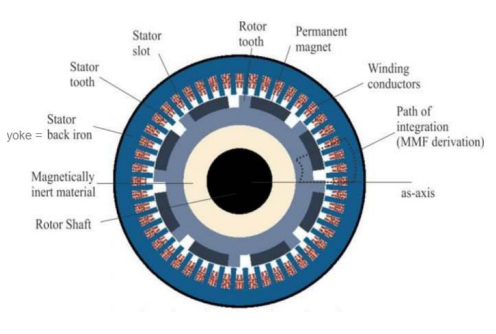
\includegraphics[width=0.6\textwidth]{assets/permanentemagneterotorinstator.png}
  \caption{Permanentemagneten rotor in stator}
  \label{fig:permanentemagneterotorinstator.png}
 \end{figure}
De rotor kan echter ook een \textbf{gladde rotor} zijn of een rotor met \textbf{uitspringende polen}, met een gladde rotor bedoelen we hier wel 'magnetisch glad' (weinig reluctantie), mechanisch heeft die gleuven met magneten. Uitspringende polen is vooral bij kleine machines en glad bij grote.
\newline
\newline
Hier zien we een figuur van permanente magneten en een rotor met DC-windingen, het veld word extern geëxciteerd met een veldstroom If:
\begin{figure}[H]
  \centering
  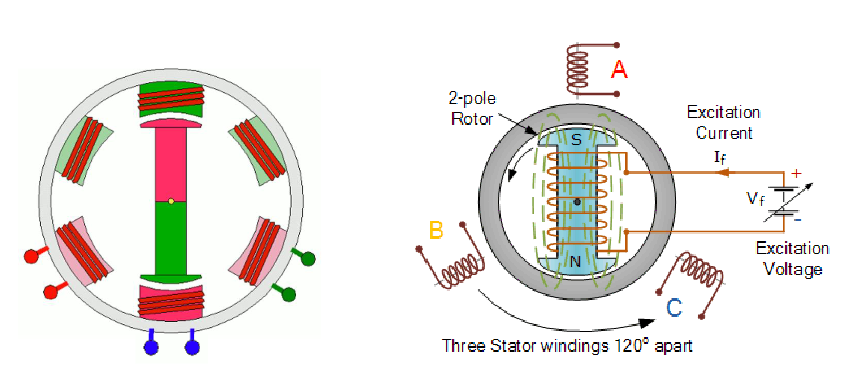
\includegraphics[width=0.6\textwidth]{assets/PMvsDCwindinge.png}
  \caption{PM vs DC windingen}
  \label{fig:PMvsDCwindinge.png}
 \end{figure}
\section{Stator en rotor magnetisch veld}
Eigelijk zijn er 2 draaivelden nu, we hebben dus het draaiveld van de stator dat opgewekt wordt door de 3AC dat we eerder bespraken maar we hebben ook een draaiveld in de rotor dat opgewekt wordt door de DC-windingen, maar let goed op, dit is een \textbf{constant} veld, het draait dus niet mee met de rotor. Het is dus de rotor die meegesleurd wordt door het draaiveld van de stator wat het dus doet lijken dat het veld van de rotor draait als je langs buiten kijkt of als je kijkt vanuit de stator zelf (want die staat stil).
\newline
\newline
Dus we hebben \textbf{$B_s$} dat het draaiveld van de stator is met elektrische pulsatie $\omega_s$ opgewekt door de 3AC en we hebben \textbf{$B_R$} dat het veld van de rotor is opgewekt door de DC-veldstroom $i_f$ in de rotor dat vast is tegenover de rotor maar mechanisch mee draait met de rotor. Deze 2 moeten dus dezelfde snelheid hebben want het statorveld sleurt de rotor mee, en hiermee wordt dus dat koppel gegenereerd met:
\begin{align*}
  \vv{T} = k \cdot \vv{B}_s \times \vv{B}_R
\end{align*}
k is trouwens een constante
\newline
\newline
Dan hebben we ook nog het \textbf{mutueel magnetisch veld} dat ontstaat door de interactie van de 2 velden, het is waar $B_s$ en $B_R$ samen komen en optellen tot één totaal veld:
\begin{align*}
  \vv{B}_{mut} = \vv{B}_s + \vv{B}_R
\end{align*}
De formule voor het koppel kan ook geschreven worden als:
\begin{align*}
  \vv{T} = k \cdot \vv{B}_{mut} \times \vv{B}_R
\end{align*}
Dit is exact hetzelfde als hierboven, als je dit uitwerkt kom je op dezelfde formule want dit werkt met kruisproducten, als je dit raar vind, vraag het aan AI.
\begin{figure}[H]
  \centering
  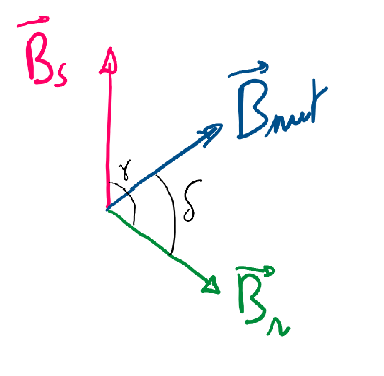
\includegraphics[width=0.4\textwidth]{assets/vectorschemaBsenBr.png}
  \caption{Vector schema van $B_s$ en $B_R$}
  \label{fig:vectorschemaBsenBr.png}
 \end{figure}
In de figuur hierboven zien we hoe $B_s$ en $B_R$ samen een mutueel veld vormen vectorieel weergegeven. Als je de vector formules van hierboven uitwerkt heb je per definitie altijd de hoek tussen je 2 vectoren nodig want $|\vv{A} \times \vv{B}| = |\vv{A}| \cdot |\vv{B}| \cdot \sin(\theta)$, en dit is dus de hoek tussen de 2 vectoren. De 2 hoeken voor deze vectoren zijn weergegeven op de figuur (met $\delta$ de koppelhoek, die we zometeen bespreken).
\begin{figure}[H]
  \centering
  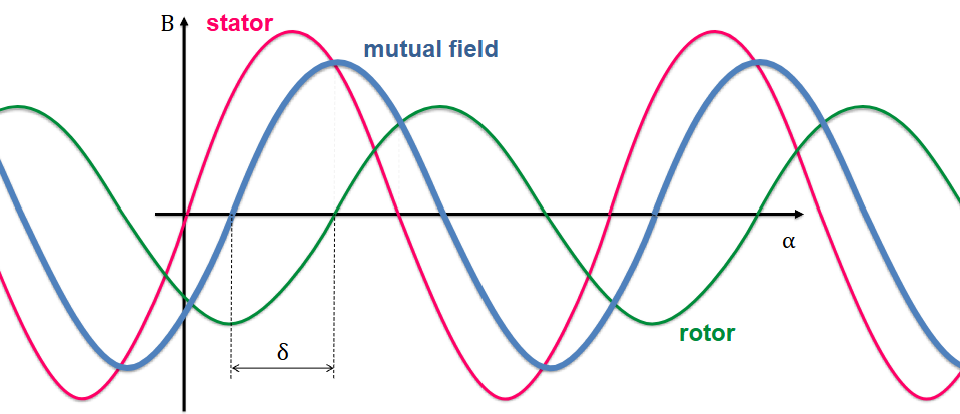
\includegraphics[width=0.5\textwidth]{assets/sinusoidaleweergavemutueelveld.png}
  \caption{Sinusoidale weergave van het mutueel veld}
  \label{fig:sinusoidaleweergavemutueelveld.png}
 \end{figure}
In de figuur hierboven zien we hoe het mutueel veld er uitziet in een sinusvorm, hier is de koppelhoek een faseverschuiving eigelijk. Dit is echter wel minder simpel weer te geven dan vectorieel dus vanaf nu doen we het gewoon vectorieel.
\section{Koppelhoek/Lasthoek}
De koppelhoek (ook wel lasthoek genoemd) is de hoek tussen het statorveld en het rotorveld, het wordt niet echt deftig vermeld op de slides of in de les maar in principe is het een elektrische hoek dat ook met het poolpaartal naar een mechanische hoek omgezet kan worden, echter werkt de proff in de slides met voorbeelden waar de machines 2 polen hebben en dus een poolpaartal van 1, daarom is het niet zo duidelijk want dan zijn die gewoon gelijk aan elkaar. Zoals we weten uit de vorige formules bepaalt deze hoek eigelijk het koppel dat de machine kan leveren met $T = k \cdot B_{mut} \cdot B_R \cdot \sin(\delta)$, op de volgende figuur zien we hoe het koppel wordt ontwikkeld voor elke toepassing van de synchrone machine:
\begin{figure}[H]
  \centering
  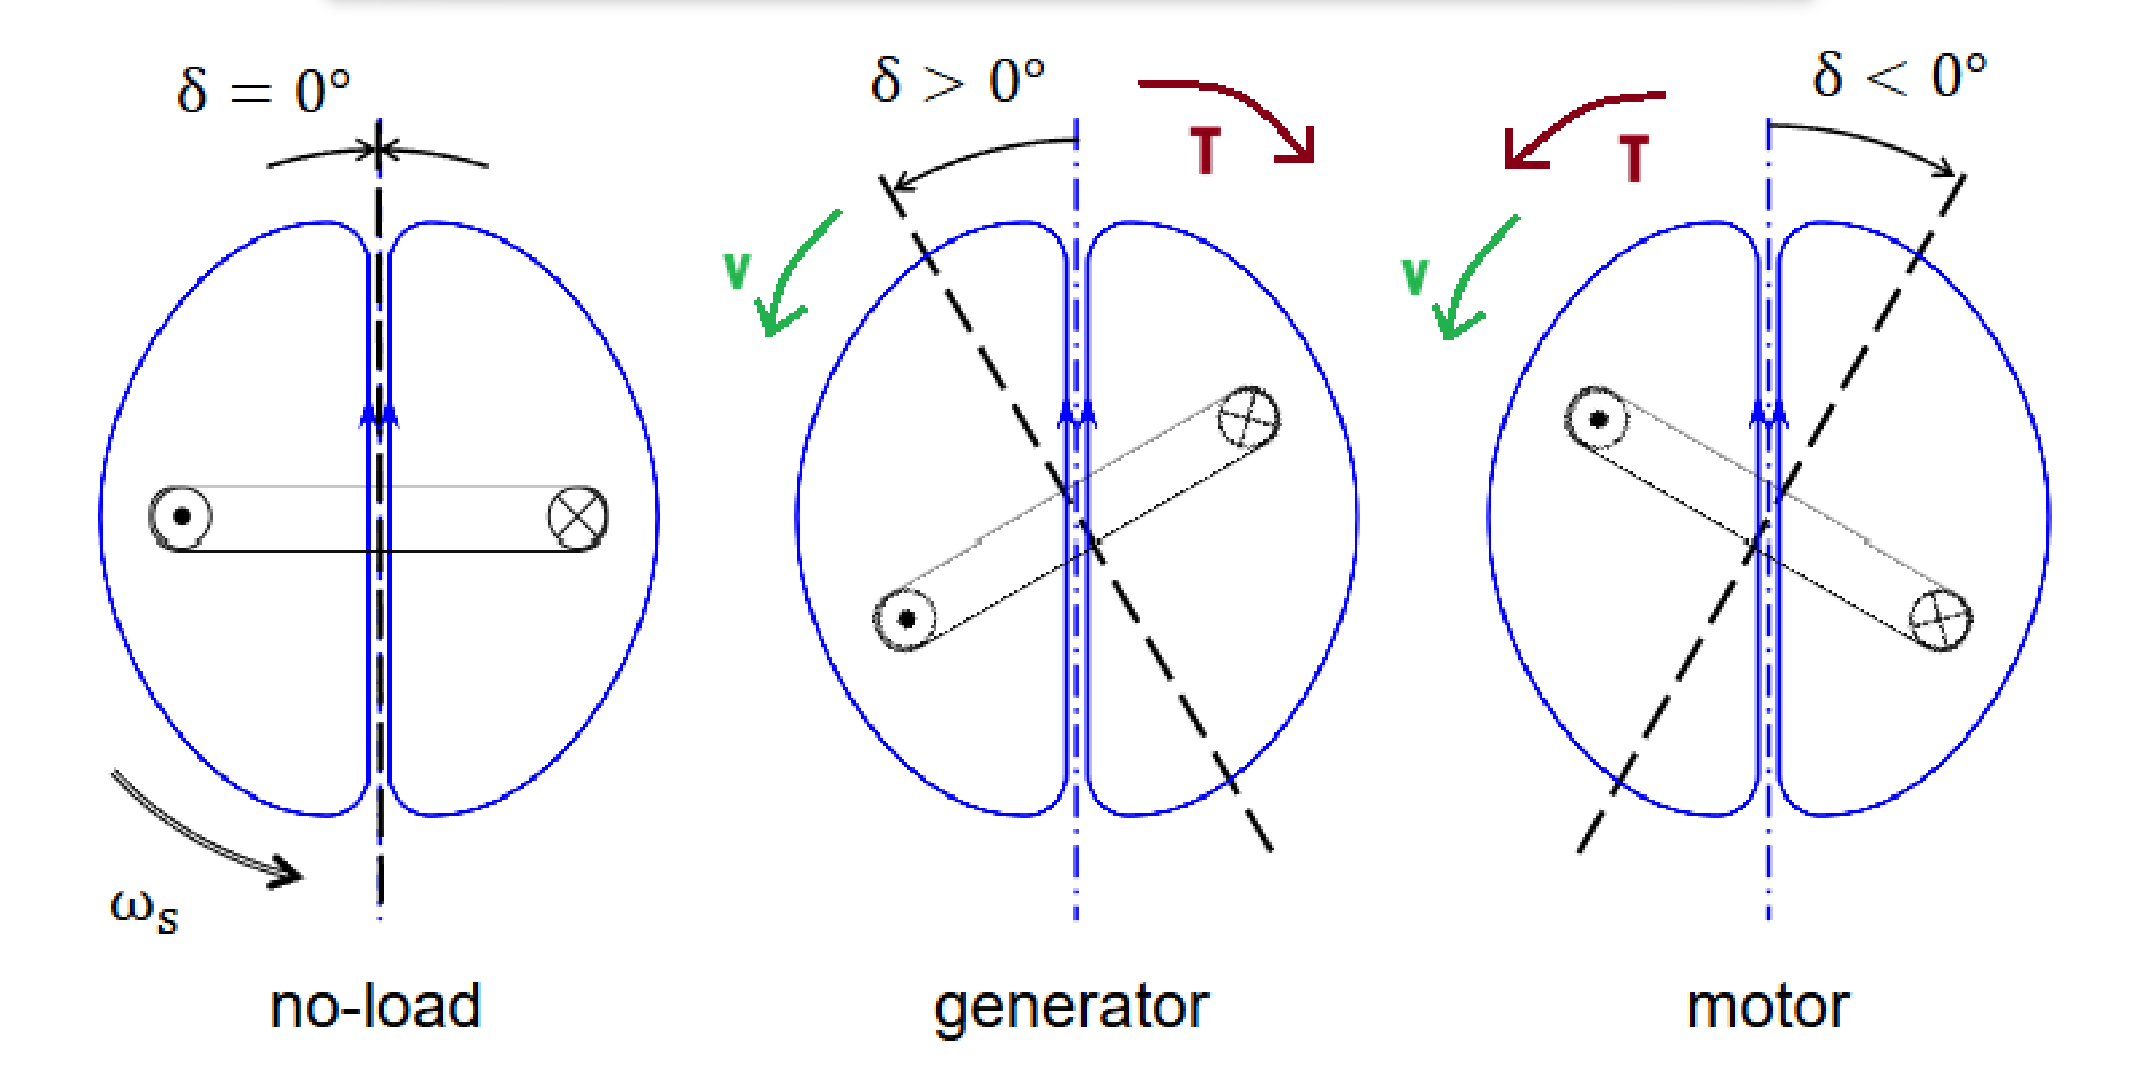
\includegraphics[width=0.6\textwidth]{assets/lasthoeknullastgeneratormotorsynchronemachine.png}
  \caption{Lasthoek bij nullast, generator en motor van een synchrone machine}
  \label{fig:lasthoeknullastgeneratormotorsynchronemachine.png}
 \end{figure}
\subsubsection{Nullast}
Dit is niet hetzelfde als stil staan, er is hier gewoon geen last (dus \textbf{geen koppel, $T = 0$}). De \textbf{motor draait wel op volle snelheid} daardoor en de stator trekt de rotor dus niet mee, er is dus een \textbf{koppelhoek van 0°}.
\subsubsection{Generator}
Hier ijlt de rotor voor op het mutueel veld, hierdoor wordt er een koppel ontwikkeld dat de rotor tegenhoudt, eigelijk tegenin de beweging van de rotor in, \textbf{de rotor trekt dus het magnetisch veld mee}, het \textbf{koppel is tegengesteld aan de lasthoek} want het wilt het terug brengen naar 0°. Een referentie die we nemen om te zeggen of de hoekpositie van de lasthoek positief is, is als hij in dezelfde richting is als de draaizin, wat hier het geval is, dus de \textbf{lasthoek is positief.}
\subsubsection{Motor}
Hier wordt de rotor meegetrokken door het mutueel veld, dit wordt dus gecreëerd door de 3AC die het draaiveld vormen. Het koppel werkt mee met de snelheid, doordat de rotor achterloopt is de \textbf{lasthoek} in de andere richting als de beweging en dus \textbf{negatief}. Hoe groter deze hoek tho (negatiever dan), hoe groter het koppel.

\section{Berekening van de geïnduceerde spanning}
We hebben dus onze 3AC machine met een stilstaande stator en een rotor die een constant veld heeft en in de stator draait, dat constant veld dat door een DC-winding wordt opgewekt gaat eigelijk langs de stator windingen passeren omdat de rotor draait en dus daardoor een spanning induceren in de stator wikkelingen, deze gaan we nu berekenen hoe groot die is.
\begin{figure}[H]
  \centering
  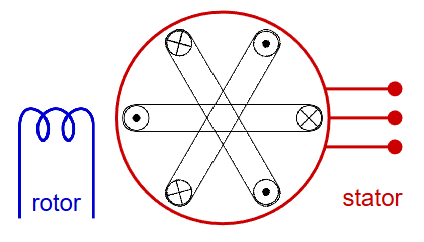
\includegraphics[width=0.6\textwidth]{assets/rotor_stator_doorsnede.png}
  \caption{Doorsnede van rotor en stator: de statorwikkeling bestaat uit 3 fasen, elk met hun eigen vaste positie $\theta$ rond de omtrek.}
  \label{fig:rotor_stator_doorsnede}
\end{figure}

\subsubsection{Flux gezien door een statorspoel}
Elke statorspoel zit op een \textit{vaste positie} $\theta_x$. De mutuele flux die spoel $a$ (op positie $\theta_a$) ziet, is:
\begin{align*}
    \Phi_{mut,a} = \hat{\Phi} \cdot \cos(\omega_s t - p\theta_a)
\end{align*}
Omdat de drie fasespoelen elk op een andere positie ($\theta_a$, $\theta_b$, $\theta_c$, telkens 120° elektrisch uit elkaar) rond de omtrek zitten, zien ze alle drie een \textbf{andere} flux, vandaar dat elke fase zijn eigen (in tijd verschoven) spanning krijgt.

\subsubsection{Geïnduceerde spanning via Faraday}
Met de wet van Faraday, $e = -N\dfrac{d\Phi}{dt}$, en $\Phi_a(t) = \hat{\Phi}\cos(\omega_s t)$ voor spoel $a$ (referentiepositie $\theta_a=0$):
\begin{align*}
    e_a(t) = -N\frac{d\Phi_a}{dt} = N\hat{\Phi}\,\omega_s \sin(\omega_s t)
\end{align*}
Met de piekwaarde $\hat{E} = N\hat{\Phi}\,\omega_s$ (op tekenconventie na, afhankelijk van de gekozen positieve richting) geeft dit voor de drie fasen:
\begin{align*}
    e_a(t) &= -\hat{E}\cdot\sin(\omega_s t) \\
    e_b(t) &= -\hat{E}\cdot\sin(\omega_s t - 120^\circ) \\
    e_c(t) &= -\hat{E}\cdot\sin(\omega_s t - 240^\circ)
\end{align*}

\subsubsection{Effectieve waarde}
De effectieve (RMS) waarde volgt weer uit de piekwaarde gedeeld door $\sqrt{2}$:
\begin{align*}
    \boxed{E = \sqrt{2}\pi N_c \hat{\Phi} f = k\hat{\Phi}\omega}
\end{align*}
Dit komt exact overeen met de formule uit de vorige sectie. Merk ook op dat $E \sim I_f$ (evenredig met de rotor-veldstroom), net zoals bij de magnetisatiecurve die we eerder zagen, maar geld dus ook niet heel de tijd.

\subsubsection{Aansluiting van de statorwikkeling}
De drie fasewikkelingen van de stator kunnen op twee manieren met elkaar verbonden worden: in \textbf{ster (Y)} of in \textbf{driehoek ($\Delta$)}. Deze keuze bepaalt de verhouding tussen lijn- en fasespanning/-stroom, en komt later uitgebreider aan bod.

\subsubsection{Faseverhouding tussen flux, spanning en stroom}
\begin{figure}[H]
  \centering
  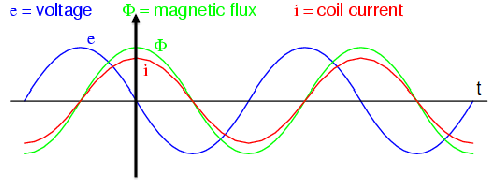
\includegraphics[width=0.7\textwidth]{assets/golfvormen_flux_spanning_stroom.png}
  \caption{Tijdsverloop van flux $\Phi$, geïnduceerde spanning $e$ en stroom $i$ in één fase.}
  \label{fig:golfvormen_flux_spanning_stroom}
\end{figure}

Uit de grafiek volgt de logische volgorde: de flux $\Phi$ (cosinusvorm) bereikt zijn piek op $t=0$; de spanning $e=-N\,d\Phi/dt$ loopt daar $90^\circ$ op achter (nul op $t=0$, want de afgeleide van een piek is nul); En die stroom i \textbf{is het model van de rotorstroom, het is de stroom die die groene flux \textit{zou} maken als je het in de stator zou laten lopen, het is gewoon wat het zelfde effect zou geven. {\color{red}Dit is dus geen echte stroom!}}
\subsection{Magnetisatiecurve}
Dit hebben we eerder al wat gezien, maar komt terug rap voor op de slides. Een andere benaming hier voor is trouwens de \textit{nullastkarakteristiek} of \textit{open circuit karakteristiek}.
\begin{figure}[H]
  \centering
  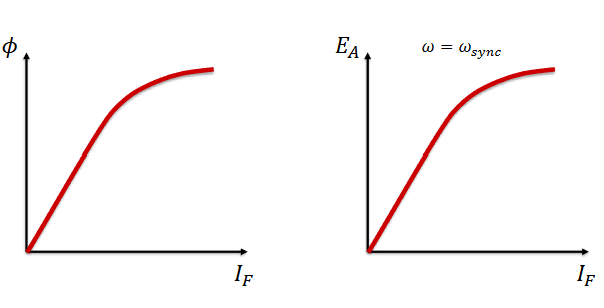
\includegraphics[width=0.6\textwidth]{assets/magnetscurves.png}
  \caption{Magnetisatiecurven}
  \label{fig:magnetscurves.png}
 \end{figure}
Bij de linkse curves zien we dat er even een lineair verband is tussen de hoeveelheid flux en de veldstroom, maar dat dit na een bepaalde waarde niet meer zo is (saturatie) en dat het veld maar een klein beetje meer toeneemt bij veel meer veldstroom. De rechtse curve meten we door de spanning te meten bij een open klem (nullast) en op constante volle snelheid van de motor (want $E = k\Phi\omega$).
\newline
\newline
Een belangrijk ding om op te merken is wel dat de inwendige spanning eigelijk toch niet helemaal hetzelfde is als de klemspanning, dit komt door volgende verschillende effecten:
\begin{itemize}
   \item \textbf{Ankerreactie}: Dit is de belangrijkste, deze bespreken we zometeen uitgebreid
   \item \textbf{Zelfinductantie anker}: Dit is niet echt uitgelegd maar dit is gewoon de zelfinductantie van de statorwikkelingen, dit is een beetje zoals bij een DC-machine, als je een stroom door een spoel stuurt dan zal er een tegen EMK ontstaan dat de stroom tegenwerkt. Dit is dus ook zo bij de statorwikkelingen, als er een stroom doorheen gaat dan zal er een tegen EMK ontstaan dat de stroom tegenwerkt.
   \item \textbf{Ankerweerstand}: De weerstand van de statorwikkelingen
   \item \textbf{Uitspringende polen}: Dit is een mechanisch effect, dit is wel 'extra' dus is eigelijk niet belangrijk
\end{itemize}
\section{Ankerreactie}
Ankerreactie is simpelweg de stroom in de stator dat ook een veld veroorzaakt dat het totale veld verstoort. Hiervoor kijken we naar de fasediagrammen:
\begin{figure}[H]
  \centering
  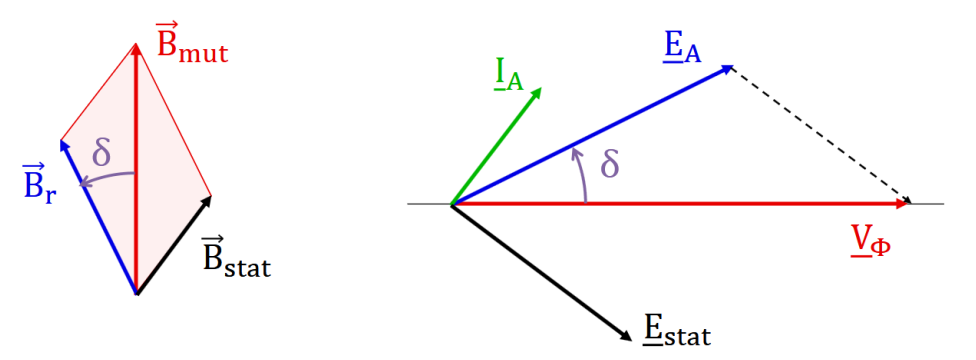
\includegraphics[width=0.6\textwidth]{assets/fasediagrammen.png}
  \caption{Fasediagram veld en Stroom/spanningen synchrone motor (Deze figuur is voor de Onderbekrachtigde Generator)}
  \label{fig:fasediagrammen.png}
 \end{figure}
We hebben dus het veld van de rotor $\vv{B}_R$ dat onder een bepaalde geometrische hoek in de ruimte staat, het is dit veld dat de inwendige spanning $\underline{E}_A$ induceert in de statorwikkelingen. Als we dan onze motor gaan belasten dan zal er dus ook een stroom gaan lopen in de statorwikkelingen, dit is de stroom $\underline{I}_A$, het is deze stroom dat dan ook een magnetisch veld induceerd in de stator, dit is die ankerreactie eigelijk, het is $\vv{B}_{Stat}$ dat samen met $\vv{B}_R$ een mutueel veld vormt $\vv{B}_{mut}$ dat de rotor dus mee trekt. Het veld van de stator $\vv{B}_{Stat}$ induceert dan ook nog $\underline{E}_{Stat}$ (de spanningsval over de statorreactantie), deze bepaald eigelijk of de klemspanning $\underline{V}_{\phi}$ groter of kleiner is dan de inwendige spanning $\underline{E}_A$.
\begin{warningbox}[Koppelhoek in deze figuur verschilt!]
    Let op want in de linkse figuur is de \textit{koppelhoek} bij die velden daar een \textbf{geometrische} hoek, maar in de rechtse figuur is dit de \textit{lasthoek}, dit is in het \textit{frequentiedomein} (tijd), het is een weergave voor \textbf{elektrische} grootheden dus!
\end{warningbox}
We kunnen de klemspanning dan ook als volgt schrijven:
\begin{align*}
    \underline{V}_{\phi} = \underline{E}_A + \underline{E}_{Stat}
\end{align*}
Hierbij is $\underline{E}_{Stat} = -j \cdot X \cdot \underline{I}_A$, dus de ankerreactie wat te wijten is aan het feit dat de statorstroom het veld eigelijk verstoord. Het is negatief omdat de stroom hier \textit{voor} ijlt op de spanning.
\newline
\newline
We hebben echter ook wel nog een zelfinductantie en een ankerweerstand, dus de volledige vergelijking wordt dan:
\begin{equation*}
\underline{V}_{\phi} = \underline{E}_A
- \underbrace{\textcolor{blue}{j \cdot X \cdot \underline{I}_A}}_{\textcolor{blue}{\text{ankerreactie}}}
- \underbrace{\textcolor{red}{j \cdot X_A \cdot \underline{I}_A}}_{\textcolor{red}{\text{zelfinductantie}}}
- \underbrace{\textcolor{teal}{\underline{I}_A \cdot R}}_{\textcolor{teal}{\text{ankerweerstand}}}
\end{equation*}
Hierbij is die zelfinductantie eigelijk de invloed van \textbf{de stator OP DE STATOR} zonder dat zelfs die rotor invloed heeft, het is gewoon lekflux eigelijk. $X_A$ is de impedantie van de ankerreactie terwijl X de zelfinductantie is van het anker, we gaan deze 2 samen nemen als $X_S$ zodat we het volgende krijgen:
\begin{align*}
    \underline{V}_{\phi} = \underline{E}_A - j \cdot X_S \cdot \underline{I}_A - \underline{I}_A \cdot R
\end{align*}
In ons equivalent model gaan we de ankerweerstand wel verwaarlozen, we gaan dus idealiseren. Dit maakt het dat we geen rendement kunnen bepalen, op het examen verwaarlozen we dit ook maar kan ze het wel als theorievraag vragen wat het effect daarvan is. We hebben dus:
\begin{align*}
    \underline{V}_{\phi} = \underline{E}_A - j \cdot X_S \cdot \underline{I}_A \\
    \rightarrow \underline{V}_{\phi} = j \cdot X_r \cdot \underline{I}_r - j \cdot X_S \cdot \underline{I}_A
\end{align*}
Hierboven is $E_A$ uitgeschreven als het model van het magnetisch effect van de rotor op de stator met die rotorstroom $I_r$ dat eigelijk niet bestaat en de AC stroom zou zijn dat het zelfde veld opwekt.
\newpage
\section{Equivalent schema}
In de volgende figuur zien we het equivalent circuit/model met een generatorreferentie:
\begin{figure}[H]
  \centering
  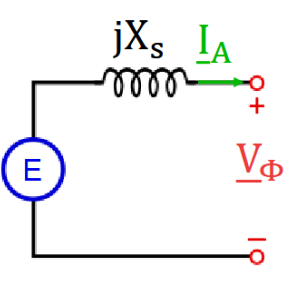
\includegraphics[width=0.3\textwidth]{assets/equivgenerref.png}
  \caption{Equivalent schema van een synchrone machine met generatorreferentie}
  \label{fig:equivgenerref.png}
 \end{figure}
De volgende figuur is dit dan voor een motorreferentie:
\begin{figure}[H]
  \centering
  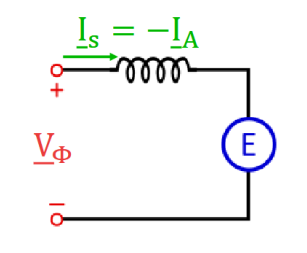
\includegraphics[width=0.3\textwidth]{assets/equimotorref.png}
  \caption{Equivalent schema van een synchrone machine met motorreferentie}
  \label{fig:equimotorref.png}
 \end{figure}
\subsection{Soorten metingen}
Er zijn een aantal proeven die we kunnen doen om de parameters te bepalen uit de formule die we zojuist zagen, het gaat hier dan vooral om $E_A$ en $X_S$.
\subsubsection{Nullastproef}
Hierbij gaan we de rotor aandrijven tot de nominale (synchrone) snelheid en het veld bekrachtigen met een aparte DC-bron en een regelbare weerstand die $I_f$ regelt. De statorklemmen laten we open zodat $I_A = 0$ en dus de formule herleid naar:
\begin{align*}
    \underline{V}_{\phi} = \underline{E}_A
\end{align*}
De klemspanning kunnen we meten dus we hebben dan $E_A$ voor die specifieke $I_f$, dit doen we voor verschillende veldstromen (stap verhogen steeds) om zo de volgende O.C.C. kromme op te bouwen (O.C.C. = Open Circuit Characteristic):
\begin{figure}[H]
  \centering
  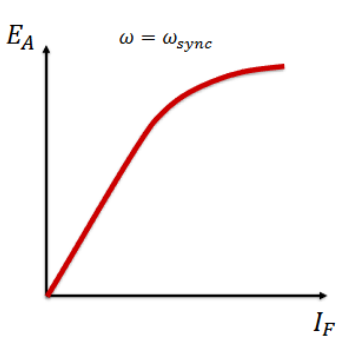
\includegraphics[width=0.3\textwidth]{assets/OCCcurve.png}
  \caption{O.C.C.}
  \label{fig:OCCcurve.png}
 \end{figure}
\begin{warningbox}[Hysteresis]
    Bij het verhogen van die stappen mag je NOOIT verlagen (terugdraaien) want je hebt hier hysteresis, ook zie je op het einde van de curve dat deze afbuigt, dit is verzadiging.
\end{warningbox}
\subsubsection{Kortsluitproef}
Dit heeft dezelfde opstelling, rotor tot nominale snelheid en veld bekrachtigen met aparte DC bron maar nu gaan we de statorklemmen kortsluiten zodat $V_{\phi} = 0$ en dus de formule herleid naar:
\begin{align*}
    0 = \underline{E}_A - j \cdot X_S \cdot \underline{I}_A \\
    \rightarrow j \cdot X_S \cdot \underline{I}_A = \underline{E}_A
\end{align*}
Zo meet je eigelijk $I_A$ ( = $I_{SC}$) voor verschillende veldstromen. En omdat de kortsluitstroom via ankerreactie het netveld sterk demagnetiseert, blijft de curve hier in het lineaire (onverzadigde) gebied, hoe groot $I_f$ ook is.
\begin{figure}[H]
  \centering
  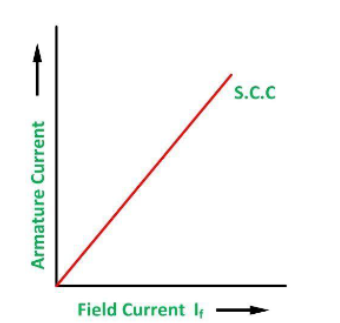
\includegraphics[width=0.3\textwidth]{assets/SCCcurve.png}
  \caption{S.C.C.}
  \label{fig:SCCcurve.png}
 \end{figure}
\subsubsection{Bepaling van de parameters}
Kies nu een veldstroom $I_f$ in de O.C.C. en lees de corresponderende $E_A$ af. Kies dezelfde $I_f$ in de S.C.C. en lees de corresponderende $I_{SC}$ af. Zo kan je dan $X_S$ berekenen met:
\begin{align*}
    X_S = \frac{E_A}{I_{SC}}
\end{align*}
\section{Fasediagrammen}
Via het equivalent circuit gaan we dus ook fasediagrammen kunnen opstellen, dit zijn grafische weergaven van de grootheden in het complex vlak. We hebben voor de synchrone machine een motorreferentie en een generatorreferentie, deze verschillen dus. Ook kunnen ze verschillen in over en onderbekrachtiging, dit is afhankelijk van de veldstroom $I_f$ en de statorstroom $I_A$. In de volgende figuren zien we de fasediagrammen voor een generator en een motor, beide onder en overbekrachtigd:
\begin{figure}[H]
  \centering
  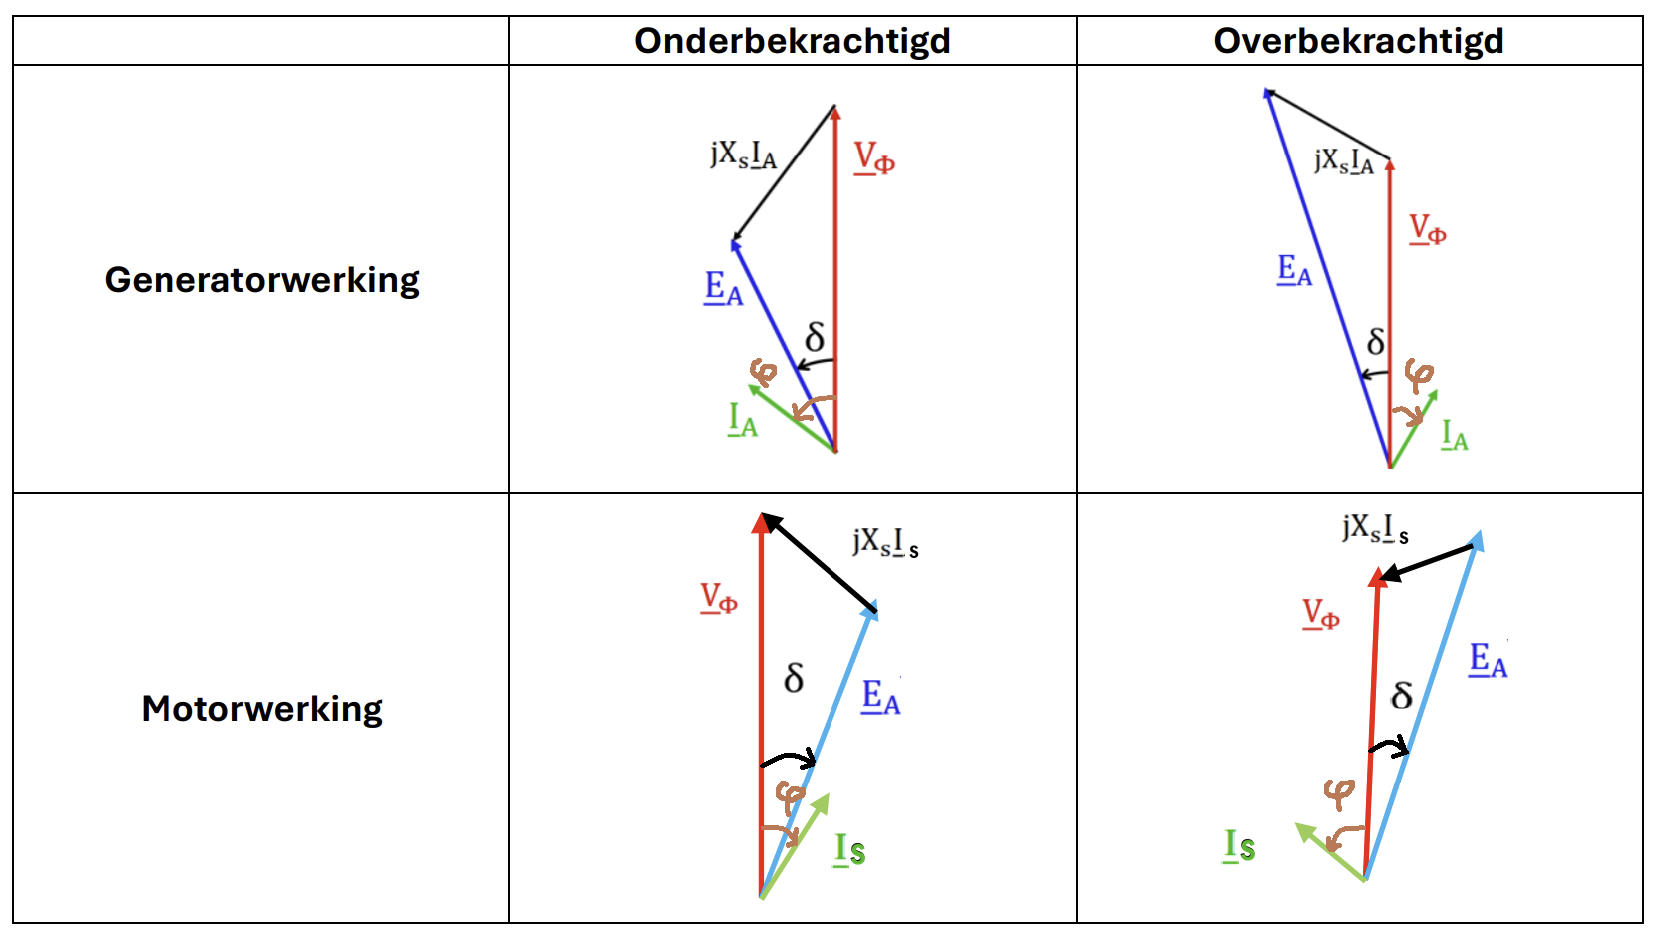
\includegraphics[width=0.8\textwidth]{assets/fasediragmamee.png}
  \caption{Fasediagrammen motor en generator, onder en overbekrachtigd}
  \label{fig:fasediragmamee.png}
 \end{figure}
Wat wel belangrijk is om op te merken is dat bij motorwerking we niet meer met $I_A$ werken maar met $I_S$ (de statorstroom, want de machine neemt nu stroom op), en wat nog belangrijker is, is dat deze het \textbf{tegenovergestelde} is van $I_A$ dus $I_A = - I_S$! En dus voor de motor geldt:
\begin{align*}
    \underline{V}_{\phi} = \underline{E}_A + j \cdot X_S \cdot \underline{I}_S
\end{align*}
\subsection{Onderbekrachtiging}
Bij onderbekrachtiging is het rotorveld ($I_f$) te zwak, hierdoor is er te weinig flux in de machine en gaat de stator dit moeten compenseren door een hogere stroom te trekken, dit zorgt voor meer veld ($\vv{B}_{Stat}$) want als de flux daalt, daalt de inwendige spanning $E_A$ en stijgt dus de statorstroom $I_S$. Bij een motor wordt dit dus inductiever en bij een generator capacitiever. Onderbekrachtigd zorgt dus dat de koppelhoek groter wordt, het kan de rotor meesleuren maar het loopt meer achter.
\subsection{Overbekrachtiging}
Bij overbekrachtiging is het rotorveld ($I_f$) te sterk, hierdoor is er te veel flux in de machine en gaat de stator dit moeten tegenwerken door een lagere stroom te trekken, de stator voert dus eigelijk magnetisch veld af (levert dus reactief vermogen) wat het bij de motor capacitiever maakt en bij de generator inductiever. De stator wilt de rotor eigelijk afremmen waardoor de koppelhoek kleiner wordt.
\section{Vermogen en koppel}
Voor het bepalen van het vermogen van de synchrone machine gaan we van uit van een ideale machine waarbij dus geldt dat het elektrisch vermogen gelijk is aan het mechanisch vermogen, dus een rendement van 100. Ook gaan we uit van een star net, dus een constante fasespanning:
\begin{align*}
    P_{elektrisch} = P_{mechanisch}
\end{align*}
Het elektrisch vermogen kunnen we schrijven als:
\begin{align*}
    \sqrt{3} \cdot U_L \cdot I_L \cdot \cos(\varphi) = 3 \cdot \underbrace{V_{\phi}}_{\text{Constant!}} \cdot I_A \cdot \cos(\varphi)
\end{align*}
Met het fasordiagram (simpele geometrie dat het stukje $I_A \cdot \cos(\varphi)$ verandert door $\frac{\sin(\delta) \cdot E_A}{X_S}$) kunnen we dit ook schrijven als:
\begin{align*}
    P_{elektrisch} = P_{mechanisch} = P = 3 \cdot \frac{V_{\phi} \cdot E_A}{X_S} \cdot \sin(\delta)
\end{align*}
Dit is dus de formule voor het vermogen bij een ideale machine, dit is een sinusvormige functie. Het koppel kan dus ook bepaald worden met de formule $P = T \cdot \omega$.
\subsection{Synchronisatieverliezen}
Dat sinusvormige vermogen is dus afhankelijk van de koppelhoek $\delta$ en is maximaal op $\delta = 90^\circ$, hierna daalt dit vermogen terug. We willen dus eigelijk rond die 90 graden werken maar we doen het in de praktijk niet door synchronisatieverliezen. Bij synchronisatieverlies gaan we over de maximale koppel gaan, waardoor we niet genoeg vermogen meer gaan hebben waardoor we eigenlijk niet meer synchroon gaan draaien, we lopen eigelijk achter en onze hoek wordt dus groter, dit kan zo uitlopen tot we uiteindelijk een volledige toer achter zitten. Toeren kunnen we terugwinnen door de snelheid op te trekken, er is dus acceleratie nodig. Daarom werken we rond een gebied van $20^\circ-30^\circ$.
\begin{figure}[H]
  \centering
  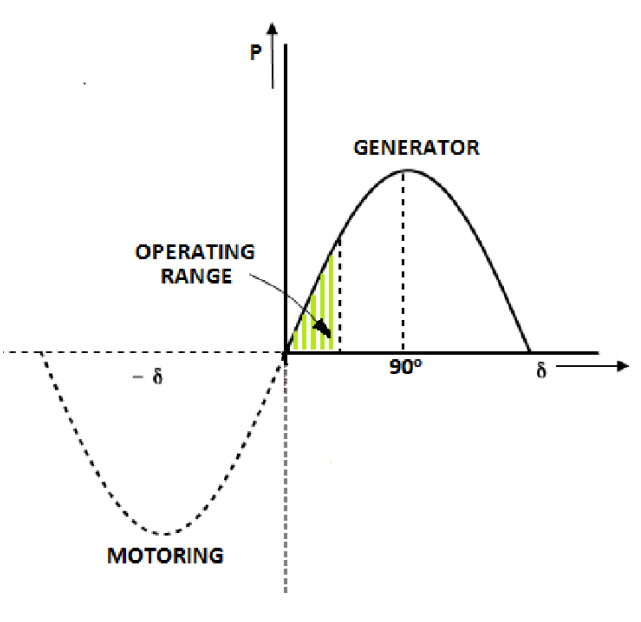
\includegraphics[width=0.5\textwidth]{assets/werkingsgebiedvoorsynchronisatieverliesµ.png}
  \caption{Vermogen ifv koppelhoek, met aanduiding van het werkingsgebied voor synchronisatieverlies}
  \label{fig:werkingsgebiedvoorsynchronisatieverliesµ.png}
 \end{figure}
Een plotse verandering van last (lasthoek wordt even heel groot want de rotor vertraagt even) kan wel zorgen voor een transiënte snelheid verandering, deze gaat uiteindelijk wel naar zijn oorspronglijke synchrone snelheid (steady-state). Maar een te grote verandering van last kan dus toeren doen missen of de motor doen stilvallen.
\begin{figure}[H]
  \centering
  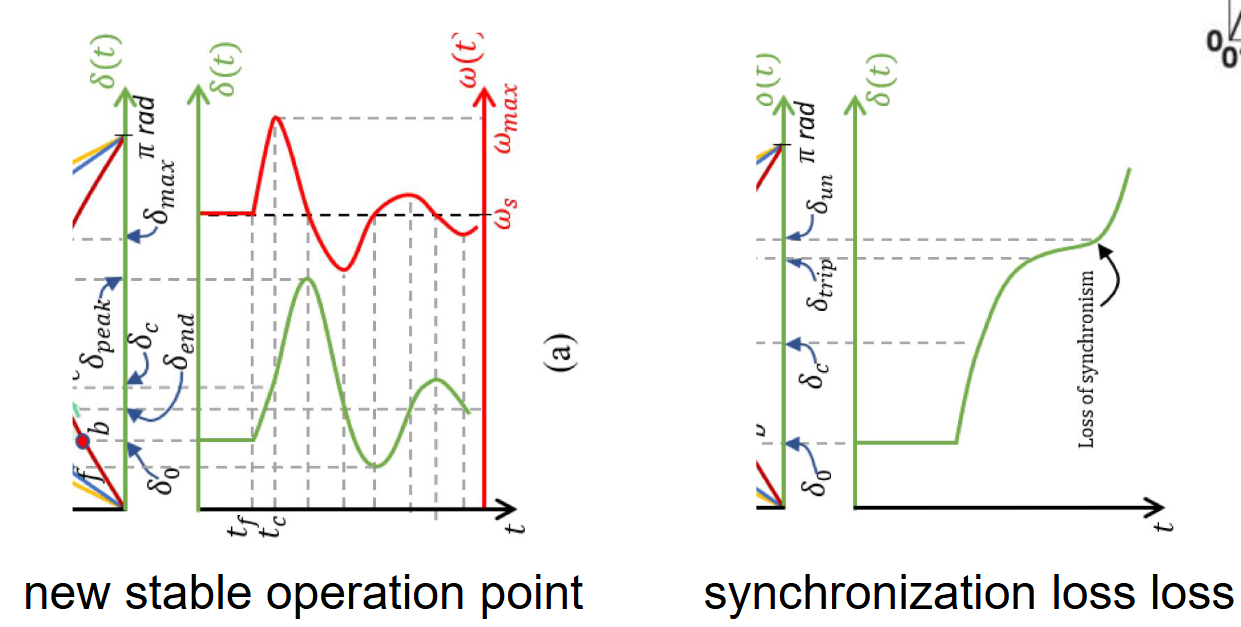
\includegraphics[width=0.6\textwidth]{assets/transienteensynchronisatieverlies.png}
  \caption{Linkse plot terug naar stabiele toestand, rechtse plot naar synchronisatieverlies}
  \label{fig:transienteensynchronisatieverlies.png}
 \end{figure}
\subsection{Verschil in rotorconstructie}
Als je bij een glade rotor geen stroom hebt in de rotor maar wel in stator dan gaat je draaiveld geen invloed hebben op de rotor, er is dus geen koppel. Bij een rotor met polen ga je wel een koppel hebben, dit is omdat het ijzer van die polen eigelijk wilt alligneren met dat magnetisch draaiveld, ze nemen het pad van minste \textbf{reluctantie}. Dit noemt dus een reluctantiekoppel en heeft dus een reluctantievermogen. Dit draagt bij aan het totaal vermogen:
\begin{figure}[H]
  \centering
  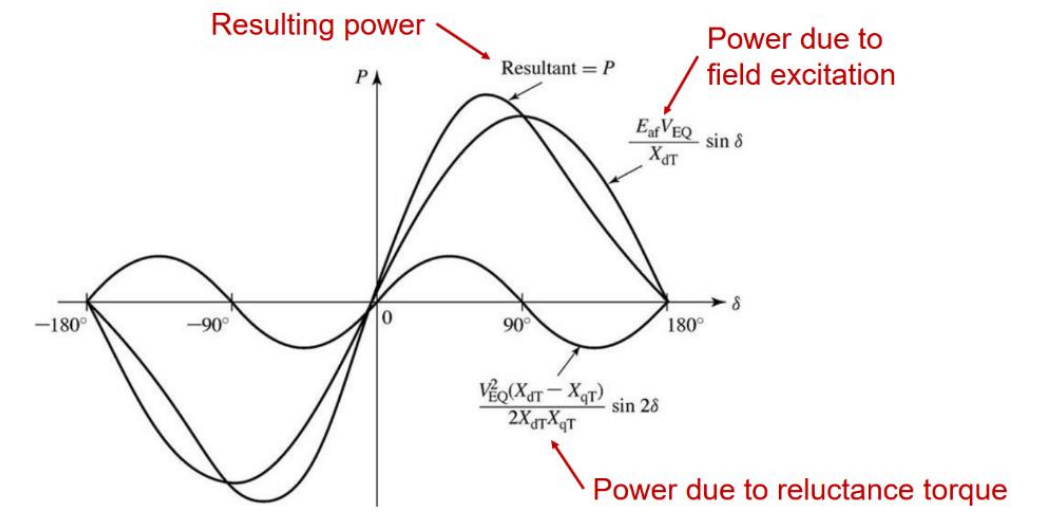
\includegraphics[width=0.6\textwidth]{assets/invloedrelucatnievermoge.png}
  \caption{Invloed reluctantievermogen}
  \label{fig:invloedrelucatnievermoge.png}
 \end{figure}
Dit reluctantievermogen piekt op een hoek van $45^\circ$ en is dus veroorzaakt door de vorm van de rotor.
\section{Synchrone Generator}
\subsection{Eilandbedrijf}
Een synchrone generator kan in eilandbedrijf werken, dit wil zeggen dat hij niet verbonden is met een groot net maar dat hij zelf een net vormt. (Stand-alone). Bvb een windturbine die een huis van stroom voorziet (lijkt mij straf ma dit is een voorbeeld). We gaan nu eens kijken wat er gebeurt als de belasting hierop varieert, want deze doet de grootte van $I_A$ veranderen.
\begin{figure}[H]
  \centering
  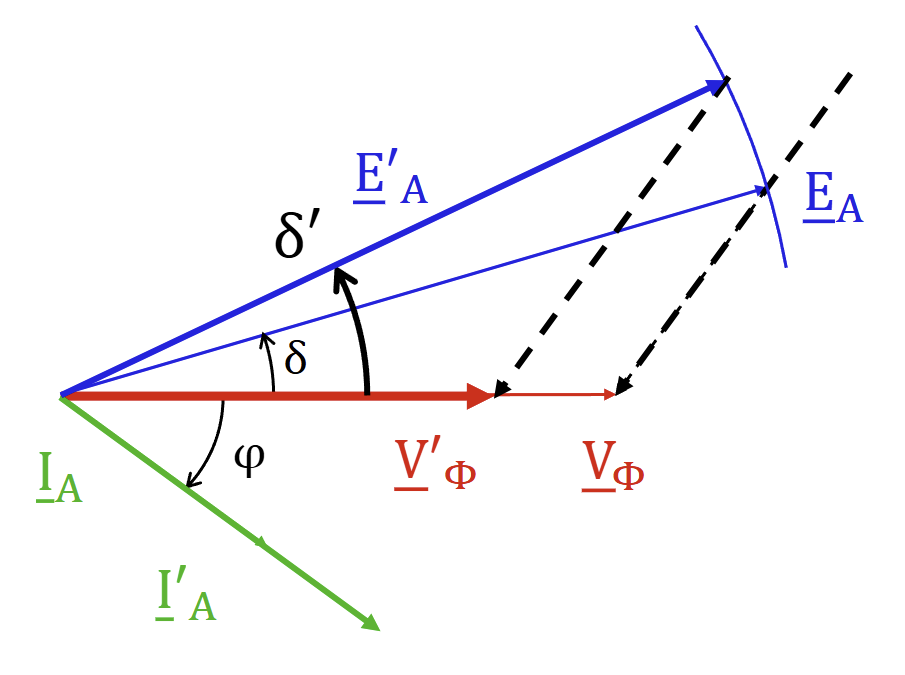
\includegraphics[width=0.5\textwidth]{assets/varierendebelastinggeneratoreilandbedrijf.png}
  \caption{Fasediagrammen bij variërende belasting van een synchrone generator in eilandbedrijf}
  \label{fig:varierendebelastinggeneratoreilandbedrijf.png}
 \end{figure}
We weten dat meer belasting zorgt voor een grotere lasthoek, en aangezien $E_A$ afhankelijk is van de bekrachtiging $I_f$ blijft deze constant, je ziet dat daardoor $V_{\phi}$ kleiner is geworden en de stroom groter. Als we $V_{\phi}$ groter willen zullen we met de bekrachtiging moeten spelen om $E_A$ groter te maken.
\subsection{Meerdere (Parallelle) generatoren}
Je kan ook meerdere generatoren in parallel zetten, dit heeft als voordelen dat dit meer betrouwbaar is want als één uitvalt werkt de rest wel nog, veel generatoren zorgen ook voor een stabieler net. Condities die nodig zijn voor het parallel schakelen zijn de volgende:
\begin{itemize}
    \item Ze moeten dezelfde spanning hebben
    \item Ze moeten dezelfde frequentie hebben
    \item Ze moeten dezelfde fasehoek hebben
    \item Ze moeten dezelfde fasevolgorde (fase sequentie) hebben
\end{itemize}
Ze moeten niet percee de zelfde snelheid of zelfde poolpaartal hebben (behalve als ze op de zelfde as zitten)
\begin{conceptbox}[Star net]
    Een star net is een net waarvan de spanning constant is, hier zijn een groot aantal generatoren parallel geschakeld. Ze hebben een systeem operator (zoals Elia)
\end{conceptbox}
\subsection{Rating van een synchrone generator}
Nu gaan we kijken naar de limieten van de synchrone machine, dit is belangrijk want we willen weten wat de maximale belasting is die we kunnen leveren. We hebben hiervoor een aantal limieten.
\begin{figure}[H]
  \centering
  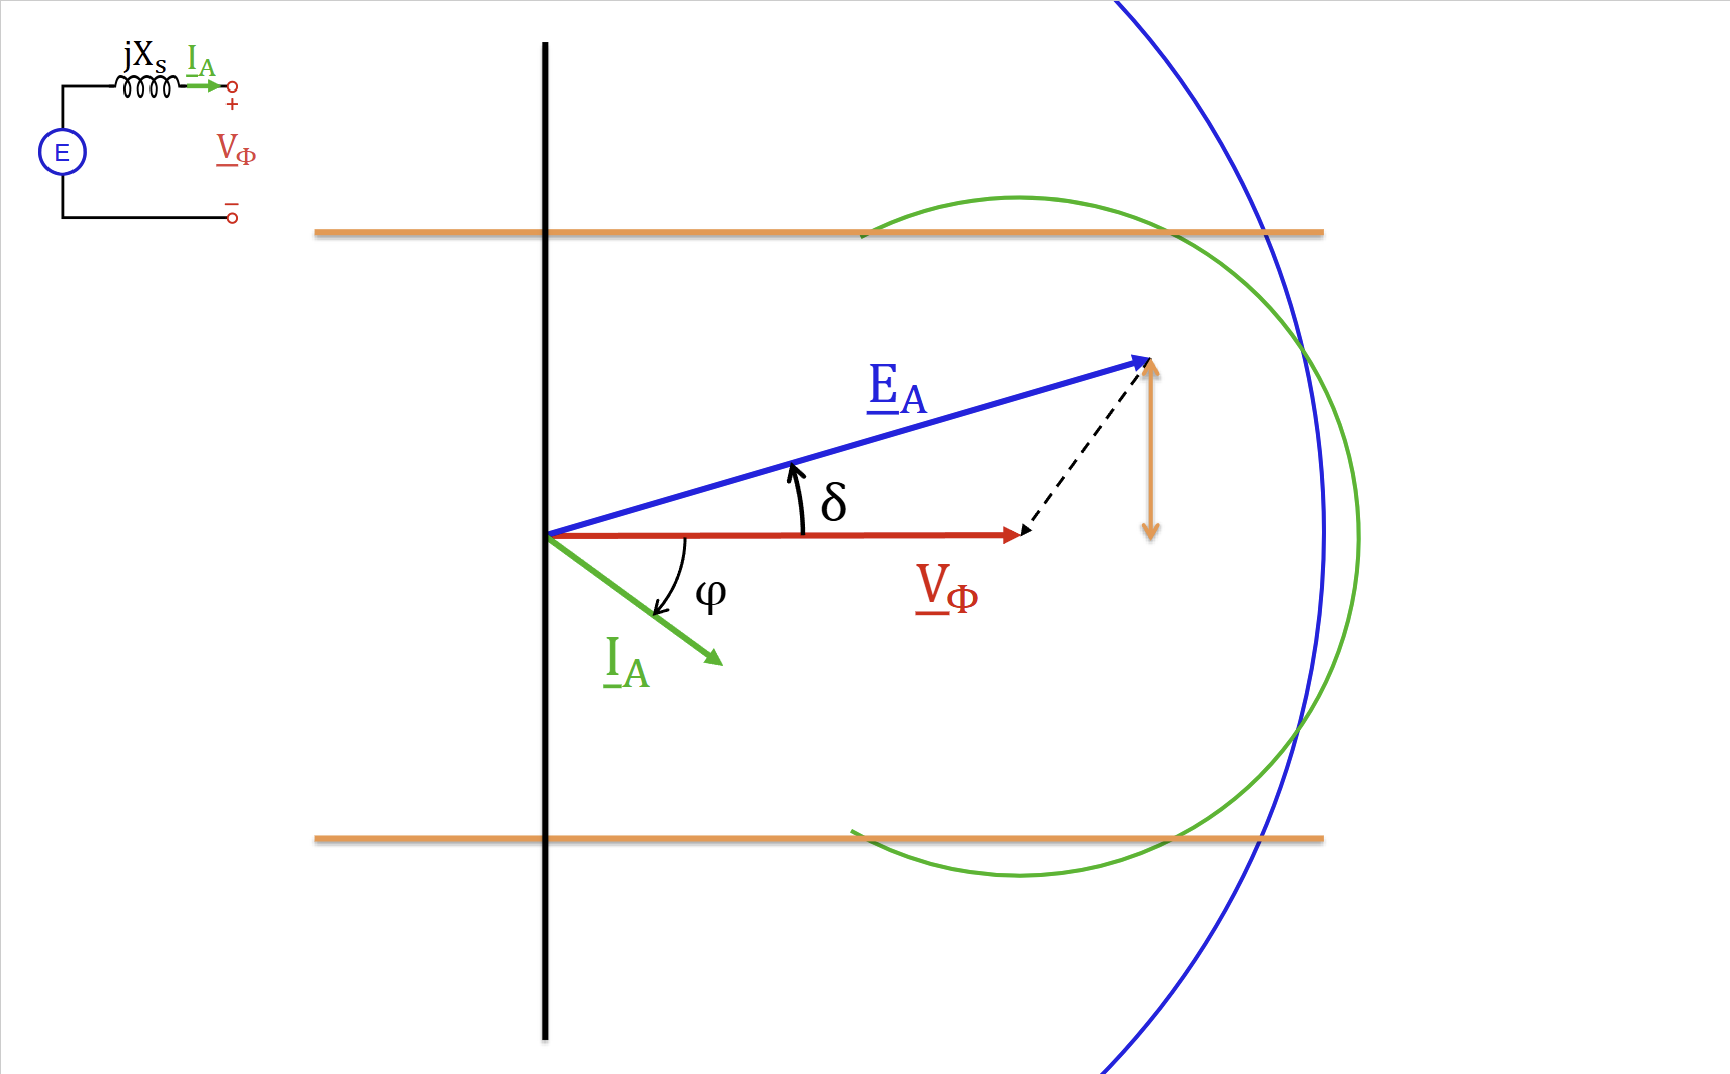
\includegraphics[width=0.7\textwidth]{assets/limietensynchronemachine.png}
  \caption{Ratings van een synchrone machine}
  \label{fig:limietensynchronemachine.png}
 \end{figure}
We hebben een vermogen grens (oranje lijnen) en thermische grenzen (groen en blauwe lijnen). Ook moet natuurlijk nog de lasthoek onder die 90 graden blijven. We beginnen met dit fasediagram waar de fasespanning constant is (star net). Dit fasediagram is trouwens voor 1 van de 3 fases van deze machine getekend, de andere 2 zijn met 120 graden verschoven.
\newline
\newline
$I_A$ mag niet te groot zijn want anders heb je overhitting, deze grens is getekent rond het punt waar de fasespanning daar eindigt want daar begint het gedeelte $j \cdot X_S \cdot I_A$ en dan wordt $X_S$ gewoon geschaald. (Om voor beide gevallen van $j \cdot X_S \cdot I_A$ en $j \cdot X_S \cdot I_S$ te kunnen werken, wordt dit vaak ook $\Delta u$ genoemd)
\newline
\newline
Hetzelfde voor $I_f$, maar hier dan met een grens voor $E_A$ aangeduid omdat dit evenredig is.
\newline
\newline
Er is ook een mechanisch vermogen van de as, dus hoeveel je motor aankan, dit is weergegeven met de oranje horizontale lijnen. De pijl van $E_A$ mag hier niet boven of onder. Meestal is dit de eerste limiet die je bereikt.
\newline
\newline
De zwarte verticale lijn toont tot waar de lasthoek mag gaan. Eigelijk heb je pas vanaf 180 graden dat die toeren overslaat maar voorbij 90 graden loop je het risico voor asynchroonwerking.
\section{Synchrone Motor}
\subsection{Motorwerking}
Nu kijken we naar de motorwerking, we gaan hier uit van een gladde rotor alsook dat de rotor even snel draait als het draaiveld van de stator ($\omega_s$) wat in het echt wel moeilijk is. Even kleine herhaling maar we weten hierbij dus dat de lasthoek negatief is, dus tegengesteld aan de draaizin. Er wordt hier een koppel opgewekt met de volgende formule:
\begin{align*}
    T = k \cdot B_{mut} \cdot B_R \cdot \sin(\delta)
\end{align*}
Bij het equivalent schema gebruiken we nu ook de motorreferentie:
\begin{figure}[H]
  \centering
  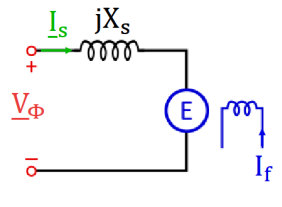
\includegraphics[width=0.3\textwidth]{assets/equivschemamotorref.png}
  \caption{Equivalent schema van een synchrone machine met motorreferentie}
  \label{fig:equivschemamotorref.png}
 \end{figure}
Hierbij mogen we ook niet vergeten dat onze vergelijking nu deze is:
\begin{align*}
    \underline{V}_{\phi} = \underline{E}_A + j \cdot X_S \cdot \underline{I}_S
\end{align*}
Onze stroom $I_S$ loopt nu IN de machine, dus $\Delta u$ heeft een ander teken. Het wordt dus opgeteld bij $E_A$, wat ook zichtbaar is op het fasediagram:
\begin{figure}[H]
  \centering
  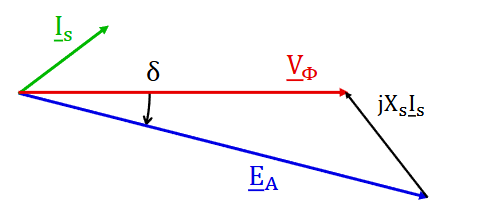
\includegraphics[width=0.5\textwidth]{assets/motorwerkingfasediagram.png}
  \caption{Fasediagram Overbekrachtigde Motor}
  \label{fig:motorwerkingfasediagram.png}
 \end{figure}
We zien hier dus ook dat de stroom $I_S$ loodrecht staat op $\Delta u$ (wat altijd is, ik had het gewoon nog niet eerder gezegd) en ook dat het na ijlt op $\Delta u$ (dit zie je duidelijker als je de aangrijppunten samenneemt, dit is ook altijd)
\subsection{Karakteristieken}
\subsubsection{Koppel-toerentalkarakteristiek}
Het koppel-toerentalkarakteristiek van een synchrone motor ziet er zo uit (met de veronderstelling van een star net!):
\begin{figure}[H]
  \centering
  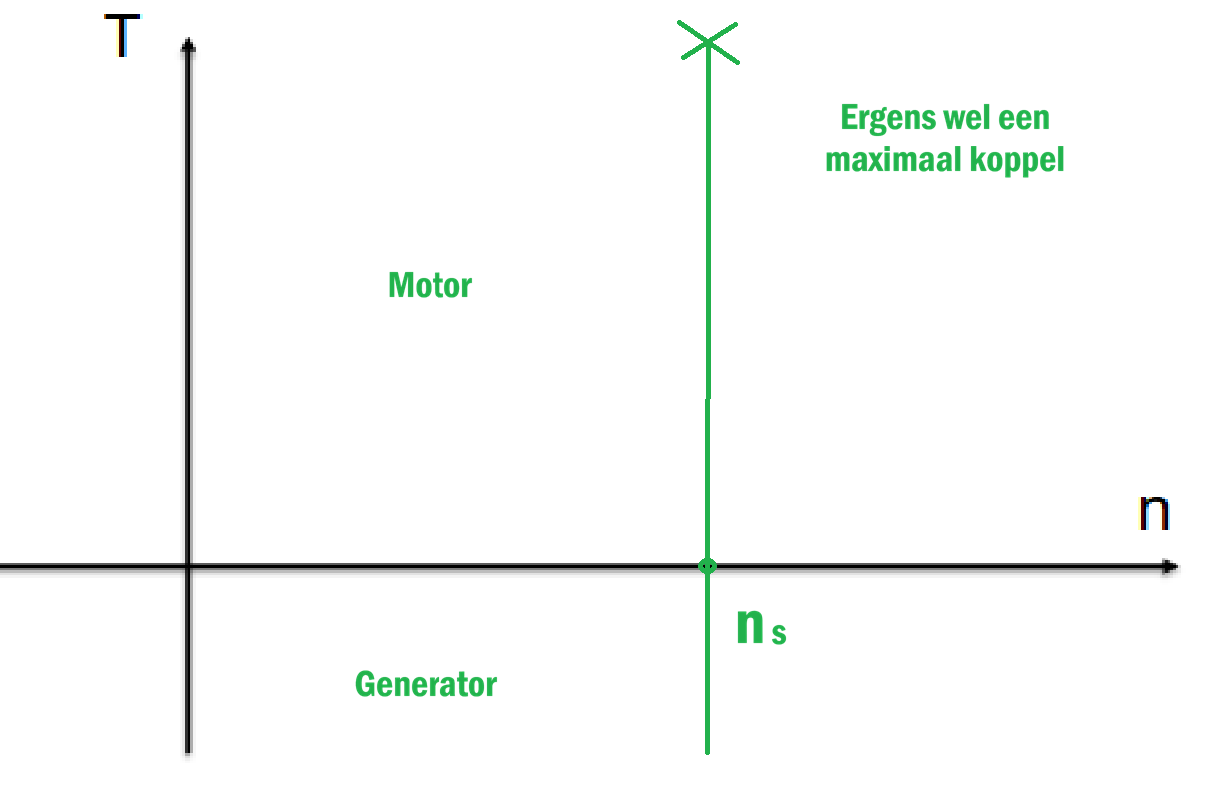
\includegraphics[width=0.5\textwidth]{assets/TNsynchronempotor.png}
  \caption{Koppel-toerentalkarakteristiek van een synchrone motor}
  \label{fig:TNsynchronempotor.png}
 \end{figure}
We zien dat dit gewoon een rechte is op een constante snelheid $n_s$, dit is de ideale machine dus. Het kan in principe onder de n-as gaan want je kan in generator werking zitten. Het grote nadeel hier is dus dat de motor niet zelfstartend is.
\subsubsection{Belastingsvariatie}
Wat gaat de synchrone motor nu doen als de belasting verandert? We nemen hier dus ook star net aan alsook dat de excitatie vast staat (dus gelijke $E_A$). Dus $\omega_s$ constant. Zoals we eerder zagen gaat de afstand tussen $V_{\phi}$ en $E_A$ groter worden als we meer belasten, de lasthoek veranderd dus, dit effect plotten we op de T-$\delta$ karakteristiek.
\begin{figure}[H]
  \centering
  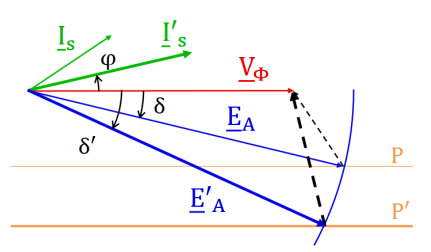
\includegraphics[width=0.5\textwidth]{assets/fasediagrambelastingsvariatiemotor.png}
  \caption{Fasediagram bij belastingsvariatie van een synchrone motor}
  \label{fig:fasediagrambelastingsvariatiemotor.png}
 \end{figure}
We zien dat $\delta$ groter wordt, $\Delta u$ veranderd en dus ook $I_S$ want deze moet loodrecht hierop staan. De stroom wordt hier dus minder capacitief en de grootte veranderd ook wat.
\subsubsection{Koppel-lasthoekkarakteristiek}
Dus de belastingvariatie varieert de lasthoek ook, hier is het bij een motor dus wordt het effect van de lasthoek op het koppel weergegeven met de volgende formule:
\begin{align*}
    T = \frac{3}{\omega_s} \cdot \frac{V_\phi \cdot E}{X_S} \cdot \sin(-\delta_{load})
\end{align*}
Ook weergegeven met deze grafiek:
\begin{figure}[H]
  \centering
  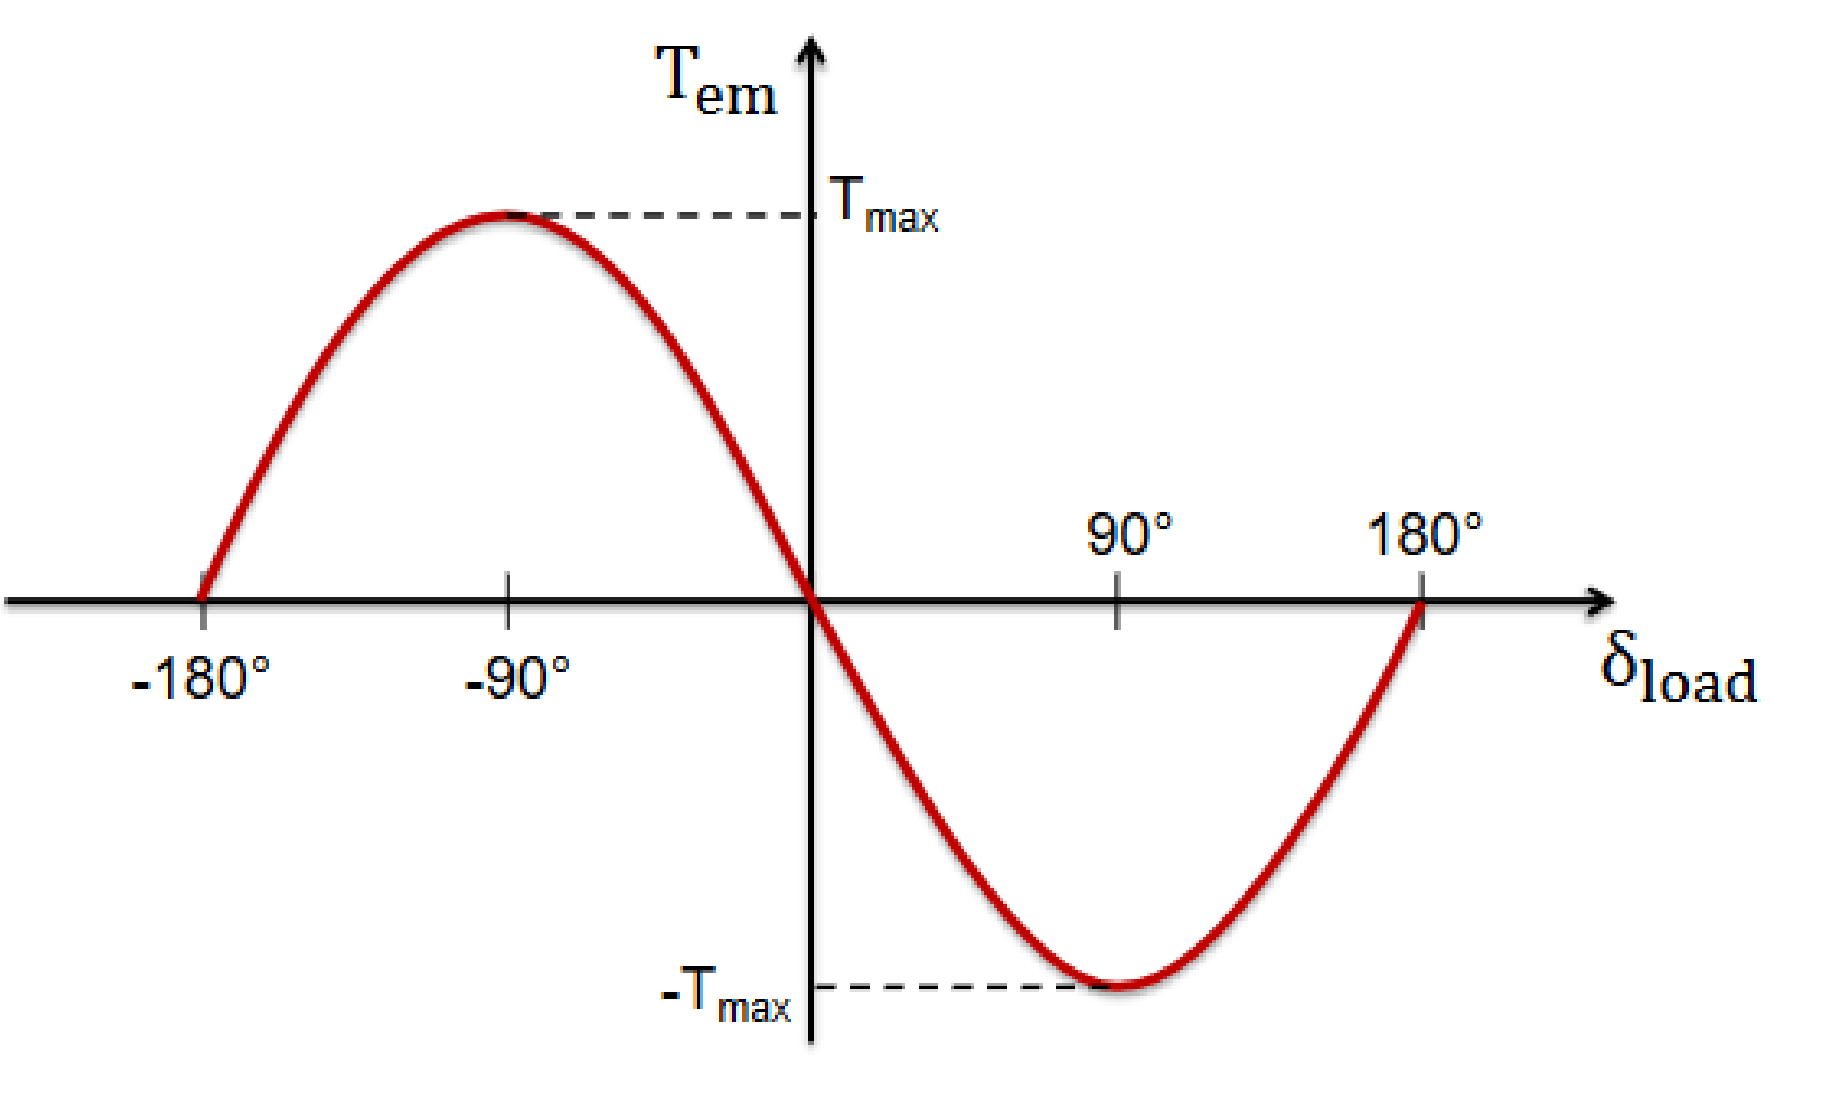
\includegraphics[width=0.5\textwidth]{assets/koppellastkarakteristiekmotor.png}
  \caption{Koppel-lasthoekkarakteristiek van een synchrone motor}
  \label{fig:koppellastkarakteristiekmotor.png}
 \end{figure}
De sinus golf links is voor een motor, die dat de negatieve koppel heeft rechts is voor generator (daar is de lasthoek dus ook groter dan 0).
\subsubsection{Effect van spanningsdip op het koppel}
Dan gaan we nu eens kijken wat er gebeurd als je een plotse spanningsdaling krijg aan de klemspanning (van meer dan 10\%). Via de formule weten we dat het koppel dan zal dalen, waardoor de kans op synchronisatieverlies toeneemt
\begin{figure}[H]
  \centering
  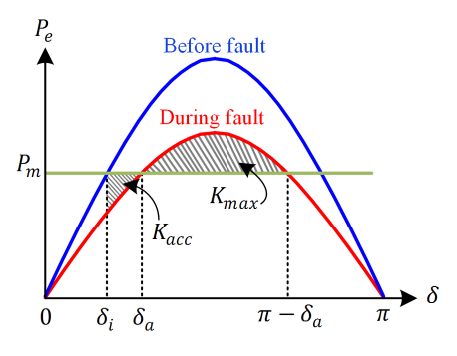
\includegraphics[width=0.5\textwidth]{assets/effectspanningsdip.png}
  \caption{Effect van spanningsdip op het koppel}
  \label{fig:effectspanningsdip.png}
 \end{figure}
In de figuur hierboven zien we dit effect van die spanningsdip, het is hier wel met vermogen weergegeven ma das zo goed als het zelfde want dat is afhankelijk van koppel. We zien de groene lijn, dit is de last die je motor draagt. Er is daar helemaal links een snijpunt met de blauwe curve, dat is je oorspronkelijk werkingspunt. Als er een spanningsdip voorkomt wordt het eigelijk die rode curve, je werkingspunt verschuift dan eigelijk wat waardoor je lasthoek vooral gaat slingeren (en je snelheid ook) zoals een transiënte. Uiteindelijk wordt dan een nieuw werkingspunt gevonden, en dit nieuwe werkingspunt is stabiel als die oppervlakte van $A_1$ kleiner is als die van $A_2$, anders heb je te weinig vermogen en worden toeren gemist en krijg je dus synchronisatie verlies.
\begin{figure}[H]
  \centering
  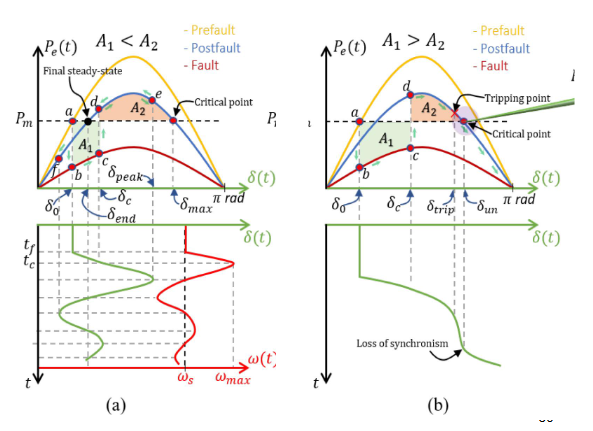
\includegraphics[width=0.5\textwidth]{assets/transienetespannignsdip.png}
  \caption{Transiëne effecten van spanningsdip}
  \label{fig:transienetespannignsdip.png}
 \end{figure}
\newpage
\subsubsection{Effect van excitatie variatie}
Hier gaan we zien wat er gebeurd als je de DC-stroom die het veld bekrachtigd (dus $I_f$) gaat variëren. We houden hier $V_{\phi}$ constant. Wat we zien is dat de interne spanning ook zal stijgen in de vorm van een V-curve als je het plot met de excitatiestroom, een mooie gif hiervan is te vinden op toledo, hier is allesinds een screenshot daarvan:
\begin{figure}[H]
  \centering
  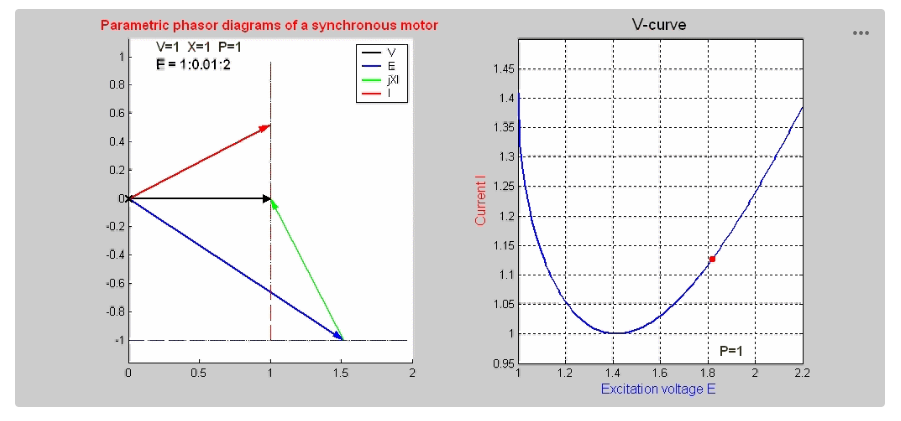
\includegraphics[width=0.6\textwidth]{assets/vcurvevarierenexcitatiestroom.png}
  \caption{V-curve bij variatie van excitatiestroom}
  \label{fig:vcurvevarierenexcitatiestroom.png}
 \end{figure}
Het grote voordeel is dat door dit te variëren je kan bepalen hoe de motor zich gaat gedragen (resistief, inductief of capacitief), het liefst wil je capacitief want dan lever je vermogen aan het net. Resistief heb je trouwens op het minimum van de curve, links daarvan is inductief, rechts daarvan is capacitief. Ook zie je in de figuur dat dit bij een constant vermogen is, dus verschillende V-curves zijn opgesteld voor verschillende vermogens:
\begin{figure}[H]
  \centering
  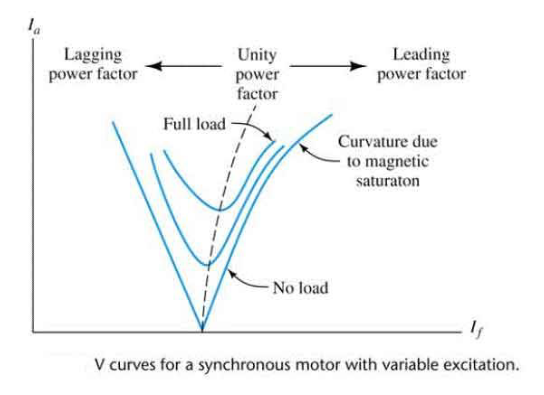
\includegraphics[width=0.5\textwidth]{assets/Vcurvesvoorverschillendevermogens.png}
  \caption{V-curves voor verschillende vermogens}
  \label{fig:Vcurvesvoorverschillendevermogens.png}
 \end{figure}
Die scherpe V-curve helemaal onderaan is de V-curve bij nullast, dit zie je want $I_a$ kan hier 0 zijn, maar niet altijd! Ze kunnen verschillen van nul want deze curve is bij 0 Watt, niet 0A. Ook zien we die zwarte stippelijn een beetje afbuigen, dit is door verzadiging.
\section{Starten van de synchrone motor}
Hoe starten we nu de synchrone motor? Want deze heeft een constante snelheid, die kan alleen draaien op $\omega_s$ terwijl in het begin de snelheid 0 is. Er is niet genoeg koppel dus zoasl we zien in deze T-n karakteristiek van de synchrone machine met de nodige last:
\begin{figure}[H]
  \centering
  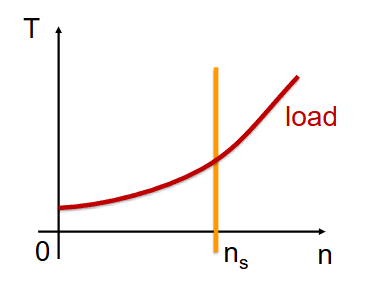
\includegraphics[width=0.3\textwidth]{assets/tnmetnodigdelast.png}
  \caption{Karakteristiek met last}
  \label{fig:tnmetnodigdelast.png}
 \end{figure}
Er zijn verschillende startmethodes die we kunnen gebruiken om de motor toch te doen starten.
\subsection{Het reduceren van elektrische frequentie (Frequentieomvormer)}
We gebruiken een frequentieomvormer om de frequentie geleidelijk aan van 0 tot f te doen stijgen, omdat $n_s = \frac{60f}{p}$. Zo kan de snelheid geleidelijk stijgen. {\color{red}MAAR!}:
\newline
\newline
De spanning E is ook afhankelijk van f met:
\begin{align*}
 E =  \sqrt{2}\cdot \pi \cdot N_c \cdot \phi \cdot f = K \cdot \phi \cdot \omega
\end{align*}
Dus we gaan moeten zien dat als we de frequentie verhogen, we de spanning E ook verhogen, anders is de stroom $I_s$ te groot ($V_{\phi} = E + j \cdot X_S \cdot I_S$), ook gaat het koppel wat lager moeten worden want $T = - \frac{3}{\omega_s} \cdot \frac{V_\phi \cdot E}{X_S} \cdot \sin(\delta)$, dus als $\omega_s$ stijgt, daalt T. Dit is dus een nadeel van deze methode.
\subsection{Hulpmotor gebruiken}
Bij het opstarten met behulp van een hulpmotor gaan we eigenlijk een externe motor gebruiken,
zoals een asynchrone motor die wel kan opstarten vanaf stilstand. Deze gaat dan de synchrone
motor aandraaien, waardoor deze ook gestart geraakt.
We gaan dan eigenlijk eerst de motor opstarten als een generator, waardoor we de motor
kunnen afstemmen op het net, waardoor we de frequentie, spanning en fasehoek juist kunnen
instellen. Hierdoor kunnen we grotere vermogens starten.
\subsection{Damper/Amortisseur windingen gebruiken (Demperkooi)}
Om de synchrone machine te kunnen doen aanlopen, kunnen we ook gebruik maken van een damperwikkeling. Dit is eigenlijk zoals een squirrel cage rotor en gelijkaardig aan de inductiemachine: het zijn kortgesloten koperen staven in de rotor, verbonden door platen. Bij stilstand beweegt het draaiveld relatief ten opzichte van de staven, wat een stroom in de staven induceert die kunnen lopen doordat ze kortgesloten zijn. Samen met het veld wordt hierdoor een kracht uitgeoefend op de staven, die de snelheid van de rotor optrekt zonder dat daar DC-bekrachtiging voor nodig is. Zodra de rotor op synchrone snelheid zit, is er geen relatieve beweging meer, dus ook geen extra geïnduceerde stroom en dus geen verliezen daaraan, de wikkeling ligt dan relatief stil.
\begin{figure}[H]
  \centering
  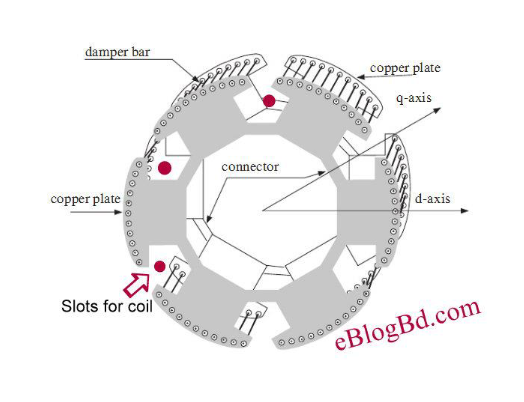
\includegraphics[width=0.5\textwidth]{assets/demperwikkelinge.png}
  \caption{Demperwikkeling in een synchrone machine}
  \label{fig:demperwikkelinge.png}
 \end{figure}
\section{Oefeningen synchrone machines}
\begin{oefenblok}[Oefening 4.6 van Slides]
\textbf{Opgave:}
\newline
The internal generated voltage $E_A$ of a 2-pole, $\Delta$-connected, 60 Hz, three phase synchronous generator is 14.4 kV, and the terminal voltage $V_T$ is 12.8 kV. The synchronous reactance of this machine is 4 $\Omega$, and the armature resistance can be ignored.
\begin{itemize}
 \item a) If the torque angle of the generator $\delta$ is $18^\circ$, how much power is being supplied by this generator at the current time?
 \item b) What is the power factor of the generator at this time?
 \item c) Sketch the phasor diagram under these circumstances.
 \item d) Ignoring losses in this generator, what torque must be applied to its shaft by the prime mover at these conditions?
\end{itemize}
\textbf{Oplossing:}
\newline
We schrijven eerst rap onze gegevens op:
\begin{itemize}
    \item $p = 1$
    \item $f = 60 Hz$
    \item $E_A = 14.4 kV$
    \item $V_T = V_\phi = 12.8 kV$
    \item $X_S = 4 \Omega$
    \item $\delta = 18^\circ$
\end{itemize}
\textbf{a)}
We werken in generatorreferentie dus voor het vermogen gebruiken we de volgende formule ($V_T = V_\phi$ want het is een $\Delta$-verbinding):
\begin{align*}
    P = 3 \cdot \frac{V_\phi \cdot E_A}{X_S} \cdot \sin(\delta) = 3 \cdot \frac{12.8 kV \cdot 14.4 kV}{4 \Omega} \cdot \sin(18^\circ) = 42.7 MW
\end{align*}
\textbf{b)}
Het vermogen dat we net hadden berekend was het elektrisch vermogen, dit kunnen we ook berekenen met de formule:
\begin{align*}
    P = 3 \cdot V_\phi \cdot I_A \cdot \cos(\varphi)
\end{align*}
$I_A$ kunnen we berekenen met de formule:
\begin{align*}
    \underline{V}_{\phi} = \underline{E}_A - j \cdot X_S \cdot \underline{I}_A \\
    \rightarrow j \cdot X_S \cdot \underline{I}_A = \underline{E}_A - \underline{V}_{\phi} \\
    \rightarrow \underline{I}_A = \frac{\underline{E}_A - \underline{V}_{\phi}}{j \cdot X_S}
\end{align*}
Dit kan je invullen in je rekenmachine of grafisch met een fasediagram vinden zodat je krijgt dat:
\begin{align*}
    I_A = \frac{14.4 kV \angle 18^\circ - 12.8 kV \angle 0^\circ}{j \cdot 4 \Omega} = 1.13 kA \angle -11.37^\circ
\end{align*}
En dus de arbeidsfactor gelijk is aan:
\begin{align*}
    \cos(\varphi) = \cos(-11.37^\circ) = 0.981
\end{align*}
\textbf{c)}
Nu simpelweg al deze vectoren tekenen, niet vergeten dat $I_A$ loodrecht staat op $j \cdot X_S \cdot I_A$ en dat $V_\phi = E_A - j \cdot X_S \cdot I_A$.
\begin{figure}[H]
  \centering
  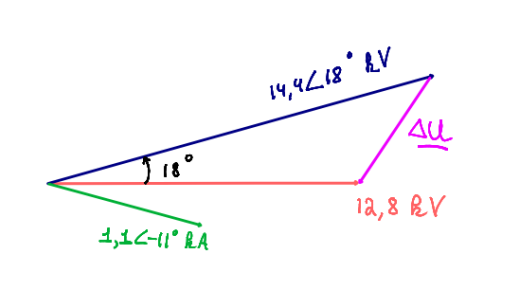
\includegraphics[width=0.5\textwidth]{assets/fasediagramoefening.png}
  \caption{Fasediagram van oefening 4.6}
  \label{fig:fasediagramoefening.png}
 \end{figure}
\textbf{d)}
We mogen verliezen negeren dus geldt dat $P_{elektrisch} = P_{mechanisch}$, dus het koppel dat de as moet leveren is:
\begin{align*}
    P_m = P_{el} = T \cdot \omega_s 
\end{align*}
\begin{align*}
    \rightarrow T = \frac{P_m}{\omega_s} = \frac{42.7 MW}{2 \cdot \pi \cdot 60 Hz} = 113.2 kNm
\end{align*}
\end{oefenblok}
\begin{oefenblok}[Oefening 7.19 van Slides]
\textbf{Opgave:}
\newline
A four-pole, 25 kW, 250 V separately excited DC motor is
mechanically coupled to a threephase four-pole, 25 kVA, 460 V,
cylindrical pole synchronous generator. The DC motor is connected
to a constant 250 V DC supply and the ac generator is connected to
a 460 V fixed voltage, fixed frequency, threephase grid. The
synchronous reactance of the synchronous generator is 6.6 $\Omega$. The
armature resistance of the DC motor is 22 m$\Omega$. All unspecified
losses are to be neglected.
\begin{itemize}
 \item a) If the two machines act as a motor-generator set receiving power from the
DC source and delivering power to the ac grid, what is the internal phase
voltage $E_{SM}$ of the ac machine when it delivers 25kW at unity power factor?
What is the internal voltage (back-emf) of the DC motor?
 \item b) Leaving the field current of the ac machine at the value corresponding to the
condition of part (a), what adjustment can be made to reduce the power
transfer between the two machines to zero? Under this condition of zero
power transfer, what is the armature current of the DC machine? What is
the armature current of the ac machine?
 \item c) Leaving the field current of the ac machine as in parts (a) and (b), what
adjustment can be made to cause the transfer of 25kW from the ac source
to the DC source? Under these conditions, what are the armature current
and internal voltage of the DC machine? What will be the magnitude and
phase of the current in the ac machine? 
\end{itemize}
\textbf{Oplossing:}
\dots ({\color{red}Nog niet aan begonnen})
\end{oefenblok}
\begin{oefenblok}[Oefening 5-3 van Slides]
\textbf{Opgave:}
\newline
A 230-V, 50 Hz, two-pole synchronous motor draws 40 A from the line at unity power factor and full load. Assuming that the motor is lossless, answer the following questions:
\begin{itemize}
 \item a) What is the output torque of this motor? Express the answer in newton-meters.
 \item b) What must be done to change the power factor to 0.85 leading? Explain your answer, using phasor diagrams.
 \item c) What will the magnitude of the line current be if the power factor is adjusted to 0.85 leading?
\end{itemize}
\textbf{Oplossing:}
\dots ({\color{red}Nog niet aan begonnen})
\end{oefenblok}

\begin{oefenblok}[Oefening 5-10 van Slides]
\textbf{Opgave:}
\newline
A synchronous machine has a synchronous reactance of 1.0 $\Omega$ per phase and an armature resistance of 0.1 $\Omega$ per phase. If $E_A = 460 \angle -10^\circ$ V and $V_\phi = 480 \angle 0^\circ$ V, is this machine a motor or a generator? How much power $P$ is this machine consuming from or supplying to the electrical system? How much reactive power $Q$ is this machine consuming from or supplying to the electrical system?
\newline
\textbf{Oplossing:}
\dots ({\color{red}Nog niet aan begonnen})
\end{oefenblok}

\begin{oefenblok}[Oefening 5-17 van Slides]
\textbf{Opgave:}
\newline
A 440-V, 60-Hz, three-phase, Y-connected synchronous motor has a synchronous reactance of 1.5 $\Omega$ per phase. The field current has been adjusted so that the torque angle $\delta$ is $25^\circ$ when the power supplied by the generator is 80 kW.
\begin{itemize}
 \item a) What is the magnitude of the internal generated voltage $E_A$ in this machine?
 \item b) What are the magnitude and angle of the armature current in the machine? What is the motor's power factor?
 \item c) If the field current remains constant, what is the absolute maximum power this motor could supply?
\end{itemize}
\textbf{Oplossing:}
\dots ({\color{red}Nog niet aan begonnen})
\end{oefenblok}
% ==================================================================
\newpage
\chapter{Inductiemachines (Asynchrone Machines)}
\section{Introductie \& Constructie}
Nu gaan we eens kijken naar de inductiemachine, oftewel de asynchrone machine, deze heeft een andere rotor. Eéntje dat we eigelijk eerder zagen; de squirrel cage rotor. Dit is een zeer makkelijk produceerbaar en zeer goedkope rotor, het wordt gemaakt met een gietproces, ook zijn de gebruikskosten van deze motor goedkoper (door bijvoorbeeld minder onderhoud want je hebt hier geen koolstofborstels) dan die van de synchrone maar het heeft wel een slechter rendement. De constructie hebben we eigelijk al wat in sectie 1.2.2 gezien, dus verwijs ik daar naar. Het is gewoon belangrijk dus te weten dat het verschil in die rotor zit, de buitenkant van de machine die wordt gefreesd om aan toleranties te voldoen en het gelijkmatig gewicht wordt ook vaak nog gechecked (dit is nodig voor de praktijk maar hier zijn we niet diep op ingegaan).
\newline
\newline
Een gewikkelde rotor zoals we eerder zagen met sleepringen is ook mogelijk, dit is wel gewoon duurder en moeilijker te produceren dus wordt het minder gedaan.
\section{Werkingsprincipe}
Op de stator gebeurd exact hetzelfde als we eerder zagen bij de synchrone machine, er wordt een draaiveld opgewekt. Een synchroon draaiveld met $\omega_s = \frac{2 \cdot \pi \cdot f}{p}$ en $n_s = \frac{60 \cdot f}{p}$. Ook hier kan de draaizin omgekeerd worden door gewoon 2 fases te verwisselen. Het is bij de rotor dat het speciale ding gebeurd.
\newline
\newline
Bij de rotor is het wat anders, je hebt hier dus die kooirotor die stil staat maar een draaiend magnetisch veld passeert er rond. Als jij als waarnemer op het draaiveld staat, dan zie je eigelijk een bewegende geleider in een magnetisch veld, dus wordt er een spanning geïnduceerd, en doordat dus die kooirotor kortgesloten is, vloeit er een stroom dat zich dus ook in een magnetisch veld bevindt. Dit wekt een lorentzkracht op de rotorstaven op wat dus het koppel veroorzaakt dat de rotor doet draaien. Van zodra de rotor op synchrone snelheid van het draaiveld staat dan wordt er geen spanning meer geïnduceerd, want relatief is er geen bewegende geleider in een magnetisch veld meer. Dus is er geen koppel op synchrone snelheid.
\begin{figure}[H]
  \centering
  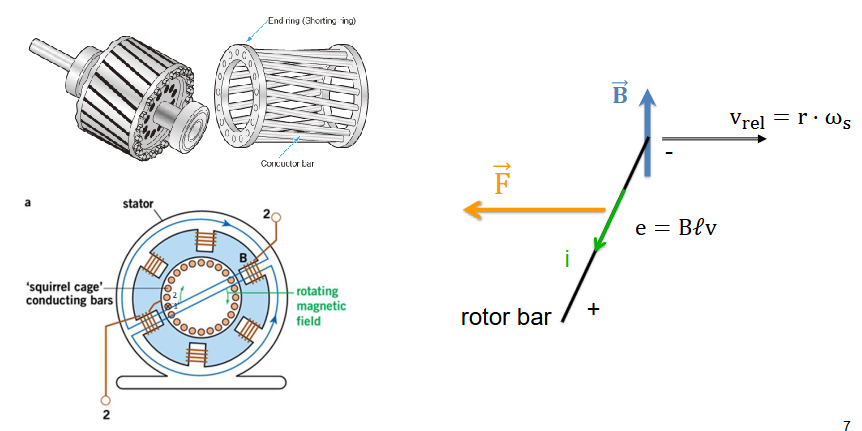
\includegraphics[width=0.6\textwidth]{assets/inductiemachinerotor.png}
  \caption{Rotor inductiemachine}
  \label{fig:inductiemachinerotor.png}
 \end{figure}
De wetten die dit dus allemaal mogelijk maakten zijn:
\begin{itemize}
 \item Wet van Faraday Lenz: $e = B \cdot l \cdot v$
 \item Wet van Lorentz: $F = B \cdot l \cdot I$
 \item Wet van Ohm: $i = \frac{e}{R}$
 \item Wet van Newton: $\sum T = J \cdot \alpha$ ($J$ = traagheidsmoment, $\alpha$ = hoekversnelling)
\end{itemize}
\subsection{Slip}
Bij de inductiemachine komt de term 'slip' ook vaak aan bod, dit is omdat de spanning enkel geïnduceerd wordt als er een snelheidsverschil is tussen het veld en de rotor en de slip wordt letterlijk geclassificeerd als \textit{het snelheidsverschil tussen het draaiveld en de rotor.} Daarom kan de slip wiskundig als volgt ook beschreven worden:
\begin{align*}
 s = \frac{n_s - n}{n_s} \cdot 100\% = \frac{\omega_s - \omega}{\omega_s} \cdot 100\%
\end{align*}
Typisch is de slip rond de 3\%, 10\% wordt al als veel beschouwd. Het is eigelijk een andere uitdrukking voor snelheid, daarom kan het ook geplot worden met het koppel in een koppel-slip karakteristiek zoals in volgende figuur:
\begin{figure}[H]
  \centering
  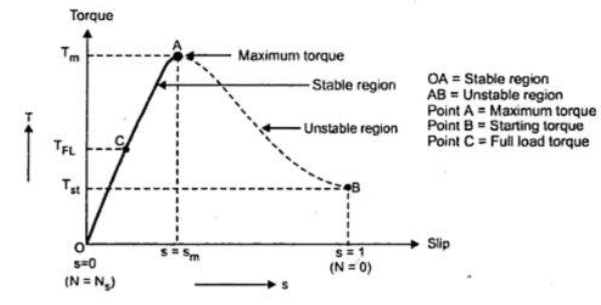
\includegraphics[width=0.6\textwidth]{assets/koppelslip.png}
  \caption{Koppel-slip karakteristiek van een inductiemachine}
  \label{fig:koppelslip.png}
 \end{figure}
We zien hier dat we bij een slip van 0 geen koppel hebben, dit is logisch want op dat moment draaien we aan synchrone snelheid waardoor dus geen geïnduceerde spanning is. Bij een slip van 1 hebben we eigelijk gewoon een stilstaande rotor, het draaiveld van de stator draait hier wel nog. Voor kleine slippen zoals we zien is er eigelijk een lineair verband met het koppel.
\subsection{Rotorveld}
Aangezien er een stroom in de rotor is zorgt deze ook voor een magnetisch veld via de wet van Ampère. Dit veld een een beetje effect op het resulterend draaiveld, maar hoe groter deze stroom hoe groter dat effect, dit is dus eigelijk zoals ankerreactie. Door de slip is er een verschil in snelheid, we zeggen hier dat het draaiveld aan 1500 tr/min draait en de rotor aan 1480 tr/min.
\subsubsection{Buitenstaande waarnemen (stator)}
Als je als buitenstaande waarnemer gaat kijken naar de inductie machine dan ziet die gewoon alle stromen van in de volgende figuur draaien aan een snelheid van 1500 tr/min, terwijl de rotorstroom $I_R$ zich in de rotor bevind, dit is omdat het geïnduceerd wordt door dat draaiveld dat het dan eigelijk iets sneller draait als de rotor zelf.
\begin{figure}[H]
  \centering
  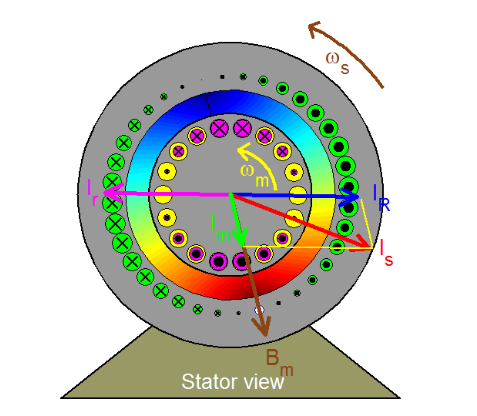
\includegraphics[width=0.4\textwidth]{assets/statorviewinductiemachine.png}
  \caption{Stator view van een inductiemachine, buitenstaander waarnemer}
  \label{fig:statorviewinductiemachine.png}
 \end{figure}
\subsubsection{Synchronous view (jij rijdt mee op het draaiveld)}
Als we nu als waarnemer OP de machine gaan, eigelijk mee met het draaiveld, dan is $\omega = 0$, het draaiveld is stil vanuit ons standpunt, maar sinds de rotor dat tempo niet haalt gaat het eigelijk traag lijken weg te glijden, waardoor de stroom in de rotorstaven traag varieert. Dit is dus gelinkt aan die slip, die stroom is een geïnduceerde AC stroom dat niet aan 50Hz is maar trager dan het draaiveld.
\begin{figure}[H]
  \centering
  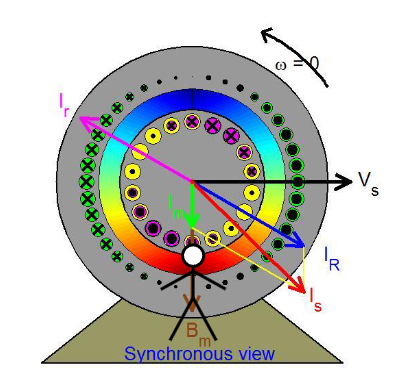
\includegraphics[width=0.4\textwidth]{assets/synchronoyusviewinductiemachine.png}
  \caption{Synchronous view van een inductiemachine, waarnemer die mee rijdt op het draaiveld}
  \label{fig:synchronoyusviewinductiemachine.png}
 \end{figure}
\subsubsection{Rotor view (jij rijdt mee op de rotor)}
Als we nu als waarnemer op de rotor gaan, lijkt het draaiveld aan 20 tr/min te passeren, dus aan $\omega_{sl} = 20 tr/min$, dit is die slip. Als we dit omzetten naar frequentie geeft dit exact volgende relatie:
\begin{align*}
    f_r = s \cdot f_s
\end{align*}
De rotor frequentie is een lage frequentie, dus niet 50Hz, dit is een belangrijke formule om te onthouden.
\begin{figure}[H]
  \centering
  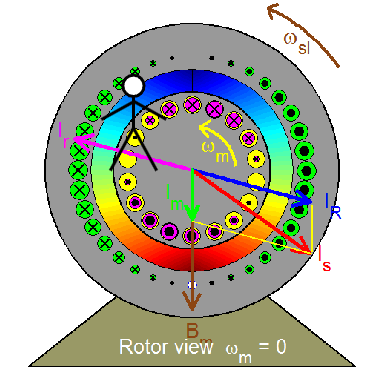
\includegraphics[width=0.4\textwidth]{assets/rotorviewinductiemachine.png}
  \caption{Rotor view van een inductiemachine, waarnemer die mee rijdt op de rotor}
  \label{fig:rotorviewinductiemachine.png}
 \end{figure}
\subsection{Kenplaat oefening}
Dit thema is een beetje messy als het neer komt op de oefeningen, ze zijn niet zomaar allemaal vanachter op het eind van dit thema, ik ga de meeste hiervan dus tussen de theorie plaatsen in de zelfde volgorde als hoe ze in de les aan bod kwamen. Ik raad aan om ze ook zo te maken in plaats van te wachten tegen dat je het hoofdstuk van inductiemachines af hebt want dit is veel.
\begin{oefenblok}[Oefening Kenplaat Inductiemachine]
\textbf{Opgave:}
\begin{figure}[H]
  \centering
  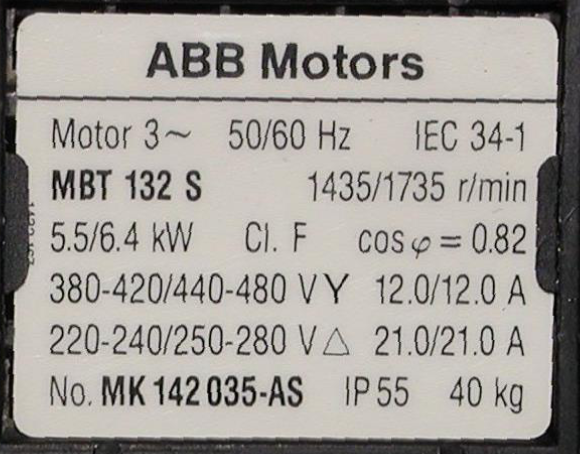
\includegraphics[width=0.5\textwidth]{assets/kenplaatoefeninginductiemachine.png}
  \caption{Kenplaat oefening inductiemachine}
  \label{fig:kenplaatoefeninginductiemachine.png}
 \end{figure}
\begin{itemize}
 \item a) Determine: p, $n_s$, $s_{nom}$, $\eta_{nom}$, $T_{nom}$
 \item b) The load torque is half of the nominal torque. Determine the output power.
 \item c) The rotor is driven (i.e. generator) with a torque of 25Nm. Determine the rotor speed.
\end{itemize}
\textbf{Oplossing:}
\newline
\textbf{a)}
\newline
Er is geen ronde synchrone snelheid gegeven, er is wel gegeven dat het nominale toerental $n_{nom} = 1435 tr/min$ is. Dit kan alleen overkomen met een 4 polige machine want deze heeft een synchrone snelheid van 1500 tr/min. Dit toerental van 1435 komt overeen met een frequentie van 50Hz, dus die 1500 kunnen we ook dubbel checken met:
\begin{align*}
    n_s = \frac{60 \cdot f}{p} = \frac{60 \cdot 50 Hz}{4} = 750 tr/s = 1500 tr/min
\end{align*}
De nominale slip vinden we dan met de eerder geziene formule:
\begin{align*}
    s_{nom} = \frac{n_s - n_{nom}}{n_s} = \frac{1500 - 1435}{1500} = 0.0433 = 4.33\%
\end{align*}
Het nominaal rendement vinden we met de formule:
\begin{align*}
    \eta_{nom} = \frac{P_{out}}{P_{in}} = \frac{P_{mech}}{P_{el}}
\end{align*}
Het mechanisch vermogen kan afgelezen worden van de kenplaat en bedraagt 5.5 kW. Het elektrisch vermogen kunnen we berekenen met de formule:
\begin{align*}
    P_{el} = \sqrt{3} \cdot V_L \cdot I_L \cdot \cos(\varphi)
\end{align*}
$V_L$ en $I_L$ kunnen we aflezen, we gaan dit doen voor Ster. Aangezien de lijnspanning een range heeft pakken we het gemiddelde hiervan (400V) en de lijnstroom bij ster bedraagt 12A. De arbeidsfactor kunnen we ook aflezen (0.82). Invullen geeft:
\begin{align*}
    P_{el} = \sqrt{3} \cdot 400 V \cdot 12 A \cdot 0.82 = 6.82 kW
\end{align*}
Het nominaal rendement is dus:
\begin{align*}
    \eta_{nom} = \frac{5.5 kW}{6.82 kW} = 0.806 = 80.6\%
\end{align*}
Het nominaal koppel kunnen we berekenen met de formule:
\begin{align*}
    T_{nom} = \frac{P_{mech}}{\omega_{nom}} = \frac{5.5 kW}{2 \cdot \pi \cdot \frac{1435 tr/min}{60}} = 36.7 Nm
\end{align*}
\textbf{b)}
\newline
Als we het koppel van de last gaan halveren, gaat bij benadering het vermogen ook halveren, maar het is dus eigelijk fout om het zo te doen want $\omega$ vernaderd ook en er zal dus minder slop nodig zijn omdat gehalveerd koppel te leveren. Dit gaan we nu ook proberen na gaan.
\newline
\newline
Wat we gaan doen is kijken naar de T-n grafiek, want in de buurt van $n_s$ is deze kromme eigelijk een rechte lijn (zoals bij de T-s grafiek). 2 punten van deze rechte kennen we, namelijk het punt (n = 1435; T = 36,7) en (n = 1500; T = 0). Via interpolatie vinden we zo welk toerental bij het gehalveerd koppel hoort. Hiermee vinden we juiste $\omega$ en zo het juiste vermogen bij een gehalveerd koppel:
\begin{figure}[H]
  \centering
  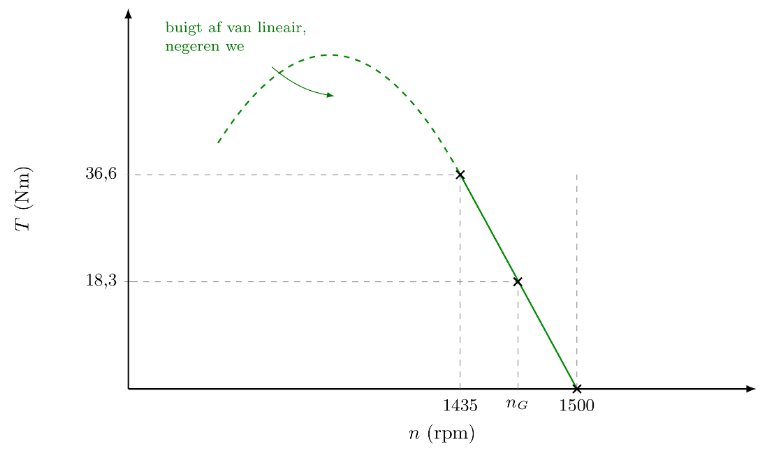
\includegraphics[width=0.6\textwidth]{assets/AIgeneratedgrafieklineairgebiedTn.png}
  \caption{Lineair verloop van T-n karakteristiek in het gebied van nominale snelheid (AI gegenereerd maar is juist)}
  \label{fig:AIgeneratedgrafieklineairgebiedTn.png}
 \end{figure}
\begin{align*}
 n_G = n_1 + \frac{T_G - T_1}{T_2 - T_1} \cdot (n_2 - n_1) = 1435 + \frac{18.35 - 36.7}{0 - 36.7} \cdot (1500 - 1435) = 1467 tr/min
\end{align*}
Hiermee kunnen we het mechanisch vermogen berekenen:
\begin{align*}
    P_{mech} = T_G \cdot \omega_G = 18.35 Nm \cdot 2 \cdot \pi \cdot \frac{1467 tr/min}{60} = 2.82 kW
\end{align*}
Dit is inderdaad ongeveer de helft van het nominaal vermogen, maar niet exact want de snelheid is ook veranderd.
\newline
\textbf{c)}
Nu wordt de rotor aangedreven met een koppel van 25Nm, dit is dus generatorwerking. Dit is een negatief koppel op de grafiek maar gaat de snelheid trager of sneller zijn dan de synchrone snelheid? Wel, een aangedreven rotor die generator wordt, kan alleen als hij sneller draait dan het draaiveld dus het is groter, we kunnen de lineaire relatie dan onder de n-as doortrekken en de snelheid berekenen bij -25Nm:
\begin{align*}
    n_C = n_1 + \frac{T_C - T_1}{T_2 - T_1} \cdot (n_2 - n_1) = 1435 + \frac{-25 - 36.7}{0 - 36.7} \cdot (1500 - 1435) = 1544 tr/min
\end{align*}
\begin{figure}[H]
  \centering
  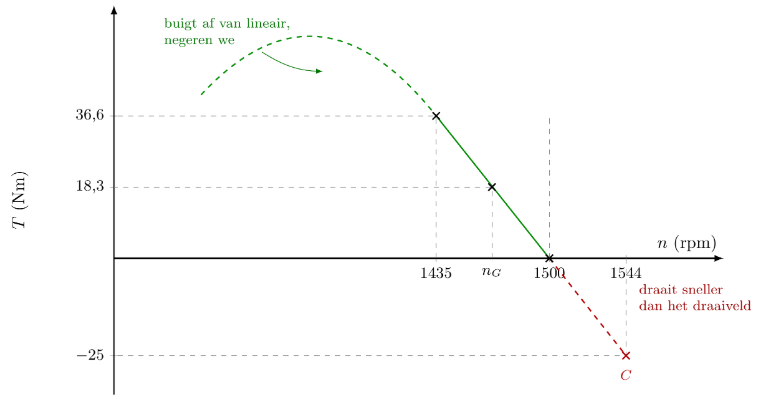
\includegraphics[width=0.6\textwidth]{assets/AIgeneratedgrafieklineairgebiedgenerator.png}
  \caption{Lineair verloop van T-n karakteristiek in het gebied van generatorwerking (AI gegenereerd maar is juist)}
  \label{fig:AIgeneratedgrafieklineairgebiedgenerator.png}
 \end{figure}
\end{oefenblok}
\subsection{Nominaal werkingspunt}
In volgende figuren zien we verschillende karakteristieken met hun aangeduidde nominale werkingspunten:
\begin{figure}[H]
  \centering
  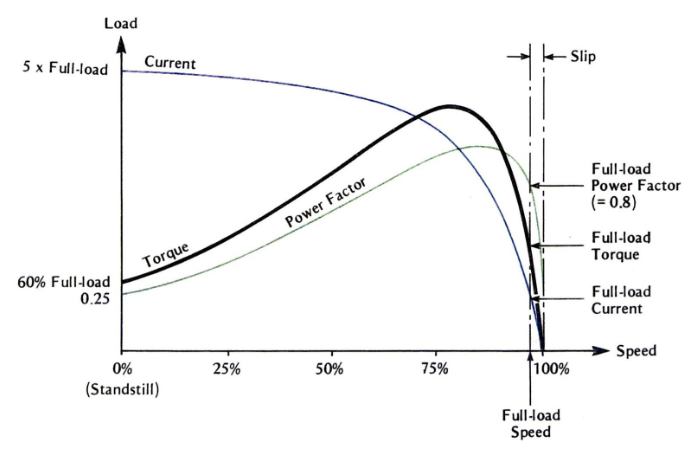
\includegraphics[width=0.6\textwidth]{assets/nominalewerkingspuntkarakteristieken.png}
  \caption{Stroom, koppel en arbeidsfactor karakteristiek}
  \label{fig:nominalewerkingspuntkarakteristieken.png}
 \end{figure}
We zien dat bij vollast de arbeidsfactor goed is als die rond de 0.8 ligt. Aan de grafiek zien we ook het grootste nadeel van de inductie motor; namelijk de hoge startstroom.
\section{Equivalent schema}
Voor het opstellen van het equivalent schema van de inductiemachine gaan we niet van 0 beginnen, we gaan een analogie zoeken en hiernaar toe aanpassen. We gebruiken hier die van de transformator want eigelijk is de inductiemachine een soort van transfo want we hebben hier ook eigelijk een spanning dat wordt geïnduceerd van de ene kant naar de andere kant. Hier is dit dan met een stator en een rotor i.p.v. een primaire en secundaire wikkeling. We gaan hierbij van uit van een symmetrisch net, en ook van een sinusoïdaal magnetisch veld in de luchtspleet. Het schema dat we opstellen is hier ook een éénfasig equivalent, let hier mee dus op want een inductie motor is 3-fasig. Tussen de transfo en de inductie machine zijn echter 3 grote verschillen:
\begin{itemize}
    \item De rotor is kortgesloten, dus er is geen spanning dat we kunnen meten aan de rotor, dit is dus een verschil met de transfo. Hierdoor kan er wel een stroom $I_r$ lopen zonder dat er iets extern aangesloten moet worden, het loopt door de geînduceerde $E_R$ door de impedantie van de rotor
    \item Er werkt een andere frequentie in de rotor dat verschilt van de stator
    \item De spoel $L_m$ (magnetiseringstroom) is veel kleiner hier, waardoor we veel meer nullaststroom krijgen. (Bij een motor is dit niet zo een groot probleem, bij een transfo wel)
\end{itemize}
\begin{figure}[H]
  \centering
  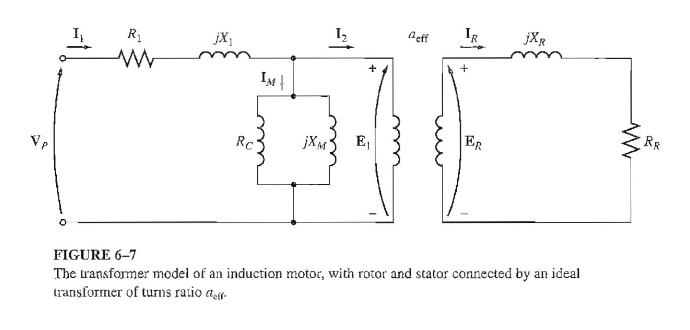
\includegraphics[width=0.8\textwidth]{assets/transfoanalogieinductiemachine.png}
  \caption{Transfo analogie inductiemachine}
  \label{fig:transfoanalogieinductiemachine.png}
 \end{figure}
Het equivalent schema van de inductiemachine is dus als volgt:
\begin{figure}[H]
  \centering
  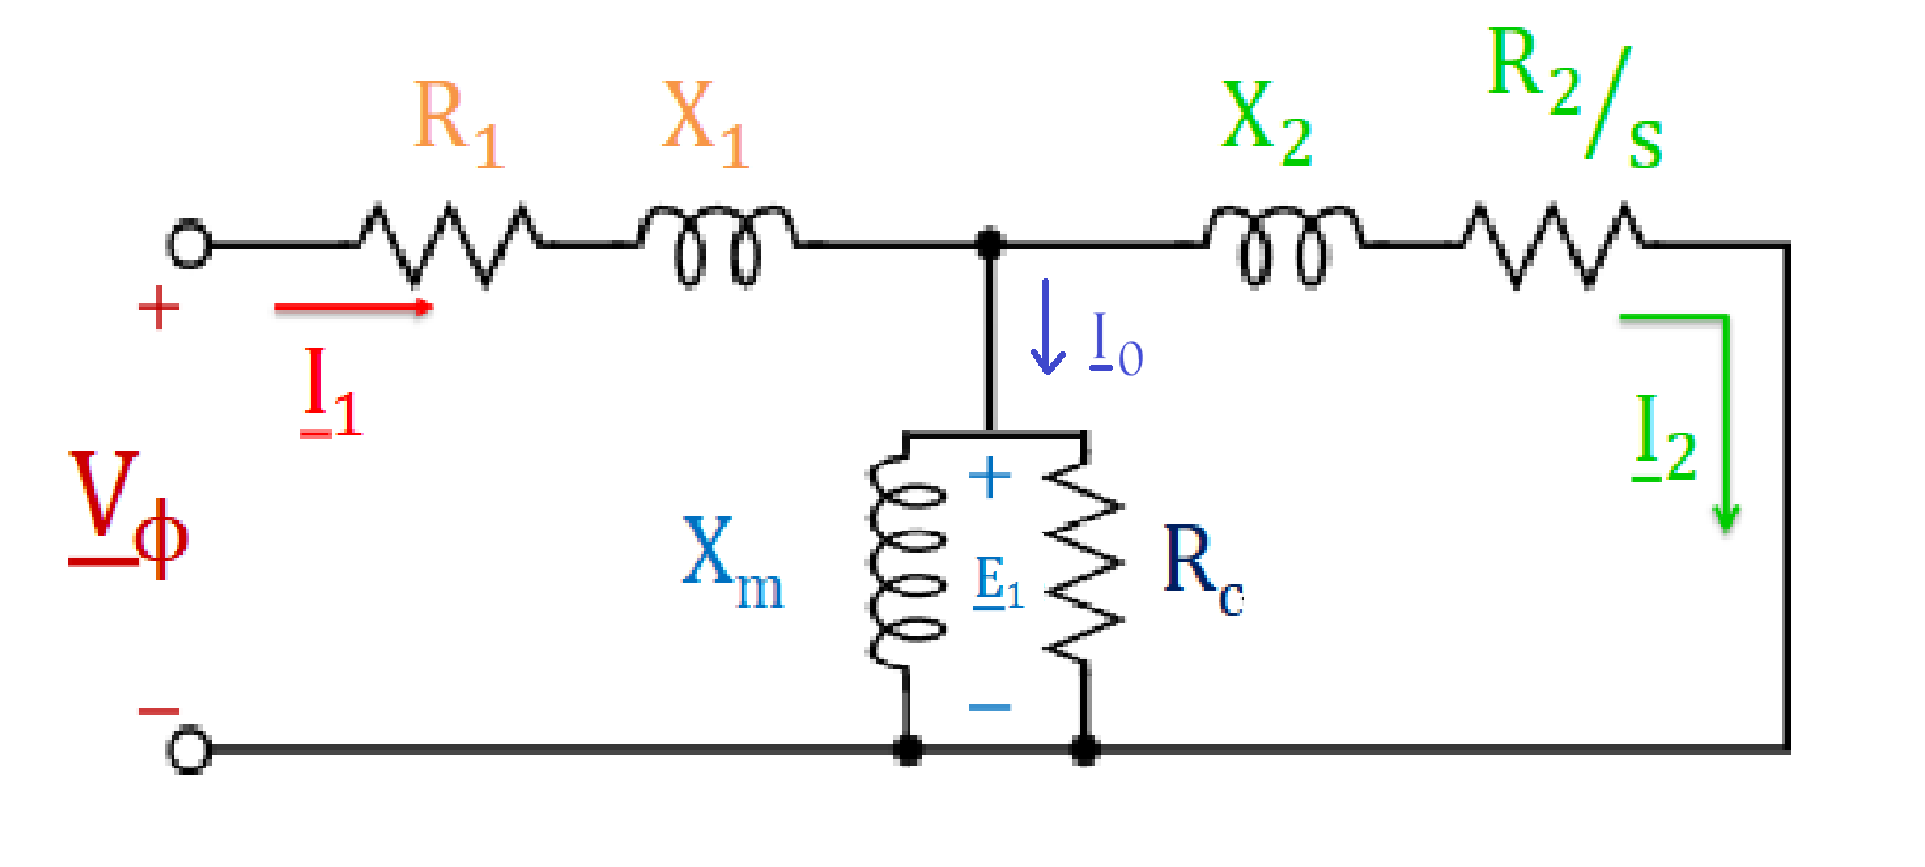
\includegraphics[width=0.8\textwidth]{assets/equivalentschemainductiemotor.png}
  \caption{Equivalent schema inductiemachine}
  \label{fig:equivalentschemainductiemotor.png}
 \end{figure}
Hierbij is:
\begin{itemize}
 \item \textbf{$R_1$} de fysieke weerstand van de statorwikkeling (koperverlies)
 \item \textbf{$X_1$} de lekreactantie van de stator, dit gaat door de stator en bereikt (niet volledig) de rotor
 \item \textbf{$R_C$} het model van de ijzerverliezen (kern), dit is geen echte weerstand, gewoon een model om deze verliezen elektrisch voor te stellen! (Wervel en hysteresis eigelijk)
 \item \textbf{$X_m$} de mutuele/magnetiserende reactantie
 \item \textbf{$E_1$} de interne spanning over de parallele tak van $R_C$ en $X_m$
 \item \textbf{$X_2$} de lekreactantie van de rotor, dit gaat door de rotor en bereikt (niet volledig) de stator
 \item \textbf{$R_2$} de fysieke weerstand van de rotorwikkeling (koperverlies) (Er staat wel $\frac{R_2}{s}$ in het schema, hier kom ik zometeen op terug)
 \item \textbf{$I_1$} de stroom door de statorwikkeling
 \item \textbf{$I_2$} de stroom door de rotorwikkeling
 \item \textbf{$I_0$} de nullaststroom, dit is de stroom die loopt door $R_C$ en $X_m$, deze kan tot 30\% van de nominale stroom zijn, want de luchtspleet zorgt dat we veel stroom nodig hebben
\end{itemize}
Liefst hebben we $X_1$ en $X_2$ zo klein mogelijk en $X_m$ zo groot mogelijk (logisch, minder verlies en minder stroom), bij de transfo gelde ook dat R1 en R2 gelijkmatig verdeeld werden maar dit is nu niet meer zo aangezien da stator en de rotor uit verschillend materiaal bestaan.
\subsection{Waarom staat er $\frac{R_2}{s}$ i.p.v. $R_2$?}
Dit is het lastigste stuk van het schema, dus we bouwen het stap voor stap op.

Het probleem: de rotor werkt niet aan de statorfrequentie $f_s$, maar aan de rotorfrequentie $f_r = s \cdot f_s$ (bv. 50Hz bij stilstand, maar slechts 1 à 2Hz bij normaal bedrijf met een kleine slip). We willen echter maar 1 schema tekenen, op 1 frequentie (die van de stator). Daarom moeten we de rotorvergelijking eerst herschrijven.

Aan de eigen (rotor)frequentie geldt gewoon de wet van Ohm over de kortgesloten rotorlus:
\begin{align*}
    E_R = R_R \cdot I_R + jX_R \cdot I_R
\end{align*}
Hierbij is $X_R = s \cdot X_{R0}$, met $X_{R0}$ de rotorreactantie bij stilstand (dus bij 50Hz, $s=1$). Ook $E_R$ zelf is rechtevenredig met de slip: $E_R = s \cdot E_{R0}$ (logisch, want $e = B\ell v$: hoe groter de relatieve snelheid tussen rotor en draaiveld, hoe groter de geïnduceerde spanning).

Vullen we dit in en delen we alles door $s$, dan krijgen we:
\begin{align*}
    s \cdot E_{R0} = R_R \cdot I_R + j s X_{R0} \cdot I_R \quad\Rightarrow\quad E_{R0} = \left(\frac{R_R}{s} + jX_{R0}\right) \cdot I_R
\end{align*}
En daar komt die $\frac{R_2}{s}$ dus vandaan: het is geen aparte fysische grootheid, het is gewoon het resultaat van die deling door $s$, nodig om het frequentieverschil tussen rotor en stator weg te werken zodat we alles op de statorfrequentie kunnen tekenen. $\frac{R_2}{s}$ in het equivalent schema schrijven compenseert dus voor die verschillde frequenties. Het is dus eigelijk gelijk aan:
\begin{align*}
   \frac{R_2}{s} = R_2 + (\frac{1-s}{s}) \cdot R_2 = \underbrace{R_2 + {R'}_{load}}_{\text{in serie}}
\end{align*}
Die $R'_{load}$ is dus de weerstand die de rotor moet overwinnen om het koppel te leveren, en die is groter naarmate de slip kleiner wordt (want dan draait de rotor sneller, dus moet hij meer kracht leveren). Bij stilstand ($s=1$) is er geen extra weerstand, bij synchrone snelheid ($s=0$) is de weerstand oneindig groot (want dan kan er geen stroom meer lopen in de rotor).
\begin{warningbox}[Hier zijn het fasegrootheden, geen lijn grootheden!]
    Alle grootheden weergegeven in het equivalent schema zijn fase grootheden, niet lijn grootheden. Bij kenplaten wordt wel alles in lijn grootheden weergegeven, dus let hier goed op bij het oplossen van oefeningen.
\end{warningbox}
\section{Vermogensbalans}
Nu gaan we kijken naar het vermogen balans, en dus ook waar precies in de inductiemachine alle verliezen bevinden. We bespreken ook de formules, we gaan dit allemaal doen aan de hand van een soort van Sankey-diagram zoals te zien in de volgende figuur: 
\begin{figure}[H]
\centering
\begin{tikzpicture}[
    node distance=0.25cm,
    block/.style={single arrow, draw=black, thick, minimum height=1.5cm,
                  minimum width=1.7cm, single arrow head extend=0.25cm,
                  font=\bfseries, align=center, inner sep=2pt},
    stage/.style={circle, draw=black, thick, fill=violet!60,
                  minimum size=1.6cm, font=\bfseries\footnotesize, align=center},
    formula/.style={align=center, font=\small},
    lossarrow/.style={single arrow, draw=black, thick, fill=red!35,
                       minimum height=0.9cm, minimum width=0.35cm,
                       single arrow head extend=0.12cm, rotate=-90},
]

\node[block, fill=orange!55] (Pin) {$P_{in}$};
\node[stage, right=of Pin] (stator) {Stator};
\node[block, fill=blue!30, right=of stator] (Ps) {$P_{S}$};
\node[stage, right=of Ps] (rotor) {Rotor};
\node[block, fill=green!40, right=of rotor] (Pconv) {$P_{conv}$};
\node[stage, right=of Pconv] (shaft) {Shaft};
\node[block, fill=green!40, right=of shaft] (Pout) {$P_{mech}$};

\node[formula, above=0.35cm of Pin] {$\sqrt{3}V_TI_T\cos\varphi = 3V_\phi I_1\cos\varphi$\\$\Vert$};
\node[formula, above=0.35cm of Ps] {$3\dfrac{R_2}{s}I_2^2$\\$\Vert$};
\node[formula, above=0.35cm of Pconv] {$T_{ind}\cdot\omega$\\$\Vert$\\$3R_2\left(\dfrac{1-s}{s}\right)I_2^2$};
\node[formula, above=0.35cm of Pout] {$T_{load}\cdot\omega$\\$\Vert$};

\node[lossarrow] (lcus) at ($(stator.south)+(-0.6,-0.7)$) {};
\node[formula, below=0.45cm of lcus] {$P_{Cu,s}$\\$\Vert$\\$3I_1^2R_1$};

\node[lossarrow] (lfe) at ($(stator.south)+(0.6,-0.7)$) {};
\node[formula, below=0.45cm of lfe] {$P_{Fe}$\\$\Vert$\\$3\dfrac{E_1^2}{R_C}$};

\node[lossarrow] (lwr) at ($(rotor.south)+(0,-0.7)$) {};
\node[formula, below=0.45cm of lwr] {$P_{Cu,r}$\\$\Vert$\\$3I_2^2R_2 = s \cdot P_S$};

\node[lossarrow] (lfw) at ($(shaft.south)+(0,-0.7)$) {};
\node[formula, below=0.45cm of lfw] {$P_{wr} + P_w + P_{str}$};

\end{tikzpicture}
\caption{Vermogensbalans van de inductiemachine}
\label{fig:vermogensbalans}
\end{figure}
Wat we hier zien is dat we starten bij het elektrisch vermogen $P_{el}$ dat in de stator wordt geleverd, dit is het vermogen dat we dus van het net halen. In de stator zijn er wel een paar verliezen, namelijk de ijzerverliezen $P_{Fe}$ en de koperverliezen $P_{Cu,s}$. Het vermogen dat overblijft wordt overgedragen naar de rotor, dit overgedragen vermogen heet het luchtspleetvermogen $P_S$. In de rotor zijn er ook weer koperverliezen $P_{Cu,r}$. Het theoretisch mechanisch vermogen dat kan overgedragen worden naar de as is het conventioneel vermogen $P_{conv}$. Om van de as naar het effectief mechanisch vermogen $P_{mech}$ te gaan zijn dus echter een paar verliezen nog. We hebben wrijvingsverliezen $P_{wr}$, deze zijn vooral warmte, dit is vooral in de lagers maar komt in totaal weinig voor in de inductiemachine, dan hebben we ook windingsverliezen $P_w$, dit zijn aerodynamische wrijvingsverliezen door lucht en uiteindelijk nog strooiverliezen $P_{str}$, dit zijn alle andere verliezen zoals bvb. harmonischen ofzo, deze zijn in totaal echter heel klein (1\% ofzo).
\newline
\newline
In de stator zijn er trouwens meer ijzerverliezen want de frequentie in de rotor is lager en die ijzerverliezen zijn frequentie afhankelijk, want de frequentie bepaald hoeveel het magnetisch veld op en neer gaat (hysteresis).
\subsection{Soorten metingen}
Net zoals bij de synchrone machine willen we de parameters van het equivalent schema kunnen bepalen, hiervoor zijn er een paar metingen nodig indien deze niet allemaal gekend zijn.
\subsubsection{DC weerstandsmeting}
Hier gaan we de weerstandsmeting voor $R_1$ doen, dit doen we terwijl de motor in stilstand is. Dus $s = 1$. We hangen dan een DC bron aan 2 fases van de stator zoals in volgende figuur:
\begin{figure}[H]
  \centering
  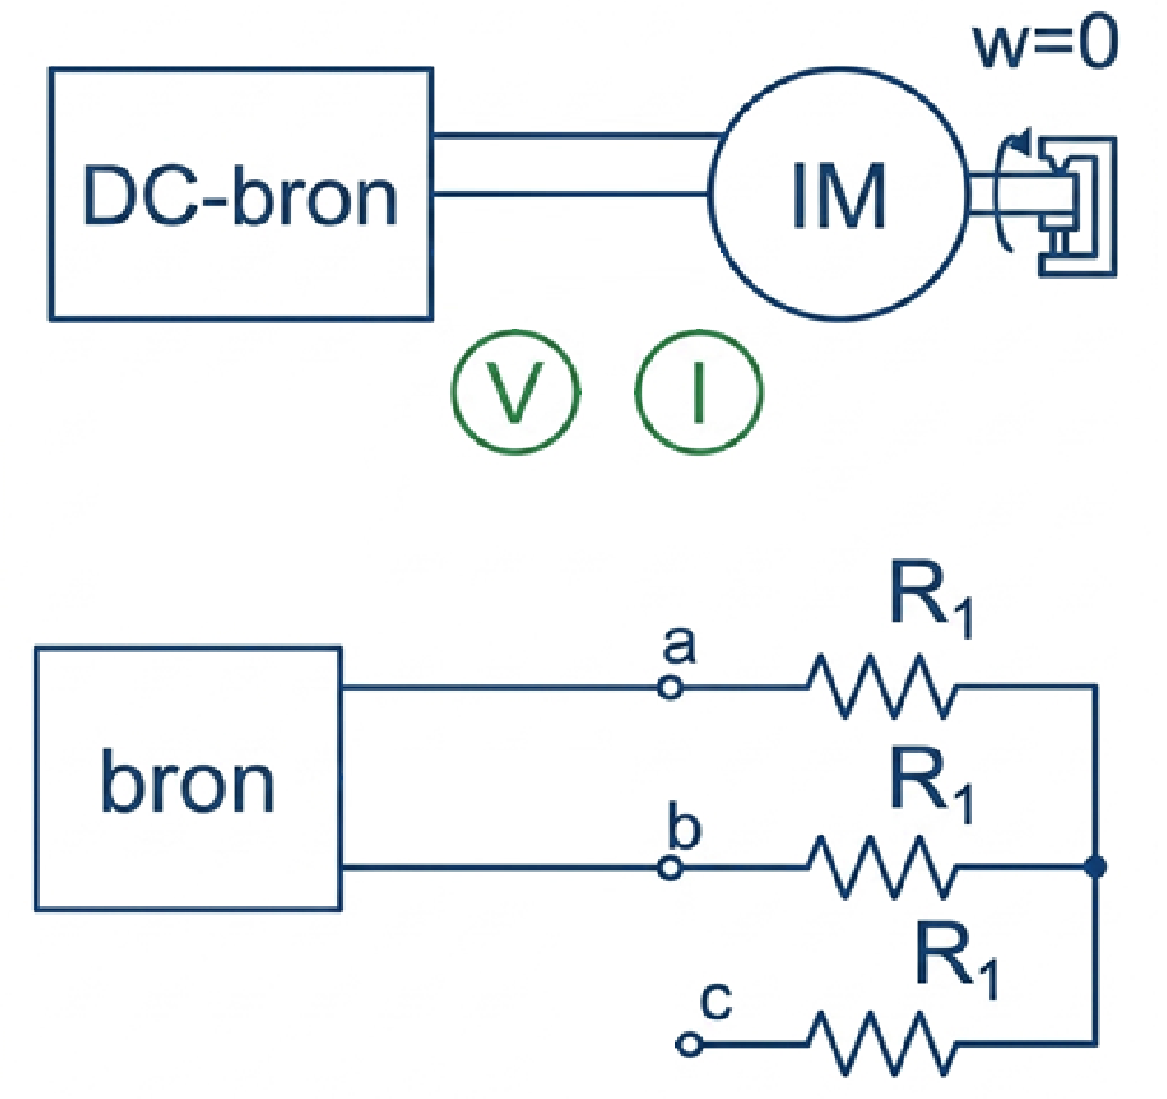
\includegraphics[width=0.4\textwidth]{assets/opstellingdcweerstandsmeting.png}
  \caption{Opstelling DC weerstandsmeting}
  \label{fig:opstellingdcweerstandsmeting.png}
 \end{figure}
We gaan hierdan dus een DC stroom door 2 $R_1$ weerstanden sturen, doordat het DC is gaan de spoelen geen effect hebben en kunnen we gewoon de weerstand meten zoals we zien in onderstaande schema:
\begin{figure}[H]
  \centering
  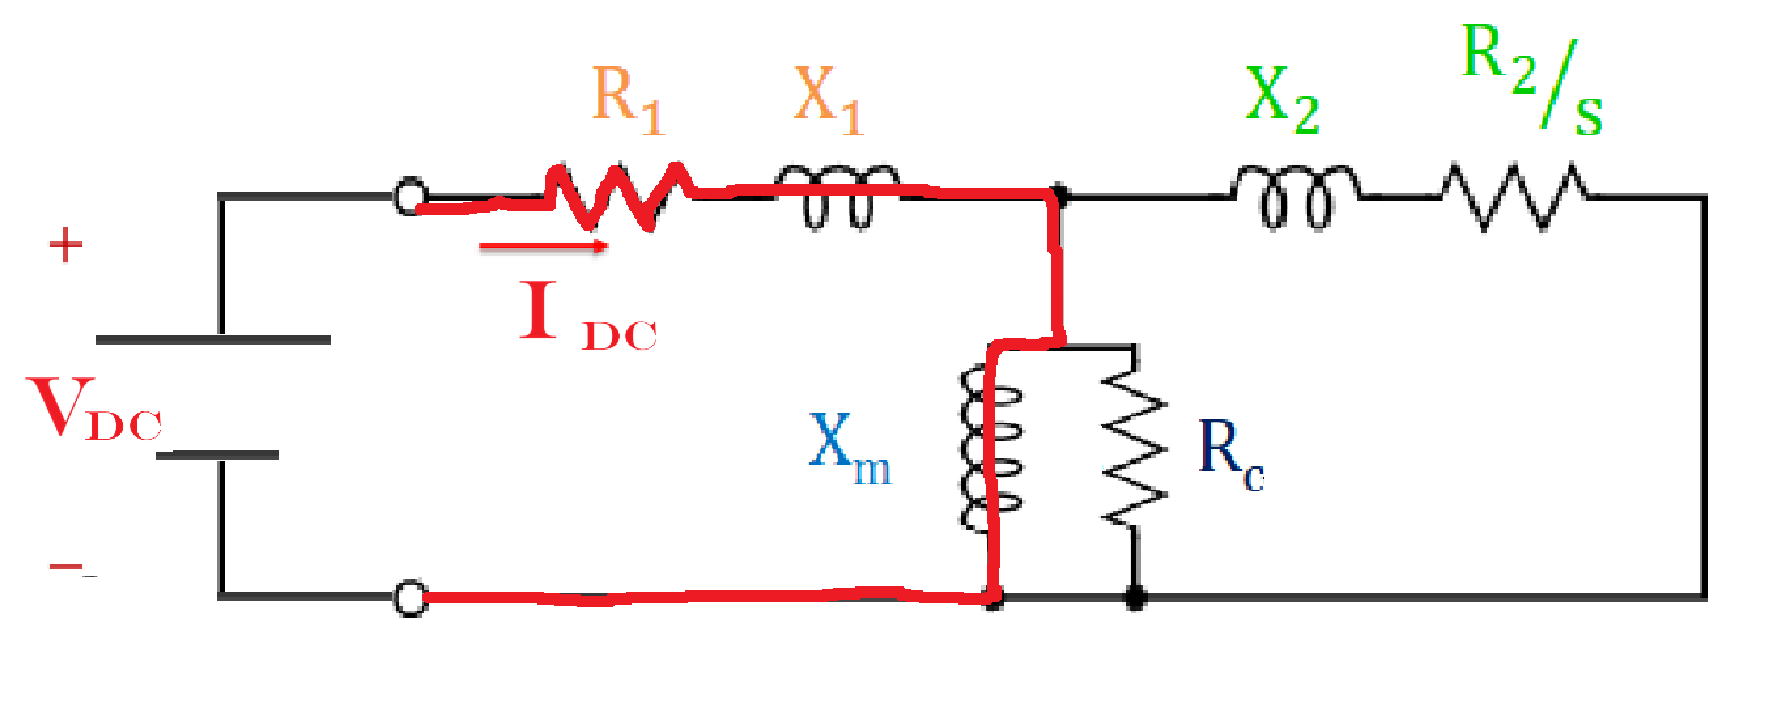
\includegraphics[width=0.8\textwidth]{assets/stroomverloopdcweerstandsmetong.png}
  \caption{DC stroom weerstandsmeting}
  \label{fig:stroomverloopdcweerstandsmetong.png}
 \end{figure}
Let dus wel op want hierboven is het een 1-fasig schema, ook is de onderste klem van de figuur hierboven eigelijk de neuter, in de 1ste figuur zagen we dat we door 2 $R_1$ weerstanden gingen dus de $R_1$ weerstand kan berekend worden met:
\begin{align*}
    R_1 = \frac{V_{DC}}{2 \cdot I_{DC}}
\end{align*}
Dit is een goede benadering van de weerstand, in het echt verschilt deze nog een beetje want bij AC heb je ook nog skin-effect. Zie ook dat je deze proef als laatste doet want eigelijk wil je deze weerstand meten op de steady-state temperatuur van de machine want normaal als hij draait warmt hij op en dan is de weerstand anders.
\subsubsection{Nullastproef}
Bij de nullastproef is het doel om de verliezen te meten (de wrijvings en ijzerverliezen). Hier laten we de motor op volle snelheid draaien ($n_s$) en we hangen er geen last aan ook dus $T = 0$, ook veronderstellen we geen mechanische verliezen, dit betekent dat $R'_{load}$ naar oneindig gaat (open keten). De nominale spanning sluiten we aan en we gaan dan de spanning, stroom en vermogen meten zoals we zien in de volgende opstelling:
\begin{figure}[H]
  \centering
  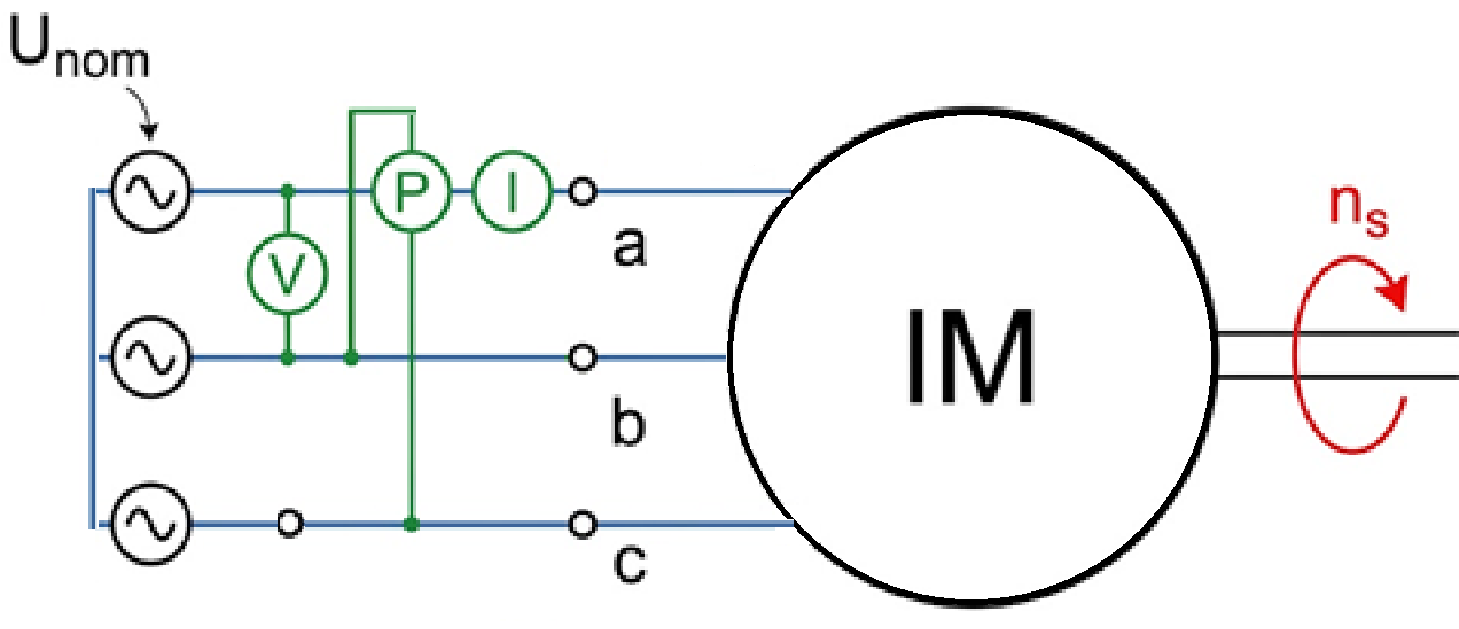
\includegraphics[width=0.6\textwidth]{assets/opstellingnullastproef.png}
  \caption{Opstelling nullastproef inductiemachine}
  \label{fig:opstellingnullastproef.png}
 \end{figure}
Doordat het op synchrone snelheid is gaat er dus ook geen spanning geïnduceerd worden en geen stroom vloeien (ook logisch als die weerstand oneindig is) dus het hele rotor gedeelte van het equivalent schema valt dus weg, oftewel zoals ik net eigelijk al zei, dit wordt een open keten. Het equivalent schema voor deze proef ziet er dan zo uit:
\begin{figure}[H]
  \centering
  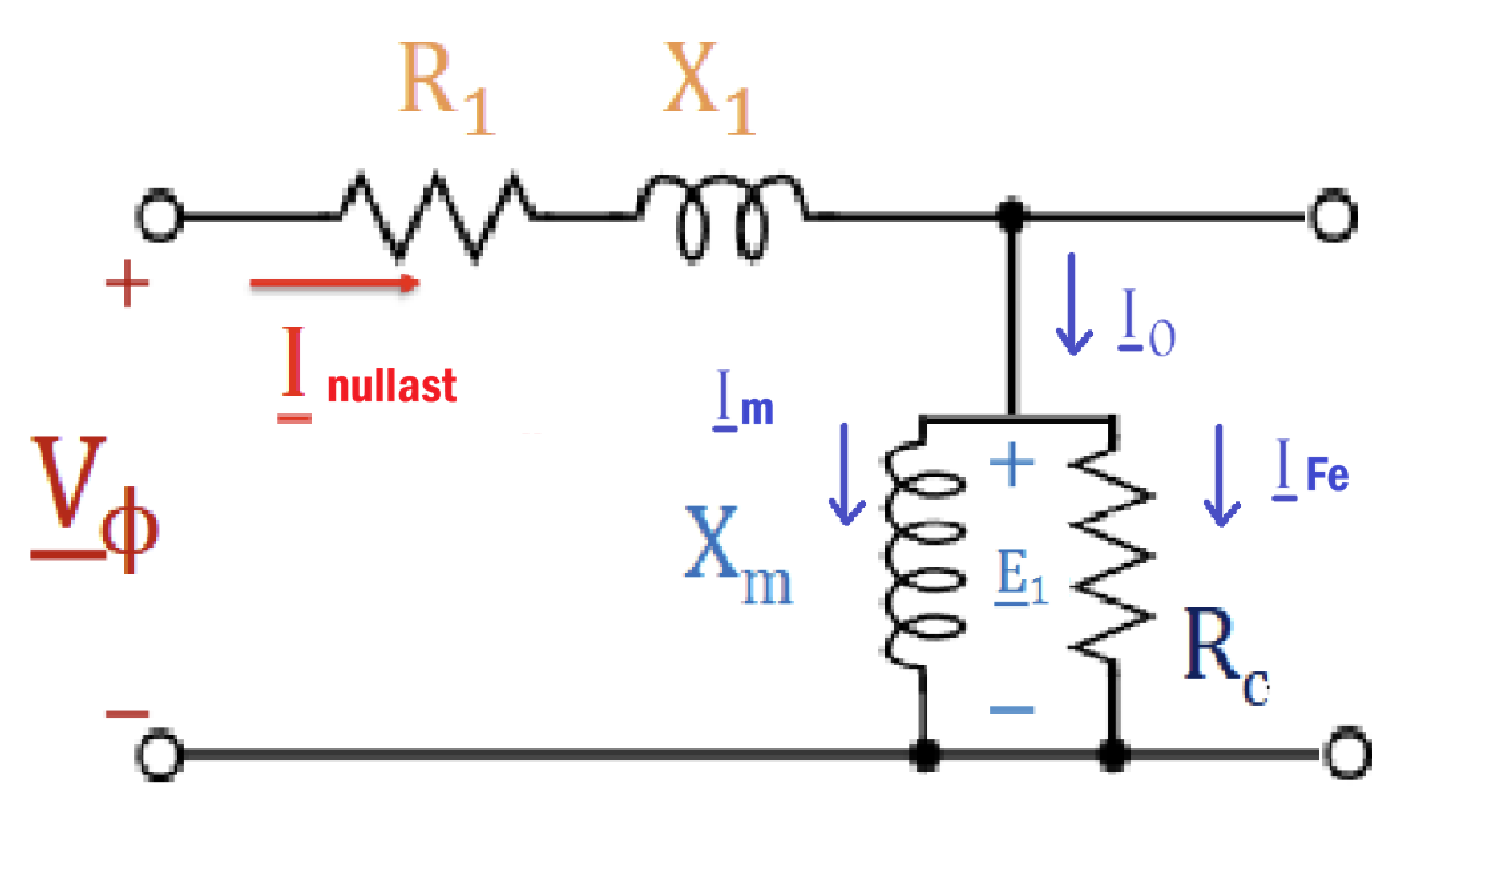
\includegraphics[width=0.6\textwidth]{assets/equivschemanullastproefIM.png}
  \caption{Equivalent schema nullastproef inductiemachine}
  \label{fig:equivschemanullastproefIM.png}
 \end{figure}
($I_{Nullast}$ is eigelijk exact hetzelfde als $I_0$ in dit equivalent schema)
\newline
\newline
Als we nu het vermogen meten als $P_{Nullast}$ dan is dit de som van de ijzerverliezen en de wrijvingsverliezen:
\begin{align*}
    P_{Nullast} = P_{R_1} + P_{R_{Fe}} = \underbrace{3 \cdot I_{Nullast}^2 \cdot R_1}_{\text{Kunnen we berekenen}} + 3 \cdot \frac{E_1^2}{R_{Fe}}
\end{align*}
Aangezien de spanningsval over $R_1$ en $X_1$ klein is tegenover $V_\phi$ kunnen we eigelijk de benadering maken dat $E_1 \approx V_\phi$ en dus kunnen we $R_{Fe}$ berekenen met:
\begin{align*}
    R_{Fe} = \frac{3 \cdot V_\phi^2}{P_{Nullast} - 3 \cdot I_{Nullast}^2 \cdot R_1}
\end{align*}
Met deze zelfde aanname ($R_{Fe}, X_m >> R_1, X_1$ en $E_1 \approx V_\phi$) kunnen we ook $X_1 + X_m$ berekenen met:
\begin{align*}
    X_1 + X_m = \frac{3 \cdot V_\phi^2}{Q_{Nullast}} = \frac{3 \cdot V_\phi^2}{\sqrt{S_{Nullast}^2 - P_{Nullast}^2}}
\end{align*}
Want $S_{Nullast} = \sqrt{3} \cdot V_L \cdot I_L = 3 \cdot V_\phi \cdot I_0$ en $Q_{Nullast} = \sqrt{S_{Nullast}^2 - P_{Nullast}^2}$.
\subsubsection{Blokkeerproef (Locked rotor test)}
Hier is het doel om $R_2$ en $X_1 + X_2$ te bepalen. We blokkeren hierbij de rotor (mechanisch) zodat $n = 0$ en dus $s = 1$. Daardoor geldt het volgende:
\begin{align*}
    R'_{load} = \frac{1-s}{s} \cdot R_2 = 0
\end{align*}
Dus die tak valt weg, we hebben gewoon de volgende parameters in serie want we gaan de parallele tak van $R_C$ en $X_m$ verwaarlozen want er zijn hier veel minder verliezen doordat we spanning gaan verlagen zodat de stroom niet te groot wordt (spanning van 0 regelen tot de nominale waarde van de stroom bereikt wordt). Er gaat dus weinig vermogen naar die magnetiseertak. Dus behouden we het volgende equivalent schema:
\begin{figure}[H]
  \centering
  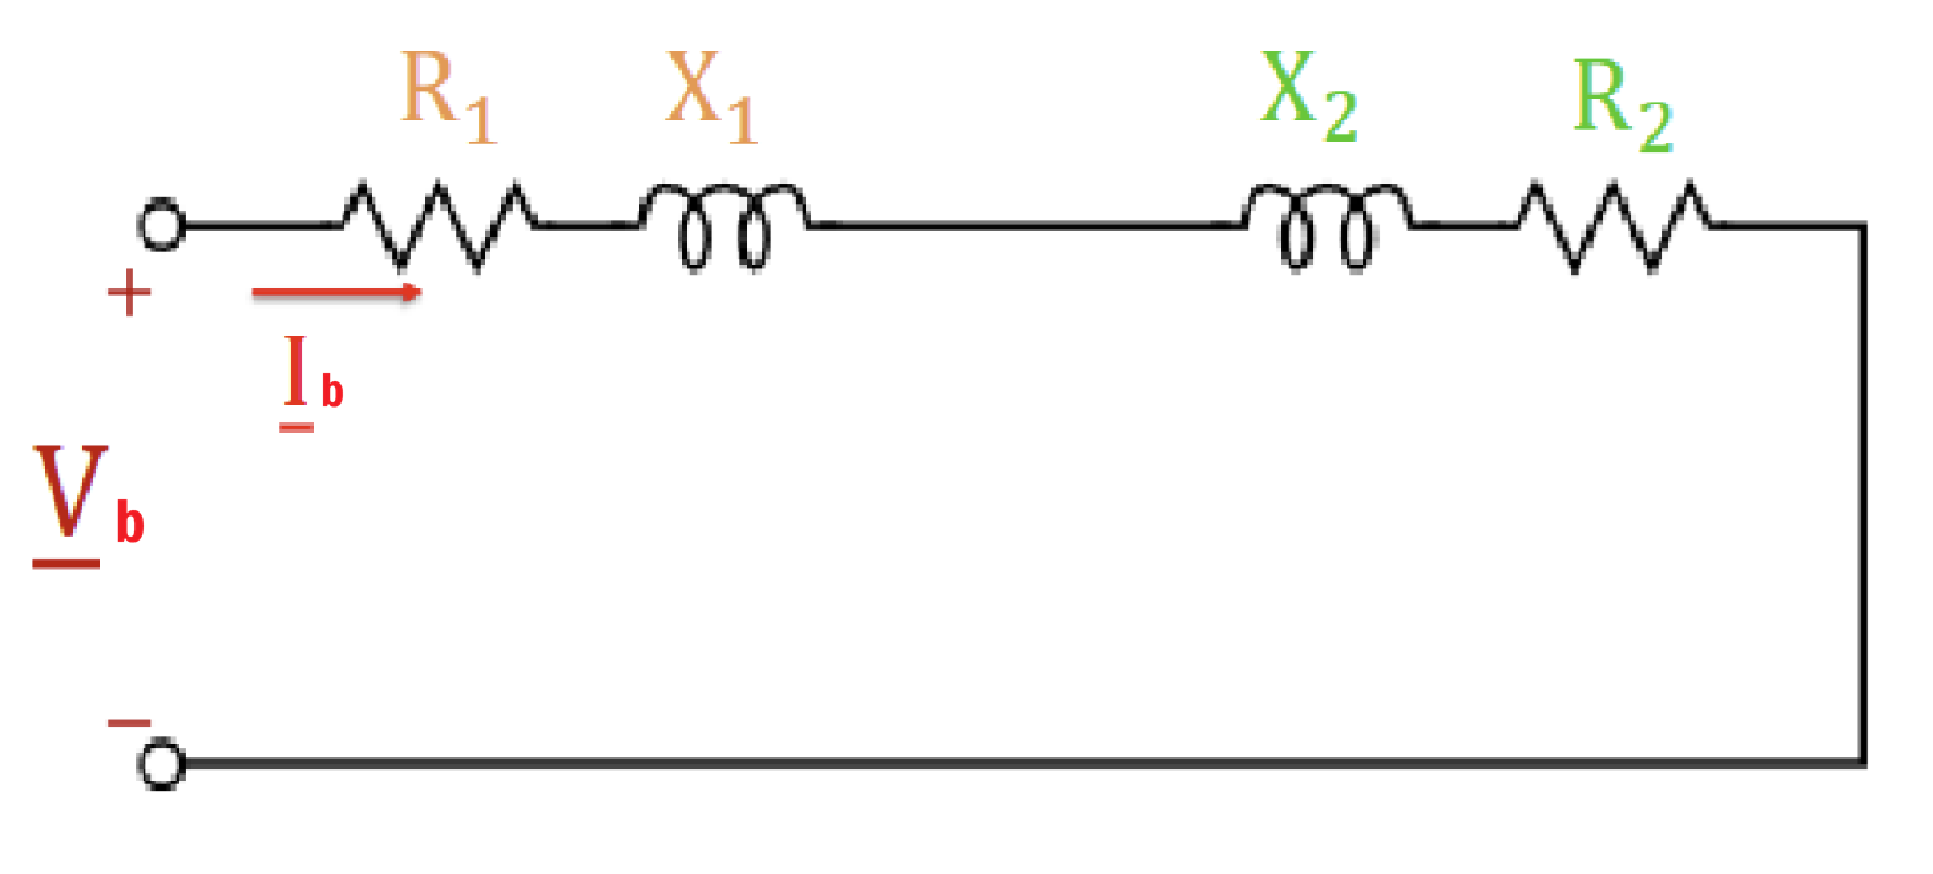
\includegraphics[width=0.6\textwidth]{assets/equivalentschemablokkeerproef.png}
  \caption{Equivalent schema blokkeerproef inductiemachine}
  \label{fig:equivalentschemablokkeerproef.png}
 \end{figure}
Als we nu het vermogen meten als $P_{Blokkeer}$ dan is dit de som van de stator en rotor verliezen:
\begin{align*}
    P_{Blokkeer} = P_{R_1} + P_{R_2} = \underbrace{3 \cdot I_{Blokkeer}^2 \cdot R_1}_{\text{Kunnen we berekenen}} + 3 \cdot I_{Blokkeer}^2 \cdot R_2
\end{align*}
De stroom weten we ook dus hiermee kunnen we gewoon $R_2$ berekenen. Je gaat hier zien dat deze inderdaad verschilt van $R_1$ zoals we eerder zeiden.
\newline
\newline
Met de blokkeer spanning kunnen we totale impedantie berekenen:
\begin{align*}
    Z_{Blokkeer} = \frac{V_{Blokkeer}}{I_{Blokkeer}} = \sqrt{(R_1 + R_2)^2 + (X_1 + X_2)^2}
\end{align*}
Hiermee kunnen we dus $X_1 + X_2$ berekenen. Oftewel $X_{tot}$, maar we gaan dit $X'_{tot}$ noemen want dit is eigelijk niet de 'echte' $X_{tot}$. Deze is namelijk op een frequentie van 15Hz bepaald, niet 60Hz. Die 15Hz komt van het feit dat normaal de stator 60Hz en de rotor 1Hz ofzo heeft, die 15Hz dat we nemen is hier een compromis omdat het hier in serie is allemaal. 60Hz zorgt voor teveel skin-effecti in de rotorstaven, 15Hz is een mooie benadering van het echte lekgedrag. Omzetten naar het echte kan wel aan de hand van $X = \omega L$ want L is frequentie onafhankelijk:
\begin{align*}
 X'_{tot} = \omega_{15} \cdot L_{lek, S+R} = 2 \cdot \pi \cdot 15 Hz \cdot L_{lek, S+R} \\
 X_{tot} = X_{lek S+R @60 Hz} = 2 \cdot \pi \cdot 60 Hz \cdot L_{lek, S+R} 
\end{align*}
Dus eigelijk geldt:
\begin{align*}
    X_{tot} = X'_{tot} \cdot \frac{60}{15} = 4 \cdot X'_{tot}
\end{align*}
Om te splitsen naar $X_1$ en $X_2$ gebruiken we standaardverhoudingen genaamd NEMA verhoudingen, deze bepalen dus de verhouding tussen $X_1$ en $X_2$. Deze kunnen afgelezen worden uit een tabel, maar als er niks wordt gegeven of gezegd mogen we een 50/50 verhouding gebruiken:
\begin{figure}[H]
  \centering
  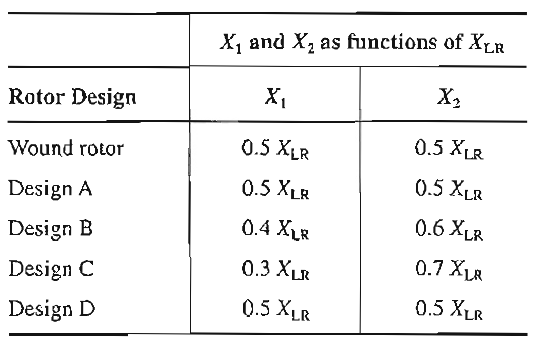
\includegraphics[width=0.4\textwidth]{assets/nemaverhoudingen.png}
  \caption{NEMA verhoudingen voor het splitsen van $X_1$ en $X_2$}
  \label{fig:nemaverhoudingen.png}
 \end{figure}
\section{Koppel-toerentalkarakteristiek}
Dan gaan we nu eens meer uitgebreid kijken naar de koppel-toerentalkarakteristiek van de inductiemachine. We hebben al eerder gezien dat deze er ongeveer zo uitziet:
\begin{figure}[H]
  \centering
  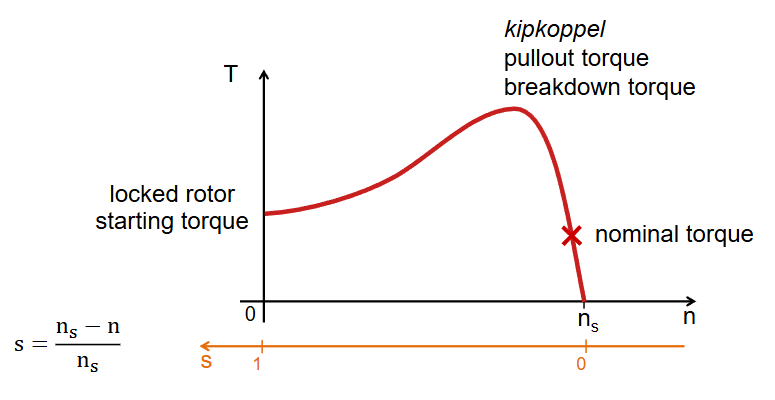
\includegraphics[width=0.6\textwidth]{assets/TNinductiemachine.png}
  \caption{Koppel-toerentalkarakteristiek van de inductiemachine}
  \label{fig:TNinductiemachine.png}
 \end{figure}
Het gebied dat voor die piek van het \textbf{kipkoppel} (maximale koppel dat de machine kan leveren) is een gebied waar we normaal niet werken. (Dit zien we later nog waarom niet). Dit is het \textit{onstabiel gebied}, hier hebben we ons \textbf{startkoppel}. Van die piek (kipkoppel) tot dat \textit{'nominal torque'} punt (oftewel ons stabiel punt) hebben we ons \textit{stabiel gebied}, hier kunnen we kortstandig werken want het is eigelijk overbelasting. Ideaal werken we rond dat stabiel werkingspunt op het \textbf{nominaal koppel} $T_{nom}$ het gebied hierna willen we niet werken omdat dit een slechte arbeidsfactor heeft. Deze machine kan zoals we zien rechtstreeks van het net starten.
\newline
\newline
Om die T-n karakteristiek te berekenen hebben we de formule nodig van het koppel van de inductiemachine. We gaan dit doen aan de hand van het conventieel vermogen (we gaan dus van geen verliezen in de as uit). We hebben deze formule eerder al gezien eigelijk, nu gaan we tonen vanwaar die komt en hoe het dus de T-n karakteristiek bepaald. We weten dus dat dit $P_{conv}$ is:
\begin{align*}
    P_{conv} = T_{ind} \cdot \omega
\end{align*}
In functie van de synchrone snelheid is dit:
\begin{align*}
    P_{conv} = T_{ind} \cdot \omega_s \cdot (1-s)
\end{align*}
Ook weten we dat $P_{conv} = P_S - P_{Cu,r}$ (Zie eerder het vermogen balans) dus:
\begin{align*}
    P_{conv} = P_S - P_{Cu,r} = 3 \cdot I_2^2 \cdot \frac{R_2}{s} - 3 \cdot I_2^2 \cdot R_2 = 3 \cdot I_2^2 \cdot R_2 \left(\frac{1-s}{s}\right)
\end{align*}
Hieruit kunnen we dus het koppel berekenen:
\begin{align*}
    T_{ind} = \frac{P_{conv}}{\omega_s \cdot (1-s)} = \frac{3 \cdot I_2^2 \cdot R_2 \left(\frac{1-s}{s}\right)}{\omega_s \cdot (1-s)} = \frac{3 \cdot I_2^2 \cdot R_2}{\omega_s \cdot s}
\end{align*}   
Dit is dus het geïnduceerde koppel van de inductiemachine. De proff specifieert ook dat het belangrijk is om te weten dat de stroom $I_2$ (en ook $I_1$) in functie zijn van de slip $s$ en de spanning $V_\phi$ verandert, dus dit is niet een constante! Voor deze stroom is een complexe formule, die we niet moeten kennen, maar ik zet ze hier toch, want deze wordt wel gebruikt om de uiteindelijke formule van het koppel te berekenen:
\begin{align*}
    I_1 = V_\phi \cdot \frac{\frac{R_2}{s} + j(X_1 + X_2)}{\frac{R_1 R_2}{s} - X_m \cdot (X_1 + X_2) - X_1 X_2 + j(R_1 X_m + R_1 X_2 + \frac{R_2 X_m}{s} + \frac{R_2 X_1}{s})}
\end{align*}
Het koppel hiermee wordt dan:
\begin{align*}
    T_{ind} = \frac{3 \cdot V_{TH}^2 \cdot \frac{R_2}{s}}{\omega_s \cdot [\left(R_{TH} + \frac{R_2}{s}\right)^2 + (X_{TH} + X_2)^2]}
\end{align*}
Met:
\begin{align*}
    V_{TH} = V_\phi \cdot \frac{X_m}{\sqrt{R_1^2 + (X_1 + X_m)^2}} \\
    R_{TH} = \frac{R_1 \cdot X_m^2}{R_1^2 + (X_1 + X_m)^2} \\
    X_{TH} \approx \frac{X_1 \cdot X_m}{X_1 + X_m}
\end{align*}
In de formule van het koppel gaan we nog een paar aanpassingen doen om dit simpeler te maken, we gaan namelijk de hele formule vermenigvuldigen met $\frac{s^2}{s^2}$ en dan de term $R_{TH} \cdot s$ dat je dan krijgt in de noemer verwaarlozen, zo krijgen we de volgende formule:
\begin{align*}
    \boxed{T_{ind} = \frac{3 \cdot V_{TH}^2 \cdot R_2 \cdot s}{\omega_s \cdot [ {\color{red}R_2^2 + } {\color{blue}s^2 \cdot (X_{TH} + X_2)^2}]}}
\end{align*}
Het is dus deze formule dat gebruikt wordt om de T-n karakteristiek te berekenen. Bij grote slip wordt de rode term verwaarloosd en het linkse gedeelte van de T-n karakteristiek van de volgende figuur bepaald (dit is eigelijk hyperbolisch want de formule krijgt de vorm van $k = \frac{1}{s}$) en bij kleine slip wordt de blauwe term verwaarloosd en het rechtse gedeelte van de T-n karakteristiek bepaald. Het maximum van deze kromme is het kipkoppel, deze staat hier niet op maar kan wel gevonden worden door de 1ste afgeleiden naar de slip te nemen en deze gelijk te stellen aan 0. (Dit geeft de kipslip)
\begin{figure}[H]
  \centering
  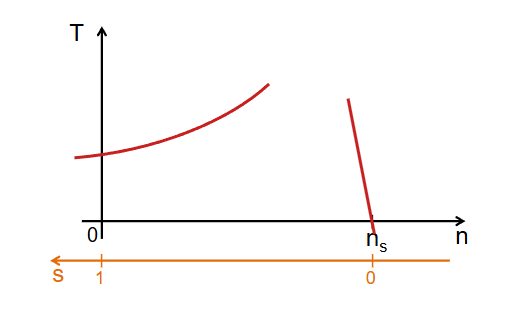
\includegraphics[width=0.5\textwidth]{assets/TNkarakteristiekzonderkippiek.png}
  \caption{T-n karakteristiek van de inductiemachine zonder het kipkoppel aangeduid}
  \label{fig:TNkarakteristiekzonderkippiek.png}
 \end{figure}
Formules voor de kipslip en het kipkoppel zijn:
\begin{align*}
    s_{kip} = \frac{R_2}{\sqrt{R_{TH}^2 + (X_{TH} + X_2)^2}} \\
    T_{kip} = \frac{3}{\omega_s} \cdot \frac{V_{TH}^2}{2[R_{TH} + \sqrt{R_{TH}^2 + (X_{TH} + X_2)^2}]}
\end{align*}
We zien dus dat de kipslip afhankelijk is van de rotorweerstand $R_2$ en niet van de spanning! En het geïnduceerd koppel ook maar deze is wel ook afhankelijk van de spanning ($T_{ind} \propto V_{TH}^2$) (en $V_\phi \approx V_{TH}$). Dit is belangrijk want dit betekent dat we het koppel kunnen regelen door de spanning te regelen, dit is eigelijk ook wel nadelig bij bvb. spanningsdips. 
\subsection{Variaties in de T-n karakteristiek}
Nu gaan we kijken naar een paar factoren die invloed kunnen hebben op de koppel-toerentalkarakteristiek van de inductiemachine.
\subsubsection{Statorspanning}
Dus we weten nu dat het koppel afhankelijk is van de spanning in het kwadraat ($T \approx V_\phi^2$). Bij een spanningsdip kan dit dus problematisch zijn, door dit kwadraat gaat het koppel rap sterk dalen dan en afhankelijk van welke toepassing je de inductiemachine gebruikt kan dit problematisch zijn. We zullen is aan de hand van volgende grafiek bespreken wat er precies gebeurt bij zo een spanningsdip:
\begin{figure}[H]
  \centering
  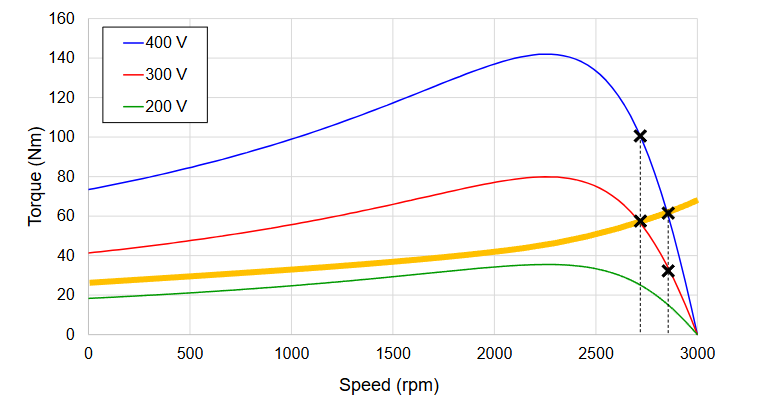
\includegraphics[width=0.6\textwidth]{assets/TNkarakteristiekverschillendespanningenenlastkarakteristiek.png}
  \caption{T-n karakteristiek bij verschillende spanningen + de lastkarakteristiek}
  \label{fig:TNkarakteristiekverschillendespanningenenlastkarakteristiek.png}
 \end{figure}
Stel we hebben 400V en een spanningsdip brengt ons naar 300V zoals in bovenstaande figuur, dan zien we dat ons stabiel werkingspunt eerst naar beneden zakt want van zodra de spanningsdip gebeurt is ons motor nog op dezelfde snelheid, daarna zien we echter dat onze snelheid zal moeten vertragen tot een nieuw evenwicht voor onze last. Hier bij die 300V is dit nog niet zo erg zien we want zodra de spanningsdip over is kunnen we terug naar ons vorig evenwicht gaan. Het is pas een probleem als we niet genoeg koppel meer hebben om de last te kunnen blijven aandrijven zoals bevoorbeeld als onze spanningsdip tot die 200V daar gaat, dit is onder die gele last karakteristiek. Dus de spanningsdip is dan zo laag dat de motor kan uitvallen.
\subsubsection{Rotorweerstand}
We zagen dus eerder dat ons koppel ook afhankelijk is van de rotorweerstand $R_2$. Dit kan handig zijn soms, want als we deze weerstand groter kunnen maken kunnen we een groter startkoppel hebben en vooral dan ook een \textbf{lagere startstroom}. Terwijl ons maximaal koppel hetzelfde blijft (wel meer slip dus meer slipverliezen). Dit kunnen we toepassen met 'rotorweerstanden' zoals in de volgende figuren:
\begin{figure}[H]
  \centering
  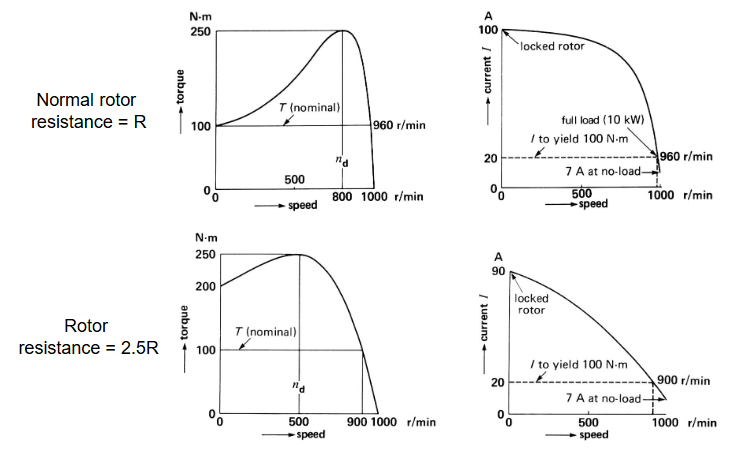
\includegraphics[width=0.7\textwidth]{assets/rotorweerstand1.png}
  \caption{Rotorweerstanden R en 2.5R}
  \label{fig:rotorweerstand1.png}
 \end{figure}
\begin{figure}[H]
  \centering
  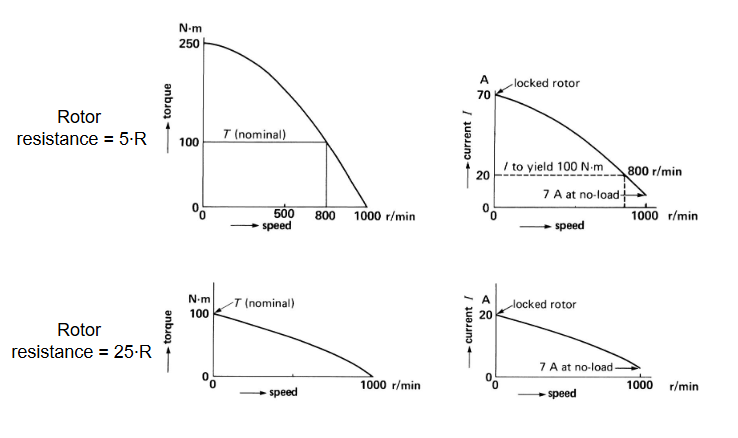
\includegraphics[width=0.7\textwidth]{assets/rotorweerstand2.png}
  \caption{Rotorweerstanden 5R en 25R}
  \label{fig:rotorweerstand2.png}
 \end{figure}
We zien dus dat bij grotere rotorweerstanden het startkoppel groter wordt en de startstroom kleiner. Maar wat we ook zien is dat de snelheid voor het nominaal koppel gaat dalen, soms zelfs zo hard dat dit niet meer interessant is als je de motor op die snelheid continu wilt laten werken. Eigelijk willen we liefst bij opstart een grotere rotorweerstand om grotere lasten te kunnen overwinnen maar voor ons nominaal koppel willen we een kleinere rotorweerstand. Om dit te doen maken we gebruik van een \textbf{gewikkelde rotor} zodat we de wikkelingen van de rotor via de sleepringen dan langs buiten kunnen aansluiten aan weerstanden (of kortsluiten). Ook kunnen zo die weerstanden langs buiten makkelijker gekoeld worden.
\begin{figure}[H]
  \centering
  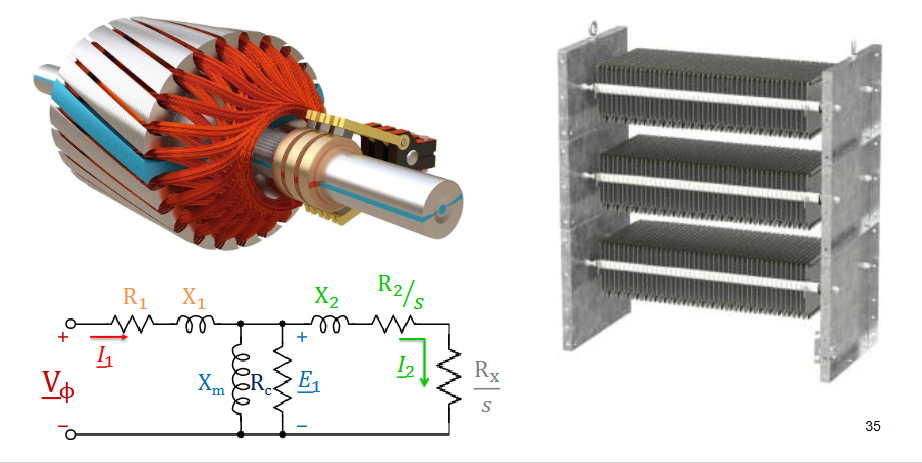
\includegraphics[width=0.6\textwidth]{assets/gewikkelderotormetweerstandenencircuitenkoelsysteem.png}
  \caption{Gewikkelde rotor met weerstanden en circuite en koelsysteem}
  \label{fig:gewikkelderotormetweerstandenencircuitenkoelsysteem.png}
 \end{figure}
Wat we ook kunnen doen is een ander soort rotor gebruiken. De NEMA-klassen classificeren rotors (motoren eigelijk) op basis van hun kopel, je kan hier dus ook naar kijken en kiezen. Je kan bevoorbeeld een dubbele kooi rotor hebben. Deze zorgen voor veel weerstand zodat je een groot startkoppel hebt en hebben eigelijk ook een soort van adaptieve weerstand (ze zijn groter bij start), op de volgende figuur zie je karakteristieken van een paar van die verschillende klasse motoren, sommige hebben een \textbf{zadelpunt}:
\begin{figure}[H]
  \centering
  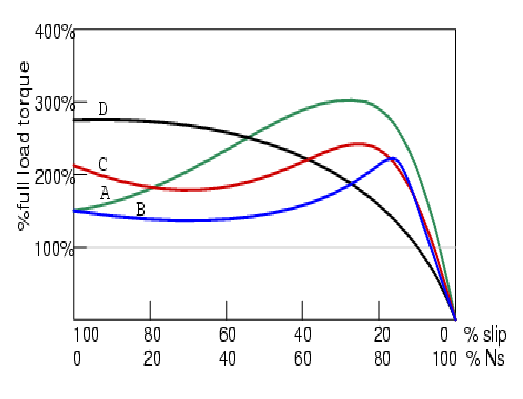
\includegraphics[width=0.5\textwidth]{assets/karakteristiekenmotorsnema.png}
  \caption{Karakteristieken van NEMA-klassen motoren}
  \label{fig:karakteristiekenmotorsnema.png}
 \end{figure}
Een \textbf{dubbele kooi rotor} heeft dus 2 kooien, een binnenste en een buitenste. De buitenste kooi heeft een hoge weerstand en een lage inductantie, deze zorgt voor een groot startkoppel. De binnenste kooi heeft een lage weerstand en een hoge inductantie, deze zorgt voor een hoog nominaal koppel. Het nadeel van deze motoren is dat ze duurder zijn dan de standaard motoren.
\begin{figure}[H]
  \centering
  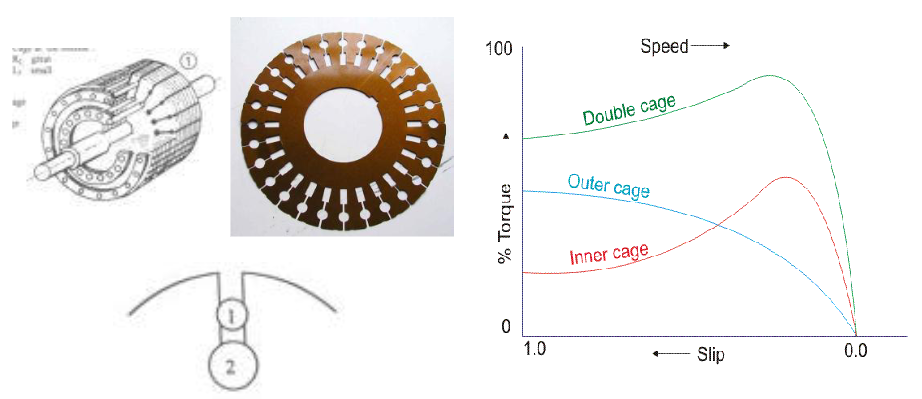
\includegraphics[width=0.8\textwidth]{assets/dubbelekooirotor.png}
  \caption{Dubbele kooi rotor}
  \label{fig:dubbelekooirotor.png}
 \end{figure}
\subsubsection{Uitgebreide T-n karakteristiek}
De formule die we eerder hadden afgeleid hadden we toen gebruikt voor onze T-n karakteristiek, maar eigelijk werkte die formule even goed om die karakteristiek uit te breiden zoals in de volgende figuur:
\begin{figure}[H]
  \centering
  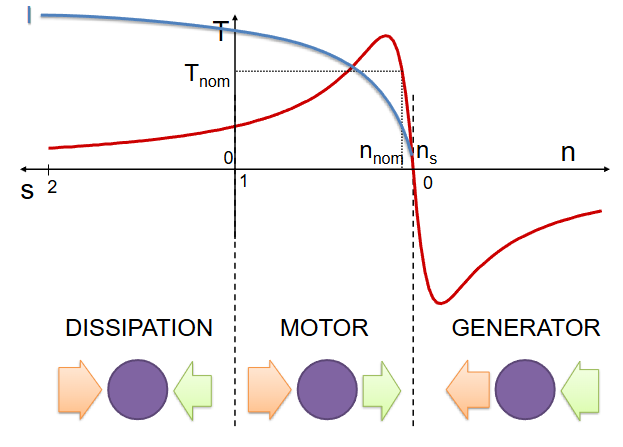
\includegraphics[width=0.5\textwidth]{assets/uitgebreideTNkarakteristiekIM.png}
  \caption{Uitgebreide T-n karakteristiek}
  \label{fig:uitgebreideTNkarakteristiekIM.png}
 \end{figure}
Deze curve komt dus ook van die formule en is even correct, we zien hier namelijk ook de generatorwerking gedeelte van de curve, hier hebben we nog steeds een positieve snelheid maar nu bij een negatief koppel en negatieve slip. Wat we ook nog kunnen hebben is \textbf{dissipatie} hier sturen we eigelijk 2 vermogens de machine in zoals je ziet bij die pijlen (de oranje pijl is het elektrisch vermogen, de groene pijl is het mechanisch vermogen). De slip is hier ook groter dan 1, alles wordt hier omgezet in warmte. Op deze figuur zien we ook de curve van de strool en is het duidelijk dat we grote startstromen hebben bij een grote slip, dit is dus ook de reden waarom we niet in dat onstabiel gebied willen werken.
\subsubsection{4 kwadranten werking}
We kunnen deze curve eigelijk opdelen in 4 kwadranten als volgt:
\begin{figure}[H]
  \centering
  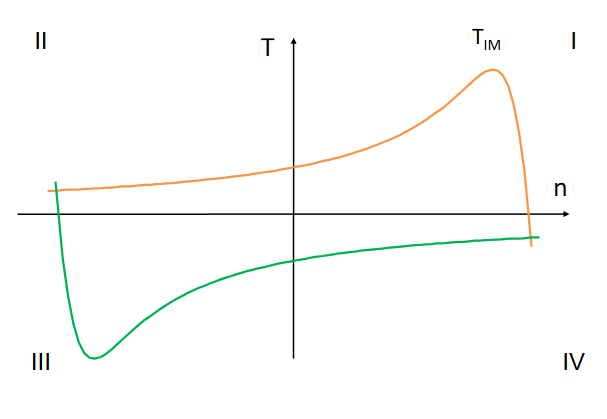
\includegraphics[width=0.6\textwidth]{assets/4kwadrantenwerking.png}
  \caption{T-n curve 4 kwadranten}
  \label{fig:4kwadrantenwerking.png}
 \end{figure}
Dit is gewoon hetzelfde als we eerder zagen maar 2 keer getekend, de oranje curve is de nomrale T-n karakteristiek van de motor met ook de negatieve n en negatieve T nog een beetje getoond. De groene curve is exact hetzelfde maar $180^\circ$ gedraaid rond de oorsprong, dit bekrijg je door 2 van de 3 fasen te wisselen (draaiveld omkeren), dit is dus het spiegelbeeld. De T en n-as verdelen zo het vlak in 4 kwadranten (I,II,III,IV). De figuur toont dus eigelijk (als je beide curves samen bekijkt) dat de as van de machine in elke combinatie van draairichting en koppelrichting terecht kan komen (de 4 kwadranten). Om in het 3de kwadrant te komen moet je dus gewoon 2 van de 3 fases wisselen. Daar waar die 2 curves snijden in het 4de kwadrant, dus vanaf een bepaalde snelheid, kan je in generator werking zitten. (Anders is de rest van dat kwadrant, en dus ook kwadrant 2, dissipatie)
\subsubsection{Ongebalanceerde voeding}
Een onbalans van het net kan ook invloed op het koppel hebben. Eerder gingen we er altijd vanuit dat ons net in balans was (3 fases met zelfde amplitude en verschuiving), bij onbalans op het net is dit dus niet het geval. In vorige cursussen zagen we dat onbalans opgesplitst kan worden in 3 componenten: de directe component, de inverse component en de homopolaire component. Zoals we zien in volgende figuur:
\begin{figure}[H]
  \centering
  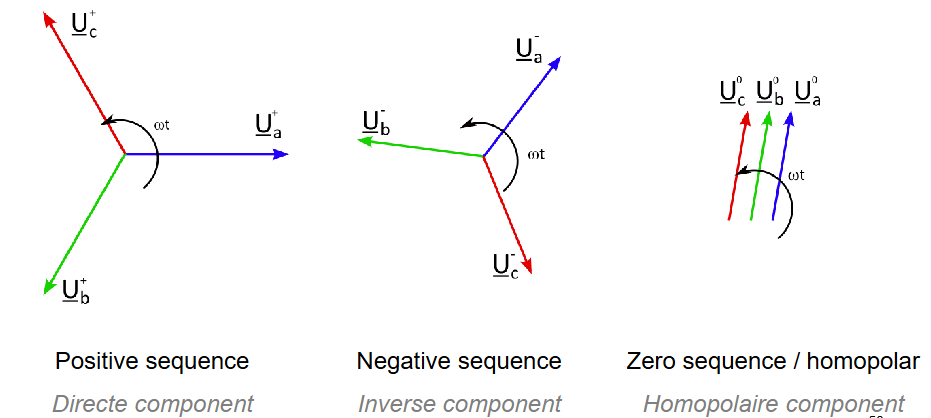
\includegraphics[width=0.7\textwidth]{assets/onbalanscomponenten.png}
  \caption{Directe, inverse en homopolaire componenten}
  \label{fig:onbalanscomponenten.png}
 \end{figure}
\begin{figure}[H]
  \centering
  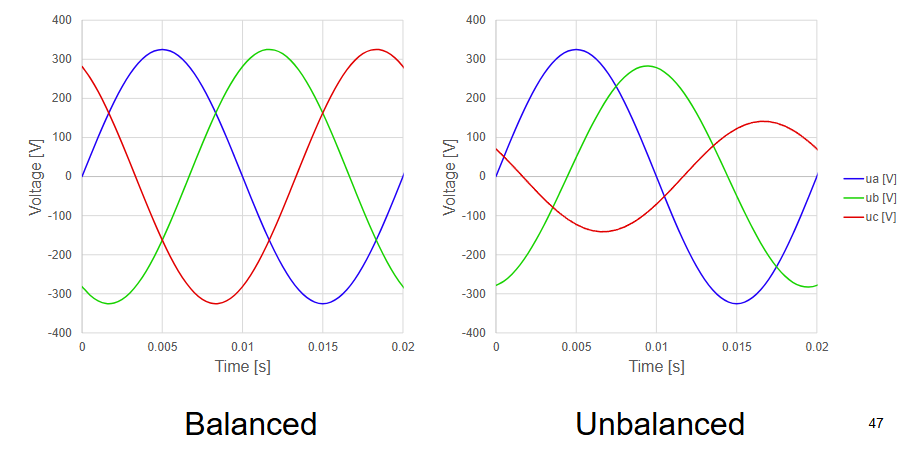
\includegraphics[width=0.6\textwidth]{assets/balancedenunbalancednet.png}
  \caption{Gebalanceerde en ongebalanceerde voeding}
  \label{fig:balancedenunbalancednet.png}
 \end{figure}
De directe component loopt zoals normaal en is ook meestal de grootste, de inverse component loopt in tegengestelde richting en is meestal kleiner, de homopolaire component heeft alle vectoren op één lijn liggen, hier is geen faseverschuiving tussen. De directe maakt een draaiveld in de ene richting terwijl de indirecte die in de andere richting maakt (de homopolaire maakt dus GEEN draaiveld), hierdoor gaan we een ellipsvormig draaiveld krijgen als resulterende van al deze componenten.
\begin{figure}[H]
  \centering
  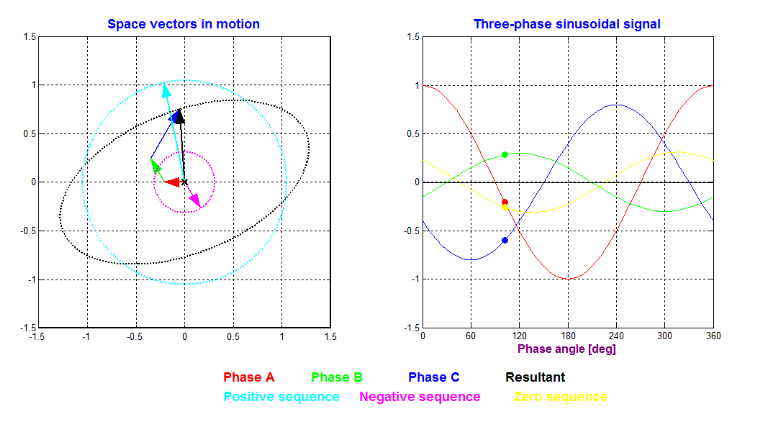
\includegraphics[width=0.6\textwidth]{assets/elliptischdraaiveld.png}
  \caption{Elliptisch draaiveld}
  \label{fig:elliptischdraaiveld.png}
 \end{figure}
Wat is nu dat effect van het elliptisch draaiveld op de T-n karakteristiek? Bekijk deze figuur, het is eigelijk de 4 kwadrant operatie:
\begin{figure}[H]
  \centering
  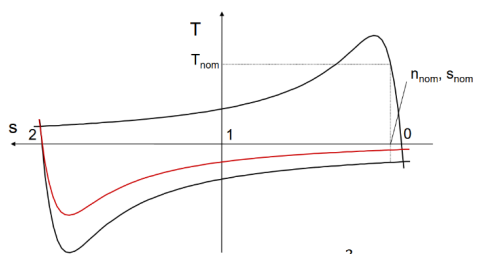
\includegraphics[width=0.6\textwidth]{assets/4kwadrantoperatiedirectenondirectecomponent.png}
  \caption{4 kwadrant operatie met directe en inverse component}
  \label{fig:4kwadrantoperatiedirectenondirectecomponent.png}
 \end{figure}
Die bovenste T-n karakteristiek is de normale karakteristiek, deze wordt gemaakt door de directe component. De onderste gespiegelde dan door de inverse component. Doordat de 2 koppels een andere amplitude kunnen hebben moeten deze dus ook geschaald worden als we het totale koppel willen bepalen, dit wordt dan gedaan met de volgende formule:
\begin{align*}
 T(s) = T_{+}(s) \cdot |{\frac{V_{+}}{V_{\phi}}}|^2 + T_{-}(s) \cdot |{\frac{V_{-}}{V_{\phi}}}|^2
\end{align*}
Want het koppel heeft een kwadratisch verband met de spanning. We willen zo weinig mogelijk van de inverse component want zoals we ziet zit die in dissipatie, dus dit brengt alleen extra hitte met zich mee. En dus ook zien we dat dit eigelijk een negatieve koppel is en zich dus aftrekt van het koppel van de directe component. Een onbalans kan dus het koppel licht doen verlagen maar zorgt wel voor veel extra opwarming.
\begin{figure}[H]
  \centering
  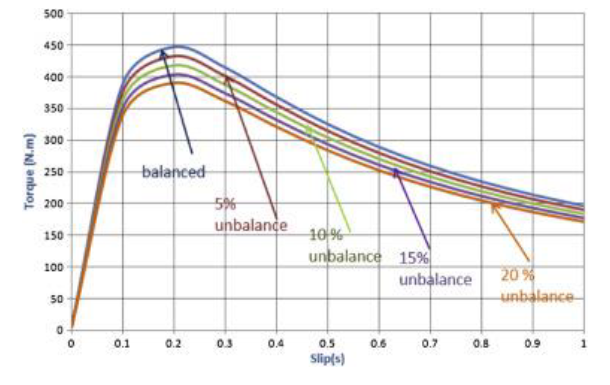
\includegraphics[width=0.6\textwidth]{assets/weergavekoppelverliesdooronbalans.png}
  \caption{Weergave koppelverlies door onbalans}
  \label{fig:weergavekoppelverliesdooronbalans.png}
 \end{figure}
Hierboven zie je dus hoeveel koppel je verliest met hoeveel percentage onbalans, niet super veel dus, niet problematisch. In de figuur hieronder zie je de temperatuurinvloed door onbalans, dit is duidelijk wel problematisch want dit doet de levensduur zakken. Je ziet dat een onbalans van slechts 3.5\% al voor een temperatuurverschil van 25\% kan zorgen.
\begin{figure}[H]
  \centering
  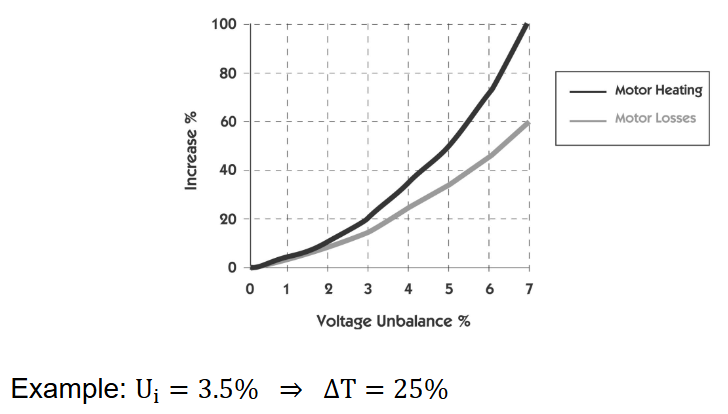
\includegraphics[width=0.5\textwidth]{assets/tempeffectonbalans.png}
  \caption{Temperatuur-effect van onbalans}
  \label{fig:tempeffectonbalans.png}
 \end{figure}
Wat is nu het effect van die homopolaire component? De homopolaire component is eigelijk 3 keer hetzelfde, het is dus eigelijk een 1-fasige wisselspanning en dit kan ook een koppel genereren, alleen kan het niet zelf starten:
\begin{figure}[H]
  \centering
  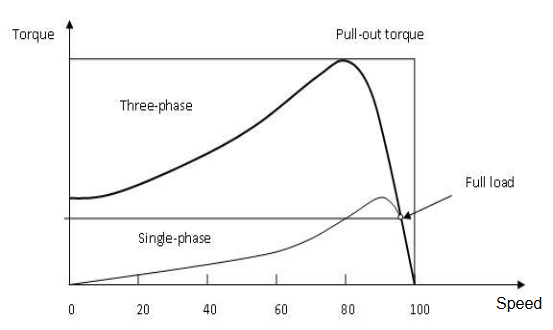
\includegraphics[width=0.6\textwidth]{assets/Tn3fasigen1fasig.png}
  \caption{Weergave koppel door homopolaire component}
  \label{fig:Tn3fasigen1fasig.png}
 \end{figure}
Maar eigelijk gedraagt zich dit als 3 enkelfasige motors waardoor we 3 keer zoveel polen hebben en dus een veel vroegere synchrone snelheid dan de directe en inverse component. Dit maakt dat we al rap in generatorwerking gaan zitten, wat een nefatieve invloed heeft, zoals we zien in volgende figuur:
\begin{figure}[H]
  \centering
  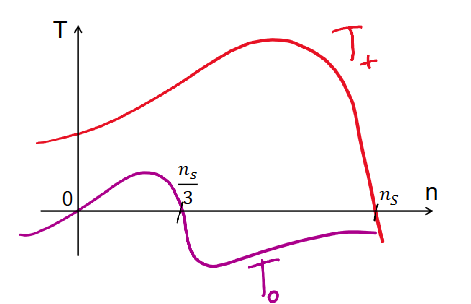
\includegraphics[width=0.5\textwidth]{assets/TNdirecteenhomopolairecomponent.png}
  \caption{T-n karakteristiek van de directe en homopolaire component}
  \label{fig:TNdirecteenhomopolairecomponent.png}
 \end{figure}
De echte formule voor $T(s)$ met de homopolaire component wordt dan:
\begin{align*}
 \boxed{T(s) = T_{+}(s) \cdot |{\frac{V_{+}}{V_{\phi}}}|^2 + T_{-}(s) \cdot |{\frac{V_{-}}{V_{\phi}}}|^2 + T_{0}(s) \cdot |{\frac{V_{0}}{V_l / 3}}|^2}
\end{align*}
Echter is die homopolaire component geen probleem want je kan die makkelijk wegwerken/niet laten mee tellen door je sterpunt zwevend te laten (geen Neutraal (N) aan te sluiten) in je sterschakeling, of door sowieso een driehoekschakeling te gebruiken (die heeft toch geen sterpunt). Zonder retourpad kan er namelijk geen homopolaire stroom vloeien.
\section{Inductiemachines in gebruik}
Voor het starten van de inductiemachine is een startkoppel ($T_{start}$) en een startstroom ($I_{start}$) nodig. In sommige gevallen willen we een lage startkoppel, in sommige een hoge. Hoe gaan we deze dan beperken? We kunnen dit doen door de spanning bij opstart te verlagen, maar we willen dit maar tijdelijk, dit doet ook de startstroom verlagen, wat goed is want deze willen we in alle gevallen laag. We gaan dus nu eens kijken naar verschillende manieren om deze motoren te starten. Daarna gaan we eens kijken naar hoe we de motor remmen en tot slot naar de generatorwerking van de inductiemachine. Manieren om op te starten die we gaan bespreken zijn:
\begin{itemize}
 \item Directe aanloop
 \item Stator serie weerstanden
 \item Autotransformer (Spaartransformator)
 \item Softstarter
 \item Ster-driehoek starten
 \item Externe rotorweerstanden
\end{itemize}
\subsection{Directe aanloop (Direct on line, DOL)}
Dit is gewoon van het net starten met een start/stop knop via een zekering. Dit is de opstartcurve die we eerder zagen, het heeft dus een hoge startstroom maar is heel simpel om op te starten. Vooral in situaties waar we niet te veel moeten opstarten of dingen die niet echt een snelheidsregeling nodig hebben.
\begin{figure}[H]
  \centering
  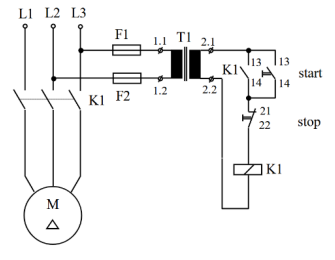
\includegraphics[width=0.5\textwidth]{assets/directeaanloop.png}
  \caption{Directe aanloop van de inductiemachine}
  \label{fig:directeaanloop.png}
 \end{figure}
\subsection{Stator serie weerstanden}
Hier gaan we regelbare weerstanden in serie zetten met de stator, bij opstarten maken we deze weerstanden maximaal zodat er een grotere spanningsval is over de weerstand ipv de motor, dit daalt het startkoppel en de startstroom dus. De weerstanden worden steeds lager gemaakt tot we op nominale spanning zijn. De weerstanden worden wel snel heel warm, deze moeten dus eigelijk gekoeld worden.
\begin{figure}[H]
  \centering
  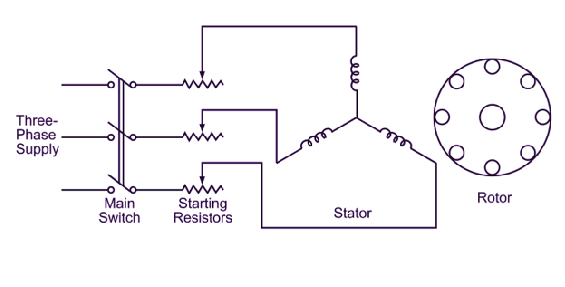
\includegraphics[width=0.6\textwidth]{assets/statorweerstandenserie.png}
  \caption{Stator serie weerstanden}
  \label{fig:statorweerstandenserie.png}
 \end{figure}
\subsection{Autotransformer (Spaartransformator)}
Een andere oplossing is opstarten met een spaartransformatie in serie met de motor, dit is eigelijk gelijkaardig aan die stator serie weerstanden, dit gebruikt echter spoelen om spanning te dempen, het verlagen van de opstartstroom en opstartkoppel is eigenlijk meer 'energetisch', je kan veel meer spanningsval hiermee creëren met veel minder vermogen verlies (want dit werkt met reactief vermogen). Maar het grote nadeel is wel dat het duur is.
\begin{figure}[H]
  \centering
  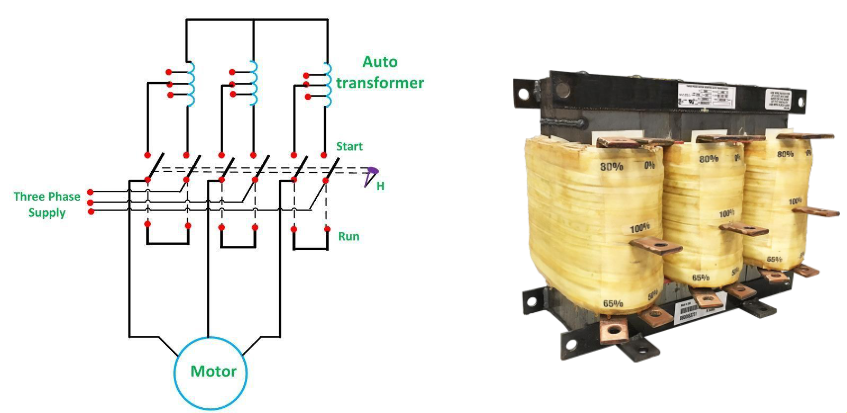
\includegraphics[width=0.6\textwidth]{assets/autotransforspaar.png}
  \caption{Autotransformer (Spaartransformator)}
  \label{fig:autotransforspaar.png}
 \end{figure}
\subsection{Softstarter}
Een softstarter is vermogenelektronica, het is meer geavanceerder en dus ook duurder. Het gebruikt thyristors (soort van diodes) in antiparallele posities (TRIACS), deze geleiden van zodra een signaal wordt gegeven op de gate. Hiermee kunnen we dus eigelijk geleidelijk aan de spanning verhogen door steeds meer van de sinus te laten doorlaten (steeds meer energie in de golf). Dit noemt eigelijk de 'ontsteekhoek' die we steeds kleiner maken. Dit kunnen we zien in de volgende figuur:
\begin{figure}[H]
  \centering
  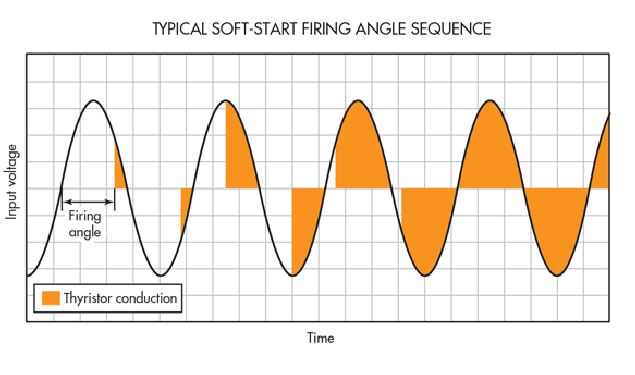
\includegraphics[width=0.6\textwidth]{assets/thyrsitorsinus.png}
  \caption{Softstarter met thyristors die geleidelijk de spanning verhogen}
  \label{fig:thyrsitorsinus.png}
 \end{figure}
\begin{figure}[H]
  \centering
  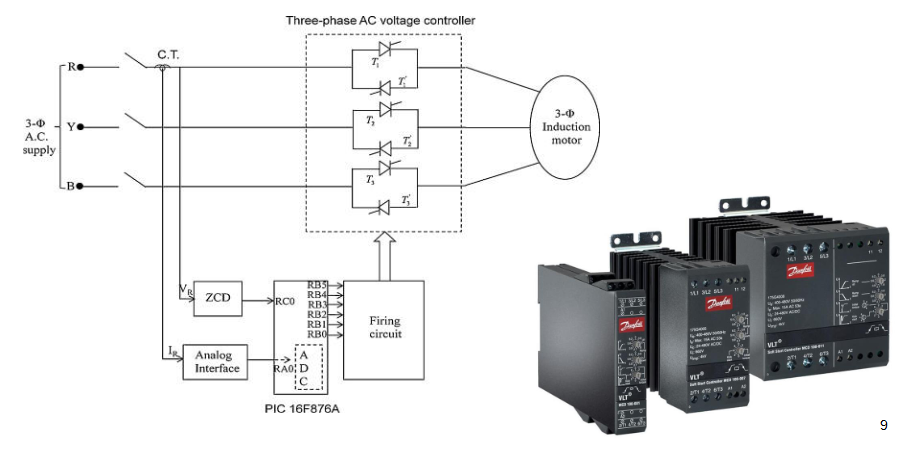
\includegraphics[width=0.6\textwidth]{assets/softstarterschakeling.png}
  \caption{Softstarter schakeling}
  \label{fig:softstarterschakeling.png}
 \end{figure}
Echter zorgt dit wel voor veel harmonischen (extra opwarming), maar dit is nog steeds beter dan hoge startstromen. Maar omdat het nog steeds warm is worden er koelvinnen op de softstarter geplaatst.
\subsection{Ster-driehoek starten}
De goedkoopste methode is ster-driehoek starten, hiervoor gebruik je gewoon een schakelaar en 2 contactoren (ookal zijn contactoren nog wel duur). We starten hierbij gewoon in ster, want in ster is de fasespanning lager ($V_f = \frac{V_L}{\sqrt{3}}$) en dus het startkoppel 3 keer lager (want $T \propto V_f^2 \propto \frac{V_L^2}{3}$). Het zelfde geld met de stroom want als je van ster naar driehoek gaat dan stijgt de spanning met $\sqrt{3}$ en de stroom ook met $\sqrt{3}$ dus samen stijgt de stroom met een factor van 3. (Dit is belangrijk om door te hebben!).
\begin{figure}[H]
  \centering
  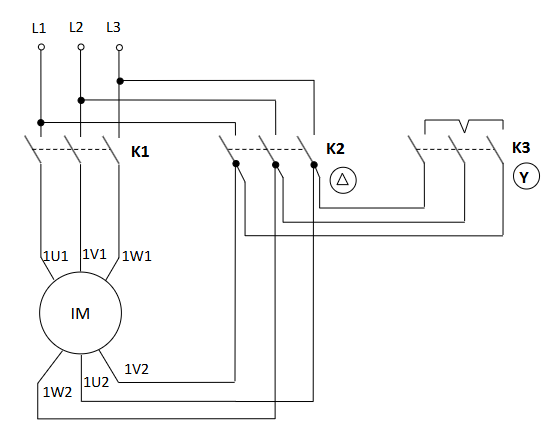
\includegraphics[width=0.5\textwidth]{assets/sterdriehoekstartenschakeling.png}
  \caption{Schakeling voor ster-driehoek starten}
  \label{fig:sterdriehoekstartenschakeling.png}
 \end{figure} 
Uiteindelijk willen we dus in driehoek werken, want zo zitten we op ons volledig vermogen. Op het moment van starten sluiten we K1 en K3, na een verloop van tijd gaan we EERST K3 openen (ster uitzetten) en dan K2 sluiten zodat we in driehoek zitten. We openen eerst K3 omdat we anders een kortsluiting op het net veroorzaken als we K2 sluiten als K3 nog gesloten is. Dit kan voorkomen worden dat dit gebeurd als we gewoon normally closed en normally open contactoren hiervoor gebruikt worden. Een nadeel is wel door dit te schakelen dat we eigelijk een transiënte krijgen, dit zien we in volgende karakteristiek voor ster en driehoek schakelen:
\begin{figure}[H]
  \centering
  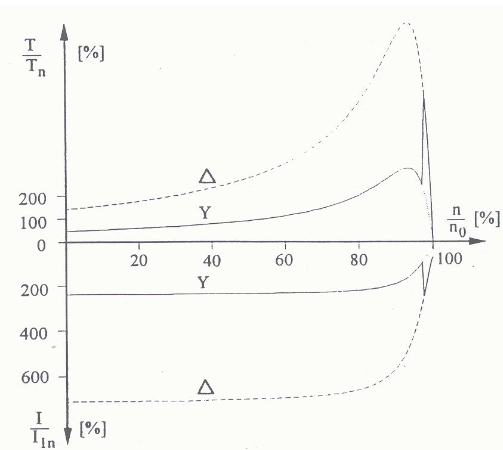
\includegraphics[width=0.5\textwidth]{assets/karakteristieksterdriehoekschakele.png}
  \caption{Karakteristiek van ster-driehoek schakelen}
  \label{fig:karakteristieksterdriehoekschakele.png}
 \end{figure}
Hier zien we deze transiente beter in een I-t karakteristiek:
\begin{figure}[H]
  \centering
  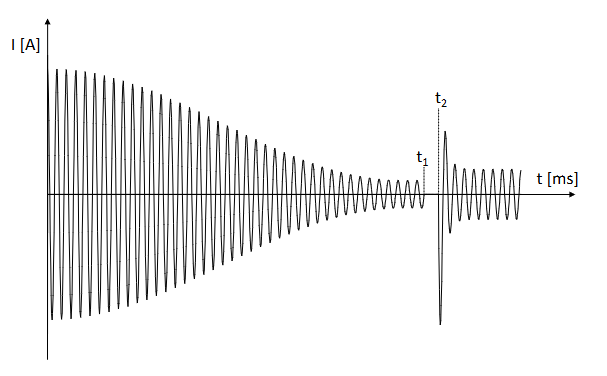
\includegraphics[width=0.6\textwidth]{assets/trabsiente.png}
  \caption{Transiënte karakteristiek bij ster-driehoek schakelen}
  \label{fig:trabsiente.png}
 \end{figure}
Dit kan verminderd worden door te werken met een tijdsvertraging.
\subsubsection{Vergelijken met DOL en Softstarter}
We gaan dan nu is de stroom en koppelkarakteristieken van de DOL, softstarter en ster-driehoek vergelijken. Dit zien we in de volgende figuur:
\begin{figure}[H]
  \centering
  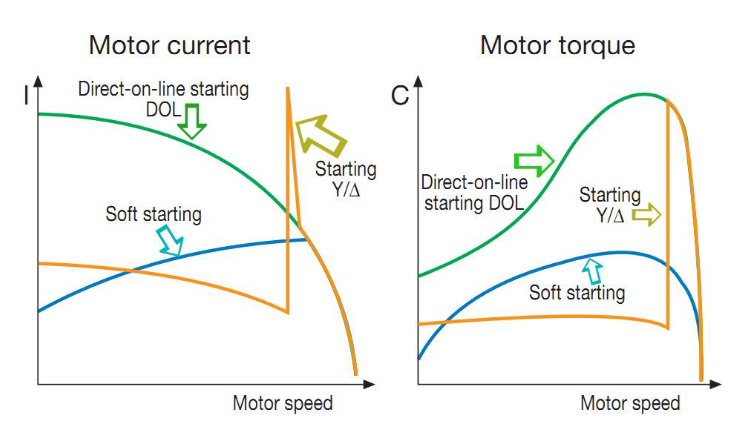
\includegraphics[width=0.6\textwidth]{assets/stroomkoppeldolsoftstartersterdriehoek.png}
  \caption{Stroom en koppelkarakteristieken van DOL, softstarter en ster-driehoek}
  \label{fig:stroomkoppeldolsoftstartersterdriehoek.png}
 \end{figure}
Nu zien we ook waarom softstarter 'soft' starter heet, je ziet dat de start voor de stroom en koppel mooi geleidelijk is, het heeft een vlak profiel. De ster-driehoek is een beetje vergelijkbaar maar je ziet hier wel duidelijk die transiënte waardoor het koppel eigelijk een lichte schok krijgt, wat je dus niet hebt bij de softstarter. (De proff meld wel nog dat de transiëntes hier een beetje overdreven getekend zijn)
\subsection{Externe rotorweerstanden}
Wat als we een hoge startkoppel willen maar geen hoge startstroom? Dan kunnen we gebruik maken van externe rotorweerstanden. Hiervoor is dus wel een gewonden rotor nodig (dit zagen we eerder, want hieraan kan je via sleepringen die weerstanden hangen). Bekijk nu eens volgende figuur:
\begin{figure}[H]
  \centering
  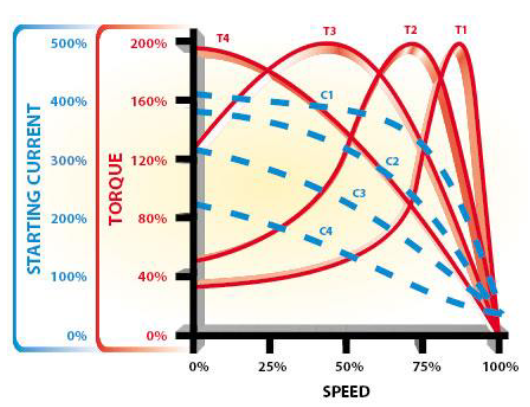
\includegraphics[width=0.6\textwidth]{assets/startstroomenstartkoppelbijverschillenderotorweerstanden.png}
  \caption{Startstroom en startkoppel bij verschillende rotorweerstanden}
  \label{fig:startstroomenstartkoppelbijverschillenderotorweerstanden.png}
 \end{figure}
Wat we gaan doen is dus beginnen bij T4, dit heeft dus een lage startstroom en hoog startkoppel, naarmate de snelheid toeneemt zullen het koppel en de stroom dus dalen. Wat we gaan doen is dan schakelen naar T3 (de volgende rotorweerstand), dit zorgt ervoor dat ons koppel niet begint te dalen maar ongeveer hetzelfde blijf, zelfde voor de stroom. Zo gaan we dan over naar T2 en dan naar T1. Dit zorgt dat we een langere tijd een hoog koppel hebben met een lage stroom. Dit is mogelijk volgens de formule voor $T_{ind}$ die we ook eerder zagen. Nadeel is dus dat je een gewikkelde rotor nodig hebt wat duur is, dit is niet toepasbaar bij een kooirotor. Een schema hiervan ziet er zo uit:
\begin{figure}[H]
  \centering
  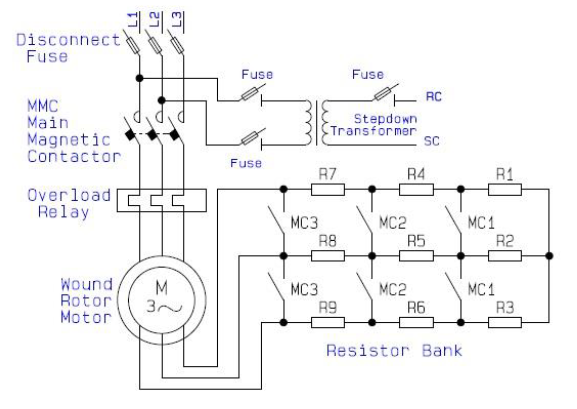
\includegraphics[width=0.5\textwidth]{assets/externerotorweerstandenschema.png}
  \caption{Schema van externe rotorweerstanden}
  \label{fig:externerotorweerstandenschema.png}
 \end{figure}
\subsection{Remmen van de inductiemachine}
Nu gaan we kijken naar het remmen van de inductiemachine. We hebben 5 soorten remmen voor de inductiemachine zonder gebruik te maken van externe remmen (dat niet gewoon uitbollen zijn). Deze zijn:
\begin{itemize}
    \item Plugging (tegenstroom remmen)
    \item DC-remmen
    \item Zero sequence braking (Homopolair remmen)
    \item Oversynchroon remmen
    \item Regeneratief remmen
\end{itemize}
\subsubsection{Plugging (tegenstroom remmen)}
Wat we hier gaan doen is eigelijk op ons stabiel werkingspunt de hoofdschakelaar uitschakelen en dan een andere schakeling aanzetten waarbij 2 fases omgedraaid zijn ten opzichte van de hoofdschakkelaar, zodat we eigelijk in het 4de kwadrant terecht komen in dissipatie, dit remt sterk af. We moeten hier wel zien dat we op tijd die schakelaar dan ook uitzetten want anders gaan we gewoon in de andere richting versnellen. Dit wordt vooral toegepast als we snel gestopt kunnen raken en niet te veel moeten stoppen want dit warmt veel op door die dissipatie.
\begin{figure}[H]
  \centering
  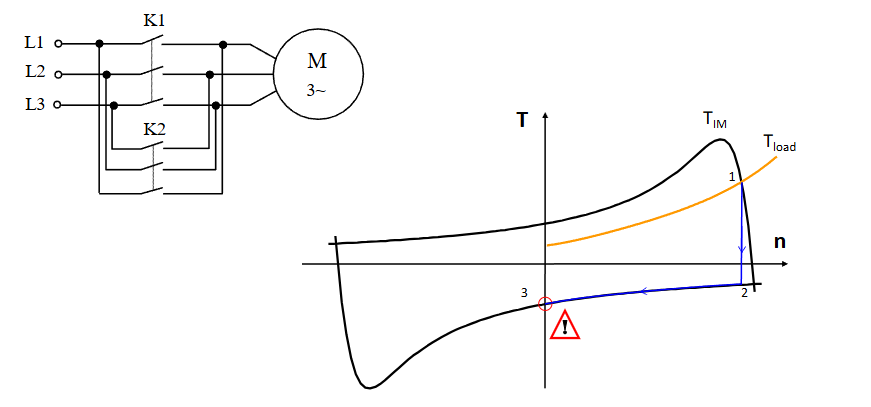
\includegraphics[width=0.6\textwidth]{assets/tegenstroomremmen.png}
  \caption{Tegenstroomremmen}
  \label{fig:tegenstroomremmen.png}
 \end{figure}
Dit is de goedkoopste remmethode, het heeft een 2de contactor nodig. Om te checken dat je op tijd de andere contactor sluit zodat je niet versnelt gebruiken we een 'ruwe' snelheidsdetectie, deze heeft een accuraatheid dat 50 tr/min kan schelen.
\subsubsection{DC-remmen}
Deze methode wordt minder gebruikt omdat een gelijkstroomrichter nodig is dat wat duurder is, maar bij niet te grote vermogens valt dit goed mee. Wat we hier gaan doen is met een gelijkstroombron (DC) een gelijkstroom aanleggen op 2 windingen zodat we in de stator een constant magnetisch veld krijgen (dus geen draaiveld), dit gaat in de rotor een spanning induceren dat een stroom veroorzaakt en dus een koppel genereert dat tegengesteld is aan de draairichting van de rotor. Dit remt dus af. Wat we ook zien is dat dit koppel toeneemt naarmate de rotor afremt en dat deze gelijk is aan 0 als de snelheid 0 is, dit lost dus het probleem van de vorige methode op.
\begin{figure}[H]
  \centering
  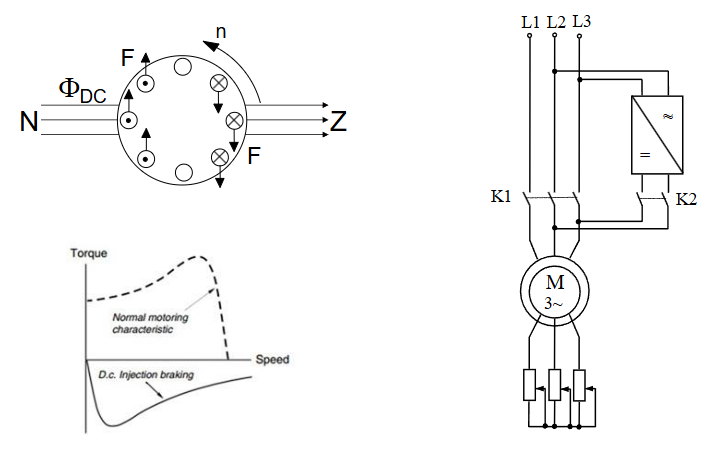
\includegraphics[width=0.5\textwidth]{assets/DCremmen.png}
  \caption{DC-remmen}
  \label{fig:DCremmen.png}
 \end{figure}
\subsubsection{Zero sequence braking (Homopolair remmen)}
Dit is maar kort besproken in de les, maar wat we hier doen is de motor loskoppelen van het net en de 3 statorwikkelingen aansluiten zodat ze allemaal exact dezelfde stroom met dezelfde fase (homopolair) krijgen want tegenover de draaiened rotor geeft dit netto een afremmend koppel die we eerder zagen.
\subsubsection{Oversynchroon remmen}
Dit wordt eigelijk minder als remmen beschouwt, dit is eerder om te voorkomen dat iets beweegt of te snel gaat. Vooral gebruikt in liften/kranen. Bij lasten laten zakken gaan we eigelijk gewoon in generatorwerking gaan en dus een negatief koppel krijgen wat doet afremmen. Potentiele energie wordt dus terug omgezet in elektrische energie, dit maakt het een soort van generatief remmen.
\begin{figure}[H]
  \centering
  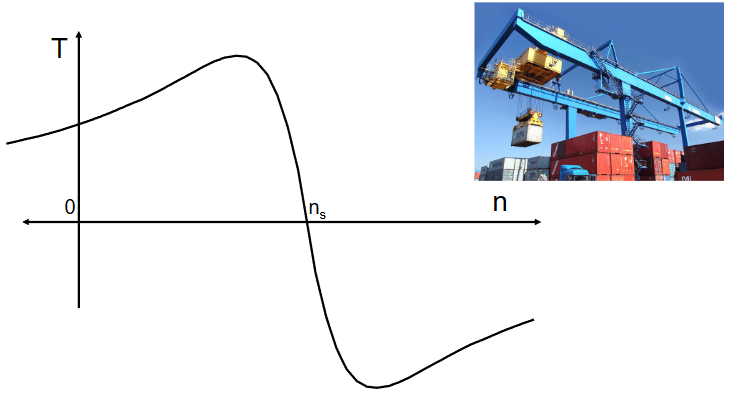
\includegraphics[width=0.5\textwidth]{assets/oversynchroonremmen.png}
  \caption{Oversynchroon remmen}
  \label{fig:oversynchroonremmen.png}
 \end{figure}
\subsubsection{Regeneratief remmen}
Hierbij gaan we echt remmen door gebruik te maken van de generatorwerking van de inductiemachine. Hiervoor moeten we de synchrone snelheid verlagen zodat de curve naar links opschuift zoals je ziet in de figuur. De rotor beweegt zo sneller als het magnetisch veld wat dus generator werking veroorzaakt. Dit gaan we doen door de flux constant te houden en de frequentie aanpassen met een frequentieregelaar. Maar omdat frequentie aanpassen het veld aanpast (dat we constant willen houden) gaan we samen de spanning met de frequentie doen dalen want $E \approx V_\phi$ en dit doen we dan stap per stap.
\begin{figure}[H]
  \centering
  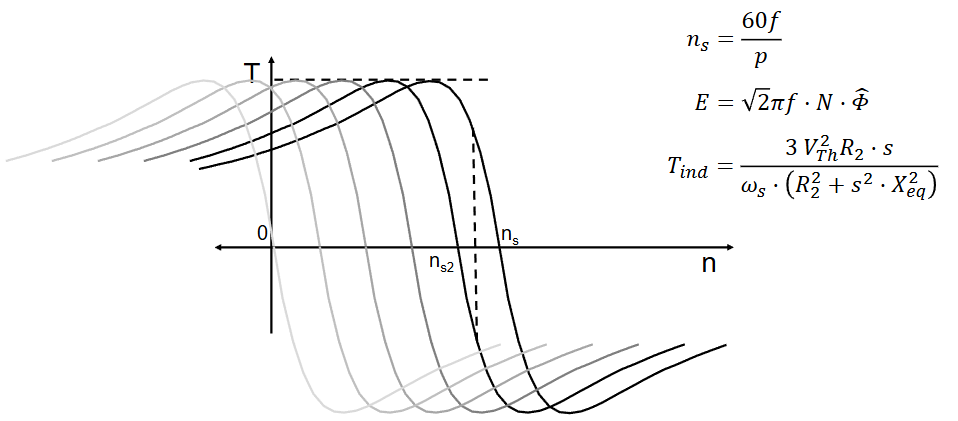
\includegraphics[width=0.7\textwidth]{assets/regeneratiefremmen.png}
  \caption{Regeneratief remmen}
  \label{fig:regeneratiefremmen.png}
 \end{figure}
\subsection{Generatorwerking van de inductiemachine}
Nu gaan we eens kijken naar de generatorwerking van de inductiemachine. Het is het gedeelte $\frac{R_2}{s}$ dat ervoor zorgt dat als we negatieve slip hebben dat er energie geleverd wordt door magnetisch veld naar de stator. We gaan eens kijken naar een wind turbine:
\begin{figure}[H]
  \centering
  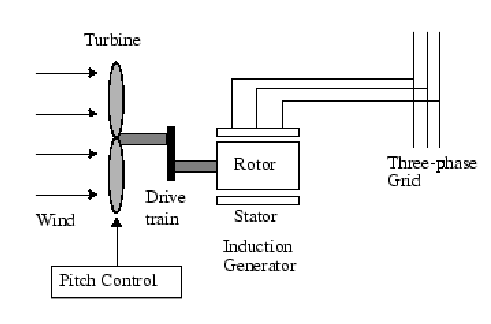
\includegraphics[width=0.5\textwidth]{assets/windturbinevoorbeeld.png}
  \caption{Windturbine voorbeeld}
  \label{fig:windturbinevoorbeeld.png}
 \end{figure}
Dit is een grote generator, wat het doet is eigelijk actief vermogen tot het net brengen. De motor kan alleen actieve energie leveren terwijl de rotor ook reactief vermogen nodig heeft in de wikkelingen voor het veld te maken, het moet dit dus van het net trekken, daarvoor worden condensator banken gebruikt, deze verminderen het reactief vermogen dat we van het net moeten nemen. De reden dat dit met een asynchrone en niet een synchrone machine is, is omdat dit niet op een constante snelheid werkt. Ook is er nog een overbrenging om de rotatie naar een ideale snelheid voor de motor te brengen.
\subsubsection{Singly Fed}
Dit is het normale geval, enkel de stator is hier elektrisch aan het net gesloten. De rotor krijgt stroom via inductie. Dit is gewoon de standaard generator werking die we eerder zagen.
\begin{figure}[H]
  \centering
  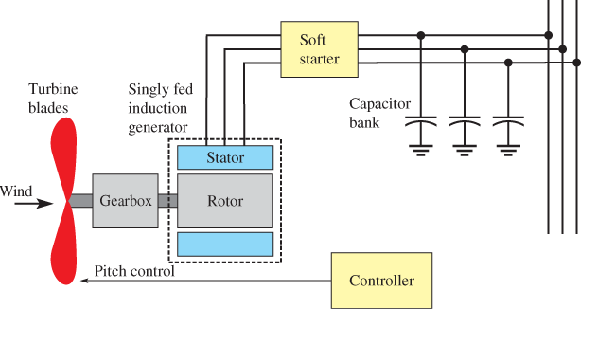
\includegraphics[width=0.6\textwidth]{assets/singlyfed.png}
  \caption{Singly Fed}
  \label{fig:singlyfed.png}
 \end{figure}
\subsubsection{Doubly Fed}
Dit is al wat anders. Hier beide wikkelingen elektrisch aangesloten. Zowel de stator als rotor aan het net dus. We gaan zoveel mogelijk actief vermogen naar het net sturen. Voor de rotor wordt hier vermogenelektronica en rotor weerstanden gebruikt zodat je een optimaal koppel behoudt en zoveel mogelijk naar het net kan sturen. Dit is veel efficiënter.
\begin{figure}[H]
  \centering
  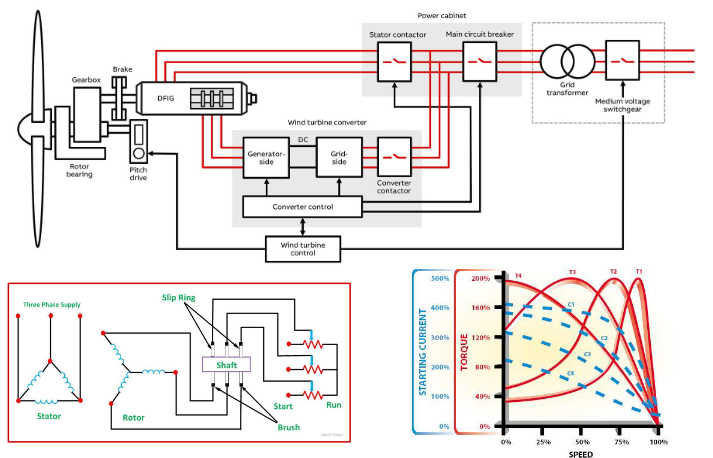
\includegraphics[width=0.6\textwidth]{assets/doublyfed.png}
  \caption{Doubly Fed}
  \label{fig:doublyfed.png}
 \end{figure}
\subsection{Oefeningen}
\begin{oefenblok}[Oefening 6-26 Slides]
    \textbf{Opgave:}
    \newline
    A 460V 50hp (=37kW) six-pole $\Delta$-connected 60Hz threephase induction motor has a full-load slip of 4\%, an efficiency of 91\% and a power factor of 0.87 lagging. At start-up the motor develops 1.75 times the full-load torque but draws 7 times the rated current at the rated voltage. This motor is to be started at reduced voltage using a softstarter.
\begin{itemize}
 \item a) What should be the output voltage of the softstarter to reduce the starting torque until it equals the rated torque of the motor?
 \item b) What will the motor starting current be at this voltage?
 \item c) And what is the current drawn from the supply?
\end{itemize}
   \textbf{Oplossing:}
   \newline
   \dots ({\color{red}Nog niet aan begonnen})
\end{oefenblok}
\begin{oefenblok}[Excercise Induction motor Slides]
    \textbf{Opgave:}
    \begin{figure}[H]
      \centering
      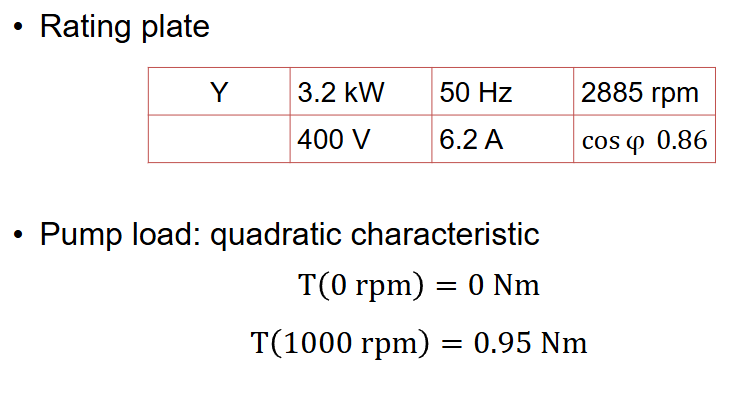
\includegraphics[width=0.6\textwidth]{assets/opgaveIMoefening.png}
      \caption{Opgave Inductie Motor}
      \label{fig:opgaveIMoefening.png}
     \end{figure}
    \begin{itemize}
     \item a) Nominal operation point $\rightarrow n_s, n_{nom}, s_{nom}, P_{el}, P_{mech}, \eta, T_{nom}$
     \item b) Load $\rightarrow$ operation point
     \item c) Voltage dip $\Delta U_l = 80 V \rightarrow$ torque?
    \end{itemize}
    \textbf{Oplossing:}
    \newline
    \dots ({\color{red}Nog niet aan begonnen})
\end{oefenblok}
\begin{oefenblok}[Oefening 1 - Slip (Toledo)]
    \textbf{Opgave:}
    \newline
    Slip and speed are related. Complete the drawing by naming the slip axis (pink) and adding some interesting values.
    \begin{figure}[H]
      \centering
      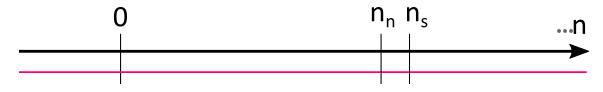
\includegraphics[width=0.6\textwidth]{assets/opgaveSlip.png}
      \caption{Opgave Slip}
      \label{fig:opgaveSlip.png}
     \end{figure}
    \textbf{Oplossing:}
    \newline
    \dots ({\color{red}Nog niet aan begonnen})
\end{oefenblok}

\begin{oefenblok}[Oefening 2 - Rating plate (Toledo)]
    \textbf{Opgave:}
    \newline
    Questions:
    \begin{itemize}
     \item 1. number of pole sets, synchronous speed, nominal slip, efficiency, nominal torque
     \item 2. if the torque is only $T_{nom}/2$, determine the delivered power
     \item 3. at which speed will the machine rotate if it is driven at $T=25\,Nm$?
    \end{itemize}
    Numerical answers:
    \begin{itemize}
     \item 1. 2, 1500rpm, 4\%, 81\%, 37Nm
     \item 2. 2.8kW
     \item 3. 1545rpm
    \end{itemize}
    \textbf{Oplossing:}
    \newline
    \dots ({\color{red}Nog niet aan begonnen})
\end{oefenblok}

\begin{oefenblok}[Oefening 3 - Equivalent circuit (Toledo)]
    \textbf{Opgave:}
    \newline
    Determine the equivalent circuit of an induction machine, supplied by the grid $3\times400V@50Hz$, with following rating plate and measurements:
    \begin{itemize}
     \item Rating plate: 400V; 50Hz; 533A; $\cos\varphi$ 0.89; 315kW; 2980rpm
     \item No load: $I_0 = 124.7\,A$; $P_0 = 5.73\,kW$;
     \item Locked rotor: $U_{lr} = 66.1\,V$; $P_{lr} = 16.3\,kW$;
     \item Full load: $P_{in} = 327.5\,kW$; $P_{out} = 315\,kW$;
     \item Resistance between lines = $4.4\,m\Omega$
    \end{itemize}
    Numerical answers: $R_1=2.2\,m\Omega$, $X_1=61\,m\Omega$, $X_2=61\,m\Omega$, $R_2=17\,m\Omega$, $R_c=28\,\Omega$, $X_m=1.8\,\Omega$
    \newline
    \textbf{Oplossing:}
    \newline
    \dots ({\color{red}Nog niet aan begonnen})
\end{oefenblok}

\begin{oefenblok}[Oefening 5 - Pump load (Toledo)]
    \textbf{Opgave:}
    \newline
    Given:
    \begin{itemize}
     \item Rating plate: 3.2kW, 50Hz, 2885rpm, 400V (Y), 6.2A, $\cos\varphi$ 0.86
     \item neglect stator losses, iron losses
     \item $I_0=2.8\,A$, $L_{leakage}=4.5\,mH$
     \item load: pump (quadratic characteristic, $T_{pump}=0.95\,Nm$ at 1000rpm)
    \end{itemize}
    Questions:
    \begin{itemize}
     \item 1. Determine: $n_s, n_{nom}, s_{nom}, P_{el}, P_{mech}, \eta_{nom}$
     \item 2. the (simplified) equivalent circuit: elements, voltages and currents. Draw the phasor diagram too
     \item 3. Determine the operating point when driving the pump (torque and speed)
     \item 4. For a voltage dip of 80V, determine the motor torque.
    \end{itemize}
    \textbf{Oplossing:}
    \newline
    \dots ({\color{red}Nog niet aan begonnen})
\end{oefenblok}

% ==================================================================

% ==================================================================
\newpage
\chapter{Motorselectie}
% Inhoud volgt
Nu gaan we kijken naar hoe we kunnen bepalen welke motor we nodig hebben voor een bepaalde toepassing. Dit kan afhangen van applicatie, beschikbare catalogus, standaarden (normen, vind je ook op kenplaat zoals bvb. IEC 60034), dimensionering, $\cdots$
\begin{figure}[H]
  \centering
  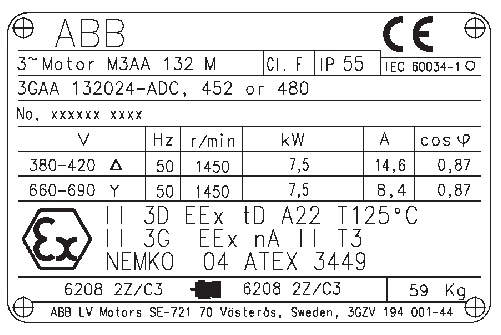
\includegraphics[width=0.6\textwidth]{assets/kenplaatmetnorm.png}
  \caption{Kenplaat met norm IEC 60034}
  \label{fig:kenplaatmetnorm.png}
 \end{figure}
Op deze kenplaat zien we vanalle dingen die we zometeen nog verder zullen bespreken, ik wil het nu even hebben over die IEC 60034, dit is een norm van de \textbf{Internationale Elektrotechnische Commitee}, zij hebben normen over zo goed als alles wat elektrisch is zoals bvb. energiecurves en efficiëntieklassen. Er is ook nog een Amerikaanse versie, hier hebben we het al eerder over gehad, namelijk de \textbf{NEMA}.
\begin{figure}[H]
  \centering
  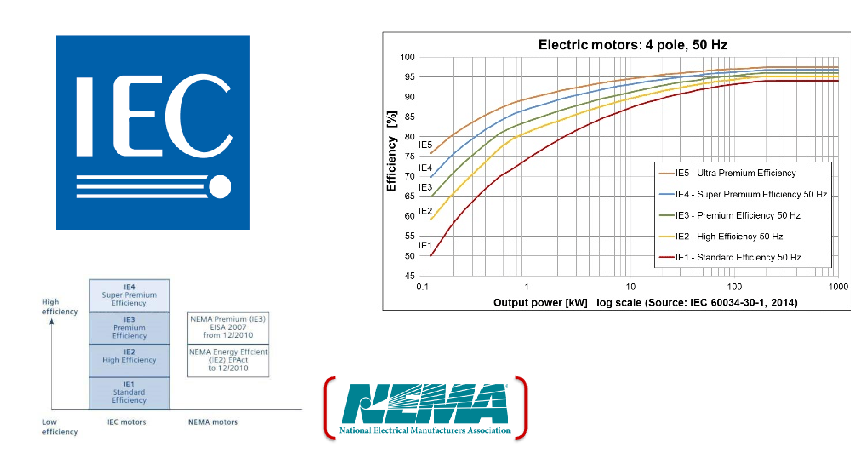
\includegraphics[width=0.6\textwidth]{assets/standaarden.png}
  \caption{IEC en NEMA}
  \label{fig:standaarden.png}
 \end{figure}
\subsection{IP-klasse}
Iets wat we eigelijk al veel hebben gezien maar hier dus ook voorkomt zijn de zogenaamde IP-klassen, IP staat voor \textit{Index of Protection}. Een IP-klasse is altijd een nummer met 2 cijfers, het eerste cijfer toont de bescherming tegen vaste voorwerpen en het tweede cijfer de bescherming tegen vloeistoffen. Hoe hoger het cijfer hoe beter de bescherming. Hier is een overzicht van de IP-klassen:
\begin{figure}[H]
  \centering
  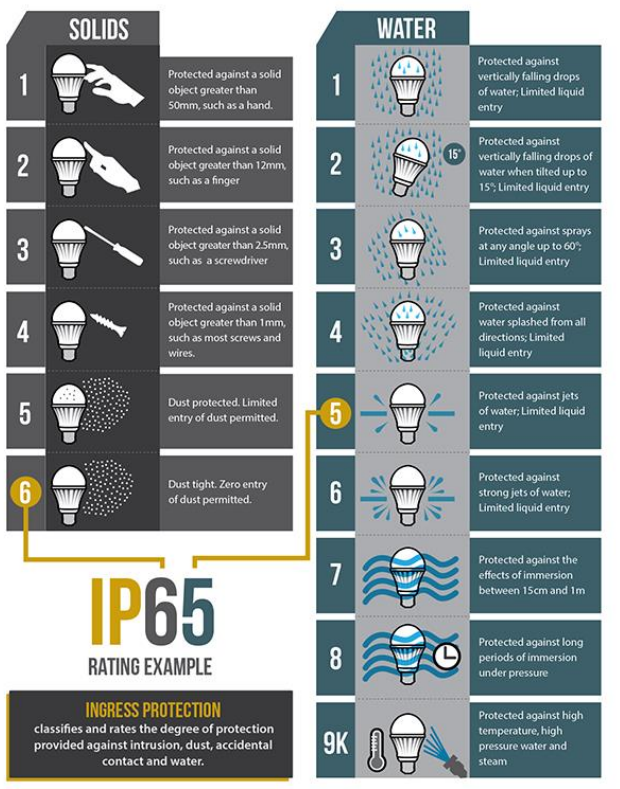
\includegraphics[width=0.4\textwidth]{assets/IPklassennummers.png}
  \caption{IP-klassen}
  \label{fig:IPklassennummers.png}
 \end{figure}
Een IP23 zoals de gele motor is dan dus bescherm tegen iets grotere voorwerpen, dus je vingers kunnen er niet tussen maar lucht en stof kan dus binnen. Een IP55 zoals de blauwe motor is juist helemaal dicht en kan tegen waterstralen.
\begin{figure}[H]
  \centering
  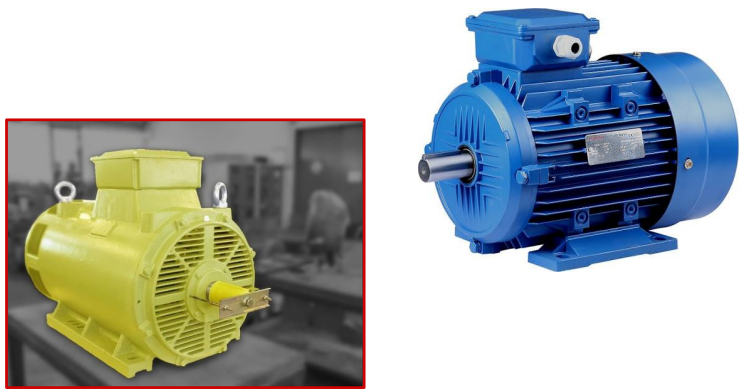
\includegraphics[width=0.5\textwidth]{assets/geleenblauwemotor.png}
  \caption{Gele en blauwe motor met IP23 en IP55}
  \label{fig:geleenblauwemotor.png}
 \end{figure}
\subsection{Isolatieklassen}
Ook hebben we isolatieklassen, deze duiden aan hoe warm de isolatie van de motor mag worden (op nominale stroom). Dit is belangrijk om zicht over te hebben want materiaal verouderd bij hogere temperaturen. Deze klassen worden opgesteld door te kijken naar welk onderdeel van de machine het eerste faalt, want brand willen we absoluut vermijden. De onderstaande grafiek toont de maximale temperaturen (voor op nominale stroom) dat je machine mag worden bij die bepaalde klasse (A,E,B,F,H) met H de beste dus.
\begin{figure}[H]
  \centering
  
\includegraphics[width=0.6\textwidth]{assets/isolatieklassen.png}
  \caption{Isolatieklassen}
  \label{fig:isolatieklassen.png}
 \end{figure}
\subsection{Nominaal werkingspunt vs. echt werkingspunt}
{\color{red}(Dit stukje is deels door AI geschreven op basis van mijn lesnotities, ik heb nagekeken en het klopt allemaal en is effectief allemaal aan bod gekomen in de les)}
\newline
\newline
Voor motorselectie kijk je best niet alleen naar het nominaal werkingspunt op de kenplaat, want in de praktijk draait de motor vaak op een lagere belasting (echt werkingspunt). Zowel het rendement als de arbeidsfactor zijn namelijk geen constante kenplaatwaarden, maar hangen sterk af van de belastingsgraad. Bij nullast geldt $\eta=P_{mech}/P_{el}\to 0$: er is geen nuttig mechanisch vermogen ($P_{mech}=0$), maar wel nog steeds verliezen (ijzer-, wrijvings- en magnetiseerverliezen), dus $P_{el}>0$. De arbeidsfactor daalt echter veel sterker bij deellast dan het rendement. Dit komt doordat het reactief vermogen $Q$ (nodig voor de magnetisatie, via $X_m$) nauwelijks verandert met de belasting, terwijl het actief vermogen $P$ wel sterk daalt. Aangezien $\cos\varphi=P/S=P/\sqrt{P^2+Q^2}$, zakt $\cos\varphi$ hierdoor snel naarmate de belasting afneemt (tot ongeveer $0{,}2-0{,}4$ bij nullast). Dit is dan ook een belangrijke reden om een motor niet te overdimensioneren: bij een motor die permanent ver onder zijn nominaal vermogen draait, zakt de arbeidsfactor sterk, wat extra reactief vermogen van het net vraagt zonder bijkomend nuttig vermogen. Op de volgende grafiek zien we dan hoe het rendement en de arbeidsfactor afnemen naarmate de motor meer belast wordt, dit is dus uitgezet met een verticale reductiecoëficiënt:
\begin{figure}[H]
  \centering
  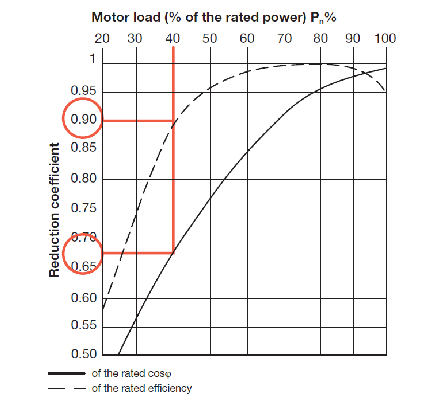
\includegraphics[width=0.4\textwidth]{assets/reductierendementenarbeidsfactor.png}
  \caption{Grafiek reductie van rendement en arbeidsfactor bij deellast}
  \label{fig:reductierendementenarbeidsfactor.png}
 \end{figure}
Het rendement is hier eigelijk uitgedrukt als $\frac{\eta}{\eta_{nom}}$ en de arbeidsfactor als $\frac{\cos\varphi}{\cos\varphi_{nom}}$. Wat we dus ook zien is dat het rendement naar 0 gaat bij nullast. En in het begin de snelheid het hoogste is, het is dus hoger bij deellast dan vollast.
\subsection{Werkingsregimes of Intermiteair gedrag}
Dan kunnen we ook nog classificeren hoe de motor belast kan worden in de tijd, wat bepaalt hoe de motor moet worden gekoeld of gewoon tot hoelang de motor kan werken. Classificaties hiervan worden aangeduid met S en dan een getal erachter van S1 tot S8, een paar voorbeelden zijn in de les gezien en zal ik nu overlopen.
\begin{figure}[H]
  \centering
  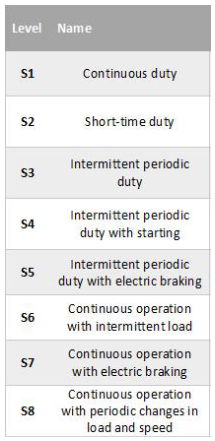
\includegraphics[width=0.25\textwidth]{assets/werkingsregimes.png}
  \caption{Werkingsregimes klassen S1 tot S8}
  \label{fig:werkingsregimes.png}
 \end{figure}
Klasse S1 ziet er als volgt uit:
\begin{figure}[H]
  \centering
  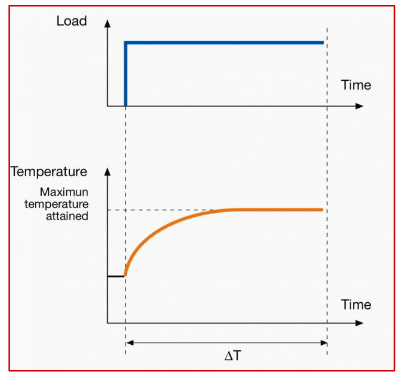
\includegraphics[width=0.35\textwidth]{assets/S1.png}
  \caption{S1 werkingsregime}
  \label{fig:S1.png}
 \end{figure}
Hier zet je de motor aan en laat je hem aan staan op het zelfde vermogen, het duurt even tot de temperatuur op regimetemperatuur komt maar daarna veranderd die niet, deze klasse kan dus gewoon constant blijven in de tijd. In de onderstaande figuur de S3 klasse:
\begin{figure}[H]
  \centering
  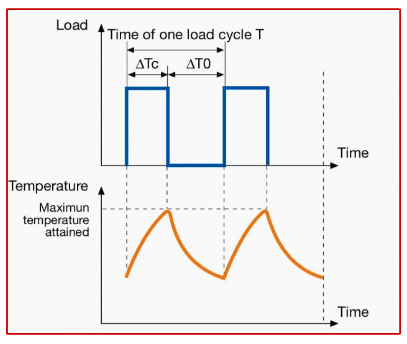
\includegraphics[width=0.35\textwidth]{assets/S3.png}
  \caption{S3 werkingsregime}
  \label{fig:S3.png}
 \end{figure}
Wat we hier dan zien is dat we de motor aanzetten, deze gaat opwarmen tot een bepaalde temperatuur en dan gaan we hem uitzetten, hij gaat dan afkoelen. Dit gaan we dan herhalen, dit kan dus een aantal keer na elkaar. Het is dus een intermitent gedrag (periodisch), het kan niet constant blijven werken. En de laatste dat is besproken is dan S4:
\begin{figure}[H]
  \centering
  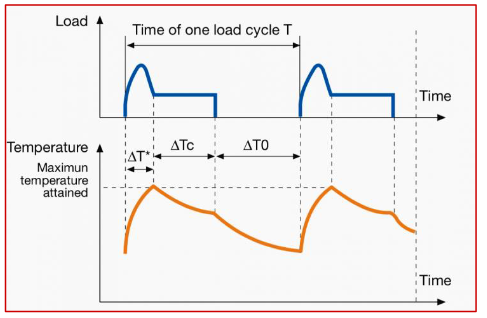
\includegraphics[width=0.4\textwidth]{assets/S4.png}
  \caption{S4 werkingsregime}
  \label{fig:S4.png}
 \end{figure}
Hier was niet echt uitleg over in de les gegeven dus deze ga ik niet in detail verder bespreken.
\subsection{Explosie veilig materiaal}
Er zijn ook coderingen afhankelijk van je werkingsomgeving, zoals bijvoorbeeld explosieveilig materiaal. Dit is belangrijk in de chemische industrie waar er veel gassen en dampen zijn die kunnen ontbranden. Hier zijn dan ook speciale motoren voor nodig die dit kunnen weerstaan. Deze worden aangeduid met een lettercode, deze kan je terugvinden op de kenplaat van de motor.
\begin{figure}[H]
  \centering
  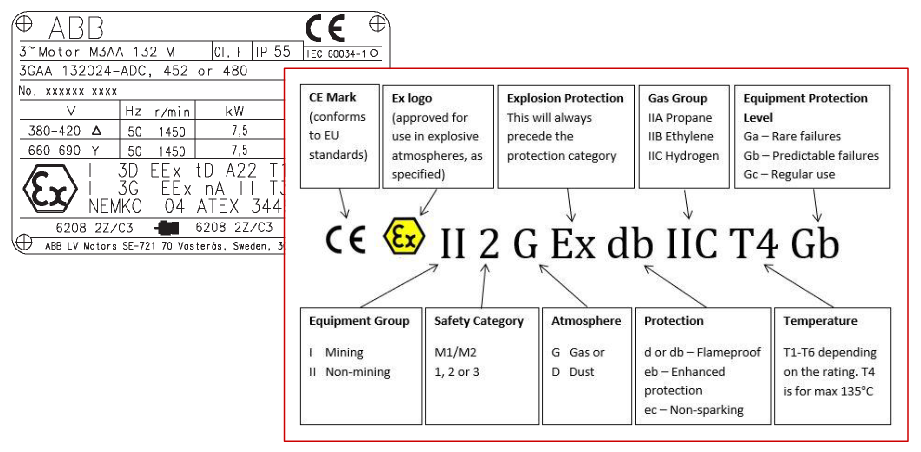
\includegraphics[width=0.6\textwidth]{assets/explosiecodering.png}
  \caption{Explosieveilige codering van motoren}
  \label{fig:explosiecodering.png}
 \end{figure}
\subsection{Bouwvorm}
Bouwvorm is ook iets dat wordt weergegeven op de kenplaat, typisch met een B en dan een getal voor horizontale assen en een V en een getal voor verticale assen. Dit is handig want na 15 jaar ofzo kan je dan bvb. van motor veranderen in je machine en kan je gewoon een motor van een andere type of merk nemen zolang dat die bouwvorm hetzelfde is, het past dan nog steeds in je machine.
\begin{figure}[H]
  \centering
  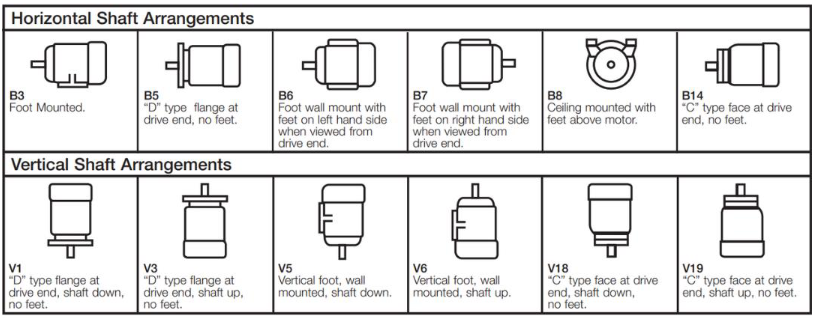
\includegraphics[width=0.8\textwidth]{assets/bouwvorm.png}
  \caption{Bouwvormen van motoren}
  \label{fig:bouwvorm.png}
 \end{figure}
\subsection{Motor Catalogus}
Het echt 'kiezen' van de motor doen we met een motorcatalogus, hierin zie je meerdere gegevens die niet op de kenplaat staan, verschillende lastbedrijven, kipkoppels, geluid, $\cdots$
\begin{figure}[H]
  \centering
  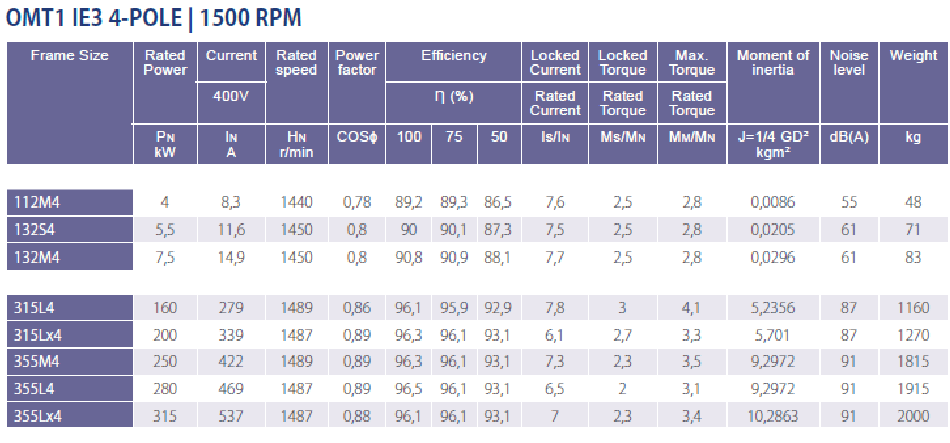
\includegraphics[width=0.8\textwidth]{assets/voorbeeldmotorcatalogus.png}
  \caption{Voorbeeld van een motorcatalogus}
  \label{fig:voorbeeldmotorcatalogus.png}
 \end{figure}
We zien hier ook die 'rated power', dit is meestal het belangrijkste gegeven dat je nodig hebt om te kijken of de motor geschikt is voor je toepassing. Daar bij het rendement zie je de efficientie voor vollast, deellast en halflast. Zelfs de stroom bij blokkeren (stilstand) staat hier op.
\subsection{Motor dimensionering}
Dan gaan we nu kijken naar hoe we onze motor zelf kunnen dimensioneren, sommige dingen bereken je zelf, sommige dingen hangen af van je toepassing. Verschillende bepalende factoren zijn:
\begin{itemize}
    \item \textbf{Vermogen} van de motor, dit zelf hangt dan nog is af van de \textbf{snelheidsrange} en je \textbf{koppel} (\textit{nominaal, kip en 'houd' koppel }(dit is bij stilstand, vooral handig bij stappenmotoren gewoon))
    \item Directe aandrijving of via een \textbf{transmissie} (bvb. tandwielkast, riem, $\cdots$)
    \item \textbf{Werkingsregime} (S1, S2, $\cdots$)
    \item \textbf{Beschikbare voeding} (je kan bvb. een 1f of 3f voeding hebben van een bepaalde spanning)
    \item \textbf{Coupling} (mechanisch, hydraulisch, $\cdots$)
    \item \textbf{Mounting} (hangt dus eigelijk af van de \textbf{bouwvorm} van de motor)
    \item \textbf{Omgeving} (explosieveilig, stof, vocht, $\cdots$)
    \item \textbf{Prijs!}
\end{itemize}
\subsubsection{Voorbeeldoefening Roller}
Stel we hebben een toepassing waarbij we eigelijke een materiaal willen walsen met 2 rollers, we willen dan weten wat voor motor we nodig hebben. Met de afmetingen en snelheden gegeven zoals in volgende figuur gaan we dan nu eens bepalen wat voor motor we nodig hebben.
\begin{figure}[H]
  \centering
  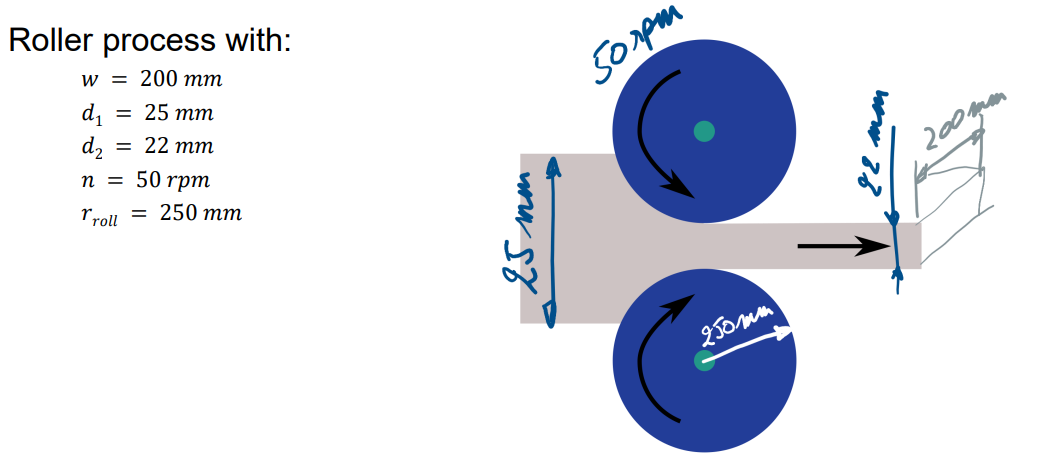
\includegraphics[width=0.8\textwidth]{assets/rolleroef.png}
  \caption{Roller oefening}
  \label{fig:rolleroef.png}
 \end{figure}
\begin{figure}[H]
  \centering
  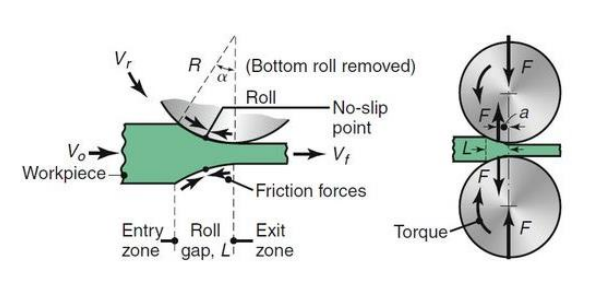
\includegraphics[width=0.6\textwidth]{assets/werkingroller.png}
  \caption{Krachtendiagram rollers}
  \label{fig:werkingroller.png}
 \end{figure}
De slides geven hier nog bij dat er een contact lengte is van 27.4mm (dit komt van $L = \sqrt{R \cdot \Delta d} = \sqrt{250mm \cdot (25mm - 22mm)}$ maar moeten we niet kennen) en een gemiddelde vloeispanning van 176 MPa. Met een rare walskracht formule die we niet moeten kennen wordt een kracht van $F = 962 kN$ gevonden en kan hiermee het koppel van de rollers bepaald worden:
\begin{align*}
    T_{roll} = F \cdot \frac{L}{2} = 962 kN \cdot \frac{27.4 mm}{2} = 13.2 kNm
\end{align*}
Dit is dus het koppel \textit{per} rol. Als we beide rollers met dus dezelfde motor aandrijven dan is het totale vermogen nodig voor die motor:
\begin{align*}
    P_{tot} = 2 \cdot T_{roll} \cdot \omega_{roll} = 2 \cdot 13.2 kNm \cdot 2\pi \cdot \frac{50 rpm}{60} = 138 kW
\end{align*}
Als we nu nog rekening houden met een rendement van 0.9 dan kunnen we dit theoretisch mechanisch vermogen omzetten in elektrisch vermogen dat we nodig hebben:
\begin{align*}
    P_{el} = \frac{P_{tot}}{\eta} = \frac{138 kW}{0.9} = 153 kW
\end{align*}
We hebben dus een motor nodig van 153 kW, in de onderstaande catalogus komt dit overeen met de rode omkaderde motor. We zien hier wel dat deze een nominale snelheid van 993 tr/min heeft, dus hebben we een overbrenging nodig.
\begin{figure}[H]
  \centering
  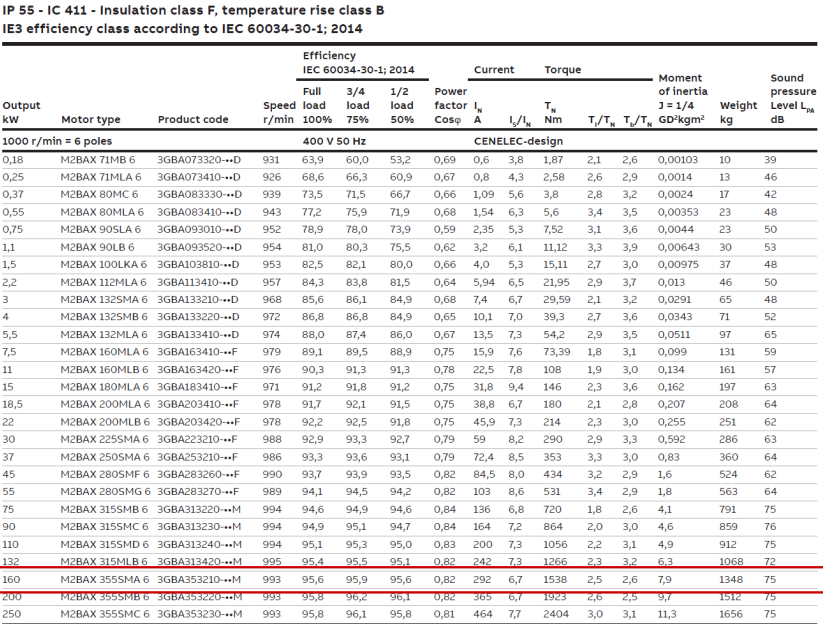
\includegraphics[width=0.6\textwidth]{assets/motorcatalogusroller.png}
  \caption{Motor Catalogus}
  \label{fig:motorcatalogusroller.png}
 \end{figure}
In een aandrijving zijn meerdere rendementen eigelijk, we hebben ons rendement van de motor ($\eta_{mot}$), het rendement van de transmissie ($\eta_{tr}$) en het rendement van de load ($\eta_{load}$). Die van de motor zelf gebruiken we eigelijk niet om de motor te kiezen, we gebruiken die van de load, dit is eigelijk het totale rendement. Het echt weten van welk rendement je nodig hebt en wanneer behoort wel niet tot deze cursus, dit is iets wat je ziet in het vak Dimensionering van Machines.
% Zorg dat dit in je preamble staat (waarschijnlijk al aanwezig):
% \usepackage{graphicx}
% \usepackage{tikz}
% \usetikzlibrary{shapes.geometric, arrows.meta, calc, positioning}

\begin{figure}[h]
\centering
\resizebox{\textwidth}{!}{%
\begin{tikzpicture}[
    font=\sffamily,
    circnode/.style={circle, draw=black, thick, minimum size=2.1cm,
        align=center, font=\sffamily\bfseries},
    blocknode/.style={rectangle, draw=black, thick, minimum width=1.0cm},
    loadnode/.style={rectangle, rounded corners=8pt, draw=black, thick,
        minimum width=2.7cm, minimum height=2cm,
        align=center, font=\sffamily\bfseries},
    Pbox/.style={rectangle, draw=black, fill=magenta!12,
        minimum width=1.2cm, minimum height=0.65cm, font=\small,
        align=center, inner sep=1pt},
    etabox/.style={rectangle, draw=black!70, fill=green!12,
        minimum width=1.2cm, minimum height=0.65cm, font=\small,
        align=center, inner sep=1pt},
]

% ---------- Bovenste rij: Grid - IM - Transmission (bovenste helft) ----------
\node[circnode, fill=orange!35]                (grid) at (0,3)   {Grid};
\node[circnode, fill=red!70!black, text=white] (im)   at (4.4,3) {IM};
\node[blocknode, fill=cyan!55!blue!35, minimum height=1.3cm] (trans1) at (7.6,3) {};

% ---------- Onderste rij: Transmission (onderste helft) - Mechanical load ----------
% trans2 zit vlak onder trans1, met een kleine gap (geen verbindingslijn ertussen)
\node[blocknode, fill=cyan!55!blue!35, minimum height=2cm] (trans2)
    at ($(trans1.south)+(0,-0.3cm-1cm)$) {};
\node[loadnode, fill=green!35] (load) at ($(trans2)+(4.2,0)$) {Mechanical\\load};

% Leader-lijn + label "Transmission" (wijst naar de gap tussen beide blokken)
\node[font=\small] (translabel) at ($(trans1.north)+(1.9,0.3)$) {Transmission};
\draw[-{Latex[length=2mm]}] (translabel.south west) -- ($(trans1.south)!0.5!(trans2.north)$);

% ---------- Verbindingen ----------
% Grid -- IM : elektrisch, driefasig (3 lijnen)
\foreach \dy in {-0.22,0,0.22}{
    \draw[thick] ($(grid.east)+(0,\dy)$) -- ($(im.west)+(0,\dy)$);
}
% IM -- Transmission (bovenste blok) : mechanische as (2 lijnen)
\foreach \dy in {-0.15,0.15}{
    \draw[thick] ($(im.east)+(0,\dy)$) -- ($(trans1.west)+(0,\dy)$);
}
% Transmission (onderste blok) -- Mechanical load : mechanische as (2 lijnen)
\foreach \dy in {-0.15,0.15}{
    \draw[thick] ($(trans2.east)+(0,\dy)$) -- ($(load.west)+(0,\dy)$);
}

% ---------- Vermogens (magenta) — netjes gecentreerd boven het midden van elke lijn ----------
\node[Pbox] at ($(grid.east)!0.5!(im.west)+(0,0.7)$)    {$P_{el}$};
\node[Pbox] at ($(im.east)!0.5!(trans1.west)+(0,0.7)$)  {$P_{mot}$};
\node[Pbox] at ($(trans2.east)!0.5!(load.west)+(0,0.7)$){$P_{tr}$};
\node[Pbox] at ($(load.north)+(0,0.7)$)                 {$P_{load}$};

% ---------- Rendementen (groen) — netjes gecentreerd onder elk blok ----------
\node[etabox] at ($(im.south)+(0,-0.7)$)    {$\eta_{mot}$};
\node[etabox] at ($(trans2.south)+(0,-0.7)$){$\eta_{tr}$};
\node[etabox] at ($(load.south)+(0,-0.7)$)  {$\eta_{load}$};

\end{tikzpicture}%
}
\caption{Efficiency motor $\leftrightarrow$ transmission $\leftrightarrow$ load}
\end{figure}
\subsubsection{Voorbeeldoefening Hoist {\color{red}(Dit kwam als meerkeuze op mijn examen)}}
Nu kijken we naar een kraan die met een touw rol een last op tilt, er is hier een tandwiel overbrenging aanwezig zoals we zien in volgende figuur:
\begin{figure}[H]
  \centering
  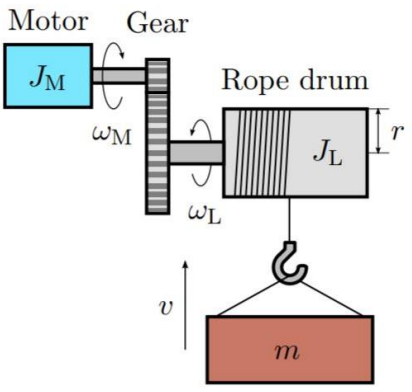
\includegraphics[width=0.4\textwidth]{assets/hoistoefening.png}
  \caption{Hoist Oefening}
  \label{fig:hoistoefening.png}
 \end{figure}
Volgende waardes zijn gegeven:
\begin{itemize}
    \item \textbf{m = 650 kg} $\rightarrow F_{load} = m \cdot g = 650 kg \cdot 9.81 m/s^2 = 6376.5 N$
    \item $\mathbf{h_{hoist} = 13 m}$
    \item $\mathbf{t_{hoist} = 30 s}$ 
    \newline
    Samen met de hoogte vinden we de arbeid geleverd door de last en dus het nodige vermogen met deze tijd: $W = F_{load} \cdot h_{hoist} = 6376.5 N \cdot 13 m = 82894.5 J$ en $P_{mass} = \frac{W}{t_{hoist}} = \frac{82894.5 J}{30 s} = 2763.15 W = 2.76 kW$ Ook vinden we de snelheid van de last: $v_{mass} = \frac{h_{hoist}}{t_{hoist}} = \frac{13 m}{30 s} = 0.433 m/s$
    \item $\mathbf{d_{drum} = 70 cm}$ 
    \newline
    Hiermee vinden we het koppel op de rol: $T_{drum} = F_{load} \cdot \frac{d_{drum}}{2} = 6376.5 N \cdot \frac{0.7 m}{2} = 2231.78 Nm$
    \item $\mathbf{l_{drum} = 4 m}$
    \item $\mathbf{\rho_{steel} = 7800\ kg/m^3}$
\end{itemize}
Met de snelheid van de massa kunnen we ook het toerensnelheid van die rol (drum) bepalen:
\begin{align*}
    n_{drum} = \frac{v_{mass}}{\pi \cdot d_{drum}} \cdot 60 = \frac{0.433 m/s}{\pi \cdot 0.7 m} \cdot 60 = 11.8 rpm (\omega_{drum} = \omega_{L} = 1.23 rad/s)
\end{align*}
Er wordt hier geen poolpaartal ofzo gegeven of berekend, ik denk dus dat het is dat je in deze toepassing zowieso moet kiezen uit een 4 polige motor uit een catalogus die ik zometeen ga tonen, deze motors hebben dus 4 polen en dus een nominale snelheid tussen de 1400rpm en 1500rpm, op voorand weet je dit niet altijd exact want je kiest nog geen motor. We hebben hier dus wel al zowieso een overbrenging nodig want onze drum draait veel trager dan de motor. We gaan een gemiddelde nemen van 1450 rpm om de overbrengingsverhouding te bepalen:
\begin{align*}
  i = \frac{n_{mot}}{n_{drum}} = \frac{1450 rpm}{11.8 rpm} = 122.88
\end{align*}
Bij deze oefening gaan we van een rendement van 0.7 uit dus gaat een 3kW motor niet voldoende zijn, we berekenen een vermogen voor de motor van:
\begin{align*}
    P_{mot} = \frac{P_{mass}}{\eta} = \frac{2.76 kW}{0.7} = 3.94 kW
\end{align*}
Dus kiezen we een 4kW motor uit de catalogus, deze heeft wel 1443 tr/min en een rendement op vollast van 0.886 dus eigelijk moet je iteraties doen hiermee en dus opnieuw berekenen.
\begin{figure}[H]
  \centering
  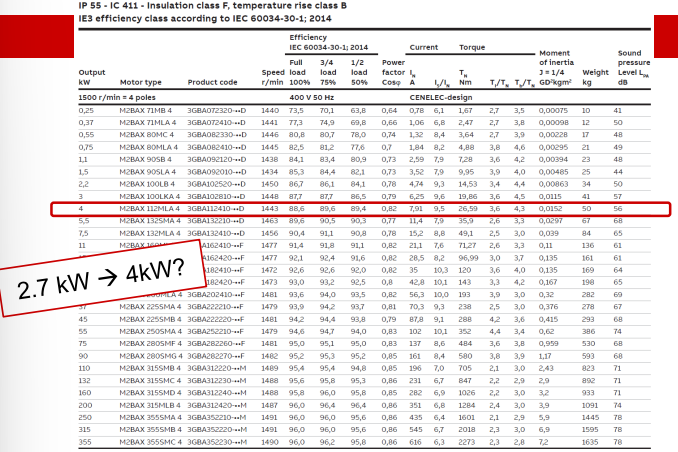
\includegraphics[width=0.6\textwidth]{assets/motorcatalogushoist.png}
  \caption{Motor Catalogus Hoist}
  \label{fig:motorcatalogushoist.png}
 \end{figure}
Maar 1 ding waar we nog geen rekening mee hebben gehouden is dat het hijstoestel niet onmiddelijk op topsnelheid start en niet onmiddelijk stopt, het versnelt eerst, houdt een tijdje de topsnelheid aan en vertraagt weer zoals we zien in volgende figuur:
\begin{figure}[H]
  \centering
  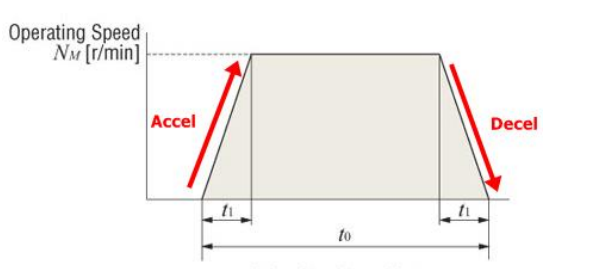
\includegraphics[width=0.6\textwidth]{assets/trapzeiumvormsnelheid.png}
  \caption{Trapzeiumvormige snelheid van de last bij een hijstoestel}
  \label{fig:trapzeiumvormsnelheid.png}
 \end{figure}
Die tijd om te versnellen en te vertragen is eigelijk niet meegegeven in onze opgave (deze wordt bijna nooit meegegeven zelfs), in de praktijk nemen we dan zelf een realistische waarde aan zoals $t_{acc} = t_{dec} = 2 s$. Tijdens deze tijd legt de last wel minder afstand af dan bij die topsnelheid, dus om 13 m in 30s te halen gaat onze snelheid iets hoger moeten liggen dan de eerder berekende snelheid. Als we zeggen dat onze beide driehoeken van die trapezium evenveel afstand afleggen als 1 rechthoekige blok in dus die 2s (niet 4!) aan de topsnelheid dan kunnen we de juiste topsnelheid berekenen met:
\begin{align*}
 v_{top} = \frac{h_{hoist}}{t_{hoist} - t_{acc}} = \frac{13 m}{30 s - 2 s} = 0.464 m/s
\end{align*}
Met deze snelheid berekenen we het statisch (niet-versnellende) vermogen (rekening houden met dat rendement terug):
\begin{align*}
 P_{stat} = \frac{F_{load} \cdot v_{top}}{\eta} = \frac{6376.5 N \cdot 0.464 m/s}{0.7} = 4.23 kW
\end{align*}
Dit is dus eigelijk een deel van ons totaal vermogen dat we nodig hebben, we hebben namelijk ook nog een dynamisch vermogen nodig om de massa te versnellen. Dit vermogen dient vooral om alle traagheidsmomenten van het systeem te versnellen, deze hebben eigelijk een bepaald koppel nodig:
\begin{align*}
 T_{dyn} = J \cdot \alpha
\end{align*}
Al deze relevante traagheidsmomenten van de verschillende massas dus gaan wel gereflecteerd/transformeerd moeten worden (geherleid) naar de motoras, dit wordt normaal gedaan met de volgende formule:
\begin{align*}
 J_{x} = \frac{J_{load}}{i^2}
\end{align*}
Maar voor een lineair bewegende massa zoals hier is er een andere formule die we kunnen gebruiken, namelijk:
\begin{align*}
    J_{x} = \frac{m \cdot v^2}{\omega^2}
\end{align*}
In ons geval hebben we drie bijdragen:
\begin{itemize}
 \item $\mathbf{J_{rotor}}$: Het traagheidsmoment van de motor zelf, deze kunnen we aflezen uit de motorcatalogus en bedraagt hier dus 0,0152 $kg m^2$
 \item $\mathbf{J_{drum}}$: Het traagheidsmoment van de rol, bij benadering is dit een volle stalen cillinder met de gegeven $\rho_{Steel}$, $r_{drum}$ en $l_{drum}$, dit traagheidsmoment wordt berekend met:
 \begin{align*}
 J_{drum} = \frac{1}{2} \cdot m_{drum} \cdot r_{drum}^2
 \end{align*}
  Met $m_{drum} = \rho_{steel} \cdot \pi \cdot r_{drum}^2 \cdot l_{drum}$. Die formule voor de cilinder komt uit deze tabel:
  \begin{figure}[H]
    \centering
    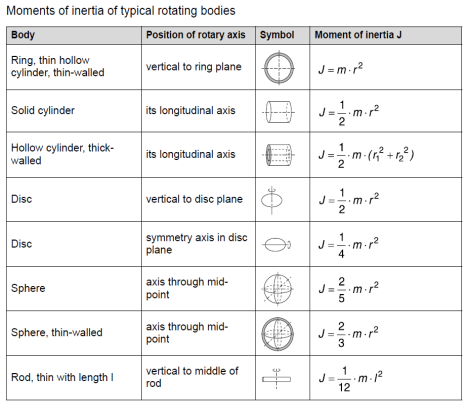
\includegraphics[width=0.4\textwidth]{assets/traagheidsmomenten.png}
    \caption{Tabel traagheidsmomenten van verschillende vormen}
    \label{fig:traagheidsmomenten.png}
   \end{figure}
 \item $\mathbf{J_{massa}}$: Het traagheidsmoment van de massa, dit is herleid naar de as van de drum (rol) en wordt berekend met:
    \begin{align*}
    J_{massa} = \frac{m_{massa} \cdot v_{top}^2}{\omega_{drum}^2} = m_{massa} \cdot r_{drum}^2 
    \end{align*}
    (Want $v_{top} = \omega_{drum} \cdot r_{drum}$)
\end{itemize}
Het optellen van deze traagheidsmomenten + het herleiden naar de motoras voor het traagheidsmoment van de drum en de massa (rekening houdend met een rendement $\eta_{GB}$ van de tandwielkast) wordt dan als volgt gedaan:
\begin{align*}
    J_{tot} = J_{rotor} + \frac{J_{drum} + J_{massa}}{i^2 \cdot \eta_{GB}} = 0.105 kg m^2
\end{align*}
(Dat rendement is niet gegeven in deze oefening, gewoon de uitkomst van $J_{tot}$ staat op de slides, op toledo staat er wel een gearbox efficiency van 90\% bij dezelfde oefening als deze met iets andere gegevens)
\newline
\newline
De hoekversnelling van de motor $\alpha$ kunnen we berekenen met de volgende formule:
\begin{align*}
    \alpha = \omega_{top}/t_{acc} = 151.5 rad/s / 2 s = 75.8 rad/s^2
\end{align*}
Hiermee kunnen we dan het dynamisch koppel berekenen:
\begin{align*}
    T_{dyn} = J_{tot} \cdot \alpha = 0.105 kg m^2 \cdot 75.8 rad/s^2 = 7.96 Nm
\end{align*}
Het dynamisch vermogen dat we nodig hebben om de massa te versnellen is dan:
\begin{align*}
    P_{dyn} = T_{dyn} \cdot \omega_{top} = 7.96 Nm \cdot 151.5 rad/s = 1.21 kW
\end{align*}
Het werd wel niet verder uitgelegd op de slide maar dit resultaat is een eerste ruwere doorrekening, na een iteratie is er gevonden voor dit vermogen dat het gelijk is aan 1.37 kW waardoor het optellen een totaal vermogen geeft van:
\begin{align*}
    P_{tot} = P_{stat} + P_{dyn} = 4.23 kW + 1.37 kW = 5.6 kW
\end{align*}
Dus een totaal koppel van:
\begin{align*}
    T_{tot} = \frac{P_{tot}}{\omega_{top}} = \frac{5.6 kW}{151.5 rad/s} = 36.6 Nm
\end{align*}
Uit de catalogus kiezen we nu echter voor een 5.5 kW motor, ons totaal koppel hierbij is wel iets hoger dan ons nominaal koppel maar dat boeit niet want het kipkoppel is 2,6 keer groter.
\begin{figure}[H]
  \centering
  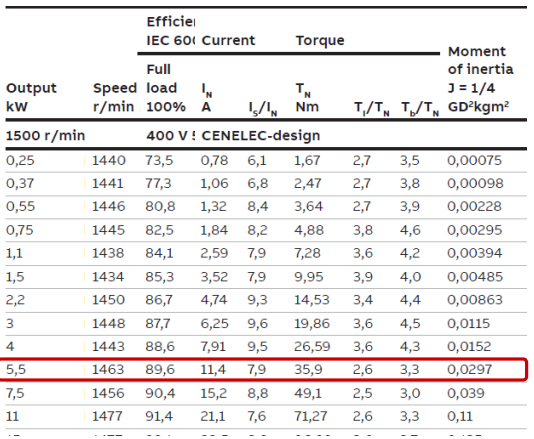
\includegraphics[width=0.5\textwidth]{assets/55kwmotorselectie.png}
  \caption{Motorcatalogus 5.5 kW motor}
  \label{fig:55kwmotorselectie.png}
 \end{figure}
\begin{warningbox}[5.5 kW motor terwijl we 5.6 kW nodig hebben?]
 Hoewel ons totaal vermogen berekend is op 5.6 kW, kiezen we toch een 5.5 kW motor uit de catalogus, dit is het nominaal vermogen, het is niet erg om hier even over te zitten (zoals dus tijdens die 2 seconden bij ons), we kunnen dit dus wel even overbelasten. Dit is een betere keuze dan een overgedimensioneerde motor te kiezen. Je moet dus ook controleren of die motor de korte piekbelasting van 36.6 Nm in ons geval aankan zonder continu op dat niveau te moeten draaien, wat het dus kan hier want de aanloop-/piekkoppel t.o.v. nominaal koppel verhouding is 2.6
\end{warningbox}
% ==================================================================
\newpage
\chapter{Kleine Motoren/Machines (Small Motors)}
Nu gaan we kijken naar een paar speciale types motoren, vooral toepassingen van de motoren die we tot nu toe gezien hebben. De verschillende motoren waarover we het gaan hebben zijn de volgende:
\begin{itemize}
    \item 1-fasige motoren (deze vind je vooral thuis in apparaten zoals wasmachines, stofzuigers, $\cdots$)
    \begin{itemize}
     \item Universeel motoren
     \item 1-fasige inductie motor (Gewone 1f inductiemotor, Condensator motor, Spleetpool motor)
    \end{itemize}
    \item Vermogen elektronica gestuurde motoren
    \begin{itemize}
        \item BLDC (vooral de deze is belangrijk)
        \item Reluctantie motoren
        \item Stepper motoren
    \end{itemize}
\end{itemize}
\section{Universeel motor}
Universeel motors zijn \textbf{DC-seriemotoren} die werken op zowel AC als DC (1-fasig), dit is waarom we het zoveel in huishoudtoestellen vinden, het zijn eigelijk variaties van een DC-machine. Een motor die dus zowel op een batterij (DC) als op het stopcontact (AC) werkt. Maar hoe werkt dit? Daarvoor gaan we even terug naar de vergelijkingen voor een DC-machine:
\begin{align*}
 E = k \cdot \varphi \cdot \omega = G \cdot I_e \cdot \omega \\
 T = k \cdot \varphi \cdot I_a = G \cdot I_e \cdot I_a
\end{align*}
\begin{figure}[H]
  \centering
  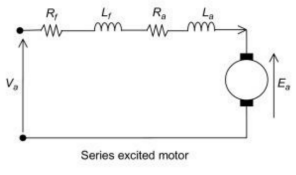
\includegraphics[width=0.5\textwidth]{assets/dcserieschakelele.png}
  \caption{Herhaling DC-serie schakeling}
  \label{fig:dcserieschakelele.png}
 \end{figure}
Uit de DC-serie schakeling weten we ook dat $I_e = I_a = I$, bij een shun bekrachtiging worden deze stromen apart aangestuurd, als je dat dan op AC aansluit dan wisselt het statorveld steeds van polariteit. Als de ankerstroom daar niet perfect synchroon mee wissel, keert op sommige momenten of het veld of de stroom van teken, nooit beide, en dan wordt het koppel $T = G \cdot I_e \cdot I_a$ altijd negatief en het resulterende gemiddelde koppel over een periode wordt zo goed als nul. Conclusie: bij een shunt bekrachtiging gaat AC de motor niet doen draaien, alleen een beetje trillen. Bij een serie bekrachtiging is dit anders, want de stroom door de ankerwikkeling en de veldwikkeling is dezelfde, dus als het veld van teken wisselt dan wisselt de ankerstroom ook van teken en blijft het koppel $T = G \cdot I_e \cdot I_a$ altijd positief. Het resulterende gemiddelde koppel over een periode is dus niet nul en de motor draait gewoon verder. Dit is dus waarom een DC-serie motor op AC kan werken. Kan je ook zien aan het feit dat $T = G \cdot I^2$ een kwadraat heeft (altijd positief).
\begin{figure}[H]
  \centering
  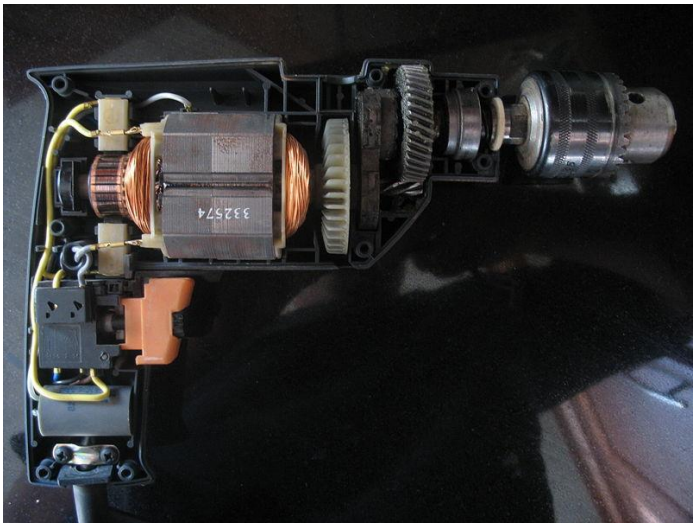
\includegraphics[width=0.5\textwidth]{assets/voorbeeldbooruniverseelmotor.png}
  \caption{Voorbeeld van een universele motor}
  \label{fig:voorbeeldbooruniverseelmotor.png}
 \end{figure}
In de figuur een voorbeeld van een universele motor in een boor, je kan hier duidelijk de commutator zien.
\newline
\newline
Dit hebben we eigelijk al eerder gezien, maar hier wordt het rap herhaald maar als we de inwendige spanning invullen in de spanningsvergelijking kunnen we omvormen naar de stroom en dit invullen in de koppel formule om een vergelijking van het koppel toerental karakteristiek te bekomen:
\begin{align*}
 U_a = E + R_a \cdot I = G \cdot I \cdot \omega + R_a \cdot I \\
\Rightarrow I = \frac{U_a}{G \cdot \omega + R_a} \\
\Rightarrow T = G \cdot I^2 = G \cdot \left(\frac{U_a}{G \cdot \omega + R_a}\right)^2
\end{align*}
Dit vormt dus de eerder geziene hyperbole T-n karakteristiek:
\begin{figure}[H]
  \centering
  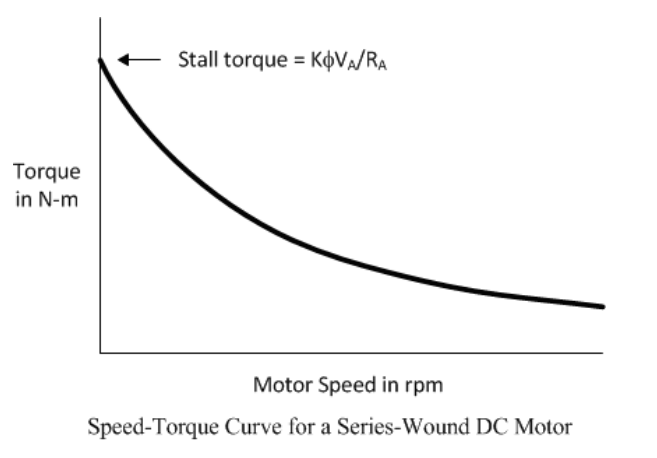
\includegraphics[width=0.5\textwidth]{assets/TNseriemootr.png}
  \caption{T-n karakteristiek van een DC-serie motor}
  \label{fig:TNseriemootr.png}
 \end{figure}
\subsection{Nadelen van een universele motor}
({\color{red}Deels door AI gecooked hier, maar het klopt allemaal})
\newline
En dan komen we nu ook terug op 1 van die grote nadelen dat al besproken was, namelijk dat als je koppel naar 0 gaat, de snelheid naar oneindig gaat (wat we ook op onze karakteristiek zien). Wat het extra gevaarlijk hier maakt is het feit dat als de stroom daalt (dat trouwens ook evenredig is aan het veld) dat het koppel hard daalt (kwadratisch) en dus ook het veld, en om $E \approx V_\phi$ te houden moet de snelheid dan stijgen omdat ons veld zo zwak is. Dit heet dus \textbf{'op hol slaan'} en is in theoretisch naar oneindig maar in het echt zijn er verliezen enzo dus gaat dit gewoon heel hoog worden.
\newline
\newline
Een ander nadeel is dat als de motor stil staat dat er een heel grote stroom door de wikkelingen gaat (want $E = 0$ dus $I = \frac{U}{R}$) en dit kan de wikkelingen doen verbranden zeker als de rotor geblokkeerd is, bvb als je boor vast zit. Meestal is er wel een soort van zekering voorzien.
\newline
\newline
Een volgend nadeel is dat het koppel \textbf{pulseert}. Bij een zuivere DC-seriemotor is de stroom constant, dus is het koppel dat ook. Bij de universele motor (op AC) is de stroom sinusvormig, en aangezien $T = G \cdot I^2$, is het koppel dus een gekwadrateerde sinus, het blijft wel altijd positief (want een kwadraat), maar het is niet meer vlak, het pulseert tussen 0 en een piekwaarde aan het dubbele van de netfrequentie. Dat geeft trillingen en geluid, en is meteen ook de reden waarom je een universele motor bijna uitsluitend thuis tegenkomt (boormachine, mixer, stofzuiger) en niet in de industrie, waar je meestal een vlakkere, trillingsvrije aandrijving wil.
\begin{figure}[H]
  \centering
  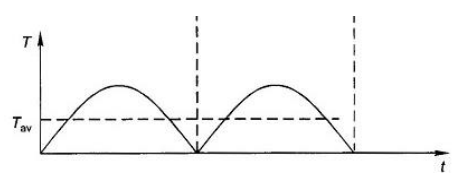
\includegraphics[width=0.6\textwidth]{assets/pulserendkoppel.png}
  \caption{Pulserend koppel van een universele motor op AC}
  \label{fig:pulserendkoppel.png}
 \end{figure}
Er zijn ook extra \textbf{ijzerverliezen} door de statorconstructie. Bij een zuivere DC-motor is het statorveld constant, dus is er geen hysteresis- of wervelstroomverlies in het statorijzer, en volstaat een massieve (niet-gelamelleerde) statorkern. Bij AC wisselt het statorveld wel voortdurend mee met de netfrequentie, wat in een massieve kern net wel hysteresis- en wervelstroomverliezen zou geven. Daarom moet de stator van een universele motor, net zoals de rotor, ook \textbf{gelamelleerd} gebouwd worden, wat extra kost en complexiteit met zich meebrengt die een zuivere DC-seriemotor niet heeft. (De rotor is trouwens sowieso altijd gelamelleerd, ook bij DC, want vanuit een rotorgeleider gezien wisselt het veld toch, aangezien die geleider om beurten een noord- en een zuidpool voorbij ziet komen terwijl hij ronddraait.)
\newline
\newline
Een gerelateerd nadeel is de grotere invloed van de \textbf{terug-emk (back-emf)}. De volledige spanningsvergelijking is:
\begin{align*}
 U_a = E + R_a I_a + L_a \frac{di_a}{dt}.
\end{align*}
Bij DC in stationair regime is $\frac{di_a}{dt}=0$, dus die term valt weg. Bij AC verandert de stroom voortdurend, dus dat spanningsvalletje over de inductantie is er altijd bij en 'eet' een deel van $U_a$ op. Er blijft dan minder spanning over voor $E$, en aangezien $E = C\varphi\omega = G \cdot I \cdot \omega$, betekent minder $E$ bij dezelfde stroom een lagere snelheid voor dezelfde effectieve voedingsspanning. De universele (AC-)versie draait dus trager dan de zuivere DC-versie bij gelijke spanning en belasting.
\newline
\newline
Dit wordt ook mooi bevestigd op de koppel-snelheidsgrafiek: bij eenzelfde percentage van het vollastkoppel ligt de snelheidscurve voor DC-voeding hoger dan die voor AC-voeding. Met andere woorden: dezelfde motor presteert altijd net iets beter op DC dan op AC, precies door de extra ijzer- en inductieverliezen hierboven.
\newline
\newline
Een laatste ding dat we ook nog kunnen zien in volgende figuur is dat we een iets lager koppel hebben als we de universele motor op AC aansluiten:
\begin{figure}[H]
  \centering
  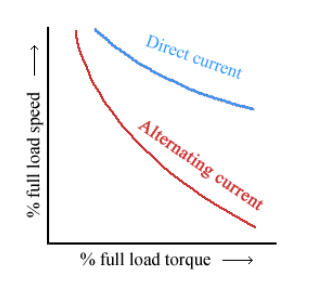
\includegraphics[width=0.4\textwidth]{assets/ACDCTN.png}
  \caption{AC vs DC T-n karakteristiek van een universele motor}
  \label{fig:ACDCTN.png}
 \end{figure}
\section{1-fasige inductie motor}
Dan kijken we nu naar de andere éénfasige motor, de 1-fasige inductie motor. Net zoals de universele motor mag deze motor op het stopcontact. Voor opbouw berschilt deze niet te veel van de normale inductiemotor, hij heeft ook een \textbf{kooirotor} die eigelijk exact hetzelfde is. Het is bij de stator dat er wat verschil is want hier hebben we namelijk \textbf{1 statorwikkeling} (want we kunnen maar 1 fase aansluiten). Ook heeft deze motor een \textbf{centrifugaal schakelaar}, dit is een mechanische schakelaar die reageert op de rotatiesnelheid, hij schakelt om zodra de rotor een bepaalde snelheid bereikt (Het nut hiervan zien we zometeen).
\begin{figure}[H]
  \centering
  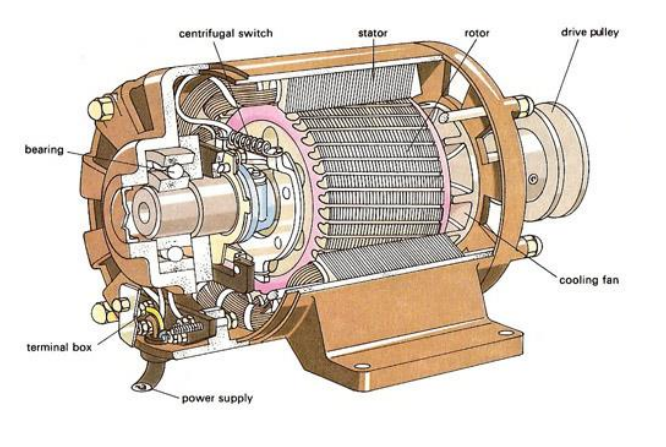
\includegraphics[width=0.5\textwidth]{assets/eenfasigeinductiemachine.png}
  \caption{Eénfasige inductiemachine}
  \label{fig:eenfasigeinductiemachine.png}
 \end{figure}
De koppel-toerental karakteristiek van deze motor ziet er als volgt uit (het is die Single-phase op de figuur):
\begin{figure}[H]
  \centering
  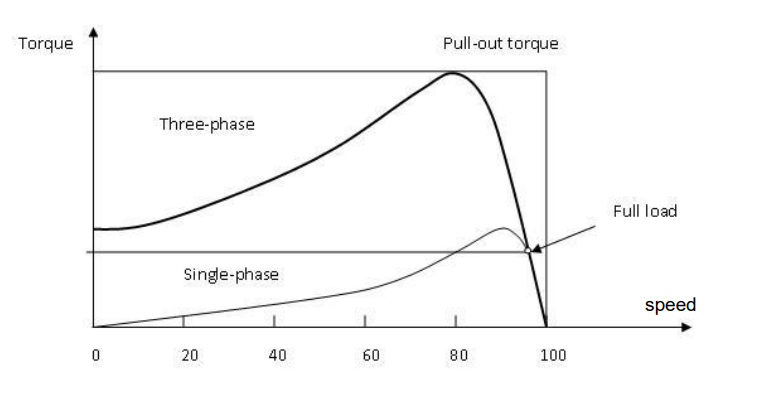
\includegraphics[width=0.6\textwidth]{assets/TNeenfasigeim.png}
  \caption{Koppel-toerental karakteristiek van een éénfasige inductiemachine}
  \label{fig:TNeenfasigeim.png}
 \end{figure}
Hier op zien we een probleem, namelijk dat bij de 1-fasige inductiemachine er \textbf{geen startkoppel} is, dit omdat een stator met maar 1 wikkeling enkel een wisselveld geeft, er is geen draaiveld. Dit wisselveld induceert wel spanning/stroom in de rotorstaven maar zoals de grafiek toont is het koppel 0 op n = 0 dus kan het niet starten. De motor heeft dus wel een soort synchrone snelheid waarbij het koppel nul wordt zoals bij de normale inductiemotor. \textit{Van zodra de 1-fasige inductiemotor draait levert hij wel koppel.}
\subsection{Werking van de 1-fasige inductiemachine}
Hoezo heeft een wisselveld nog koppel eigelijk? We gaan het als volgt bekijken, we hebben in de volgende figuur ons wissledveld, dit kan beschreven worden als een staande golf (hier in het zwart). Ook kan dit puur pulserend veld beschreven worden als de som van \textbf{twee even grote velden die met dezelfde snelheid in tegengestelde richting ronddraaien}. Op de figuur is dit de paarse curve (een som van een blauwe en rode curve in tegengestelde richting):
\begin{figure}[H]
  \centering
  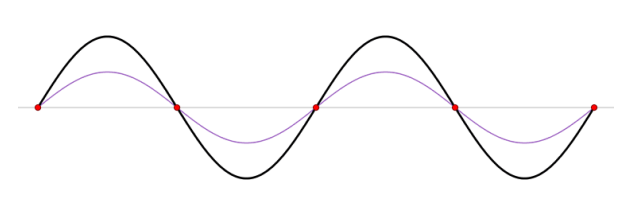
\includegraphics[width=0.8\textwidth]{assets/veld1fasigeIM.png}
  \caption{Curve van het wisselend statorveld van een 1-fasige inductiemachine}
  \label{fig:veld1fasigeIM.png}
 \end{figure}
Om dit duidelijker te maken zien we in volgende figuur de 2 fasoren van die tegengestelde velden, ze draaien in tegengestelde richting en op elk punt als je die 2 fasoren optelt gaan die dus die paarse curve vormen:
\begin{figure}[H]
  \centering
  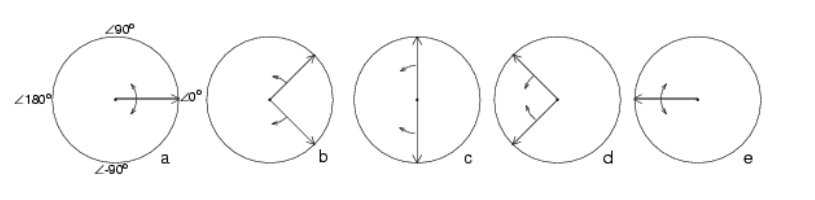
\includegraphics[width=0.8\textwidth]{assets/fasorenblauwenroodveld.png}
  \caption{Fasoren van de tegengestelde velden}
  \label{fig:fasorenblauwenroodveld.png}
 \end{figure}
Nu wat zijn we hiermee? Dat we weten dat dit zo kan beschreven worden? Awel, sinds dat dit 2 aparte fictieve draaivelden zijn kunnen die zich ook gedragen als draaivelden van een gewone inductiemotor en genereren die dus elk een eigen koppel-slip-curve die we in de volgende figuur met de stippenlijnen zien:
\begin{figure}[H]
  \centering
  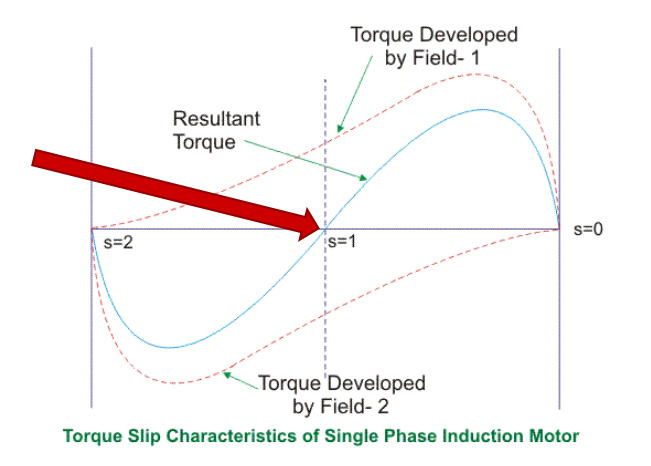
\includegraphics[width=0.8\textwidth]{assets/singlephadetorquetheoreticalapproach.png}
  \caption{1 fasige inductiemachine koppel theoretische benadering}
  \label{fig:singlephadetorquetheoreticalapproach.png}
 \end{figure}
De bovenste rode stippenlijn is dan voor dat rode draaiveld en de onderste rode stippelijn is dan voor dat blauwe draaiveld (ik weet dat het confusing is dat beide stippelijnen rood zijn en de vollelijn in het midden blauw $\#$shitfiguur). Bij stilstand heeft de rotor exact dezelfde slip tegenover deze beide velden (ze draaien evensnel in tegengestelde richting, dus evensnel tegengestelde koppels $\rightarrow T_{res} = 0$). Zodra de rotor een duwtje krijgt (bvb. voorwaarts), wordt de slip tegenover het voorwaartse veld kleinen, dus veel koppel en de slip van het achterwaartse veld groter, dus minder koppel. Het netto koppel wordt dan positief (in de richting dat je hem duwde) en de motor versnelt!
\newline
\newline
({\color{red}Volgende uitleg snap ik zelf niks van, AI kon het mij ook niet deftig uitleggen, ik heb deze uitleg uit een samenvatting gevonden})
\newline
\textit{Een andere manier om deze werking te verklaren is een meer fysisch perspectief. Voor de fysische betekenis van dit koppel gaan we kijken naar de figuur hier onder. We hebben namelijk een rotor die ronddraait. De stator heeft dan een wisselend magnetisch veld, waardoor in hetzelfde vlak een spanning wordt geïnduceerd. Dit is dus nog steeds hetzelfde als bij stilstand. Maar omdat de rotor draait, en de rotor inductief is, gaat de stroom pas ontstaan als de motor al gedraaid is. Hierdoor gaan we dus ook een magnetisch veld opwekken in de rotor, wat staat volgens de lijn van de maximale stroom. Hierdoor gaat er dus ook een koppel ontstaan bij een motor. }
\begin{figure}[H]
  \centering
  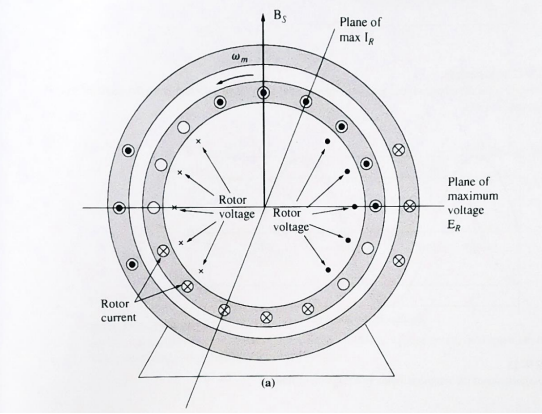
\includegraphics[width=0.4\textwidth]{assets/crossfieldtheory.png}
  \caption{Fysische betekenis (cross field theory)}
  \label{fig:crossfieldtheory.png}
 \end{figure}
(De uitleg die ik ervan heb verstaan in de les is dat als je op de rotor staat en deze in beweging is (draait), dan zie je niet overal een even sterk veld want de stator is 1 wisselveld, dus ga je op sommige plaatsen in de rotor grotere stromen gaan hebben wat voor een netto koppel zorgt (als de motor toch in bewegin is) en de motor gedraagt zich hier dan inductief)
\subsection{Starten van een 1-fasige inductiemachine}
Nu gaan we dan kijken naar hoe we zo een 1-fasige machine kunnen starten aangezien ze geen startkoppel hebben. Hier zijn verschillende manieren voor, maar natuurlijk moet je ook in rekening houden dat dit kleine machines zijn, dus ze aandrijven met een andere grote hulpmotor gaat niet lukken (een kleine wel misschien).
\newline
\newline
Het makkelijkste dat we kunnen doen is hem natuurlijk manueel/extern aanduwen, gewoon een klein duwtje geven en hij draait. \textit{(Of zoals Prof. Nobels het zei: 'We laten een chineesje de motor aanlopen!')}. De andere manier om de motor te starten is met een \textbf{hulpwikkeling}, dit is een 2de wikkeling die $90^\circ$ verschoven is tegenover die éne statorwikkeling zoals in volgende figuur:
\begin{figure}[H]
  \centering
  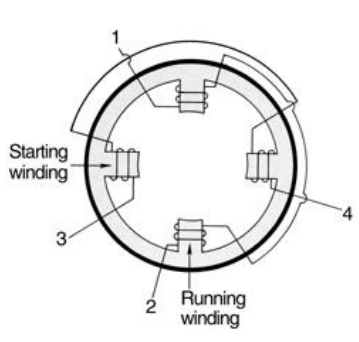
\includegraphics[width=0.4\textwidth]{assets/hulpwikkeling.png}
  \caption{Starting winding is die hulpwikkeling, de andere is de hoofdwikkeling}
  \label{fig:hulpwikkeling.png}
 \end{figure}
We doen dit want samen kunnen 2 wikkelingen wel een (bij benadering) draaiveld opwekken, ideaal is dit dus natuurlijk een mooi rond draaiveld maar omdat beide wikkelingen hier op dezelfde ééncontactspanning hangen (en we dus geen tweede fase eigelijk hebben) gaan we deze hulpwikkeling elektrisch iets anders moeten bouwen dan de hoofdwikkeling (bvb. dunnere draad, meer weerstand, minder inductief) zodat de stroom van nature een beetje voorloopt tegenover de stroom in de (meer inductieve) hoofdwikkeling. Zo hebben we wel een faseverschil en gaan we een draaiveld krijgen, dit draaiveld gaat nooit exact $90^\circ$ zijn maar eerder een \textbf{elliptisch draaiveld} maar dit is nog steeds sterk genoeg om de motor aan te lopen. En hier is dan het speciale! Eens dat de motor op snelheid is gekomen schakelt die \textbf{centrifugaal schakelaar} de hulpwikkeling automatisch uit want die hulpwikkeling kan anders doorbranden en zowieso ook voor te veel verliezen zorgen. Wat we wel kunnen doen om dichter bij die $90^\circ$ te geraken is een condensator in serie met de hulpwikkeling zetten, zo duw je eigelijk dat faseverschil dichter naar $90^\circ$. Hierdoor kan je een hoger opstartkoppel bereiken. Dit noemt dan eigelijk de \textbf{condensator motor}, we kunnen deze ook tijdens het normaal bedrijf van de motor verder laten draaien met nog een aparte kleinere condensator wat net iets beter is of gewoon gebruiken enkel tijdens het opstarten en dan uitschakelen met de centrifugaal en het verschil tussen de koppeltoerental karakteristiek van de deze (met dus hulpwikkeling met condensator en de gewone motor met de hoofdwikkeling) ziet er dan zo uit:
\begin{figure}[H]
  \centering
  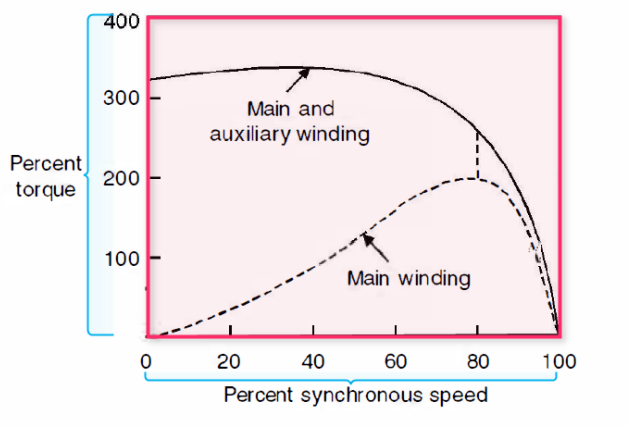
\includegraphics[width=0.5\textwidth]{assets/TNcondensatormotor.png}
  \caption{T-n karakteristiek van een condensator motor (met hulpwikkeling) vs gewone 1-fasige inductiemotor}
  \label{fig:TNcondensatormotor.png}
 \end{figure}
De condensator motor wordt ook wel de beste 1-fasige motor genoemd. De eer van de slechtste 1-fasige motor gaat naar de spleetpoolmotor.
\subsubsection{Spleetpoolmotor}
Dit is wel echt een heel kleine motor en heeft eigelijk meer als nut ook het starten van de 1-fasige inductie-motor, het is dus niet echt een aparte variant van die motor, dit dient vooral voor kleine vermogen met lage efficiënties. Het is dus ook de goedkoopste/eenvoudigste manier om een 1-fasige inductiemotor te laten starten (maar dus ook de slechtste). Het idee is hier dat je geen aparte hulpwikkeling in deze kleine motor gebruikt maar dat je met de hoofdwikkeling zelf hier 4 polen maakt en dat die polen eigelijk gesplitst zijn fysiek. Rond een deel van elk van die gesplitste polen wordt een kortgesloten koper ringetje geplaatst (dus niet enkel op 1 pool, maar op elke pool, telkens aan dezelfde kant) waardoor er daarin telkens een stroom wordt geïnduceerd door het feit dat de flux van de hoofdwikkeling daar pulseert. Wat dit doet is dan de verandering tegenwerking waardoor de flux in dat klein stukje vertraagd wordt en er dus een soort van faseverschil ontstaat waardoor er een klein koppel ontstaat. Het statorveld wordt trouwens apart opgewekt en zo naar de rotor gebracht. Je ziet dit in volgende figuur (die stator zijn de oranje wikkelingen, het veld wordt via dat gelamelleerd ijzer verder gebracht):
\begin{figure}[H]
  \centering
  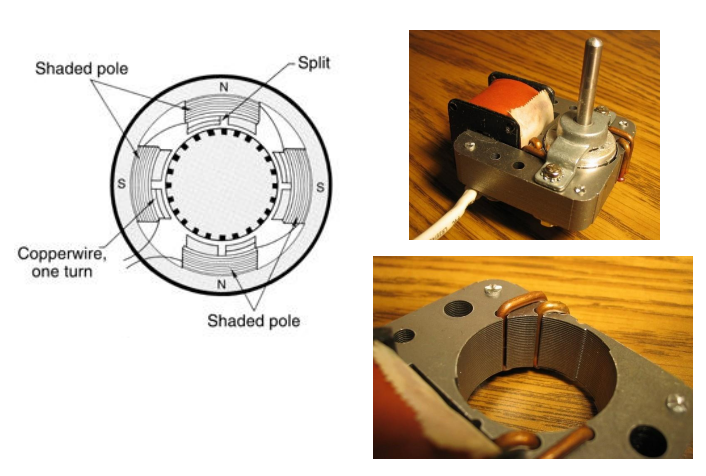
\includegraphics[width=0.6\textwidth]{assets/spleetpoolmotor.png}
  \caption{Spleetpoolmotor}
  \label{fig:spleetpoolmotor.png}
 \end{figure}
\subsection{Koppel-Toerental karakteristieken van de 1-fasige inductiemotoren}
De volgende grafiek toont alle besproken startmethodes naast elkaar van beste naar slechtste koppel:
\begin{figure}[H]
  \centering
  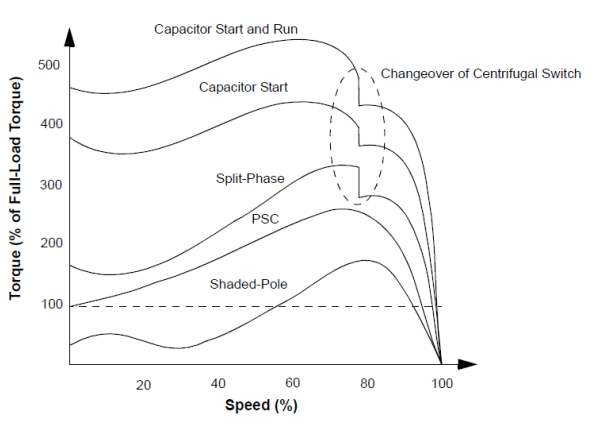
\includegraphics[width=0.6\textwidth]{assets/Tnkarakteritstieken1fmotore.png}
  \caption{Koppel-Toerental karakteristieken van de 1-fasige inductiemotoren}
  \label{fig:Tnkarakteritstieken1fmotore.png}
 \end{figure}
De 'Split-phase' motor is de gewone 1-fasige inductiemotor met hulpwikkeling trouwens, de PSC (Permanent Split Capacitor) is condensator + hulpwikkeling zonder een schakelaar, capacitator start en run heeft een kleine runcondensator nog en capacitator start is gewoon de grotere normale condensator helemaal los (had nooit zo een run condensator) en shaded pole is dus de spleetpoolmotor, je ziet dat deze ook gekke effecten heeft en dus een slecht rendement.
\newline
\newline
En in volgende tabel zien we nog rap een kort overzicht van de 5 verschillende 1-fasige motors:
\begin{figure}[H]
  \centering
  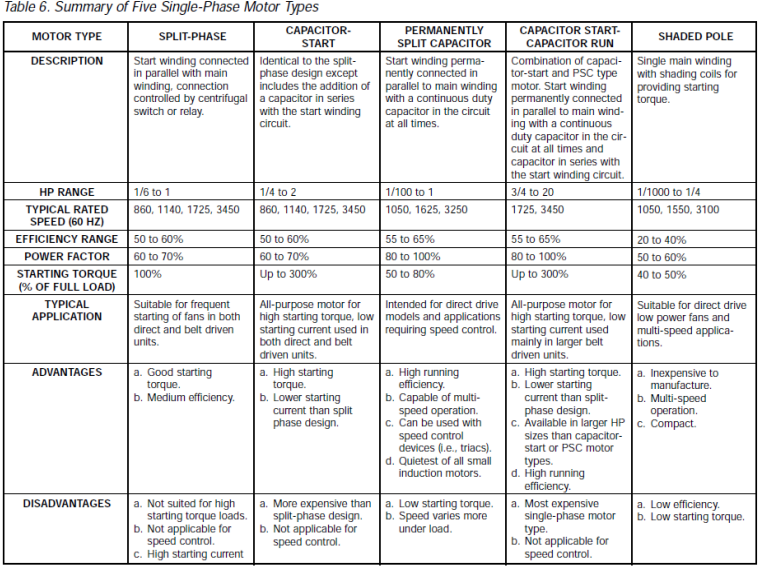
\includegraphics[width=0.6\textwidth]{assets/tabel1fmotors.png}
  \caption{Tabel van de 5 verschillende 1-fasige inductiemotoren}
  \label{fig:tabel1fmotors.png}
 \end{figure}
We zien dat de 'permanently split capacitator' en 'capacitator start capacitator run' motoren het beste rendement hebben.
\section{BLDC (Brushless DC) motor}
Dan gaan we nu over naar de vermogenelektronica gestuurde motoren, we gaan eigelijk vooral de deze bespreken. De BLDC is elektrisch gezien een DC machine maar dan \textit{zonder een mechanische commutator en borstels}. Wat hier ook belangrijk is, is dat\textbf{ het anker hier de stator is en de bekrachtiging de rotor!} Dit was omgekeerd bij de normale DC-machine!!! De wikkelingen zitten bij de BLDC dus vast op de stator en draaien de permanente magneten mee met de rotor (zelfde opbouw als de permanentmagneet synchroonmachine). Doordat er geen borstels zijn \textit{kan de BLDC niet rechtstreeks op een batterij (of stopcontact) aangesloten worden}, we hebben hier dus altijd een elektronische controller nodig die de stroom naar de juiste wikkeling op het juiste moment stuurt. Hier is voor de zekerheid en verduidelijk nog een tabel waarin staat wat het anker en wat de bekrachtiging is bij de (PM)DC, BLDC en (PM)SM:
\begin{figure}[H]
  \centering
  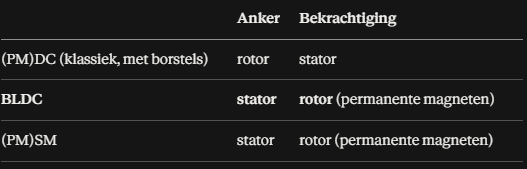
\includegraphics[width=0.6\textwidth]{assets/tabelmachinesankerbekrachtiging.png}
  \caption{Tabel van de anker- en bekrachtigingswikkelingen van de verschillende machines}
  \label{fig:tabelmachinesankerbekrachtiging.png}
 \end{figure}
\subsection{Werking van de BLDC motor}
Dus bij de BLDC heb je niet de commutator met borstels dat als mechanische inverter werkt en ervoor zorgt dat de stroom door de rotors steeds in de juiste richting staat, hier ga je het dus moeten doen met elektronica. Om te weten wanneer er precies moet geschakeld worden moet de controller dus weten waar de rotor zich precies bevindt. Dit gebeurt met \textbf{Hall-sensoren}, door er zo 3 te gebruiken en dit een simpel digitaal signaal te doen genereren afhankelijk van welke pool er voorbij komt kan met een paar berekeningen de exacte sector (1 van de 6 in de figuren die ik ga tonen) bepaald worden van 1 omwenteling. De controller zelf die weet precies via deze hall waardes welke stroom gestuurd moet worden (-10, 0 of 10 A, 10 is gewoon een voorbeeld van een DC stroom). Via transistoren worden die stromen dan geschakeld. Bij elke overgang naar zo een nieuwe sector schakelt de controller de volgende combinatie van transistoren, dit heet \textbf{6-staps-(of trapezoïdale) commutatie}.
\begin{figure}[H]
  \centering
  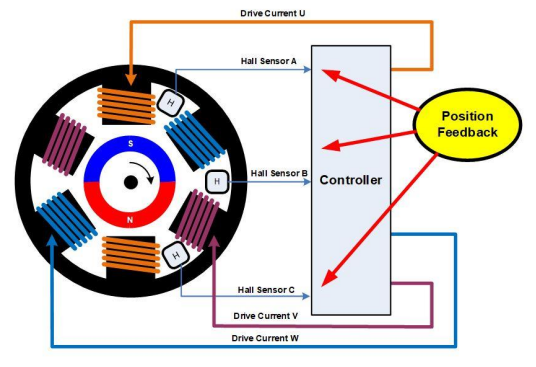
\includegraphics[width=0.5\textwidth]{assets/hallsensorsmetcontroller.png}
  \caption{BLDC met hall sensor en controller}
  \label{fig:hallsensorsmetcontroller.png}
 \end{figure}
\begin{figure}[H]
  \centering
  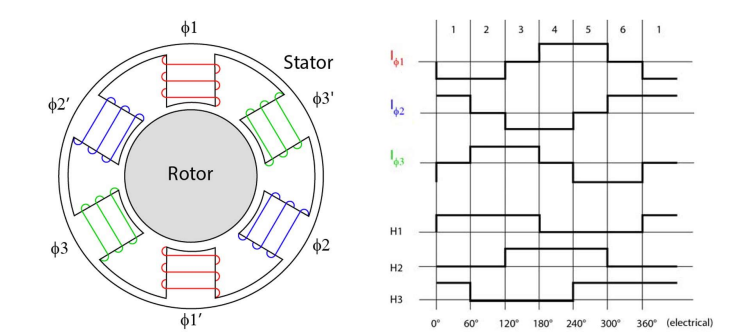
\includegraphics[width=0.6\textwidth]{assets/hallsensorgestuurdestromen.png}
  \caption{Stromen gestuurd door de hall sensor}
  \label{fig:hallsensorgestuurdestromen.png}
 \end{figure}
\begin{figure}[H]
  \centering
  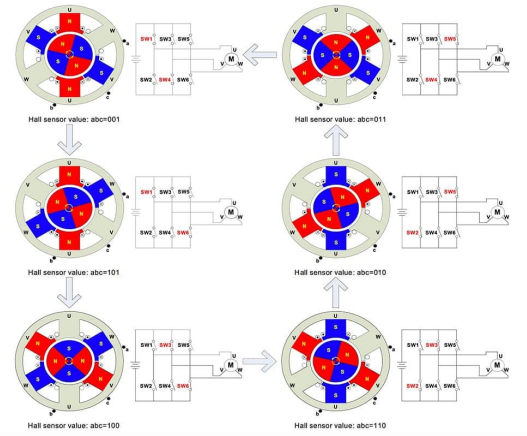
\includegraphics[width=0.6\textwidth]{assets/6stapscommutatie.png}
  \caption{6-staps commutatie}
  \label{fig:6stapscommutatie.png}
 \end{figure}
\subsection{Terug-emk (back-emf) van de BLDC motor}
Terwijl dat de rotor draait (met zijn magneten dus) zien de statorspoelen dus ook een veranderd magnetisch veld voorbij komen wat dus een spanning induceert in de spoel ($e = B \cdot l \cdot v$). Dit is het terug-emk en deze wordt groter naarmate de rotor sneller draait (zoals bij alle DC en AC machines). Wat er echter speciaal is, is dat deze een \textbf{trapezoïdale vorm} heeft i.p.v. een mooie sinus, zoals we kunnen zien in volgende figuur:
\begin{figure}[H]
  \centering
  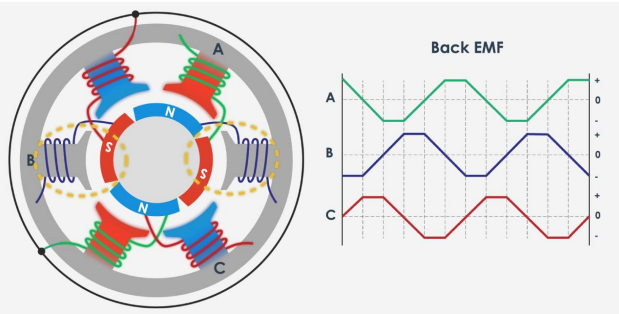
\includegraphics[width=0.6\textwidth]{assets/tegenemkbldc.png}
  \caption{Terug-emk van de BLDC motor}
  \label{fig:tegenemkbldc.png}
 \end{figure}
Dit komt doordat als een spoel volledig onder zo één magneetpool zit, ze eigelijk ongeveer een constant veld ziet steeds, dit maakt het constant in die emf-curve, pas wanneer de rotor verder draait en de zuidpool wegschuift terwijl de volgende noordpool binnekomt veranderd het veld snel van volledig negatief naar volledig positief wat dus die schuine flank geeft (uiteindelijk trapezium dus). Het feit dat dit wel een mooie sinus is bij de PMSM terwijl die ook permanente magenten gebruikt is door het feit dat daar de statorwikkelingen verdeeld zijn in plaats van geconcentreerd rond de polen zoals hier.
\begin{figure}[H]
  \centering
  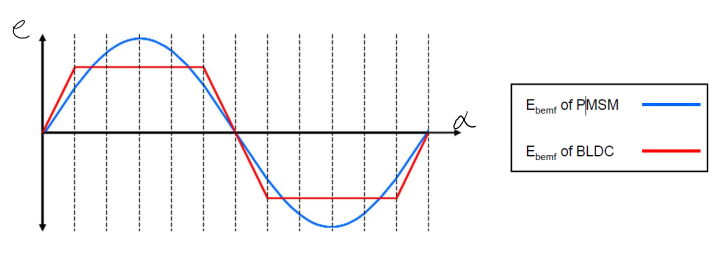
\includegraphics[width=0.7\textwidth]{assets/tegenemkbldcpmsm.png}
  \caption{Terug-emk van de BLDC en de PMSM motor}
  \label{fig:tegenemkbldcpmsm.png}
 \end{figure}
Nog iets belangrijk om te onthouden bij deze 2 motoren is dat doordat we permanente magneten gebruiken er geen vermogenverlies nodig is om het rotor veld zelf op te wekken.
\subsection{Koppel-toerental karakteristiek van de BLDC motor}
Net zoals de DC-machine heeft een BLDC motor een continue koppelzone (het groene) en ook een korstondige/intermittente zone (geel/snotgroen) erboven:
\begin{figure}[H]
  \centering
  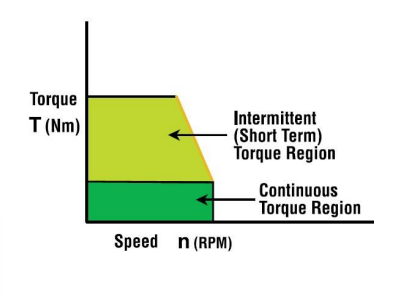
\includegraphics[width=0.5\textwidth]{assets/TNBLDC.png}
  \caption{Koppel-toerental karakteristiek van de BLDC motor}
  \label{fig:TNBLDC.png}
 \end{figure}
Er is ook een T-limiet (het plafond), dit is bepaald door de maximale stroom die door de wikkelingen continu kan gaan zonder oververhitting. In de gele zone kan je kort even werken met meer stroom/koppel. Ook is er een n-limiet, dit is eigelijk een begrenzing door mechanische factoren zoals de constructie van de rotor of lagers of door de schakel/commutatie elektronica zelf (de transistoren kunnen tot maar een bepaalde frequentie schakelen).
\newline
\newline
De volgende grafiek toont de verschillende lijnen voor verschillende spanningen, hoe hoger de spanning, hoe hoger de bereikbare snelheid bij een gegeven koppel. (Dit zagen we eerder bij de DC machine), het belangrijkste hier is omdat een BLDC via vermogenelektronica aangestuurd wordt, je niet gelimiteerd bent tot 1 van die lijnen, de controller kan elke spanning tot aan $V_1$ leveren. Dus eigelijk kan je in de praktijk eender welk werkingspunt in het oppervlak onder de $V_1$ lijn aannemen.
\begin{figure}[H]
  \centering
  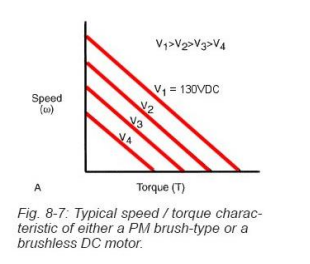
\includegraphics[width=0.5\textwidth]{assets/VlijnenBLDC.png}
  \caption{Spanningslijnen van de BLDC motor}
  \label{fig:VlijnenBLDC.png}
 \end{figure}
\subsection{BLDC vs (PM)Borstel DC motor}
Nu gaan we enkele voor- en nadelen vergelijken van de BLDC met de gewone (PM)DC motor.
\newline
\textbf{{\color{green}Voordelen} van de BLDC:}
\begin{itemize}
    \item Langere levensduur (geen borstels/commutator die slijten)
    \item Minder geluid en elektrische storing (geen vonken van de borstels)
    \item Makkelijker te koelen: Bij een BLDC zitten alle koperverliezen in de wikkelingen op de stator, die staat stil en is dus makkelijk te koelen, bij een PMDC zit het anker juist op de rotor, warmte afvoeren van een ronddraaiend deel is lastiger
    \item Beter rendement dankzij elektronische sturing
\end{itemize}
\textbf{{\color{red}Nadelen} van de BLDC:}
\begin{itemize}
 \item Hogere kost
 \item Trillingen bij lage snelheid (door de 6-staps commutatie)
 \item Complexe elektronica nodig (controller, hall sensoren, $\cdots$)
\end{itemize}
Een samenvattende figuur van voor en nadelen voor ook de inductiemotor en stappenmotor zien we in volgende figuur:
\begin{figure}[H]
  \centering
  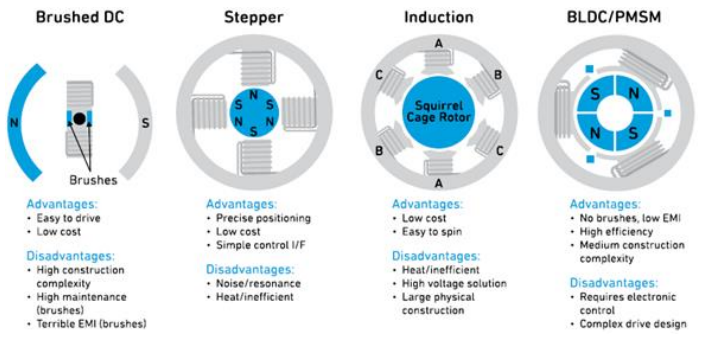
\includegraphics[width=0.8\textwidth]{assets/vergelijkingenmotore.png}
  \caption{Vergelijking van de verschillende motoren}
  \label{fig:vergelijkingenmotore.png}
 \end{figure}
\section{Reluctantie motoren}
Een reluctantie motor is een nieuw type motor, het positioneert zich als een concurrent van de inductiemachine. Het is een soort synchrone motor. Het bijzondere aan deze motor is dat \textit{de rotor enkel bestaat uit ijzer}, dus geen wikkelingen of magneten of kooi ofzo. Dit maakt het super goedkoop en robuust (geen koperverliezen op de rotor, geen dure magneten en praktisch INDESTRUCTABLE). Maar hoe werkt het?
\begin{figure}[H]
  \centering
  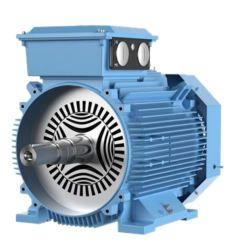
\includegraphics[width=0.4\textwidth]{assets/fotoreluctantiemotor.png}
  \caption{Reluctantie motor}
  \label{fig:fotoreluctantiemotor.png}
 \end{figure}
\subsection{Werking van de reluctantie motor}
We zagen dit concept al eerder maar deze motor werkt hier dus volledig op, namelijk het \textbf{reluctantiekoppel}. Reluctantie is de magnetische weerstand eigelijk, het is hoe makkelijk de flux door een pad kan vloeien en ijzer heeft een veel lagere reluctantie dan lucht. Het kernprincipe van deze motor is dat elk magnetisch systeem probeert zijn energie te minimaliseren, dus door zijn reluctantie te minimaliseren. Een stuk ijzer dat scheef staat tegenover een veld 'voelt' daardoor een koppel dat het terug wilt uitlijnen met dat veld (want het is het pad van minst reluctantie). Dit zien we in de volgende figuur:
\begin{figure}[H]
  \centering
  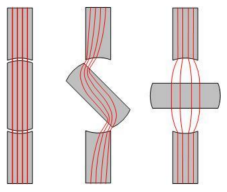
\includegraphics[width=0.4\textwidth]{assets/padvanminstreluctantie.png}
  \caption{Pad van minst reluctantie}
  \label{fig:padvanminstreluctantie.png}
 \end{figure}
In de volgende figuur zien we hoe dit toegepast wordt met de stator en de rotor, hoe meer overlap tussen de stator en rotortanden, hoe lager de reluctantie:
\begin{figure}[H]
  \centering
  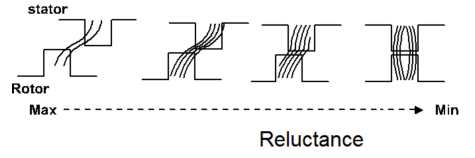
\includegraphics[width=0.8\textwidth]{assets/sgtatorrotorreluctantie.png}
  \caption{Overlap tussen stator en rotor}
  \label{fig:sgtatorrotorreluctantie.png}
 \end{figure}
Er zijn 2 varianten van reluctantiemotoren, we hebben de \textbf{synchrone reluctantie motor} en de \textbf{'switched' reluctantie motor} (SRM).
\begin{figure}[H]
  \centering
  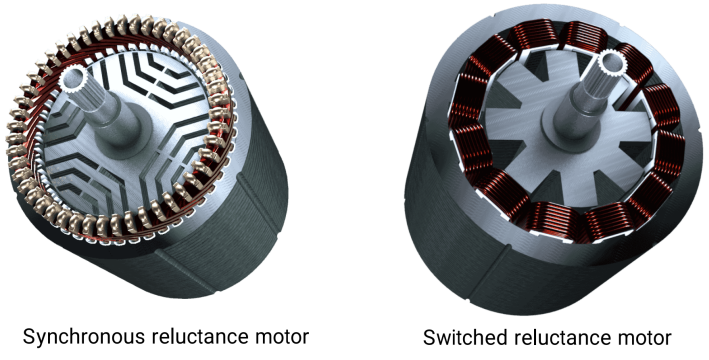
\includegraphics[width=0.6\textwidth]{assets/synchroneenswitchedreluctantiemotor.png}
  \caption{Varianten van reluctantiemotoren}
  \label{fig:synchroneenswitchedreluctantiemotor.png}
 \end{figure}
De \textbf{synchrone reluctantiemotor} heeft een rotor met interne 'flux barrieres' die voorkeursrichtingen voor de flux creëren, het wordt aangedreven door een gewoon draaiveld zoals bij de inductiemotor en loopt daarmee synchroon mee (geen slip)
\newline
\newline
De \textbf{'switched' reluctantiemotor} heeft een getande rotor en stator en wordt aangedreven door telkens een paar statorspoelen gericht aan en uit te schakelen (daarom 'switched'), dit is hoe steeds de dichtsbijzijnde rotortand telkens zo wilt uitlijnen met een bekrachtigde statortand zoals in die figuur die ik net toonde. Dit is een beetje gelijkaardig aan de BLDC, daar was het aantrekken met een magneet.
\subsection{Nadelen van de 'switched' reluctantiemotor}
De 'switched' reluctantiemotor heeft echter een paar nadelen, namelijk dat we een koppelrimpel hebben doordaat we steeds gaan uitlijnen met die tanden en dit zorgt voor \textbf{trillingen}. ook heeft het een \textbf{ingewikkelde constructie/sturing}, die dubbel getande geometrie is lastig te ontwerpen en verreist ook nauwkeurige sturing. ook is er veel \textbf{ijzerverzadiging} rond de uitgelijnde tanden wat het stroom-koppel verband minder lineair maakt en dus de sturing bemoeilijkt.
\subsection{Werking van de synchrone reluctantiemotor}
Het is dus de deze dat dan meer gebruikt wordt als we het gaan hebben over de reluctantie motor. De rotor is  hier opgebouwd uit gelamelleerd ijzer met halfronde luchtspleten (flux barrieres) die in lagen boven elkaar zitten, dit zie je in de figuur hieronder links. Dit maakt de opbouw eigelijk anisotroop, in de ene richting geleidt hij flux makkelijk (rood) en in de andere richting bijna niet (blauw). 
\begin{figure}[H]
  \centering
  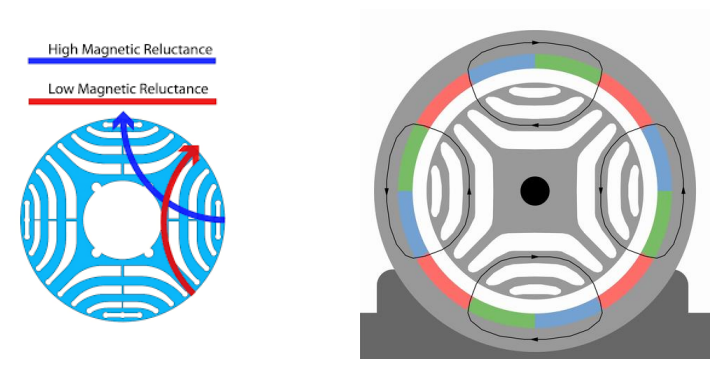
\includegraphics[width=0.6\textwidth]{assets/synchronereluctantiemotor.png}
  \caption{Synchrone reluctantiemotor}
  \label{fig:synchronereluctantiemotor.png}
 \end{figure}
Op het rechtse gedeelte van de figuur zien we blauwe/groene/rode zones, dit representeert de 3fases van de statorwikkelingen, er wordt een draaiveld opgewekt en net zoals bij de inductiemotor gaat de rotor voelen dat het niet perfect samen uitgelijnd is met het draaiveld en zich proberen uitlijnen dan. Omdat het veld blijft roteren blijft dit gebeuren en gaat de rotor dus mooi synchroon meedraaien met dat veld (geen slip). Ook omdat de rotor bij synchroon, continu draaien geen relatieve fluxverandering ondervindt zijn de ijzerverliezen in de rotor (tijdens continu bedrijf) minimaal, dit geeft deze motor een hoog rendement voor dit motortype toch. Geen rotorkoperverliezen hier en amper ijzerverliezen. Alleen bij transiënten (opstarten en belastinswissels) kunnen we wat verliezen hebben omdat de flux dan nog aan het 'instellen' is.
\section{Stappen motoren}
Dit moeten we niet uitgebreid meer kennen, dit is een volledig ander concept. We moeten vooral weten dat dit een positiegestuurde motor is en dat dit in plaats van een T-n karakteristiek een 'aantal stappen per omwenteling' heeft. Het werkt met 'open loop position control' (Elke puls die je stuurt doet de rotor exact één vaste, discrete hoek verspringen).
\newline
\newline
{\color{red}Alle slides/leerstof hier na moeten we niet meer kennen, dit is het einde van de leerstof}
\end{document}
